\documentclass[12pt,a4paper,final,twoside,onecolumn,titlepage]{book}

\newcommand*{\plogo}{\fbox{$\mathcal{PL}$}} % Generic publisher logo

%----------------------------------------------------------------------------------------
%	TITLE PAGE
%----------------------------------------------------------------------------------------

\newcommand*{\titleGP}{\begingroup % Create the command for including the title page in the document
\centering % Center all text
\vspace*{\baselineskip} % White space at the top of the page

\rule{\textwidth}{1.6pt}\vspace*{-\baselineskip}\vspace*{2pt} % Thick horizontal line
\rule{\textwidth}{0.4pt}\\[\baselineskip] % Thin horizontal line

{\LARGE Enterprise Integration \\ Opportunities and Challenges}\\[0.2\baselineskip] % Title

\rule{\textwidth}{0.4pt}\vspace*{-\baselineskip}\vspace{3.2pt} % Thin horizontal line
\rule{\textwidth}{1.6pt}\\[\baselineskip] % Thick horizontal line

\scshape % Small caps
University Information Systems Case Study \\[\baselineskip] % Tagline(s) or further description
Egypt,  2013\par % Location and year

\vspace*{2\baselineskip} % Whitespace between location/year and editors

Edited by \\[\baselineskip]
{\Large HAITHAM A. EL-GHAREEB \par} % Editor list
{\itshape The University of Mansoura \\ Egypt\par} % Editor affiliation

\vfill % Whitespace between editor names and publisher logo

%\plogo \\[0.3\baselineskip] % Publisher logo
{\large helghareeb@mans.edu.eg \\ http://www.helghareeb.me}\par % Publisher
{\scshape 2013} \\[0.3\baselineskip] % Year published

\endgroup}

\usepackage[export]{adjustbox}

\usepackage{makeidx}
\usepackage[utf8]{inputenc} %File encoding
\usepackage[T1]{fontenc} % Use EC fonts
\usepackage{ae} % Fonts for PDF files
\usepackage{textcomp} % Text-Companion-Symbols (e. g. \texteuro)
\usepackage[english]{babel} % Language selection
\usepackage{lmodern} % Latin Modern

\usepackage{pdfpages}

%New Section Added for Coding
\usepackage{amsmath}
\usepackage{algorithm2e}
\usepackage{amsfonts}
\usepackage{amssymb}
\usepackage{graphicx}
\usepackage{natbib}
\usepackage{listings}
\usepackage{color}
\usepackage{textcomp}
\usepackage{multirow}
\definecolor{listinggray}{gray}{0.9}
\definecolor{lbcolor}{rgb}{0.9,0.9,0.9}
\lstset{
	backgroundcolor=\color{white},
	tabsize=4,
	rulecolor=,
	language=csh,
        basicstyle=\scriptsize,
        upquote=true,
        aboveskip={1.5\baselineskip},
        columns=fixed,
        showstringspaces=false,
        extendedchars=true,
        breaklines=true,
        prebreak = \raisebox{0ex}[0ex][0ex]{\ensuremath{\hookleftarrow}},
        frame=single,
        showtabs=false,
        showspaces=false,
        showstringspaces=false,
        identifierstyle=\ttfamily,
        keywordstyle=\color[rgb]{0,0,1},
        commentstyle=\color[rgb]{0.133,0.545,0.133},
        stringstyle=\color[rgb]{0.627,0.126,0.941},
}

%End of New Section Added for Coding

\usepackage[english]{translator}
%Load the package
\usepackage[
nonumberlist, %do not show page numbers
acronym,      %generate acronym listing
toc,          %show listings as entries in table of contents
section]      %use section level for toc entries
{glossaries}

\usepackage{hyperref}

%Added on March 20, 2013 for fitting figures within Text Boundaries
\usepackage[export]{adjustbox}
\usepackage{tabularx}

%This Package is used for Margins
\usepackage[margin=3.0cm]{geometry}


%Generate a list of symboles
\newglossary[slg]{symbolslist}{syi}{syg}{List of symbols}

%Remove the dot at the end of glossary descriptions
\renewcommand*{\glspostdescription}{}

%Activate glossary commands
\makeglossaries

%These commands sort the lists
%makeindex -s filename.ist -t filename.alg -o filename.acr filename.acn
%makeindex -s filename.ist -t filename.glg -o filename.gls filename.glo
%makeindex -s filename.ist -t filename.slg -o filename.syi filename.syg

%Some entries for the list of symbols
\newglossaryentry{symb:Pi}{
name=$\pi$,
description={A mathematical constant whose value is the ratio of any circle's circumference to its diameter.},
sort=symbolpi, type=symbolslist
}


%Some acronyms
%\newacronym{AEHS}{AEHS}{Adaptive Educational Hypermedia Systems}

\newacronym{ANSI/IEEE}{ANSI/IEEE}{American National Standards Institute / Institute of Electrical and Electronics Engineers}
\newacronym{ARPA}{ARPA}{Advanced Research Projects Agency}
\newacronym{BPEL}{BPEL}{Business Process Execution Language}
\newacronym{BPEL4WS}{BPEL4WS}{Business Process Execution Language for Webservice}
\newacronym{BPMN}{BPMN}{Business Process Modeling Notation}
\newacronym{BPR}{BPR}{Business Process Reengineering}
\newacronym{CBA}{CBA}{Component Based Architecture}
\newacronym{DBMS}{DBMS}{Database Management System}
\newacronym{DCE}{DCE}{Distributed Computing Environment}
\newacronym{FIPA}{FIPA}{Foundation for Intelligent Physical Agents}
\newacronym{HTTP}{HTTP}{Hyper Text Transfer Protocol}
\newacronym{ISO/IEC}{ISO/IEC}{International Organization for Standardization / International Electrotechnical Commission}
\newacronym{ITS}{ITS}{Intelligent Tutoring System}
\newacronym{KAoS}{KAoS}{Knowledgeable Agent-oriented System}
\newacronym{KIF}{KIF}{Kowledge Interchange Format}
\newacronym{KQML}{KQML}{Knowledge Query and Manipulation Language}
\newacronym{MAS}{MAS}{Multi Agent System}
\newacronym{MIS}{MIS}{Management Information System}
\newacronym{MNAS}{MNAS}{Mobile News Agent System}
\newacronym{NAEP}{NAEP}{National Assessment of Education Process}
\newacronym{ROI}{ROI}{Return On Investment}
\newacronym{RPC}{RPC}{Remote Procedure Call}
\newacronym{SMTP}{SMTP}{Simple Mail Transfer Protocol}
\newacronym{SOI}{SOI}{Service Oriented Integration}
\newacronym{SW}{SW}{Software}
\newacronym{TQM}{TQM}{Total Quality Management}
\newacronym{UMIS}{UMIS}{University Management Information System}
\newacronym{VLE}{VLE}{Virtual Learning Environment}
\newacronym{W3C}{W3C}{World Wide Web Consortium}
\newacronym{WfMC}{WfMC}{Workflow Management Coalition}
\newacronym{WfMS}{WfMS}{Workflow Management System}
\newacronym{WOA}{WOA}{Web Oriented Architecture}
\newacronym{XPDL}{XPDL}{XML Process Definition Language}

\newacronym{AI}{AI}{Artificial Intelligence}
\newacronym{LIS}{LIS}{Library Information System}
\newacronym{MS}{MS}{Microsoft}
\newacronym{CMS}{CMS}{Course Management System}
\newacronym{ICT}{ICT}{Information and Communication Technology}
\newacronym{IMS}{IMS}{ (a.k.a ITIMS or IMS GLC): a global, nonprofit, member organization that strives to enable the growth and impact of learning technology in the education and corporate learning sectors worldwide.}
\newacronym{IMS QTI}{IMS QTI}{IMS - Question and Test Interoperability}
\newacronym{SIS}{SIS}{Student Information System}


%An acronym with a glossary entry
\newacronym{ADL}{ADL}{Advanced Distributed Learning\protect\glsadd{glos:ADL}}
\newacronym{AEHS}{AEHS}{Adaptive Educational Hypermedia Systems\protect\glsadd{glos:AEHS}}
\newacronym{AIEHS}{AIEHS}{Adaptive Intelligent Educational Hypermedia Systems\protect\glsadd{glos:AIEHS}}
\newacronym{ANN}{ANN}{Artificial Neural Network\protect\glsadd{glos:ANN}}
\newacronym{BA}{BA}{Business Analytics\protect\glsadd{glos:BA}}
\newacronym{BI}{BI}{Business Intelligence\protect\glsadd{glos:BI}}
\newacronym{BPM}{BPM}{Business Process Management\protect\glsadd{glos:BPM}}
\newacronym{BPMS}{BPMS}{Business Process Management System\protect\glsadd{glos:BPM}}
\newacronym{CASE}{CASE}{Computer assisted Systems Engineering\protect\glsadd{glos:CASE}}
\newacronym{CORBA}{CORBA}{Common Object Request Broker\protect\glsadd{glos:CORBA}}
\newacronym{CRM}{CRM}{Customer Relation Management\protect\glsadd{glos:CRM}}
\newacronym{DB}{DB}{Data Base\protect\glsadd{glos:DB}}
\newacronym{DM}{DM}{Data Mining\protect\glsadd{glos:DM}}
\newacronym{DW}{DW}{Data Warehouse\protect\glsadd{glos:DW}}
\newacronym{DSS}{DSS}{Decision Support System\protect\glsadd{glos:DSS}}
\newacronym{EA}{EA}{Enterprise Architecture\protect\glsadd{glos:EA}}
\newacronym{EAI}{EAI}{Enterprise Application Integration\protect\glsadd{glos:EAI}}
\newacronym{EIP}{EIP}{Enterprise Information Portal\protect\glsadd{glos:EIP}}
\newacronym{EIS}{EIS}{Enterprise Information System\protect\glsadd{glos:EIS}}
\newacronym{ELF}{ELF}{E-Learning Framework\protect\glsadd{glos:ELF}}
\newacronym{ERM}{ERM}{Enterprise Resource Management\protect\glsadd{glos:ERM}}
\newacronym{ERP}{ERP}{Enterprise Resource Planning\protect\glsadd{glos:ERP}}
\newacronym{ES}{ES}{Expert System\protect\glsadd{glos:ES}}
\newacronym{ESB}{ESB}{Enterprise Service Bus\protect\glsadd{glos:ESB}}
\newacronym{GSS}{GSS}{Group Support System\protect\glsadd{glos:GSS}}
\newacronym{IS}{IS}{Information System\protect\glsadd{glos:IS}}
\newacronym{IA}{IA}{Intelligent Agent\protect\glsadd{glos:IA}}
\newacronym{KMP}{KMP}{Knowledge Management Portal\protect\glsadd{glos:KMP}}
\newacronym{KMS}{KMS}{Knowledge Management System\protect\glsadd{glos:KMS}}
\newacronym{LMS}{LMS}{Learning Management System\protect\glsadd{glos:LMS}}
\newacronym{moodle}{moodle}{Modular Object Oriented Dynamic Learning Environment\protect\glsadd{glos:moodle}}
\newacronym{MSS}{MSS}{Management Support System\protect\glsadd{glos:MSS}}
\newacronym{OKI}{OKI}{Open Knowledge Initiative\protect\glsadd{glos:OKI}}
\newacronym{OLAP}{OLAP}{Online Analytical Processing\protect\glsadd{glos:OLAP}}
\newacronym{SCM}{SCM}{Supply Chain Management\protect\glsadd{glos:SCM}}
\newacronym{SOA}{SOA}{Service Oriented Architecture\protect\glsadd{glos:SOA}}
\newacronym{SOAP}{SOAP}{Simple Object Access Protocol\protect\glsadd{glos:SOAP}}
\newacronym{UDDI}{UDDI}{Universal Description Discovery and Integration\protect\glsadd{glos:UDDI}}
\newacronym{WSDL}{WSDL}{Webservice Description Language\protect\glsadd{glos:WSDL}}
\newacronym{XML}{XML}{Extensible Markup Language\protect\glsadd{glos:XML}}

%Some glossary terms
\newglossaryentry{glos:ADL}{name={ADL}, description = {ADL: Advanced Distributed Learning, established in 1997 to standardize and modernize training and education management and delivery. The Department of Defense (DoD) Office oversees the initiative. http://www.adlnet.gov}}

\newglossaryentry{glos:AEHS}{name={AEHS}, description = {Adaptive Hypermedia Systems as systems that refer to all hypertext and hypermedia systems which reflect some features of the user in the user model and apply this model to adapt various visible aspects of the system to the user. In other words, the system should satisfy three criteria: it should be a hypertext or hypermedia system; it should have a user model; it should be able to adapt the hypermedia using this model. Educational Hypermedia Systems are the most popular area for adaptive hypermedia research.}}

\newglossaryentry{glos:AIEHS}{name={AIEHS}, description = {Adaptive and Intelligent Educational Hypermedia System: Enhancing \gls{AEHS} with methods and techniques from \gls{ITS} creates the \gls{AIEHS}.}}

\newglossaryentry{glos:ANN}{name={ANN}, description = {Artificial Neural Network: a mathematical model inspired by biological neural networks. A neural network consists of an interconnected group of artificial neurons, and it processes information using a connectionist approach to computation. In most cases a neural network is an adaptive system that changes its structure during a learning phase. Neural networks are used to model complex relationships between inputs and outputs or to find patterns in data.}}

\newglossaryentry{glos:BA}{name={BA}, description = {Business Analytics: refers to the skills, technologies, applications and practices for continuous iterative exploration and investigation of past business performance to gain insight and drive business planning. \gls{BA} focuses on developing new insights and understanding of business performance based on data and statistical methods.}}

\newglossaryentry{glos:BI}{name={BI}, description = {Business Intelligence traditionally focuses on using a consistent set of metrics to both measure past performance and guide business planning of an enterprise, which is also based on data and statistical methods.}}

\newglossaryentry{glos:BPM}{name={BPM}, description = {Business Process Management is a systematic, structured approach to analyze, improve, control, and manage processes. Business Process is a series of inter-related activities that cross functional enterprise boundaries with individual inputs and outputs.}}

\newglossaryentry{glos:BPMS}{name={BPMS}, description = {Business Process Management System: is an \gls{EIS} that supports designing, administrating, and improving the Business Processes. Business Process is a series of inter-related activities that cross functional enterprise boundaries with individual inputs and outputs.}}

\newglossaryentry{glos:CASE}{name={CASE}, description = {Computer assisted Systems Engineering (CASE Tools): is the scientific application of a set of tools and methods to a software system which results in high-quality, defect-free, and maintainable software products. It also refers to methods for the development of \gls{IS} together with automated tools that can be used in the software development process.}}

\newglossaryentry{glos:CORBA}{name={CORBA}, description = {CORBA is a well-known specification for a middleware system that was developed in the 1990s by the Object Management Group. It was intended as an open standard that would allow the development of middleware to support distributed component communications and execution, plus provide a set of standard services that could be used by these components.}}

\newglossaryentry{glos:CRM}{name={CRM}, description = {Customer Relation Management: is a widely implemented model for managing a company's interactions with customers, clients, and sales prospects. It involves using technology to organize, automate, and synchronize business processes-principally sales activities, but also those for marketing, customer service, and technical support.}}

\newglossaryentry{glos:DB}{name={DB}, description = {Database is a collection of persistent data.}}

\newglossaryentry{glos:DM}{name={DM}, description = {Data Mining is the process that attempts to discover patterns in large data sets. It utilizes methods at the intersection of artificial intelligence, machine learning, statistics, and database systems.}}

\newglossaryentry{glos:DW}{name={DW}, description = {Data Warehouse: data warehouse or enterprise data warehouse (DW, DWH, or EDW) is a database used for reporting and data analysis. It is a central repository of data which is created by integrating data from multiple disparate sources. Data warehouses store current as well as historical data and are used for creating trending reports for senior management reporting such as annual and quarterly comparisons.}}

\newglossaryentry{glos:DSS}{name={DSS}, description = {Decision Support System: a computer-based information system that supports business or organizational decision-making activities. \gls{DSS}s serve the management, operations, and planning levels of an organization and help to make decisions, which may be rapidly changing and not easily specified in advance. \gls{DSS}s can be either fully computerized, human or a combination of both.}}

\newglossaryentry{glos:Enterprise}{name={Enterprise}, description = {Enterprise is simply a convenient generic term for any reasonably self-contained commercial, scientific, technical or other organization.}}

\newglossaryentry{glos:EA}{name={EA}, description = {Enterprise Architecture is the process of translating business vision and strategy into effective enterprise change by creating, communicating and improving the key requirements, principles and models that describe the enterprise's future state and enable its evolution. Practitioners of EA call themselves enterprise architects. An enterprise architect is a person responsible for performing this complex analysis of business structure and processes and is often called upon to draw conclusions from the information collected. By producing this understanding, architects are attempting to address the goals of \gls{EA}: Effectiveness, Efficiency, Agility, and Durability.}}

\newglossaryentry{glos:EAI}{name={EAI}, description = {Enterprise Application Integration integrates applications and systems using middleware. \gls{EAI} solutions are technology based but often not based on standards such as Web services. \gls{EAI} has two main integration patterns: hub and spoke and publish-subscribe. \gls{EAI} solutions using messaging middleware could be programmed differently to have such awareness.}}

\newglossaryentry{glos:EIS}{name={EIS}, description = {Enterprise Information System: is generally any kind of computing system that is of "enterprise class". This means typically offering high quality of service, dealing with large volumes of data and capable of supporting some large organization ("an enterprise"). \gls{EIS}s provide a technology platform that enables organizations to integrate and coordinate their business processes.}}

\newglossaryentry{glos:ELF}{name={ELF}, description = {E-Learning Framework, an international effort to develop a service-oriented approach to the development and integration of computer systems in the sphere of learning, research and education administration. Official Website: http://www.elframework.org }}

\newglossaryentry{glos:EIP}{name={EIP}, description = {Enterprise Information Portal: is a framework for integrating information, people and processes across organizational boundaries. It provides a secure unified access point, often in the form of a web-based user interface, and is designed to aggregate and personalize information through application-specific portlets. One hallmark of enterprise portals is the de-centralized content contribution and content management, which keeps the information always updated.}}

\newglossaryentry{glos:ERM}{name={ERM}, description = {Enterprise Resource Management: describes software that lets an enterprise manage user access to its network resources efficiently. \gls{ERM} software generally lets a user sign on to different enterprise systems and applications using the same password. \gls{ERM} software makes it easy for the enterprise to control and keep track of which systems and resources each user has access to, and provides consistent standards for creating and changing passwords.}}

\newglossaryentry{glos:ERP}{name={ERP}, description = {Enterprise Resource  Planning: systems integrates internal and external management information across an entire organization, embracing finance/accounting, manufacturing, sales and service, \gls{CRM}, etc. \gls{ERP} systems automate this activity with an integrated software application.}}

\newglossaryentry{glos:ES}{name={ES}, description = {Expert System: is a computer system that emulates the decision-making ability of a human expert. \gls{ES}s are designed to solve complex problems by reasoning about knowledge, like an expert, and not by following the procedure of a developer as is the case in conventional programming.}}

\newglossaryentry{glos:ESB}{name={ESB}, description = {Enterprise Service Bus: is an architectural pattern that has multiple motivations: Supports large numbers of service interactions in a manageable way, Provides support for advanced service interaction capability, such as transactions, store and forward, infrastructure services, security, quality of service, and so on, Supports a variety of interaction styles such as synchronous request/response, messaging, publish/subscribe, and events, Provides a robust, manageable, distributed integration infrastructure consistent with the principles of \gls{SOA}, Supports service routing and substitution, protocol transformations, and other message processing, Supports both Web Services and traditional \gls{EAI} communication standards and technologies.}}


\newglossaryentry{glos:GSS}{name={GSS}, description = {Group Support Systems: Facilitates decisions made by groups within the organization. Traditional meeting can last a long time and money. Collaborative computing systems, groupware, electronic meeting can run over the Web and provide video conferencing, audio conferencing in addition to meeting tools like electronic brainstorming, voting and document sharing.}}

\newglossaryentry{glos:IA}{name={IA}, description = {Intelligent Agent: is an autonomous entity which observes through sensors and acts upon an environment using actuators (i.e. it is an agent) and directs its activity towards achieving goals (i.e. it is rational). \gls{IA}s may also learn or use knowledge to achieve their goals. They may be very simple or very complex: a reflex machine such as a thermostat is an \gls{IA}, as is a human being, as is a community of human beings working together towards a goal.}}

\newglossaryentry{glos:IS}{name={IS}, description = {Information System can be defined technically as a set of interrelated components that collect (or retrieve), process, store, and distribute information to support decision making and control in an organization. In addition to supporting decision making, coordination, and control, information systems may also help managers and workers analyze problems, visualize complex subjects, and create new products}}

\newglossaryentry{glos:KMP}{name={KMP}, description = {Knowledge Management Portal: provides a platform to store information and knowledge into multiple place, exploit it and share it like never before. Helps organization to organically grow their knowledge base. In a typical organization, some 75\% of internal knowledge is trapped in one's email and desktop computers. Good information should be everywhere and nowhere near.}}

\newglossaryentry{glos:KMS}{name={KMS}, description = {Knowledge Management Systems: A \gls{KMS} is a computerized system designed to support the creation, storage, and dissemination of information. Such a system contains a central repository of information that is well structured and employs a variety of effective and easy to use search tools that users can use to find answers to questions quickly.}}

\newglossaryentry{glos:LMS}{name={LMS}, description = {Learning Management System is the software that automates the administration of training. \gls{LMS} registers users, tracks courses in a catalog, records data from learners, and provides reports to management. An \gls{LMS} is typically designed to handle courses by multiple publishers and providers. It usually doesn't include its own authoring capabilities. Instead, it focuses on managing courses created by a variety of other sources.}}

\newglossaryentry{glos:moodle}{name={moodle}, description = {Moodle: an Open Source \gls{LMS}. Stands for: Modular Object Oriented Dynamic Learning Environment. Official Moodle website: http://moodle.org/}}

\newglossaryentry{glos:MSS}{name={MSS}, description = {Management Support System is the support of management tasks by the application of technologies. Sometimes called \gls{DSS}s or \gls{BI}.}}

\newglossaryentry{glos:OKI}{name={OKI}, description = {OKI: Open Knowledge Initiative, an organization responsible for the specification of software interfaces comprising a \gls{SOA} based on high level service definitions. Official Website: www.okiproject.org}} 

\newglossaryentry{glos:OLAP}{name={OLAP}, description = {Online Analytical Processing: is an approach to answering multidimensional analytical (MDA) queries swiftly. \gls{OLAP} is part of the broader category of \gls{BI}, which also encompasses relational database report writing and \gls{DM}. Typical applications of \gls{OLAP} include business reporting for sales, marketing, management reporting, \gls{BPM} (\gls{BPM}), budgeting and forecasting, financial reporting and similar areas, with new applications coming up, such as agriculture.}}

\newglossaryentry{glos:SCM}{name={SCM}, description = {Supply Chain Management:is the management of a network of interconnected businesses involved in the provision of product and service packages required by the end customers in a supply chain. \gls{SCM} spans all movement and storage of raw materials, work-in-process inventory, and finished goods from point of origin to point of consumption.}}

\newglossaryentry{glos:SOA}{name={SOA}, description = {Service Oriented Architecture: There is no agreed upon definition for \gls{SOA}. Refer to section \ref{SOADefinition} presented at page \pageref{SOADefinition} for more information.}}

\newglossaryentry{glos:SOAP}{name={SOAP}, description = {SOAP, originally defined as Simple Object Access Protocol, is a protocol specification for exchanging structured information in the implementation of Web Services in computer networks. It relies on Extensible Markup Language (\gls{XML}) for its message format, and usually relies on other Application Layer protocols, most notably \gls{HTTP} and \gls{SMTP}, for message negotiation and transmission.}}

\newglossaryentry{glos:UDDI}{name={UDDI}, description = {Universal Description, Discovery and Integration (\gls{UDDI}) is a platform independent, Extensible Markup Language (\gls{XML})-based registry by which businesses worldwide can list themselves on the Internet, and a mechanism to register and locate web service applications. \gls{UDDI} is an open industry initiative, sponsored by the Organization for the Advancement of Structured Information Standards (OASIS), for enabling businesses to publish service listings and discover each other, and to define how the services or software applications interact over the Internet.}}

\newglossaryentry{glos:WSDL}{name={WSDL}, description = {The Web Services Description Language is an \gls{XML}-based interface description language that is used for describing the functionality offered by a web service. A \gls{WSDL} description of a web service (also referred to as a \gls{WSDL} file) provides a machine-readable description of how the service can be called, what parameters it expects, and what data structures it returns. It thus serves a roughly similar purpose as a method signature in a programming language.}}

\newglossaryentry{glos:XML}{name={XML}, description = {Extensible Markup Language is a markup language that defines a set of rules for encoding documents in a format that is both human-readable and machine-readable. It is defined in the \gls{XML} 1.0 Specification produced by the \gls{W3C}, and several other related specifications, all gratis open standards. The design goals of \gls{XML} emphasize simplicity, generality, and usability over the Internet. It is a textual data format with strong support via Unicode for the languages of the world. Although the design of \gls{XML} focuses on documents, it is widely used for the representation of arbitrary data structures, for example in web services.}}

\usepackage[utf8]{inputenc}
\usepackage{amsmath}
\usepackage{amsfonts}
\usepackage{amssymb}
\usepackage{graphicx}
\usepackage{natbib}

\author{Haitham A. El-Ghareeb, Ph.D. \\ \texttt{helghareeb@mans.edu.eg}}
\title{Associate Professor}
\date{\today}

\makeindex


\begin{document}
\frontmatter

%\maketitle
%\pagestyle{empty} % Removes page numbers

\thispagestyle{empty}
\titleGP % This command includes the title page


\cleardoublepage
\thispagestyle{empty}
\begin{center}
-= To my Family =- \\
\textit{Haitham A. El-Ghareeb, Ph.D.}
\end{center}

\begin{flushright}
March, 2013
\end{flushright}

\cleardoublepage
\phantomsection
\chapter{Acknowledgment}
%\addcontentsline{toc}{chapter}{Acknowledgment}
\thispagestyle{empty}
\paragraph*{
First and foremost, I thank ALLAH for giving me incentive to go on and finish this work, and every other work have been finished and giving me glimpses of heavenly hope in the darkest times.}
\paragraph*{I would like to thank Professor Alaa El-Din Mohamed Riad, Dean of Faculty of Computers and Information Sciences at Mansoura University; at the time of writing these lines, for his unlimited support and encouragement, for providing me with valuable insights and encouraging me to always do better, for always giving me great and valuable ideas to enhance my work.}
\paragraph*{I would like to thank Dr.Hamy El-Minir, head of communications department of Misr High Institute of Engineering for his support and motivation.}

\paragraph*{I would like to thank Dr.Hazem M. El-Bakry for the insightful discussions, and ideas, for taking long times to discuss smallest details.}

\paragraph*{I would like to thank Dr.Ahmed El-Said Hassan for the insightful discussions, ideas, and for taking long times for discussions.}

\paragraph*{I would like to thank Asma Samir for her contribution in building Sanay3y Application, and her great work in documenting the project.}

\paragraph*{My Family, you are the people whom without I could not have continued the journey to the day I witness this book alive. Thanks for always being there to support me, every single moment, with everything you can, when I was about to lose hope and trust in me being able to continue through the darkness, trying to reach the goal through long nights of mess, you were there, through long distances you were pushing me forward by your support, encouragement, guidance, and help. Thanks to ALLAH, I am really blessed with amazing family like you. I Love You all!}

\thispagestyle{empty}

\begin{flushright}
\textit{Haitham A. El-Ghareeb} \\
March, 2013
\end{flushright}

\cleardoublepage
\phantomsection
\listoffigures
\listoftables
\tableofcontents

\chapter{Preface}
%\addcontentsline{toc}{chapter}{Preface}
Today, organizations use computer-based \gls{IS} to better manage operations in the digital world. These organizations use information systems to provide high-quality goods and services as well as to gain or sustain competitive advantage over rivals. In addition to helping organizations to be competitive, information systems have contributed to tremendous societal changes. Chapter \ref{EISandEA} presented at page \pageref{EISandEA} presents different roles of \gls{IS} as we move into the digital world and how they have helped fuel decision making. We then highlight what information systems are, how \gls{DSS} have evolved to become a vital part of modern organizations, what are the main technologies behind \gls{DSS}, and why this understanding is necessary to become an effective manager in the digital world. Chapter concludes by discussing \gls{EA}, its components, and different examples of \textit{defacto} standards.\index{Enterprise Architecture}

Technical agility refers to the ability to quickly change the type and flow of information within an enterprise. Technical agility parameters are affected by \gls{EA}. IT advance has not yet satisfied business requirements due to improper software architectures. \gls{SOA} addresses technical agility requirements by presenting composability, modularity, and loose coupling concepts as services that wrap underlying IT infrastructure, databases, and legacy systems and present them via standard interface. There is a need to stabilize IT infrastructure rather than developing new ones and \gls{SOA} enables this stabilization. Enterprises should balance IT to become better positioned and more agile. Services are the building Blocks of an agile enterprise.\index{Enterprise Architecture} \index{Service Oriented Architecture}

Chapter \ref{SWArchitectureandIntegration} presented at page \pageref{SWArchitectureandIntegration} discusses the importance of \gls{EA} in meeting systems non-functional requirements and examines different software architecture paradigms, driving and restraining forces for each one in meeting systems integration as one of the most desirable requirement. Integration has different techniques, and different software architecture paradigms can address different techniques. This chapter presents a proposed mapping of different software architecture paradigms to different integration techniques while highlighting driving forces that encourages software architects to utilize it and restraining forces that discourages architects from utilizing them.\index{Enterprise Architecture}

\gls{SOA} as a design pattern that presents systems as collection of reusable services that can be exposed and consumed on the Internet with standard interfaces has many advantages that can be achieved on technical, managerial, and implementation aspects of the system. Chapter \ref{SOA} presented at page \pageref{SOA} discusses advantages of \gls{SOA}, different \gls{SOA} technologies, focusing on Webservices as main \gls{SOA} enablers. Chapter discusses \gls{ESB} and highlighting Microsoft BizTalk Server as one of the major \gls{ESB} implementations. Chapter concludes with answers of important \gls{SOA} questions.\index{Service Oriented Architecture}

Business agility is a new paradigm that is a solution for maintaining enterprise competitive advantage. Business improvement approaches, such as Total Quality Management, Business Process Reengineering, and Workflow Management Systems attempted to satisfy business agility concepts and requirements, but suffered from fatal limitations like lack of concepts definition and measurement, lack of practical implementation, and failure to support ongoing change. The three business improvement approaches realized the need for \gls{BPM} that is the key to business agility. \gls{BPMS} are \gls{IS}s that enable implementation of \gls{BPM}. Current IT infrastructure and \gls{IS}s architecture do not satisfy \gls{BPMS} objectives. \gls{SOA} as a design pattern addresses technical agility that satisfies \gls{BPMS} objectives in order to achieve business agility. \index{Service Oriented Architecture}

Chapter \ref{BPMandSOA} presented at page \pageref{BPMandSOA} presents a coupling model of \gls{BPMS} and \gls{SOA} in order to satisfy process and technical agility aspects of business agility. Proposed model utilizes standards available for mapping \gls{BPM} concepts via \gls{BPMS} into \gls{SOA}, and consists of three layers: Business, Business Services, and Application Services. Business layer enables business executives to handle business processes as information, \gls{BPMS} resides in this layer. Business services layer is the layer that maps \gls{BPM} concepts and requirements addressed by \gls{BPMS} into \gls{SOA} based IT infrastructure and \gls{EIS}s. Application Services layer holds the core services ready to be consumed by different \gls{BPMS} and shared among enterprises.
\index{Enterprise Information System}\index{Service Oriented Architecture}

Integrating \gls{UMIS} and \gls{LMS}  can be achieved effectively, efficiently, and with minor modifications of both systems via \gls{SOA} utilization. \gls{SOA} can also be useful in integrating long decades and efforts of adaptive and intelligent features of e-Learning in today's \gls{IS}s. Both \gls{UMIS} and \gls{LMS}; as the two major components of learning \gls{IS}s can make use of adaptive and intelligent features became available over decades. Adaptive and intelligent features in \gls{IS}s are many, and they can be utilized in new learning systems. Presenting adaptive and intelligent features as services with standard interfaces will allow different e-Learning systems to adopt them, so they will be reusable and newly introduced \gls{IS}s will not have to redo the work again, besides, wrapping adaptive and intelligent features with standard interfaces will present a separation of interests that help adaptive and intelligent features researchers and developers to focus more on their target and transfer the responsibility of utilizing those features in different \gls{IS}s to \gls{IS}s specialists. Today's e-Learning \gls{IS} architects can make use of \gls{SOA} in integrating major e-Learning components together, side by side with adaptive and intelligent features to provide students with personalized learning environment. \index{Service Oriented Architecture}

Chapter \ref{LMSFromMonolothicToServices} presented at page \pageref{LMSFromMonolothicToServices} reviews e-Learning different models and the challenges facing e-Learning nowadays, supposing solution to those challenges. Reviewing the e-Learning proposed systems, architectures, and frameworks starting from traditional e-Learning systems through adaptive e-Learning systems supported by intelligent e-Learning features, methods, and techniques yields e-Learning researchers to Services based Adaptive and Intelligent e-Learning Systems.

One of the critical limitations of a newly established educational institution is the lack of available well prepared courses. It is more applicable to use widely available courses that might be higher in quality than preparing new courses. Current \gls{CMS}s do not exploit courses shareability. Chapter \ref{CMS} presented at page \pageref{CMS} addresses this shortage by presenting a \gls{CMS} to highlight automated discovering and importing of courses maintained and managed by external \gls{CMS}s. Proposed \gls{CMS} architecture utilizes \gls{SOA} design pattern to integrate different \gls{CMS}s on service level. Proposed \gls{CMS} consists of two layers: Presentation layer and Service Layer. Presentation layer is responsible for interacting with user either via displaying information or receiving user inputs. Service layer contains core system services. Service layer is divided into three sub layers: orchestration layer, application services layer, and agents layer. Orchestration layer holds business logic required by system processes. Application services layer contains set of stateless services that are capable of performing certain tasks. Agents layer presents the suggested required software agents to serve the overall system. Suggested agents are: Discoverer, Ranker, Tracker, and Analyzer software agents. Integration between software agents and Web services is achieved by utilizing \gls{SOA}. Proposed \gls{CMS} facilitates integration between different \gls{CMS} in order to share resources of educational institutions.\index{Service Oriented Architecture}

Mobile Learning (M-Learning) is an approach to e-Learning that utilizes mobile devices. \gls{LMS} should enable M-Learning. Unfortunately, M-Learning is not the same at each educational institution. Assessment is one of the learning activities that can be achieved electronically and via mobile device. Mobile assessment relies on services that are not part of the \gls{LMS}. Integrating different external systems and services to be virtually part of \gls{LMS} is one of integration challenges. Chapter \ref{MobileDevicesInLMS} presented at page \pageref{MobileDevicesInLMS} presents a \gls{SOA} to integrate mobile assessment in \gls{LMS}. Proposed Architecture consists of two layers: Interface layer, and Service layer. Interface layer interacts with instructors and learners via portals, and with external organization services via Web services. Service layer contains core system services and has three sub layers: Orchestration, Application Services, and Agents layer. Orchestration layer is the layer that holds business logic required by system processes. Application Services layer contains set of stateless services that are capable of performing certain tasks. Agents layer presents the suggested required software agents to serve the overall system. Suggested agents are Analyzer and Tracker. Analyzer is required to analyze students assessments to detect learning deficiencies. Tracker agent tracks students to remind with missing assessments. \gls{SOA} facilitated integration of software agents within \gls{LMS}, and implementation of new processes to support learning.\index{Service Oriented Architecture}

Several types of Information and Communication Technology "ICT" have been utilized in the learning process to overcome time and place challenges. Learning delivery models are: traditional, distance, and hybrid learning. Hybrid learning attempts to maintain the best of traditional learning and provides the hopes and objectives of distance learning in a model that maintains the learning process on the right road. The widespread of Web 2.0; the Internet created by collaborative activities of different users resulted in the appearance of the acronym (e-Learning 2.0). Web 2.0 is a big resource that changed the way everyone around thinks about and accesses the Internet, and greatly will touch the coming generations; the generations that we are currently presenting education to. e-Learning 2.0 is supposed to make use of different Web 2.0 capabilities. From our perspective, e-Learning 2.0 shall be introduced into the lecture itself. This chapter presents taxonomy of Web 2.0 technologies, highlighting how, and when they can be used within learning institutions in enhancing the learning process. Web 2.0 technologies can be classified into In-Lecture and After-Lecture technologies based on their capabilities to support required activities for each class. Chapter \ref{Web2.0InLMS} presented at page \pageref{Web2.0InLMS} highlights different studies that show the importance and need from both instructors and students to utilize Web 2.0 technologies in learning institutions, presents different ways to use Web 2.0 technologies, and concludes with future research directions about Web 2.0 adoption in learning institutions. \gls{SOA} is a design pattern that presents infrastructure architecture, information architecture, and software architecture as composable services that wrap legacy systems and can be utilized in new systems. This chapter highlights the importance of \gls{SOA} in adopting Web 2.0 technologies in current lecture model.\index{Service Oriented Architecture}

To help universities achieve their goals, it is important to align managerial functionality side by side with educational aspects. Universities consume University Management Information Systems (\gls{UMIS}) to handle managerial aspects as they do with \gls{LMS}s (\gls{LMS}) to achieve learning objectives. \gls{UMIS} advances \gls{LMS} by decades and has reached stable and mature consistency level. \gls{LMS} is the newly acquired solution in Universities; compared to \gls{UMIS}, and so adopting \gls{LMS}s in universities can be achieved via three different deployment approaches. First approach believes in \gls{LMS} ability to replace \gls{UMIS} and performing its functionality. 
Second approach presents the idea of extending \gls{UMIS} to include \gls{LMS} functionality. Third approach arises from the shortages of the two proposed approaches and present integration between both as the appropriate deployment approach. \gls{SOA} is a design pattern that can be used as a suitable architectural solution to align \gls{UMIS} and \gls{LMS}. \gls{SOA} can be utilized in universities to overcome some of \gls{IS} challenges like the integration between \gls{UMIS} and \gls{LMS}. \index{Service Oriented Architecture}
Chapter \ref{EvaluationOfSOA} presented at page \pageref{EvaluationOfSOA} presents the current situation at Mansoura University; Egypt, presents integration as the most suitable solution, and evaluates three different implementation techniques: Dynamic Query, Stored Procedure, and Web services. Evaluation concludes that though \gls{SOA} enhanced many different aspects of both \gls{UMIS} and \gls{LMS}; and consequently university overall. It is not recommended to adopt \gls{SOA} via Web services as the building unit of the system, but as the interdisciplinary interface between systems.\index{Service Oriented Architecture}

Mobile information agents are mobile agents that retrieve information to end users. Chapter \ref{MobileInformationAgents} presented at page \pageref{MobileInformationAgents} presents a new architecture for \gls{MNAS} (\gls{MNAS}) that is based on a mobile information agents to retrieve news to users from different news servers. Several approaches for implementing \gls{MNAS} are illustrated and comparative analysis is performed to identify the most suitable one. \gls{MNAS} components are: Mobile News Agent that retrieves news to user, Directory Server that is the central manager server, and News Servers that hold different news categories and contents. \gls{MNAS} provides the client an easy to use interface to specify preferred news categories, a client application that initiates the mobile news agent which heads directly to the directory server to retrieves list of news servers that contain news matches user preferences, and searches all news servers and collects news to finally return to client. \gls{MNAS} proves that mobile information agent technology can not just be used in all information retrieval systems, because under some conditions, it might loose some of its advantages. \gls{MNAS} tries to find out the most appropriate information retrieval systems conditions to implement mobile information agent technology.\index{Service Oriented Architecture}.

\mainmatter

\chapter{EIS and EA}
\label{EISandEA}
\index{Enterprise Information System}
\section{Introduction}
Today, organizations use computer-based \gls{IS} to better manage operations in the digital world. These organizations use information systems to provide high-quality goods and services as well as to gain or sustain competitive advantage over rivals. In addition to helping organizations to be competitive, information systems have contributed to tremendous societal changes. An \gls{IS} can be defined technically as a set of interrelated components that collect (or retrieve), process, store, and distribute information to support decision making and control in an organization. In addition to supporting decision making, coordination, and control, information systems may also help managers and workers analyze problems, visualize complex subjects, and create new products \cite{MIS-DigitalFirm}. \gls{IS} contain information about significant people, places, and things within the organization or in the environment surrounding it. By information we mean data that have been shaped into a form that is meaningful and useful to human beings. Data, in contrast, are streams of raw facts representing events occurring in organizations or the physical environment before they have been organized and arranged into a form that people can understand and use. 

This chapter presents different roles of \gls{IS} as we move into the digital world and how they have helped fuel decision making. We then highlight what information systems are, how \gls{DSS} have evolved to become a vital part of modern organizations, what are the main technologies behind \gls{DSS}, and why this understanding is necessary to become an effective manager in the digital world. Chapter concludes by discussing \gls{EA}, its components, and different examples of \textit{defacto} standards.\index{Enterprise Architecture}

\section{Management Support System}
\gls{MSS} is the support of management tasks by the application of technologies. Sometimes called \gls{DSS}s or \gls{BI} \cite{MNAS02}. \gls{MSS} include:
\index{Management Support System}
\begin{itemize}
\item \gls{DSS} \cite{Wiki-DSS}: is a computer-based \gls{IS} that supports business or organizational decision-making activities. \gls{DSS}s serve the management, operations, and planning levels of an organization and help to make decisions, which may be rapidly changing and not easily specified in advance. \gls{DSS}s can be either fully computerized, human or a combination of both.
\item \gls{BA} \cite{Wiki-BA}: refers to the skills, technologies, applications and practices for continuous iterative exploration and investigation of past business performance to gain insight and drive business planning. \gls{BA} focuses on developing new insights and understanding of business performance based on data and statistical methods. In contrast, \gls{BI} traditionally focuses on using a consistent set of metrics to both measure past performance and guide business planning, which is also based on data and statistical methods.
\gls{BA} makes extensive use of data, statistical and quantitative analysis, explanatory and predictive modeling, and fact-based management to drive decision making. Analytic may be used as input for human decisions or may drive fully automated decisions. \gls{BI} is querying, reporting, \gls{OLAP}, and "alerts".
\item \gls{DM}\cite{Wiki-DM}: is the process that attempts to discover patterns in large data sets. It utilizes methods at the intersection of artificial intelligence, machine learning, statistics, and \gls{DB} systems. The overall goal of the \gls{DM} process is to extract information from a data set and transform it into an understandable structure for further use. Aside from the raw analysis step, it involves \gls{DB} and data management aspects, data preprocessing, model and inference considerations, interesting metrics, complexity considerations, post-processing of discovered structures, visualization, and online updating.
\item \gls{DW} \cite{Wiki-DW}: is a \gls{DB} used for reporting and data analysis. It is a central repository of data which is created by integrating data from multiple disparate sources. Data warehouses store current as well as historical data and are used for creating trending reports for senior management reporting such as annual and quarterly comparisons.
The data stored in the warehouse are uploaded from the operational systems (such as marketing, sales etc.). The data may pass through an operational data store for additional operations before they are used in the DW for reporting.
\item \gls{BI} \cite{Wiki-BI}: is the ability of an organization to collect, maintain, and organize data. This produces large amounts of information that can help develop new opportunities. Identifying these opportunities, and implementing an effective strategy, can provide a competitive market advantage and long-term stability. BI technologies provide historical, current and predictive views of business operations. Common functions of \gls{BI} technologies are reporting, online analytical processing, analytic, \gls{DM}, process mining, complex event processing, business performance management, benchmarking, text mining, predictive analytic and prescriptive analytic.
The goal of modern \gls{BI} deployments is to support better business decision-making.
\item \gls{OLAP} \cite{Wiki-OLAP}: is an approach to answering multi-dimensional analytical (MDA) queries swiftly. \gls{OLAP} is part of the broader category of \gls{BI}, which also encompasses relational \gls{DB} report writing and \gls{DM}. Typical applications of \gls{OLAP} include business reporting for sales, marketing, management reporting, \gls{BPM}, budgeting and forecasting, financial reporting and similar areas, with new applications coming up, such as agriculture. The term \gls{OLAP} was created as a slight modification of the traditional \gls{DB} term OLTP (Online Transaction Processing). \gls{OLAP} tools enable users to analyze multidimensional data interactively from multiple perspectives. \gls{OLAP} consists of three basic analytical operations: consolidation (roll-up), drill-down, and slicing and dicing. Consolidation involves the aggregation of data that can be accumulated and computed in one or more dimensions. For example, all sales offices are rolled up to the sales department or sales division to anticipate sales trends. By contrast, the drill-down is a technique that allows users to navigate through the details. For instance, users can view the sales by individual products that make up a regions sales. Slicing and dicing is a feature whereby users can take out (slicing) a specific set of data of the \gls{OLAP} cube and view (dicing) the slices from different viewpoints.
\item \gls{CASE} \cite{Wiki-CASE}: is the scientific application of a set of tools and methods to a software system which results in high-quality, defect-free, and maintainable software products. It also refers to methods for the development of \gls{IS} together with automated tools that can be used in the software development process.
\item \gls{GSS} \cite{MNAS02} Facilitates decisions made by groups within the organization. Traditional meeting can last a long time and money. Collaborative computing systems, groupware, electronic meeting can run over the Web and provide video conferencing, audio conferencing in addition to meeting tools like electronic brainstorming, voting and document sharing. \index{Group Support Systems}
\item \gls{EIS}\cite{Wiki-EIS}: is generally any kind of computing system that is of "\gls{glos:Enterprise} class". This means typically offering high quality of service, dealing with large volumes of data and capable of supporting some large organization ("an enterprise"). \gls{EIS}s provide a technology platform that enables organizations to integrate and coordinate their business processes. An \gls{EIS} provides a single system that is central to the organization and that ensures information can be shared across all functional levels and management hierarchies. Enterprise systems create a standard data structure and are invaluable in eliminating the problem of information fragmentation caused by multiple information systems within an organization. A typical \gls{EIS} would be housed in one or more data centers, would run enterprise software, and could include applications that typically cross organizational borders such as content management systems. The word enterprise can have various connotations. Frequently the term is used only to refer to very large organizations. However, the term may be used to mean virtually anything, by virtue of it having become the latest corporate-speak buzzword.
\index{Enterprise Information System}
\item \gls{EIP} \cite{Wiki-EIP}: is a framework for integrating information, people and processes across organizational boundaries. It provides a secure unified access point, often in the form of a web-based user interface, and is designed to aggregate and personalize information through application-specific portlets. One hallmark of enterprise portals is the de-centralized content contribution and content management, which keeps the information always updated.
\item \gls{ERM} \cite{Wiki-ERM}: describes software that lets an enterprise manage user access to its network resources efficiently. \gls{ERM} software generally lets a user sign on to different enterprise systems and applications using the same password. \gls{ERM} software makes it easy for the enterprise to control and keep track of which systems and resources each user has access to, and provides consistent standards for creating and changing passwords. One system administrator can usually manage user access to all platforms and to the applications on these platforms that require controlled access.
\item \gls{ERP} \cite{Wiki-ERP}: systems integrate internal and external management information across an entire organization, embracing finance/accounting, manufacturing, sales and service, \gls{CRM}, etc. \gls{ERP} systems automate this activity with an integrated software application. The purpose of \gls{ERP} is to facilitate the flow of information between all business functions inside the boundaries of the organization and manage the connections to outside stakeholders. \gls{ERP} systems can run on a variety of computer hardware and network configurations, typically employing a \gls{DB} as a repository for information.
\item \gls{CRM} \cite{Wiki-CRM}:  is a widely implemented model for managing a company's interactions with customers, clients, and sales prospects. It involves using technology to organize, automate, and synchronize business processes; principally sales activities, but also those for marketing, customer service, and technical support. The overall goals are to find, attract, and win new clients, service and retain those the company already has, entice former clients to return, and reduce the costs of marketing and client service. \gls{CRM} describes a company-wide business strategy including customer-interface departments as well as other departments. Measuring and valuing customer relationships is critical to implementing this strategy.
\item \gls{SCM} \cite{Wiki-SCM}: is the management of a network of interconnected businesses involved in the provision of product and service packages required by the end customers in a supply chain. \gls{SCM} spans all movement and storage of raw materials, work-in-process inventory, and finished goods from point of origin to point of consumption.
Another definition is provided by the APICS Dictionary when it defines \gls{SCM} as the "design, planning, execution, control, and monitoring of supply chain activities with the objective of creating net value, building a competitive infrastructure, leveraging worldwide logistics, synchronizing supply with demand and measuring performance globally."
\item \gls{KMS} \cite{Wiki-KMS}: A \gls{KMS} is a computerized system designed to support the creation, storage, and dissemination of information. Such a system contains a central repository of information that is well structured and employs a variety of effective and easy to use search tools that users can use to find answers to questions quickly. \index{Knowledge Management System}
\item \gls{KMP} \cite{Wiki-KMP}: provides a platform to store information and knowledge into multiple place, exploit it and share it like never before. Helps organization to organically grow their knowledge base. In a typical organization, some 75\% of internal knowledge is trapped in one's email and desktop computers. Good information should be everywhere and nowhere near.
\item \gls{ES} \cite{Wiki-ES}: is a computer system that emulates the decision-making ability of a human expert. \gls{ES}s are designed to solve complex problems by reasoning about knowledge, like an expert, and not by following the procedure of a developer as is the case in conventional programming.The first \gls{ES}s were created in the 1970s and then proliferated in the 1980s. \gls{ES}s were among the first truly successful forms of AI software. \index{Expert System}
An \gls{ES} has a unique structure, different from traditional programs. It is divided into two parts, one fixed, independent of the \gls{ES}: the inference engine, and one variable: the knowledge base. To run an \gls{ES}, the engine reasons about the knowledge base like a human. In the 80s a third part appeared: a dialog interface to communicate with users. This ability to conduct a conversation with users was later called "conversational".
\item \gls{ANN} \cite{Wiki-ANN}: a mathematical model inspired by biological neural networks. A neural network consists of an interconnected group of artificial neurons, and it processes information using a connectionist approach to computation. In most cases a neural network is an adaptive system that changes its structure during a learning phase. Neural networks are used to model complex relationships between inputs and outputs or to find patterns in data.
\item \gls{IA}s \cite{Wiki-IA}: is an autonomous entity which observes through sensors and acts upon an environment using actuators (i.e. it is an agent) and directs its activity towards achieving goals (i.e. it is rational). \gls{IA}s may also learn or use knowledge to achieve their goals. They may be very simple or very complex: a reflex machine such as a thermostat is an \gls{IA}, as is a human being, as is a community of human beings working together towards a goal.
\item E-commerce \gls{DSS} \cite{Wiki-eCommerce}: Electronic commerce has the potential to improve efficiency and productivity in business activities. E-commerce today is no longer technological issue, but is also a business issue. \gls{DSS} is "an interactive information system that provides information, models and data manipulation tools to help make decisions in semi-structured and unstructured situations. e-Commerce involves a number of forms, varying level of cost and complexity, depending on business need.
\end{itemize}

\subsection{Enterprise Information System}
\gls{EIS}s evolved from Executive Information Systems combined with Web technologies. \gls{EIS} view information across entire organizations. \gls{EIS} provides \cite{MNAS02}:
\index{Enterprise Information System}
\begin{itemize}
\item Rapid access to detailed information through drill-down.
\item User-friendly interfaces through portals.
\item Timely and effective corporate level tracking and control.
\item Quick access to detailed information behind the text, numbers, or graphics through drill-down.
\item Filter, compress, and track critical data and information.
\item Identifies opportunities and threats.
\item There are specialized \gls{EIS}s include \gls{ERM}, \gls{ERP}, \gls{CRM}, and \gls{SCM}.
\end{itemize}

\subsection{Group Support Systems}
Facilitates decisions made by groups within the organization. Traditional meeting can last a long time and money. Collaborative computing systems, groupware, electronic meeting can run over the Web and provide video conferencing, audio conferencing in addition to meeting tools like electronic brainstorming, voting and document sharing \cite{MNAS02}.
\index{Group Support Systems}

\subsection{Knowledge Management System}
Knowledge management is the process of finding, classifying, ensuring the quality of, storing in a repository, maintaining, and using knowledge. Knowledge that is organized and stored in a repository for use by an organization. Knowledge can be used to solve similar or identical problems in the future. Return On Investment (ROIs) as high as a factor of 25 within one to two years 
\cite{MNAS02}.\index{Knowledge Management System}

\subsection{Expert Systems}
Technologies that apply reasoning methodologies in a specific domain. Attempts to mimic human experts problem solving. Examples include \cite{MNAS02}: \index{Knowledge Management System}
\begin{itemize}
\item Artificial Intelligence Systems.
\item \gls{ANN}s.
\item Genetic Algorithms.
\item Fuzzy Logic.
\item \gls{IA}s.
\end{itemize}
The major benefits of \gls{ES}s include \cite{MNAS02}:
\begin{itemize}
\item They provide monetary savings because fewer human experts are needed
\item They provide for improved quality of decisions and/or solutions because they are more consistent, and fewer mistakes are made.
\item They are compatible with various decision styles.
\item They can be used as a training vehicle.
\item They allow an expert to be free from repetitive, time-consuming tasks.
\item Scarce expertise is preserved.
\item They are able to operate in hazardous environments.
\end{itemize}

\subsection{Hybrid Support Systems}
Integration of different computer system tools to resolve problems. Tools perform different tasks, but support each other. Together, produce more sophisticated answers. Work together to produce smarter answers.

\subsection{Emerging Technologies}
\begin{itemize}
\item Grid computing.
\item Improved GUI.
\item Model-driven architectures with code reuse.
\item M-based and L-based wireless computing.
\item \gls{IA}s.
\item Genetic algorithms.
\item Heuristics and new problem-solving techniques.
\end{itemize}

\section{Enterprise Architecture}
\gls{EA} is the process of translating business vision and strategy into effective enterprise change by creating, communicating and improving the key requirements, principles and models that describe the enterprise's future state and enable its evolution. Practitioners of EA call themselves enterprise architects. An enterprise architect is a person responsible for performing this complex analysis of business structure and processes and is often called upon to draw conclusions from the information collected. By producing this understanding, architects are attempting to address the goals of \gls{EA}: Effectiveness, Efficiency, Agility, and Durability \cite{ES02}. \index{Enterprise Architecture}

\gls{EA} can also be defined as a discipline for proactively and holistically leading enterprise responses to disruptive forces by identifying and analyzing the execution of change toward desired business vision and outcomes. EA delivers value by presenting business and IT leaders with signature-ready recommendations for adjusting policies and projects to achieve target business outcomes that capitalize on relevant business disruptions. EA is used to steer decision making toward the evolution of the future state architecture \cite{ES03}.

Margaret Rouse defines \gls{EA} as a conceptual blueprint that defines the structure and operation of an organization. The intent of an \gls{EA} is to determine how an organization can most effectively achieve its current and future objectives \cite{ES04}.\index{Enterprise Architecture}

Microsoft's Michael Platt offers a view of \gls{EA} as containing four points-of-view, called the business perspective, the application perspective, the information perspective, and the technology perspective. The business perspective defines the processes and standards by which the business operates on a day-to-day basis. The application perspective defines the interactions among the processes and standards used by the organization. The information perspective defines and classifies the raw data (such as document files, databases, images, presentations, and spreadsheets) that the organization requires in order to efficiently operate. The technology perspective defines the hardware, operating systems, programming, and networking solutions used by the organization.\index{Enterprise Architecture}

Purported advantages of having an \gls{EA} include improved decision making, improved adaptability to changing demands or market conditions, elimination of inefficient and redundant processes, optimization of the use of organizational assets, and minimization of employee turnover.

Different \gls{EA} \textit{defacto} standards include Zachman, TOGAF, and ArchiMate \cite{ES01}.\index{Enterprise Architecture}

\subsection {TOGAF}
TOGAF has been adopted by more than 80\% of the worlds leading enterprises as the architecture framework and development method of choice \cite{ES06}. \gls{ISO/IEC} 42010:20071 defines architecture \footnote{\gls{ISO/IEC} 42010:2007, Systems and Software Engineering – Recommended Practice for Architectural Description of Software-Intensive Systems, Edition 1 (technically identical to \gls{ANSI/IEEE} Std 1471-2000)}” as: the fundamental organization of a system, embodied in its components, their relationships to each other and the environment, and the principles governing its design and evolution.”
TOGAF embraces and extends this definition. In TOGAF, architecture has two meanings depending upon the context:
\begin{enumerate}
\item A formal description of a system, or a detailed plan of the system at a component level to guide its implementation
\item The structure of components, their inter-relationships, and the principles and guidelines governing their design and evolution over time
\end{enumerate}
\subsubsection{TOGAF}
TOGAF covers the development of four related types of architecture. These four types of architecture are commonly accepted as subsets of an overall \gls{EA}, all of which TOGAF is designed to support \cite{ES07}. They are:\index{Enterprise Architecture}
\begin{enumerate}
\item Business Architecture: The business strategy, governance, organization, and key business processes.
\item Data Architecture: The structure of an organization's logical and physical data assets and data management resources.
\item Application Architecture: A blueprint for the individual applications to be deployed, their interactions, and their relationships to the core business processes of the organization.
\item Technology Architecture: The logical software and hardware capabilities that are required to support the deployment of business, data, and application services. This includes IT infrastructure, middleware, networks, communications, processing, and standards.
\end{enumerate}

\subsection{ArchiMate}
ArchiMate is an open and independent modeling language for \gls{EA}, supported by different tool vendors and consulting firms. Users of ArchiMate benefit from sharing a common language for describing the construction and operation of business processes, organizational structures, information flows, IT systems, and technical infrastructure.\index{Enterprise Architecture}

\subsection{Zachman Framework}
Zachman Framework will be discussed in details in the next section.

\section{Zachman Framework: Detailed View} 
The Zachman Framework is an \gls{EA} framework for \gls{EA}, which provides a formal and highly structured way of viewing and defining an enterprise. It consists of a two dimensional classification matrix based on the intersection of six communication questions (What, Where, When, Why, Who and How). The Zachman Framework is not a methodology in that it does not imply any specific method or process for collecting, managing, or using the information that it describes. The Framework is named after its creator John Zachman, who first developed the concept in the 1980s at IBM. It has been updated several times since. The Zachman "Framework" is a schema for organizing architectural artifacts (in other words, design documents, specifications, and models) that takes into account both whom the artifact targets (for example, business owner and builder) and what particular issue (for example, data and functionality) is being addressed. Figure \ref{ES1} presented in page \pageref{ES1} shows the current view of the Zachman Framework \cite{ES05}.\index{Enterprise Architecture}

\begin{figure}
\begin{center}
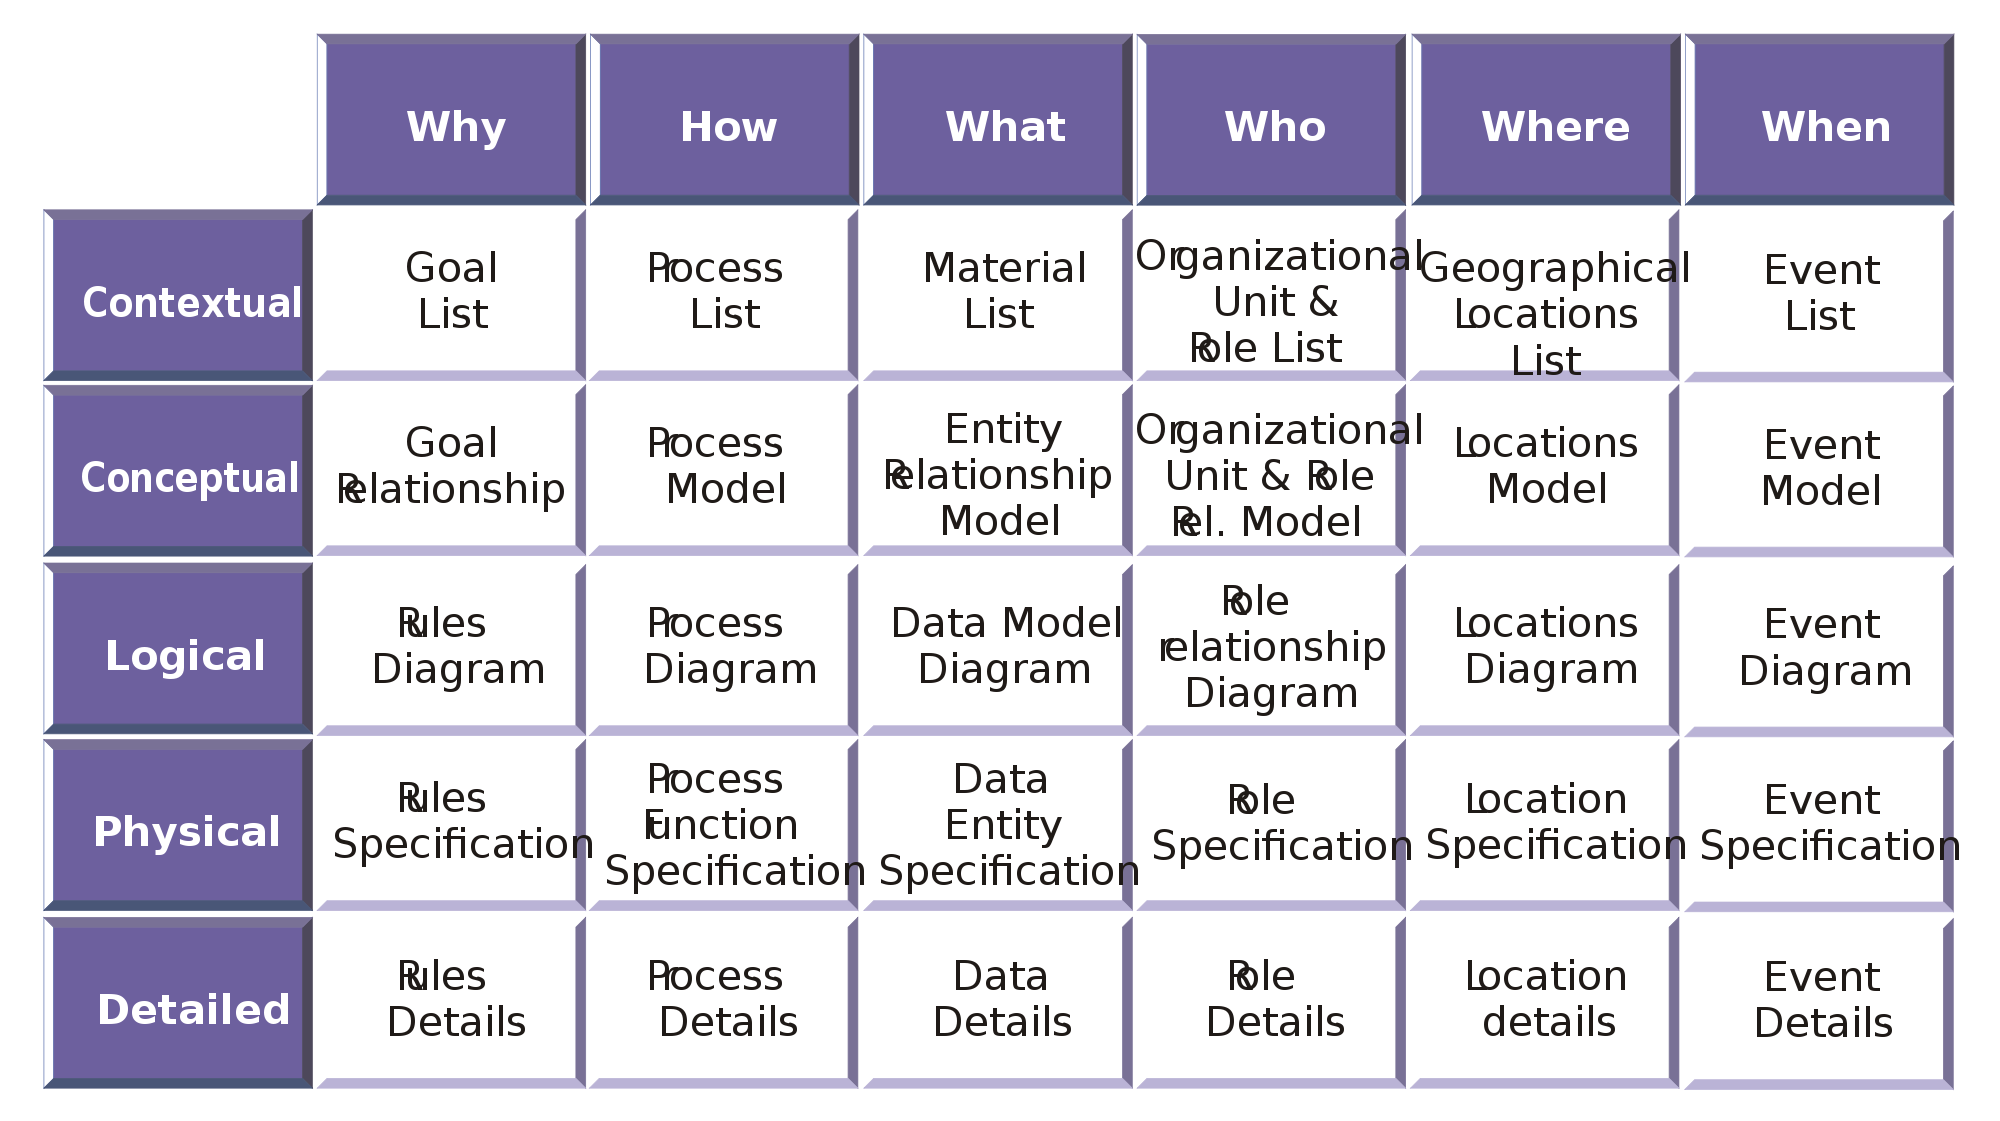
\includegraphics[scale=.3, angle=90, max size={\textwidth}{\textheight}]{ES1}
\caption{Current View of Zachman Framework \cite{ES05}}
\label{ES1}
\end{center}
\end{figure}

\subsection{Focus of Columns}
In summary, each perspective focuses attention on the same fundamental questions, then answers those questions from that viewpoint, creating different descriptive representations (i.e., models), which translate from higher to lower perspectives. The basic model for the focus (or product abstraction) remains constant. The basic model of each column is uniquely defined, yet related across and down the matrix.[26] In addition, the six categories of \gls{EA} components, and the underlying interrogatives that they answer, form the columns of the Zachman Framework and these are:\index{Enterprise Architecture}
\begin{enumerate}
\item The data description — What
\item The function description — How
\item The Network description — Where
\item The people description — Who
\item The time description — When
\item The motivation description — Why
\end{enumerate}
In Zachman’s opinion, the single factor that makes his framework unique is that each element on either axis of the matrix is explicitly distinguishable from all the other elements on that axis. The representations in each cell of the matrix are not merely successive levels of increasing detail, but actually are different representations — different in context, meaning, motivation, and use. Because each of the elements on either axis is explicitly different from the others, it is possible to define precisely what belongs in each cell.
\subsection{Models of Cells}
The kinds of models or architectural descriptive representations are made explicit at the intersections of the rows and columns. An intersection is referred to as a cell. Because a cell is created by the intersection of a perspective and a focus, each is distinctive and unique. Since each cell is distinctive and unique, the contents of the cell are normalized and explicit per the perspectives focus.[26]
The cell descriptions in the table itself uses general language for a specific set of targets. Below the focus of each cell in this particular Zachman Framework is explained:

\subsubsection{Contextual}
\begin{enumerate}
\item (Why) Goal List – primary high level organization goals
\item (How) Process List – list of all known processes
\item (What) Material List – list of all known organizational entities
\item (Who) Organizational Unit and Role List – list of all organization units, sub-units, and identified roles
\item (Where) Geographical Locations List – locations important to organization; can be large and small
\item (When) Event List – list of triggers and cycles important to organization
\end{enumerate}
\subsubsection{Conceptual}
\begin{enumerate}
\item (Why) Goal Relationship Model – identifies hierarchy of goals that support primary goals
\item (How) Process Model – provides process descriptions, input processes, output processes
\item (What) Entity Relationship Model – identifies and describes the organizational materials and their relationships
\item (Who) Organizational Unit and Role Relationship Model – identifies enterprise roles and units and the relationships between them
\item (Where) Locations Model – identifies enterprise locations and the relationships between them
\item (When) Event Model – identifies and describes events and cycles related by time
\end{enumerate}
\subsubsection{Logical}
\begin{enumerate}
\item (Why) Rules Diagram – identifies and describes rules that apply constraints to processes and entities without regard to physical or technical implementation
\item (How) Process Diagram – identifies and describes process transitions expressed as verb-noun phrases without regard to physical or technical implementation
\item (What) Data Model Diagram – identifies and describes entities and their relationships without regard to physical or technical implementation
\item (Who) Role Relationship Diagram – identifies and describes roles and their relations to other roles by types of deliverable without regard to physical or technical implementation
\item (Where) Locations Diagram – identifies and describes locations used to access, manipulate, and transfer entities and processes without regard to physical or technical implementation
\item (When) Event Diagram – identifies and describes events related to each other in sequence, cycles occur within and between events, without regard to physical or technical implementation
\end{enumerate}
\subsubsection{Physical}
\begin{enumerate}
\item (Why) Rules Specification – expressed in a formal language; consists of rule name and structured logic to specify and test rule state
\item (How) Process Function Specification – expressed in a technology specific language, hierarchical process elements are related by process calls
\item (What) Data Entity Specification – expressed in a technology specific format; each entity is defined by name, description, and attributes; shows relationships
\item (Who) Role Specification – expresses roles performing work and workflow components at the work product detailed specification level
\item (Where) Location Specification – expresses the physical infrastructure components and their connections
\item (When) Event Specification – expresses transformations of event states of interest to the enterprise
\end{enumerate}
\subsubsection{Detailed Representation}
Eventually the cells with the detailed representation give Rules detail for (Why); Process detail for (How); Data detail for (What); Role detail for (Who); Location detail for (Where); and Event detail for (When).
There is a sixth row in the current Zachman framework, but it is not used for \gls{EA} while the enterprise is described by rows one to six, \gls{EA} uses only rows one to five, thus only five rows are shown here.
Since the product development (i.e., architectural artifact) in each cell or the problem solution embodied by the cell is the answer to a question from a perspective, typically, the models or descriptions are higher-level depictions or the surface answers of the cell. The refined models or designs supporting that answer are the detailed descriptions within the cell. Decomposition (i.e., drill down to greater levels of detail) takes place within each cell. If a cell is not made explicit (defined), it is implicit (undefined). If it is implicit, the risk of making assumptions about these cells exists. If the assumptions are valid, then time and money are saved. If, however, the assumptions are invalid, it is likely to increase costs and exceed the schedule for implementation.\index{Enterprise Architecture}

\section{SOA Selected Topics}
\subsection{SOA Definition}
\index{Service Oriented Architecture}
\label{SOADefinition}
There is no agreed upon definition for \gls{SOA}.
\begin{itemize}
\item To the chief information officer (CIO), \gls{SOA} is a journey that promises to reduce the lifetime cost of the application portfolio, maximize return on investment (ROI) in both application and technology resources, and reduce lead times in delivering solutions to the business.
\item To the business executive, \gls{SOA} is a set of services that can be exposed to their customers, partners, and other parts of the organization. Business capabilities, function, and business logic can be combined and recombined to serve the needs of the business now and tomorrow. Applications serve the business because they are composed of services that can be quickly modified or redeployed in new business contexts, allowing the business to quickly respond to changing customer needs, business opportunities, and market conditions.
\item To the business analyst, \gls{SOA} is a way of unlocking value, because business processes are no longer locked in application silos. Applications no longer operate as inhibitors to changing business needs.
\item To the chief architect or enterprise architect, \gls{SOA} is a means to create dynamic, highly configurable and collaborative applications built for change. \gls{SOA} reduces IT complexity and rigidity. \gls{SOA} becomes the solution to stop the gradual entropy that makes applications brittle and difficult to change. \gls{SOA} reduces lead times and costs because reduced complexity makes modifying and testing applications easier when they are structured using services.\index{Service Oriented Architecture}
\item To the IT architect, \gls{SOA} is the architectural solution for integrating diverse systems by providing an architectural style that promotes loose coupling and reuse. Many IT architects think they have seen this style before with earlier architectural initiatives such as \gls{DCE}, the Distributed Computing Environment, and \gls{CORBA}, the Common Object Request Broker Architecture.
\item To the developer, \gls{SOA} is a programming model or paradigm where web services and contracts becomes a dominant design for interoperability. It is a web service when it uses a \gls{WSDL} or equivalent specification for describing the service. Web services enable organizations to communicate information, using messages, without intimate knowledge of each others IT systems.
\end{itemize}
\index{Service Oriented Architecture}

\subsection{SOA is an Architectural Style}
\gls{SOA} is often seen as an architectural style that has been around for years. In \gls{SOA} scenario, a service consumer invokes or uses a service. The service consumer uses the service description to obtain necessary information about the provider service (e.g., account service) to be consumed. The service description provides the binding information so the consumer can connect to the service, and the description identifies the various operations (e.g., open or close account) available from the provider service. A broker can be used to find the service using a registry that houses information about the service and its location.\index{Service Oriented Architecture}

\subsection{Fundamental Constructs of SOA}
The most basic construct or building block of \gls{SOA} is a service. Software engineering over the years has evolved from procedural to structured programming to object-oriented programming to component-based development and now to service oriented. There are different levels of abstraction from objects to services. Each evolution of abstraction builds on the previous, and \gls{SOA} embraces the best practices of object and component development. Evolution goes through the following three steps:\index{Service Oriented Architecture}
\begin{itemize}
\item Object is the encapsulation of data and behavior in one data type; class; as depicted in figure \ref{SOA1-1} presented in page \pageref{SOA1-1}. Objects are instances of classes that exist for a certain period of time. Objects communicate with each other via exchanged messages. Messages are instructive, not descriptive. Object based development advances software design by providing more support for hiding behavior and data through objects, however, large number of interconnected objects create dependencies that can be difficult to manage. Object based software development is called Object-Oriented Analysis and Design (OOAD) [90].\index{Service Oriented Architecture}
\begin{figure}
\begin{center}
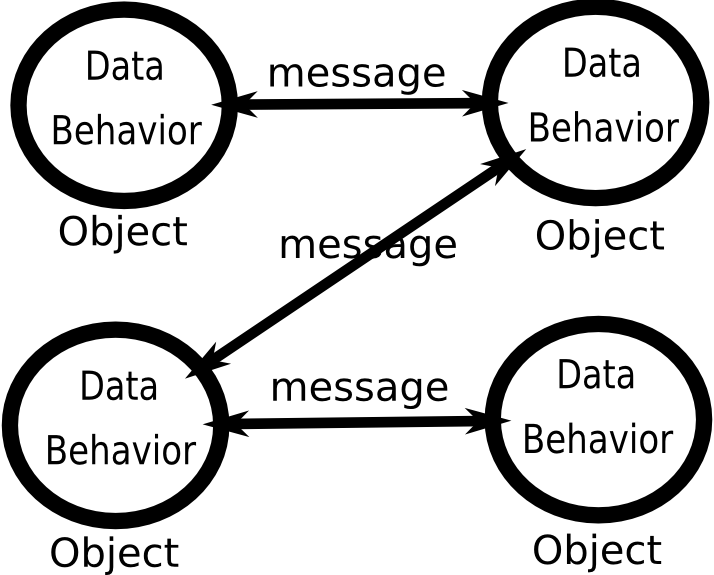
\includegraphics[scale=.5, max size={\textwidth}{\textheight}]{SOA1-1}
\caption{Objects encapsulate data and behavior}
\label{SOA1-1}
\end{center}
\end{figure}
\item Software Components are more sophisticated software modules than objects and require fundamental changes in systems thinking, software processes, and technology utilization. Software component is a unit of composition with contractually specified interfaces and explicit context dependencies [95]. It is a group of objects with has specified interface, working together to provide an application function, such as depicted in figure \ref{SOA1-2} presented in page \pageref{SOA1-2}. Component may refer to many different software constructs, from single application logic to an entire functional system. In all cases, a component is a software package with one or more well defined interfaces. Components overlap the properties of object orientation, such as encapsulation and polymorphism, except it reduces the property of inheritance. In component thinking, inheritance is tightly coupled and unsuitable for most forms of packaging and reuse [96]. Instead, components reuse the functionality by invoking other objects and components rather than inheriting from them [97]. Reusable components are good reflection of effective software design. The development of software architecture based on component specifications supports parallel and independent building of the system parts. Many platform vendors have already produced software infrastructures which support component oriented technology.
\begin{figure}
\begin{center}
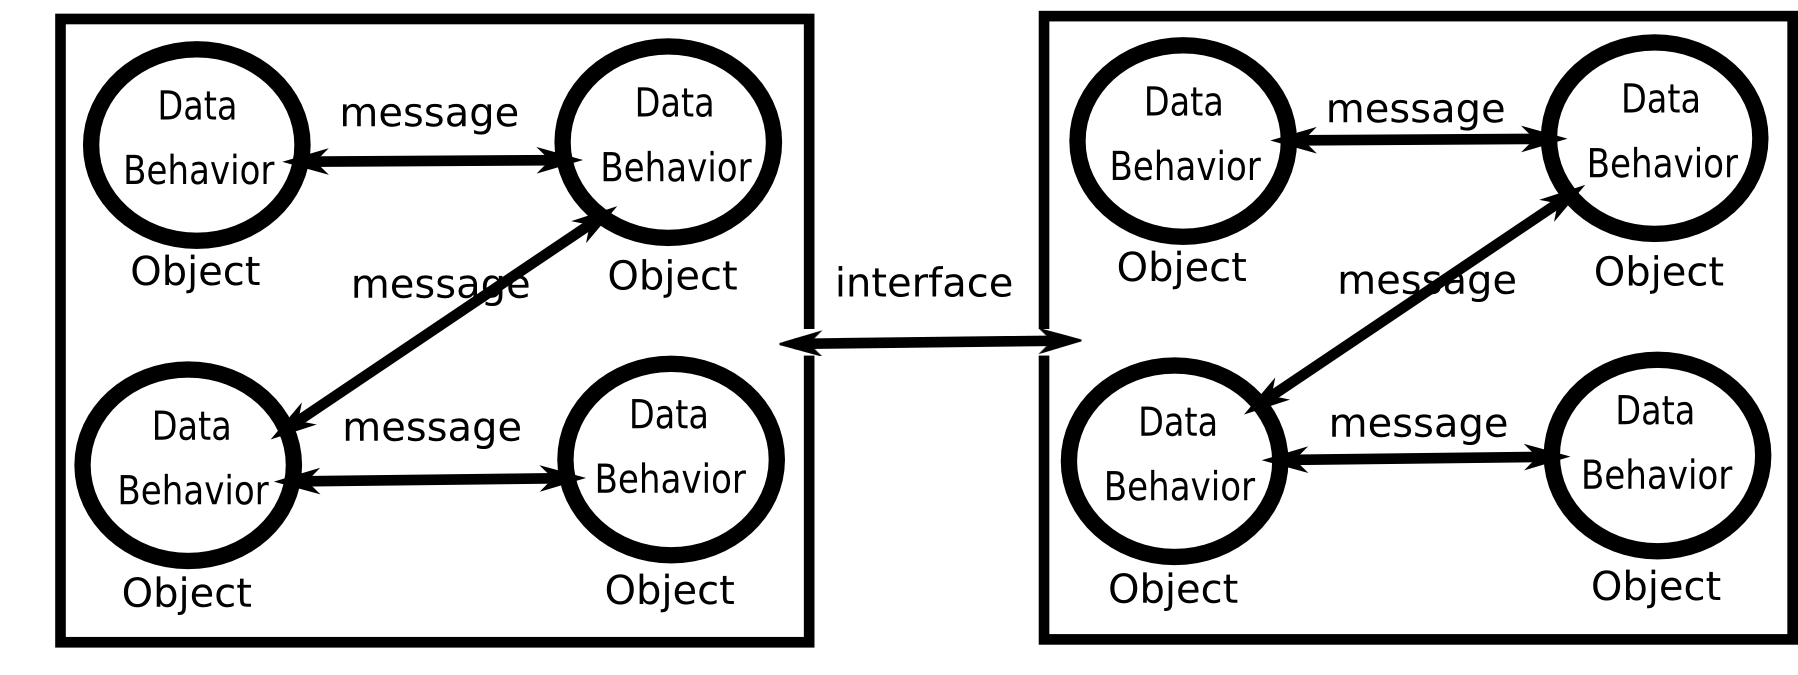
\includegraphics[scale=.3, max size={\textwidth}{\textheight}]{SOA1-2}
\caption{Components encapsulate Objects}
\label{SOA1-2}
\end{center}
\end{figure}
\item Service and Service Models: Service is a component capable of performing a task [98]. Services can be categorized based on the nature of logic they encapsulate and the manner in which they are typically utilized within \gls{SOA} as depicted in [99]. \index{Service Oriented Architecture}
\end{itemize}

\subsection{Service Attributes}
A service in \gls{SOA} is the logical, self-contained business function. Services in \gls{SOA} have the following attributes:
\begin{itemize}
\item \textbf{Stateless:} \gls{SOA} services neither remember the last thing they were asked to do nor do they care what the next is. Services are not dependent on the context or state of other services, only on their functionality. Talking on the telephone is stateful, whereas posting a letter is stateless. The World Wide Web provides an excellent example, where each request from a user for a web page or URL results in the requested pages being served, but without the web server remembering the request later. Each request or communication is discrete and unrelated to requests that precede or follow it.\index{Service Oriented Architecture}
\item \textbf{Discoverable:} A service must be discoverable by potential consumers of the service. After all, if a service is not known to exist, it is unlikely ever to be used. Services are published or exposed by service providers in the \gls{SOA} service directory, from which they are discovered and invoked by service consumers.
\item \textbf{Self-describing:} The \gls{SOA} service interface describes, exposes, and provides an entry point to the service. The interface contains all the information a service consumer needs to discover and connect to the service, without ever requiring the consumer to understand (or even see) the technical implementation details.
\item \textbf{Composable:} \gls{SOA} services are, by nature, composite. They can be composed from other services and, in turn, can be combined with other services to compose new business solutions.
\item \textbf{Loose coupling:} Loose coupling allows the concerns of application features to be separated into independent pieces. This separation of concern provides a mechanism for one service to call another without being tightly bound to it. Separation of concerns is achieved by establishing boundaries, where a boundary is any logical or physical separation that delineates a given set of responsibilities. For example, an account service has open account, authorization, and audit features representing delineations of responsibilities and three separations of concerns.\index{Service Oriented Architecture}
\item \textbf{Governed by policy:} Services are built by contract. Relationships between services (and between services and service domains) are governed by policies and service-level agreements (SLAs), promoting process consistency and reducing complexity.
Independent location, language, and protocol: Services are designed to be location transparent and protocol/platform independent (generally speaking, accessible by any authorized user, on any platform, from any location).
\item \textbf{Coarse-grained:} Services are typically coarse-grained business functions. Granularity is a statement of functional richness for a service—the more coarse-grained a service is, the richer the function offered by the service. Coarse-grained services reduce complexity for system developers by limiting the steps necessary to fulfill a given business function, and they reduce strain on system resources by limiting the chattiness of the electronic conversation. Applications by nature are coarse- grained because they encompass a large set of functionality; the components that comprise applications would be fine-grained. Similarly, within an application, a service such as “get account information” (which returns name, account number, and address) could be described as coarse-grained, whereas a service to “get account number” could be described as fine- grained.
\item \textbf{Asynchronous:} Asynchronous communication is not required of an \gls{SOA} service, but it does increase system scalability through asynchronous behavior and messaging techniques. Unpredictable network latency and high communications costs can slow response times in an \gls{SOA} environment, due to the distributed nature of services. Asynchronous behavior and messaging allow a service to issue a service request and then continue processing until the service provider returns a response.\index{Service Oriented Architecture}
\end{itemize}
\subsection{EAI vs. SOA vs. SOI}
\gls{SOI} uses \gls{SOA} or Web services to integrate applications. It is an evolution from the \gls{EAI}, with the additional innovation of using services and service contracts for integration. This enables the creation of a set of loosely coupled interfaces that can interact with one another to achieve the purposes of integration with greater flexibility. \gls{SOI} is a subset of \gls{SOA} (although some see \gls{SOI} and \gls{SOA} as different, when in fact \gls{SOA} is broad and accommodates a wide range of adoption scenarios). This range accommodates different levels of maturity, and the range of adoptions produces different business outcomes. That is, some organizations use only \gls{SOA} centers for integration and don’t seek other strategic benefits of \gls{SOA}. \gls{SOI} adoption may or may not use an enterprise service bus (ESB) because \gls{SOI} is simply the adoption and use of services for integration. The utility of distinguishing \gls{SOI} and \gls{SOA} is not particularly useful unless \gls{SOI} is used to describe specific integration patterns or is defined in a manner that provides some unique utility for software engineering. \gls{EAI} integrates applications and systems using middleware. \gls{EAI} solutions are technology based but often not based on standards such as Web services. This is a primary difference between \gls{EAI} solutions and \gls{SOA}. Although \gls{SOA} builds on \gls{EAI} for integration, it also offers improvements, largely in the use of services. \gls{SOA} introduces a higher abstraction level than \gls{EAI} by using services and service contracts. \gls{EAI} typically uses application programming interfaces (APIs), and \gls{SOA} uses service interfaces and contracts.\index{Service Oriented Architecture}
\gls{EAI} has two main integration patterns: hub and spoke and publish-subscribe. In the hub-and-spoke pattern, an application informs the broker of an event (e.g., a \gls{DB} create, read, update, or delete action performed in the application). The broker takes care of transforming the message, routing the message, and triggering the right action on the client applications. The broker will know, based on internal logic, which client applications to invoke. In the publish-subscribe pattern, the “provider” application publishes events to the middleware, and “client” applications subscribe to these events based on filtering rules. The middleware on a published event will send the transformed message to the subscribing applications.
Another difference between \gls{EAI} and \gls{SOA} is that in \gls{EAI}, often, no direct relation exists between requester and provider applications, whereas in \gls{SOA} there does. In \gls{EAI}, applications inform the middleware of some event that took place, but they are ignorant about what happens next. It is the responsibility of the middleware to transform and route the message. In an \gls{SOA} solution, a client application (the service consumer) calls a service, which is mediated through an ESB, on to the service-providing application. Of course, \gls{EAI} solutions using messaging middleware could be programmed differently to have such awareness.\index{Service Oriented Architecture}
\subsection{Building Blocks of an SOA Infrastructure}
\index{Service Oriented Architecture}
The building blocks of an \gls{SOA} infrastructure should address the underlying technical infrastructure components needed to support the layers (Consumers; Business Processes; Services; Service Components; Governance; Data Architecture; Quality of Service, Security, Management, Monitoring; and Integration).
In identifying the \gls{SOA} infrastructure components, Figure \ref{InfraSOA} presented in page \pageref{InfraSOA} separates the building blocks into three categories (consumer, functional, and operational) to provide an abstraction that can be used for consistency and reuse across platforms within an organization. That is, engineers (enterprise or infrastructure architects) can use this model as a basis for determining the necessary software products or technologies necessary to provision that building block.\index{Service Oriented Architecture}
\begin{figure}
\begin{center}
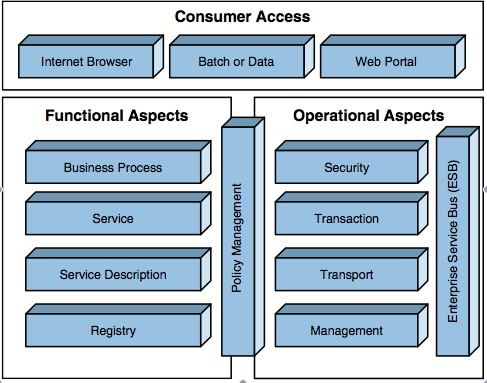
\includegraphics[scale=.8, max size={\textwidth}{\textheight}]{InfraSOA}
\caption{Infrastructure SOA Building Blocks \cite{100SOA}}
\end{center}
\label{InfraSOA}
\end{figure}
\subsection{SOA Role in Embedded or Real-Time Systems}
\index{Service Oriented Architecture}
Embedded or real-time systems require a high degree of availability, performance, and response time. Often, embedded systems are responsible for monitoring the health of humans, machines, or services. The role of \gls{SOA} is akin to its role in providing context-aware services that can be leveraged by embedded or real-time systems. However, the implementation of these systems must address the most stringent performance requirements in latency, availability, and throughout. Therefore, current Web services technologies, for example, might not be suitable for the implementation of such services. There is a class of loosely coupled service implementations that go beyond Web services implementations. They are inspired by \gls{SOA} service interfaces and loose coupling, and they will be applied to embedded or real-time systems that use mobile robotics and real- time systems that use sensors and actuators within a real-time context.
\subsection{SOA vs. EDA}
\index{Service Oriented Architecture}
EDA and \gls{SOA} are complementary in that \gls{SOA} allows all the interaction patterns prescribed by EDA and services to be event driven. However, distinct differences exist in the architectural building blocks to support EDA and its interaction patterns. Optimal \gls{SOA} implementations do not exclusively apply the request-reply interaction pattern, although there may be instances where this is the optimal architectural decision. EDA consists of a set of constructs (runtime artifacts, tools, application programming interfaces) intended to support event-driven behavior. Event-driven behavior can be part of a service design where application logic execution is invoked directly or indirectly because an event has occurred. Perhaps one big difference between EDA and \gls{SOA} is that the various interaction patterns are designed as services and applications with EDA, whereas with \gls{SOA}, it’s provided externally through the use of ESB, registry patterns, and implementations.


\section{Summary}
Today, organizations use computer-based \gls{IS} to better manage operations in the digital world. These organizations use information systems to provide high-quality goods and services as well as to gain or sustain competitive advantage over rivals. In addition to helping organizations to be competitive, information systems have contributed to tremendous societal changes. An \gls{IS} can be defined technically as a set of interrelated components that collect (or retrieve), process, store, and distribute information to support decision making and control in an organization. In addition to supporting decision making, coordination, and control, information systems may also help managers and workers analyze problems, visualize complex subjects, and create new products \cite{MIS-DigitalFirm}. \gls{IS} contain information about significant people, places, and things within the organization or in the environment surrounding it. By information we mean data that have been shaped into a form that is meaningful and useful to human beings. Data, in contrast, are streams of raw facts representing events occurring in organizations or the physical environment before they have been organized and arranged into a form that people can understand and use. 

This chapter presented different roles of \gls{IS} as we move into the digital world and how they have helped fuel decision making. We then highlight what information systems are, how \gls{DSS} have evolved to become a vital part of modern organizations, what are the main technologies behind \gls{DSS}, and why this understanding is necessary to become an effective manager in the digital world. Chapter concludes by discussing \gls{EA}, its components, and different examples of \textit{defacto} standards.\index{Enterprise Architecture}

\section{Review Questions}
\begin{enumerate}
\item Give a definition of each of the following:
\begin{itemize}
\item Information System
\item Management Support System
\item Enterprise Information System
\item Group Support System
\item Knowledge Management System \index{Knowledge Management System}
\item Expert Systems
\item Hybrid Support Systems
\item Enterprise Architecture
\end{itemize}
\item Enterprise Architecture is a fundamental model of thinking about Organizations' architectures. Given that information, answer the following:
\begin{itemize}
\item What is the main difference between Enterprise and Organization?
\item TOGAF, and Zachman are different \gls{EA} Frameworks. List and describe the different components of each.
\item What is the role of ArchiMate in Enterprise Architecture?
\end{itemize}
\item What is SOA?
\item What are the Fundamental Constructs of SOA?
\item What is SOA Role in Embedded Systems?
\end{enumerate}

\section{Exercises and Labs}
In Labs, you shall be getting familiar with Java programming language, as it is the programming language we will be using to build, deploy, and consume different online Webservices and \gls{SOA} systems presented in this book.

\chapter{SW Architecture and Integration}
\label{SWArchitectureandIntegration}
\section{Introduction}
It has become accepted that there is a clear need for an ‘architectural view’ of systems \cite{M01}. \gls{EA}s that satisfies nowadays enterprises’ requirements should be presented. Software architecture is one class of \gls{EA} that should address organizational requirements like systems interoperability, integration, agility, and other requirements \cite{W26,M03}. The architectural view of systems (both business and IT systems) is defined in \gls{ANSI/IEEE} standard 1471-2000 as “the fundamental organization of a system, embodied in its components, their relationships to each other and the environment, and the principles governing its design and evolution”. Enterprises can be thought of as the combination of business needs, and IT capabilities. Agile organizations are those where IT serves business needs, not limiting it \cite{M04}.\index{Enterprise Architecture}
\subsection{Enterprise Architecture Dimensions}
Different dimensions of the enterprise need to be defined in order to generate the \gls{EA}. From enterprise point of view, architectures are classified into four categories \cite{W26}: Business Architecture, Information Technology (IT) Architecture, Information Architecture, Application (software) Architecture as depicted in figure \ref{M1} presented in \pageref{M1}. \gls{EA} tends to define the enterprise from the four dimensions in order to connect between them and present a complete view for the enterprise.\index{Enterprise Architecture}

\begin{figure}
\begin{center}
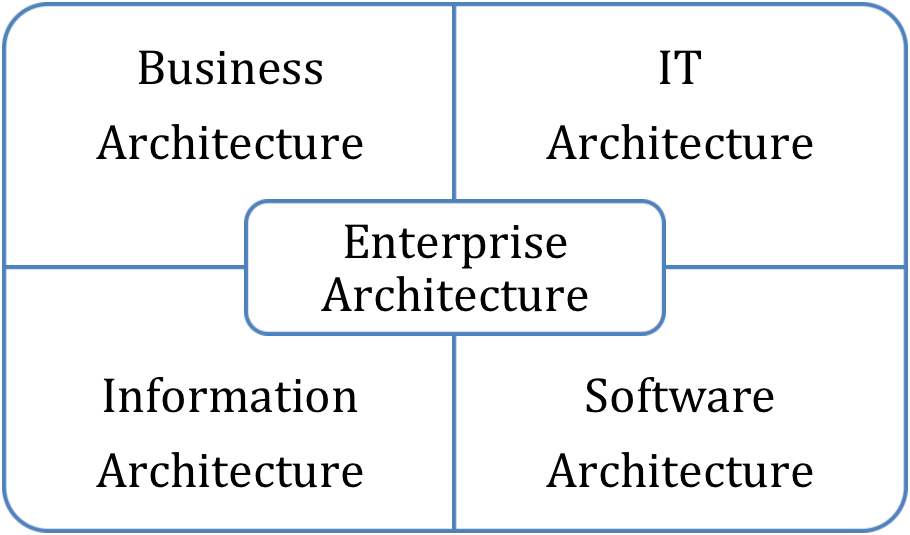
\includegraphics[scale=.8, max size={\textwidth}{\textheight}]{M1}
\caption{\gls{EA} Dimensions}
\end{center}
\label{M1}
\end{figure}

\subsection{Business Architecture}
A business or business process architecture defines the business strategy, governance, organization, and key business processes within an enterprise. The fields of Business Process Reengineering (BPR) and \gls{BPM} focus on the analysis and design of business processes, not necessarily represented in an IT system \cite{W26}. Business Architecture defines the business roadmap usually via defining the business processes \cite{M05}.
\subsubsection{IT Architecture}
The IT architecture defines the hardware and software building blocks that make up the overall \gls{IS} of the organization \cite{W26}. IT architecture includes hardware and software infrastructure including \gls{DB} and middleware technologies. The IT architecture should enable achievement of the business goals using a software infrastructure that supports the procurement, development, and deployment of core mission-critical business applications. The purpose of the IT architecture is to enable a company to manage its IT investment in a way that meets its business needs by providing a foundation upon which data and application architectures can be built.
\subsubsection{Information Architecture}
The data architecture of an organization includes logical and physical data assets and data management resources. Information is becoming one of the most important assets a company has in achieving its objectives, and the IT architecture must support it. Information Architecture spans Business and IT Architectures, brings them together, keeps them together, and provides the necessary rich contextual environment to solve the ubiquitous data-quality problem \cite{M06}.
\subsubsection{Software Architecture}
Application architecture serves as the blueprint for individual application systems, their interactions, and their relationships to the business processes of the organization. A software application is a computer program or set of programs that uses existing technologies to solve some end-user problem such as the automation of an existing business process. Software architecture can be defined as “the sum of the nontrivial modules, processes, and data of the system, their structure and exact relationships to each other, how they can be and are expected to be extended and modified, and on which technologies they depend, from which one can deduce the exact capabilities and flexibility of the system, and from which one can form a plan for the implementation or modification of the system” \cite{M07}. Application Architecture defines the form and function of the applications that will be developed to deliver the required functionality of the system \cite{M01}.
\gls{EA} classes utilize each other, and build over each other. Distinctions between classes are blurred because they all serve each other, and serve the enterprise. \gls{EA} classes’ utilization can be thought of as depicted in figure \ref{M2} presented in page \pageref{M2}. Common software architectures are presented in order to address the architecture that might solve most well known software architecture limitations; like lack of scalability, integration, and interoperability with different \gls{IS}. From this point on, Software Architecture and Architecture will be used interchangeably to refer to Software Architecture.\index{Enterprise Architecture}

\begin{figure}
\begin{center}
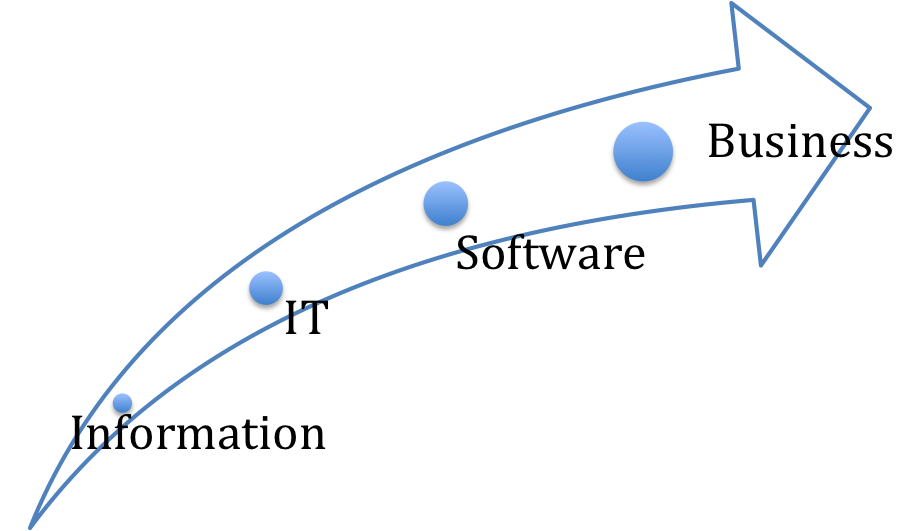
\includegraphics[scale=.7, max size={\textwidth}{\textheight}]{M2}
\caption{Enterprise Architecture Classes Utilization}
\end{center}
\label{M2}
\end{figure}

\index{Enterprise Architecture}
This chapter goes as follows: Section Two presents the relation between Software Architecture and Systems’ Non-Functional Requirements. Section Three discusses the importance of Software Architecture. Section Four lists the most common Software Architecture Patterns while in Section Five authors present “Integration” as the selected criteria for comparing between different patterns. Section Six maps the different integration techniques and different Software Architecture Patterns; highlighting the driving and restraining forces for utilizing each one. Summary is presented in Section Seven with a proposed map between different integration techniques and software architecture patterns. 

\section{SW Architecture and System Design}
There are aspects that should be designed within any system. Those aspects are: Architecture, Functionality, and Presentation as depicted in figure \ref{M3} presented in page \pageref{M3}. System design include: Architecturally defining subsystems and their functions, defining interface(s) for each subsystem and determining how those subsystems will interact, and allocating those subsystems to different components, as defined in \cite{EV10}. 

\begin{figure}
\begin{center}
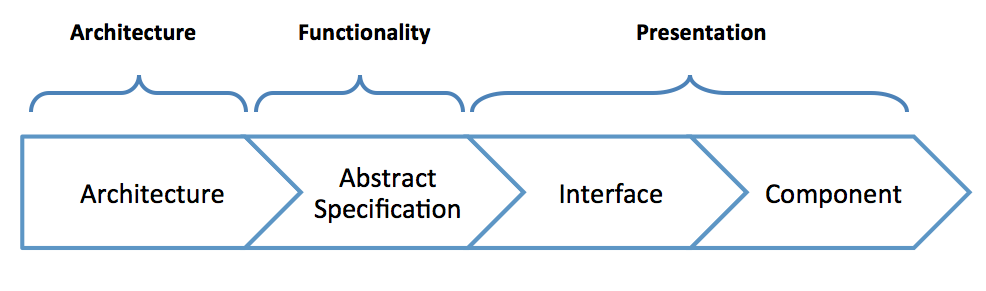
\includegraphics[scale=.4, max size={\textwidth}{\textheight}]{M3}
\caption{Architecture Design is one aspect of System Design}
\end{center}
\label{M3}
\end{figure}

Each of System Design’s steps includes one or more functionality. Functionality can be mapped to system design steps as follows:
\begin{enumerate}
\item Architectural Design: includes identifying and documenting sub-systems making the system and their relationships.
\item 	Abstract Specification: includes producing an abstract specification of each sub-systems services and the constraints under which it must operate.
\item 	Interface Design: includes defining each subsystems interface with other sub-systems is designed and documented.
\item 	Component Design: includes allocating services to different components and designing interfaces of these components.
\end{enumerate}

Architecture is one aspect of a system to be designed, as well as the presentation of information and the functionality of the system. System requirements are either functional or non-functional \cite{M07}. Functional requirements are statements of services that systems should provide. Non-functional requirements present requirements that arose as a result of functional requirements. Architecture design is one step of systems design that shall satisfy non-functional requirements as it satisfies functional requirements \cite{W26}. Some of the non-functional requirements that shall be satisfied by architectural design are presented in figure \ref{M4} presented in page \pageref{M4}.

\begin{figure}
\begin{center}
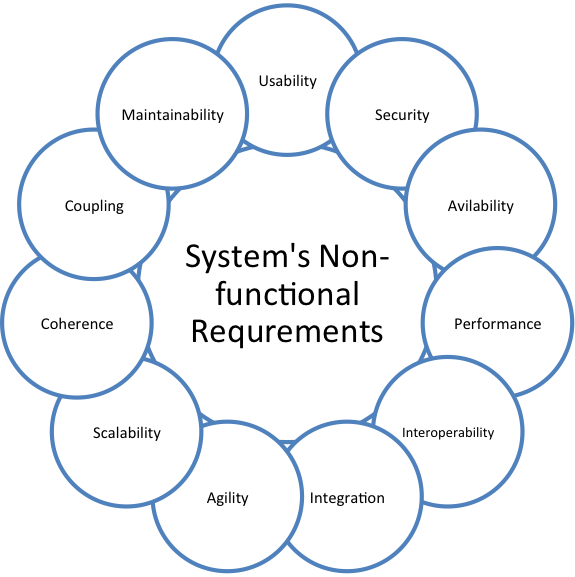
\includegraphics[scale=1.5, max size={\textwidth}{\textheight}]{M4}
\caption{Systems non-functional requirements}
\label{M4}
\end{center}
\end{figure}

\section{Importance of SW Architecture}
\gls{SW} architecture matters because a good one is a key element to success \cite{M07}. Though the fact that Systems have architectures but architectures are not systems \cite{W26} does not decrease architectures effects on systems. Some of the ways that software architecture influences success are \cite{M07}:
\begin{itemize}
\item Longevity: It is important to take time defining a good architecture because Architectures live longer than teams created them expects.
\item Stability: Architectural stability helps ensure a minimum of fundamental rework as the system's functionality is extended over multiple release cycles, thus reducing total implementation costs.
\item Degree and Nature of Change: Architecture determines the nature of change within the system. Some changes are perceived as applicable; others are perceived as not applicable.
\item Profitability: Profitable architecture is the sustainable architecture within an acceptable cost.
\item Social Structure: Architectures helps strengthening and weakening the social structure of the team. Teams can make social benefits form architectures during project time.
\item Boundaries Defined: During the architectural design process the team makes numerous decisions about what is "in" or "out of" the system. These boundaries, and the manner in which they are created and managed, are vital to the architecture's ultimate success.
\end{itemize}

\subsection{Distributed Approach Advantages}
Advantages of using a distributed approach to systems development \cite{SWE9}:
\begin{enumerate}
\item Resource sharing A distributed system allows the sharing of hardware and software resources—such as disks, printers, files, and compilers—that are associated with computers on a network.
\item Openness Distributed systems are normally open systems, which means that they are designed around standard protocols that allow equipment and software from different vendors to be combined.
\item Concurrency In a distributed system, several processes may operate at the same time on separate computers on the network. These processes may (but need not) communicate with each other during their normal operation.
\item Scalability In principle at least, distributed systems are scalable in that the capabilities of the system can be increased by adding new resources to cope with new demands on the system. In practice, the network linking the individual computers in the system may limit the system scalability.
\item Fault tolerance The availability of several computers and the potential for replicating information means that distributed systems can be tolerant of some hardware and software failures. In most distributed systems, a degraded service can be provided when failures occur; complete loss of service only occurs when there is a network failure.
\end{enumerate}

\section{Common SW Architecture Patterns}
As we seek to handle complexity in building software systems, we encounter various architectural styles better suited to solving a certain class of problems. For example, pipes and filters, blackboard architectures, layered architectures, and so on all have been used to solve specific problems in specific domains. However, other architectural styles provide a greater degree of general utility. In other words, the use of that architectural style is not necessarily limited to solving specific problems within specific domains. Instead, foundation elements of the solutions provided by that architectural style find their way into the foundations of software architecture, rather than being confined to alleviating problems in a specific domain. When developing software systems, service- oriented thinking pushes the boundaries of traditional software architecture and provides new insights into handling complexity, thus deriving commonality and increasing agility. An Architecture Pattern expresses a fundamental structural organization or schema for software systems. It provides a set of predefined subsystems, specifies their responsibilities, and includes rules and guidelines for organizing the relationships between them \cite{M09}. Software architecture patterns can be divided into two categories: Data flow and Control flow \cite{M07,M10}. Data Flow category focuses on functional modules and data transfers, while Control Flow category describes the way control is passed from one part of the system to the other. Data flow software architecture patterns include:
\begin{itemize}
\item Model-View-Controller
\item Presentation-Abstraction-Control
\item Pipe-And-Filter
\item Layered Systems
\item Microkernel
\item Client-Server
\item N-Tier
\item Repository
\item Blackboard
\item Finite State Machine
\item Process Control
\item Multi Agent System
\item \gls{SOA} \index{Service Oriented Architecture}
\item Master-Slave
\item Interpreter
\item Message Broker
\item Message Bus
\item Structural Model
\item Peer-to-peer
\end{itemize}

On the other hand, control flow software architecture patterns include:
\begin{itemize}
\item Call And Return a.k.a. Main program And Subroutines
\item Implicit Invocation a.k.a. Event Based
\item Manager Model
\item Emulated Parallel
\end{itemize}


\section{Non-Functional Requirements}
Shortages, limitations, and deficiencies of \gls{IS} that include lack of agility support and limitations of integration and interoperability are two of the non-functional requirements category. Integration is the main challenge with institutions, and it will be tested against the mentioned software architectures as an indicator for the architecture satisfaction of non-functional requirements.

\subsection{Design Issues of Distributed Systems}
Some of the most important design issues that have to be considered in distributed systems engineering are \cite{SWE9}:
\begin{enumerate}
\item \textbf{Transparency} To what extent should the distributed system appear to the user as a single system? When it is useful for users to understand that the system is distributed?
\item \textbf{Openness} Should a system be designed using standard protocols that support interoperability or should more specialized protocols be used that restrict the freedom of the designer?
\item \textbf{Scalability} How can the system be constructed so that it is scaleable? That is, how can the overall system be designed so that its capacity can be increased in response to increasing demands made on the system?
\item \textbf{Security} How can usable security policies be defined and implemented that apply across a set of independently managed systems?
\item Quality of service How should the quality of service that is delivered to system users be specified and how should the system be implemented to deliver an acceptable quality of service to all users?
\item Failure management How can system failures be detected, contained (so that they have minimal effects on other components in the system), and repaired?
\end{enumerate}

\subsection{Integration}
Application integration is a strategic approach to binding many \gls{IS} together \cite{M30}. The need to integrate applications has been a requirement since business process automation was presented \cite{M31}. Application integration can be one of the forms: Internal Application Integration, External Application Integration, or \gls{EAI} \cite{M32}. Internal application integration techniques integrate organizational applications with each other, while external application integration techniques consider integrating organizational applications with applications outside organizational boundaries. \gls{EAI} platforms centrally integrate heterogeneous system landscapes on process, method and data level \cite{M33}. Internal and External Application Integration present traditional integration levels, where \gls{EAI} presents recent integration levels. Figure \ref{M5} presented in page \pageref{M5} depicts different integration levels as presented in \cite{M31}.

\begin{figure}
\begin{center}
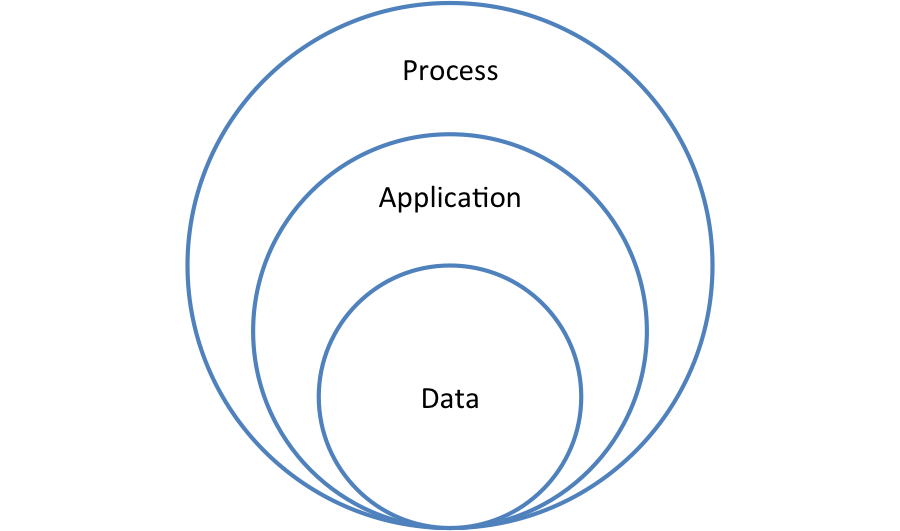
\includegraphics[scale=.7, max size={\textwidth}{\textheight}]{M5}
\caption{Integration Levels}
\label{M5}
\end{center}
\end{figure}

Data level integration allows data to be shared among applications without sharing its application logic. Application level integration integrates applications by getting both connected applications logic aware and enablers of exchanging data. Process level integration presents a new level of integrating applications where integration here facilitates or presents a new business processes.

\section{SW Architectures and Integration Techniques}
Integration is one of the addressed problems that requires picking suitable software architecture as a solution. The agile organization is more extensively integrated than previous organizational forms \cite{M34}, and we need to have agile institutions. Considering how architecture works, advantages and shortages of the architecture, there are architectures that can overcome integration obstacles, and others cannot. There are many integration options that include File Transfer, Shared \gls{DB}, and Messaging \cite{M35}. Considering integration techniques defined in \cite{M36}, there are three common system integration techniques:

\begin{enumerate}
\item Enterprise Wide Standards
\begin{itemize}
\item Standard Data Element Definition
\item Standard Enterprise Wide software
\end{itemize}
\item Middleware
\begin{itemize}
\item TP, \gls{RPC}, MOM, \gls{CORBA}, DCOM,.. .
\item Web services
\end{itemize}
\item Additional Components
\begin{itemize}
\item \gls{DW}
\item Application Routers
\end{itemize}
\end{enumerate}

Figure \cite{M06} presented in page \pageref{M6} depicts a reorder of those integration techniques to be categorized in either one of two categories: Data or Software. Each category satisfies an integration level. Data oriented integration techniques satisfy Data level integration, and Software integration techniques satisfy Application level integration. Each integration technique has driving and restraining forces. Driving forces are forces that push software architects towards using the mentioned technique and supporting software architectures. Restraining forces are forces that push software architects not to use the mentioned technique and supporting architectures.

\begin{figure}
\begin{center}
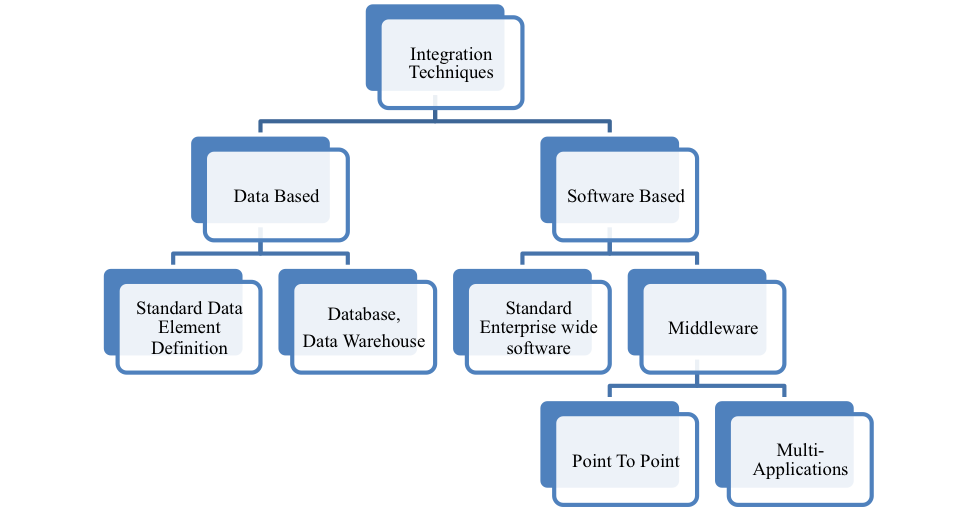
\includegraphics[scale=1, max size={\textwidth}{\textheight}]{M6}
\caption{Integration Techniques}
\label{M6}
\end{center}
\end{figure}

\subsection{Data Based Integration Techniques}
Those are techniques that relies on databases to present integration either by presenting unified standard data element definition, so all applications within the organization can share same data, or by presenting databases, and data warehouses as the organizational repository, and all running applications share same data repository.  By using either technique method, applications are integrated; unfortunately; only on \gls{DB} level. Several restraining forces against this technique are presented in the coming two sections.
\subsubsection{Adopting Standard Data Element Definition}
Custom software uses the same data element definitions as all other software within the system. Thus, uniqueness in syntax and semantics are presented. One of the Software Architectures that fits this technique is: Pipe-And-Filter software architecture. 
\begin{itemize}
\item \textbf{Pipe and Filter Architecture:} A very simple, yet powerful architecture, that is also very robust. It consists of any number of components (filters) that transform or filter data, before passing it on via connectors (pipes) to other components. The filters are all working at the same time. The architecture is often used as a simple sequence, but it may also be used for very complex structures. Figure \ref{M7} presented in page \pageref{M7} depicts mechanism of action of this software architecture \cite{EV10,M10}.
\end{itemize}

\begin{figure}
\begin{center}
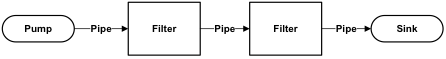
\includegraphics[scale=1, max size={\textwidth}{\textheight}]{M7}
\caption{Pipe-And-Filter Architecture}
\label{M7}
\end{center}
\end{figure}

Components of this architecture are:
\begin{itemize}
\item Pump: or producer is the data source. It can be a static text file, or a keyboard input device, continuously creating new data, or data of another application.
\item Pipe: is the connector that passes data from one filter to the next. It is a directional stream of data that is usually implemented by a data buffer to store all data, until the next filter has time to process it.
\item Filter: transforms or filters the data it receives via the pipes with which it is connected. A filter can have any number of input pipes and any number of output pipes. 
\item Sink: or consumer is the data target. It can be another file, a \gls{DB}, computer screen, or another application. 
\end{itemize}

Applications share same standard data element definition, so, they can pipe data easily among them. By doing so, applications are integrated on data basis. Table  \ref{MT2} presented in page \pageref{MT2} shows Driving and Restraining forces of Adopting Standard Data Element Definition as an integration technique, which unfortunately makes adopting databases and data warehouses not the perfect solution for process level integration. Figure \ref{StandardDataElement} presented in page \pageref{StandardDataElement} presents another view of the driving and restraining forces.

\begin{table}
\begin{center}
\caption{Adopting Standard Data Element Definition Pitfalls}
\begin{tabularx}{\textwidth}{|X|X|}
\hline Driving Forces & Restraining Forces \\
\hline Easier exchange o f data & Costs to develop standards definitions \\
\hline Reduced development time & Costs to change existing systems \\
\hline Reduced maintenance costs & Existing data definitions are different \\
\hline & Some definitions need to be different \\
\hline & Products use different data definitions \\
\hline & Lack of industry standard definitions \\
\hline & Mergers and acquisitions \\
\hline
\end{tabularx}
\end{center}
\label{MT2}
\end{table}

\begin{figure}
\begin{center}
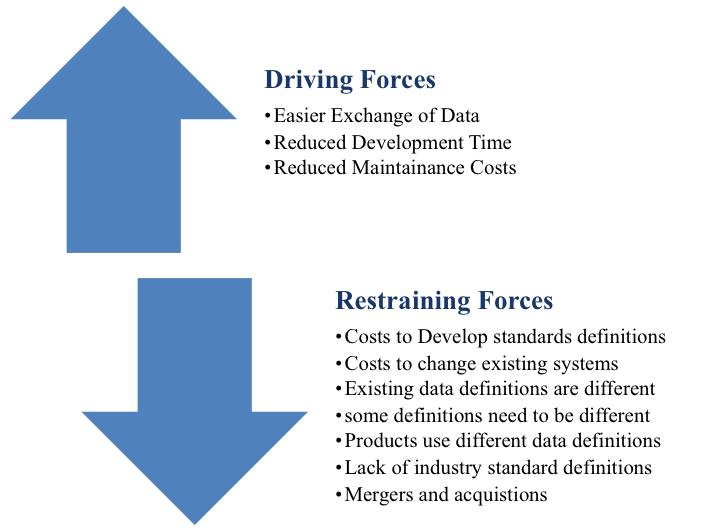
\includegraphics[scale=1, max size={\textwidth}{\textheight}]{StandardDataElement}
\caption{Adopting Standard Data Element Definition Pitfalls}
\label{StandardDataElement}
\end{center}
\end{figure}

\subsubsection{Adopting DB and DW}
\gls{DB} is a collection of persistent data \footnote{Persistent Data are data that once accepted by \gls{DBMS} for entry, can subsequently be removed only by some explicit request to \gls{DBMS}.} that is used by the application systems of some given enterprise \footnote{Enterprise is simply a convenient generic term for any reasonably self-contained commercial, scientific, technical or other organization.}. Databases have too many advantages and they play an important role in today organizations. Benefits of data approach include sharing of data, and reducing redundancy \cite{M37}.  Databases allow data to be shared, that means existing and new applications can share the data in the \gls{DB}. Databases reduce data redundancy by eliminating, or at least controlling redundancy. \gls{DW} is the subject-oriented, integrated, nonvolatile \footnote{Nonvolatile means that, once inserted, data cannot be changed, though it might be deleted.}, time variant data store in support of management's decisions \cite{M38, M39}. \gls{DW} can be thought of as a collection of data from more than one data source (data sources include databases) for providing a single, quiet large repository for the entire organization. Databases and data warehouses have been widely used to integrate applications within organizations. Typical \gls{DW} can be found in \cite{M40}. One of the Software Architectures that fits this technique is: Repository software architecture.
\paragraph{Repository Software Architecture} The repository contains a single data structure, the Repository, and a number of modules called Knowledge Sources, that modify this data structure. These are the only characteristics of repository architecture \cite{EV10,M10}. Figure \ref{M8} presented in page \pageref{M8} depicts how repository architecture behaves.

\begin{figure}
\begin{center}
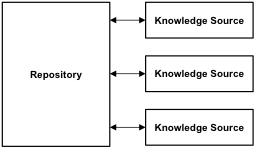
\includegraphics[scale=1, max size={\textwidth}{\textheight}]{M8}
\caption{Repository Architecture}
\label{M8}
\end{center}
\end{figure}

Table \ref{MT3} presented in page \pageref{MT3} depicts the driving and restraining forces of adopting databases and data warehouses as an integration solution, which unfortunately makes adopting databases and data warehouses not the perfect solution for process level integration. Unfortunately, there are restraining forces that make adopting databases and data warehouses not the perfect solution for internal and external organizational applications integration. Figure \ref{DataWarehouse} presented in page \pageref{DataWarehouse} depicts another view of adopting databases and data warehouses pitfalls.

\begin{table}
\begin{center}
\caption{Adopting Databases and Data warehouses Pitfalls}
\begin{tabularx}{\textwidth}{|X|X|}
\hline Driving Forces & Restraining Forces \\
\hline Easier access to enterprise wide data & Costs of development \\
\hline Reduced development time & Different semantics in data sources \\
\hline Reduced maintenance costs	& Semantic translation \\
\hline Minimal effect on operational system & Lack of industry standard definitions \\
\hline Usage of \gls{BI} software	& Deciding what data to warehouse \\
\hline & Delays in getting data to warehouse \\
\hline & Redundancy of data \\ 
\hline & Data quality issues \\
\hline & Brittleness of fixed record exchanges \\
\hline & Performance tuning \\
\hline
\end{tabularx}
\end{center}
\label{MT3}
\end{table}

\begin{figure}
\begin{center}
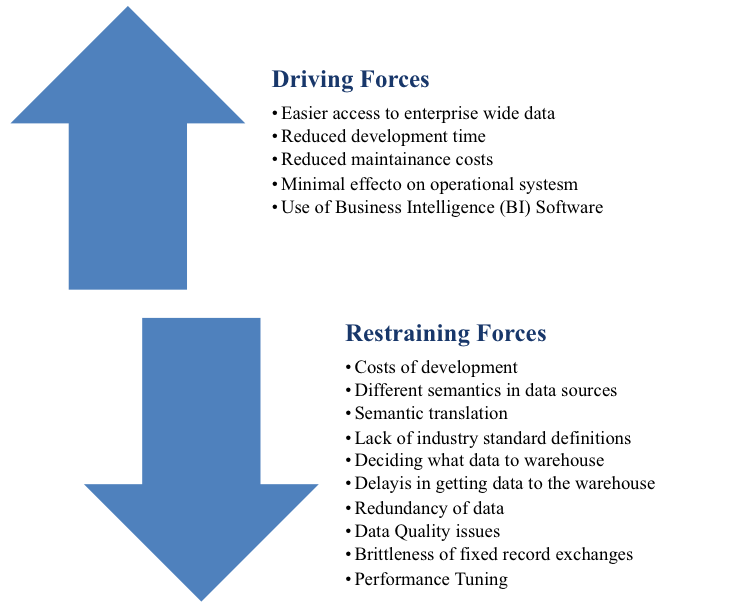
\includegraphics[scale=1, max size={\textwidth}{\textheight}]{DataWarehouse}
\caption{Adopting Databases and Data warehouses Pitfalls}
\label{DataWarehouse}
\end{center}
\end{figure}



\subsection{SW Based Integration Techniques}
Another integration technique presented is the one based on using software as the orientation of integration solution. Either using standard enterprise wide software or presenting middleware is a software oriented solutions.
\subsubsection{Standard Enterprise Wide Software}
This means that whole organization uses the same software; this means that the whole organization is using the same data definitions, semantics, and formats for exchanging data. \gls{ERP} presents this technique as a solution to whole enterprise integration solution. \gls{ERP} integrates \gls{SCM} System, Enterprise Management System, \gls{CRM}, e-commerce \cite{M41, M42, M43}. \gls{ERP} providers list include Oracle \cite{M44}, and SAP \cite{M45}. To provide a unified solution to the enterprise, layered architecture is required to enable integration of applications in different aspects. Software Architectures that fit this technique include: Layered Systems, Client-Server, and N-tier architecture.
\begin{itemize}
\item \textbf{Layered Systems:} Layered Systems use layers to separate different units of functionality. Each layer only communicates with the layer above and the layer below. Each layer uses the layer below to perform its function. Communication happens through predefined, fixed interfaces.  A Layer is a design construct. It is implemented by any number of classes or modules that behave like they are all in the same layer. That means that they only communicate with classes in layers immediately above or below their layer and with themselves. Figure \ref{M9} presented in page \pageref{M9} depicts layered systems architecture \cite{M10}. Each layer offers its own kind of functionality. A higher layer uses its lower layer to perform its function. It requires its lower layer. It is possible to define multiple layers at the same level. The user calls a function on an object in the upper layer. This object calls functions in the layer below. These functions in turn approach the layer below and the layer above. The primary disadvantage of layered systems is that they add overhead and latency to the processing of data, reducing user-perceived performance \cite{M46}. Another software architecture that ERPs heavily rely on integrating enterprise applications is the Client-Server and N-Tier architecture. A detailed SAP architecture based on N-Tier architecture is presented in \cite{M47}. There are five architectural patterns for layered systems:
\begin{enumerate}
\item Master-slave architecture, which is used in real-time systems in which guaranteed interaction response times are required.
\item Two-tier client–server architecture, which is used for simple client–server systems, and in situations where it is important to centralize the system for security reasons. In such cases, communication between the client and server is normally encrypted.
\item Multitier client–server architecture, which is used when there is a high volume of transactions to be processed by the server.
\item Distributed component architecture, which is used when resources from different systems and databases need to be combined, or as an implementation model for multi-tier client–server systems.
\item Peer-to-peer architecture, which is used when clients exchange locally stored information and the role of the server is to introduce clients to each other. It may also be used when a large number of independent computations may have to be made.
\end{enumerate}

\begin{figure}
\begin{center}
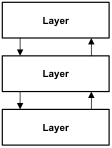
\includegraphics[scale=1, max size={\textwidth}{\textheight}]{M9-1}
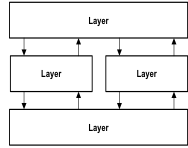
\includegraphics[scale=1, max size={\textwidth}{\textheight}]{M9-2}
\caption{Layered Architecture Different Implementations}
\label{M9}
\end{center}
\end{figure}
\item \textbf{Client – Server Architecture:} Distributed systems that are accessed over the Internet are normally organized as client–server systems. In a client–server system, the user interacts with a program running on their local computer (e.g., a web browser or phone-based application). This interacts with another program running on a remote computer (e.g., a web server). The remote computer provides services, such as access to web pages, which are available to external clients. This client–server model, is a very general architectural model of an application. It is not restricted to applications distributed across several machines. You can also use it as a logical interaction model where the client and the server run on the same computer.
In a client–server architecture, an application is modeled as a set of services that are provided by servers. Clients may access these services and present results to end users. Clients need to be aware of the servers that are available but do not know of the existence of other clients. Clients and servers are separate processes. The client-server style is the most frequently encountered of the architectural styles for network-based applications \cite{M17}. Client - Server components are: Client triggers process, Server reactive process \cite{M48}. Clients make requests that trigger reactions from servers, as presented in figure \ref{ClientServerInteraction} presented in page \pageref{ClientServerInteraction}. Variety of Client – Server systems are surveyed in \cite{M49,M50}. Client – Server architecture mainly consists of two layers: Single Server and many clients. Figure \ref{M10} presented in page \pageref{M10} depicts Client – Server Architecture different implementations. A Client-Server system is one in which the server performs some kind of service that is used by many clients \cite{M10}. The clients take the lead in the communication. The basic form of client-server does not constrain how application state is partitioned between client and server components, it is often referred to by the mechanisms used for the connector implementation, such as remote procedure call or message-oriented middleware \cite{M17}.
\begin{figure}
\begin{center}
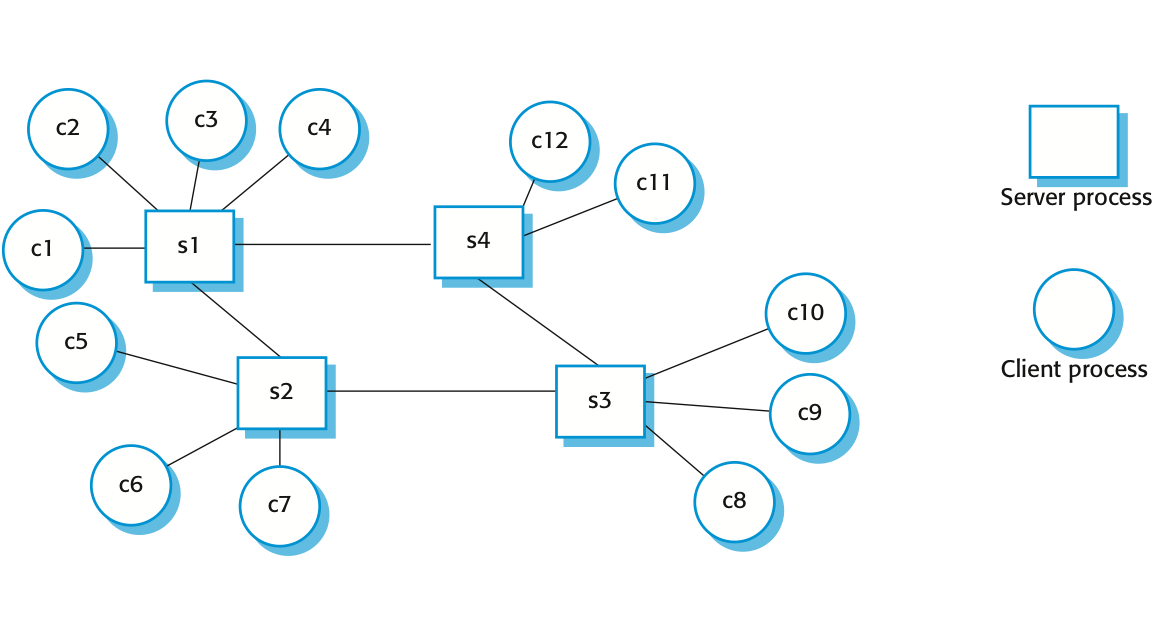
\includegraphics[scale=.8, max size={\textwidth}{\textheight}]{ClientServerInteraction}
\caption{Layered Architectural Model of Client-Server \cite{SWE9}}
\label{ClientServerInteraction}
\end{center}
\end{figure}

\begin{figure}
\begin{center}
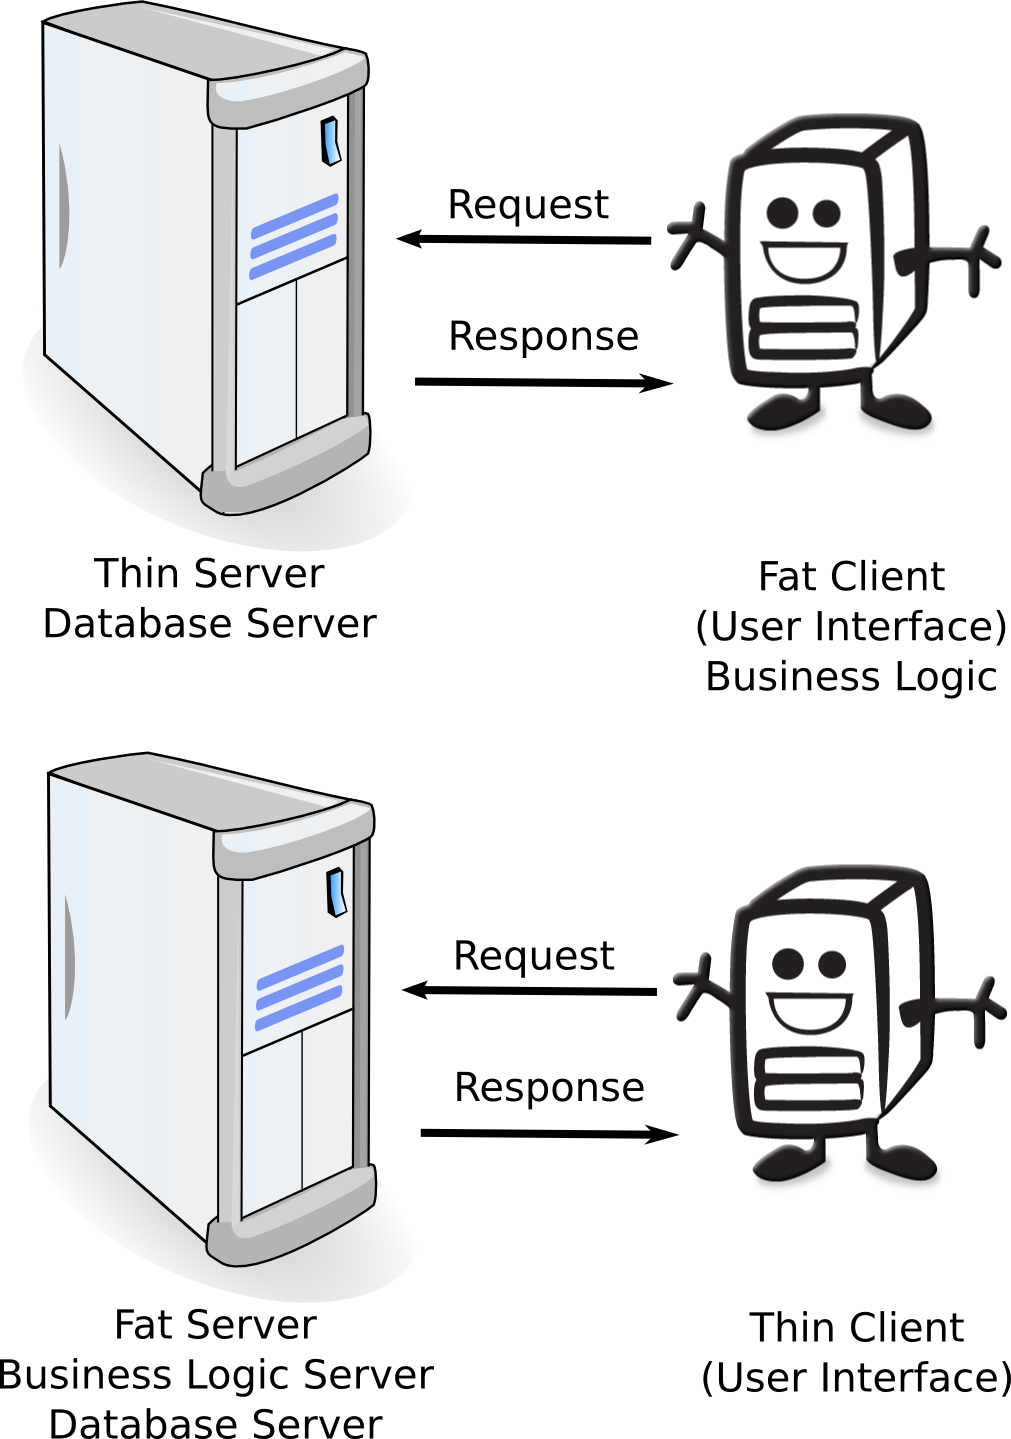
\includegraphics[scale=.5, max size={\textwidth}{\textheight}]{M10}
\caption{Client - Server Architecture Different Implementations}
\label{M10}
\end{center}
\end{figure}
\item \textbf{N-Tier Software Architecture:} N-Tier architecture is a Client-Server architecture combined with the Layered architecture where N equals three or higher \cite{M10}. Three-Tier architecture is an example of N-Tier architecture. Figure \ref{M11} presented in page \pageref{M11} depicts Three-Tier Architecture. Three-Tier architecture consists of three layers: Presentation, Application, and \gls{DB}.
\begin{figure}
\begin{center}
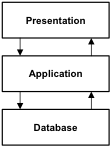
\includegraphics[scale=1.3, max size={\textwidth}{\textheight}]{M11}
\caption{Three Tier Architecture}
\label{M11}
\end{center}
\end{figure}
\begin{itemize}
\item \textbf{Presentation Layer}: deals with user interactions. Thin clients interface do not contain business logic, just code required to process user input, send requests to the server, and show the results of these requests.
\item \textbf{Application Layer}: processes client requests. It is the actual web application that performs all functionality specific to the web application. However, it does not store the persistent data itself. Whenever it needs data of any importance, it contacts the \gls{DB} server. 
\item \textbf{\gls{DB} Layer}: contains \gls{DB} and \gls{DBMS} (\gls{DBMS}).
\end{itemize}
\end{itemize}
Other applications can be divided into four layers \cite{SWE9}. Figure \ref{FouTier} presented in page \pageref{FouTier} shows that four Layers applications can be:
\begin{enumerate}
\item A presentation layer that is concerned with presenting information to the user and managing all user interaction;
\item A data management layer that manages the data that is passed to and from the client. This layer may implement checks on the data, generate web pages, etc.;
\item An application processing layer that is concerned with implementing the logic of the application and so providing the required functionality to end users;
\item A \gls{DB} layer that stores the data and provides transaction management services, etc.
\end{enumerate}
\begin{figure}
\begin{center}
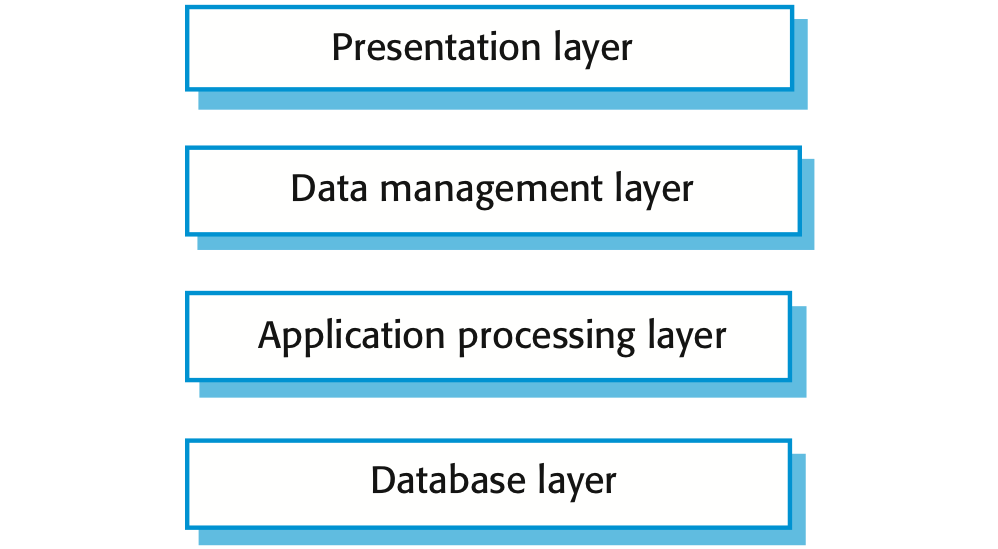
\includegraphics[scale=1.2, max size={\textwidth}{\textheight}]{FourTier}
\caption{Layered architectural model for client–server application \cite{SWE9}}
\label{FouTier}
\end{center}
\end{figure}

In the second and third tier there can be multiple instances, because of scalability, load-balancing and redundancy [10]. N-tier architecture (with N more than 3) is really 3 tier architectures in which the middle or bottom tier is split up into new tiers. Figures \ref{M12}, \ref{M13}, \ref{M14}, and \ref{M15} present different implementations of N-Tier architecture.
Figure \ref{M12} presented in page \pageref{M12} shows the simplest implementation of Three-Tier architecture, where the most left layer that includes Smart Phone, Cell Phone, and PC presents required logic to display information and validate user inputs. Business logic ‘presented in applications’ required to provide web applications to users are present on the Business Logic server. Required data to support those applications are present in the \gls{DB} server.
\begin{figure}
\begin{center}
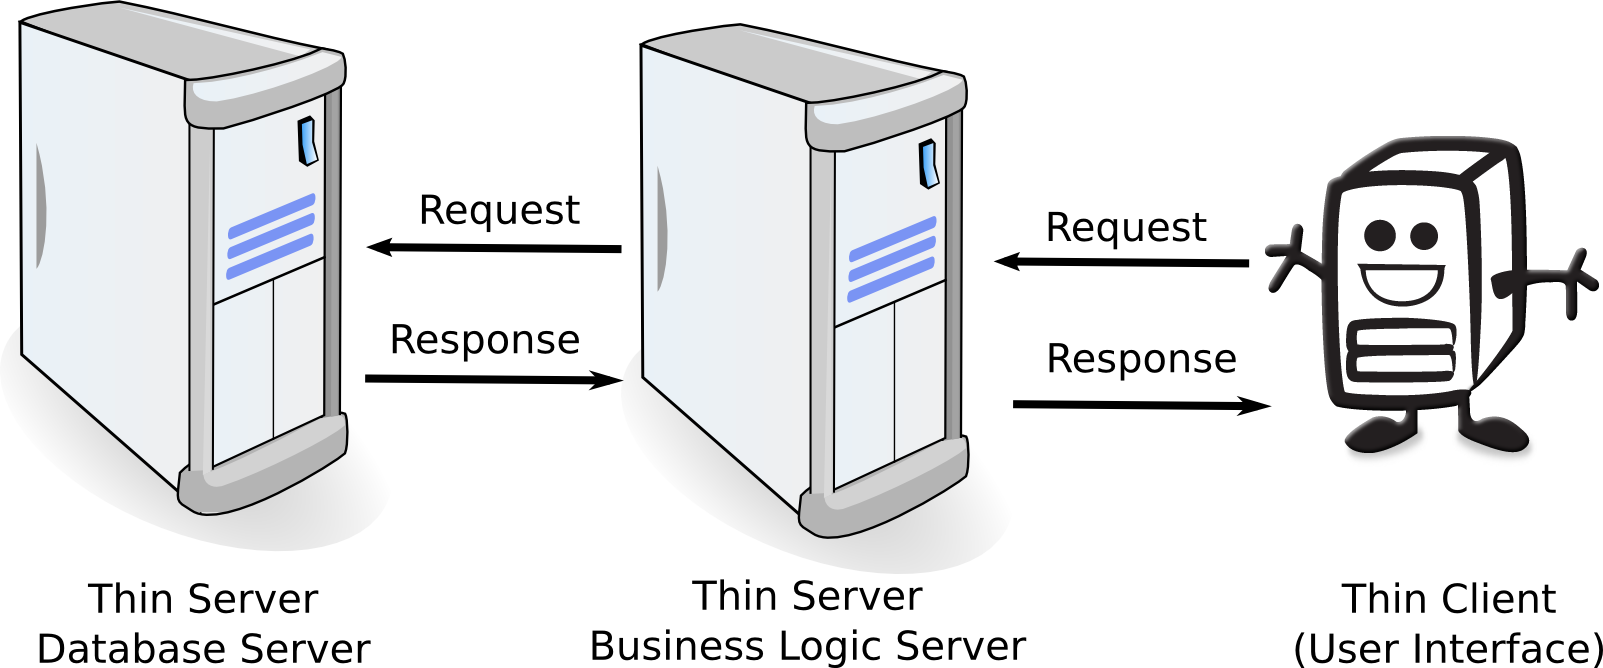
\includegraphics[scale=.3, max size={\textwidth}{\textheight}]{M12}
\caption{Three Tier Architecture Implementation}
\label{M12}
\end{center}
\end{figure}

Figure \ref{M13} presented in page \pageref{M13} illustrates the repetition of data layer by presenting more than one \gls{DB} server. \gls{DB} servers can be connected together or separated. Business logic server can connect to both \gls{DB} servers, or connect to one \gls{DB} server incase \gls{DB} servers are connected together. Servers’ connections is an architectural decision that software architect shall consider while designing software architecture.

\begin{figure}
\begin{center}
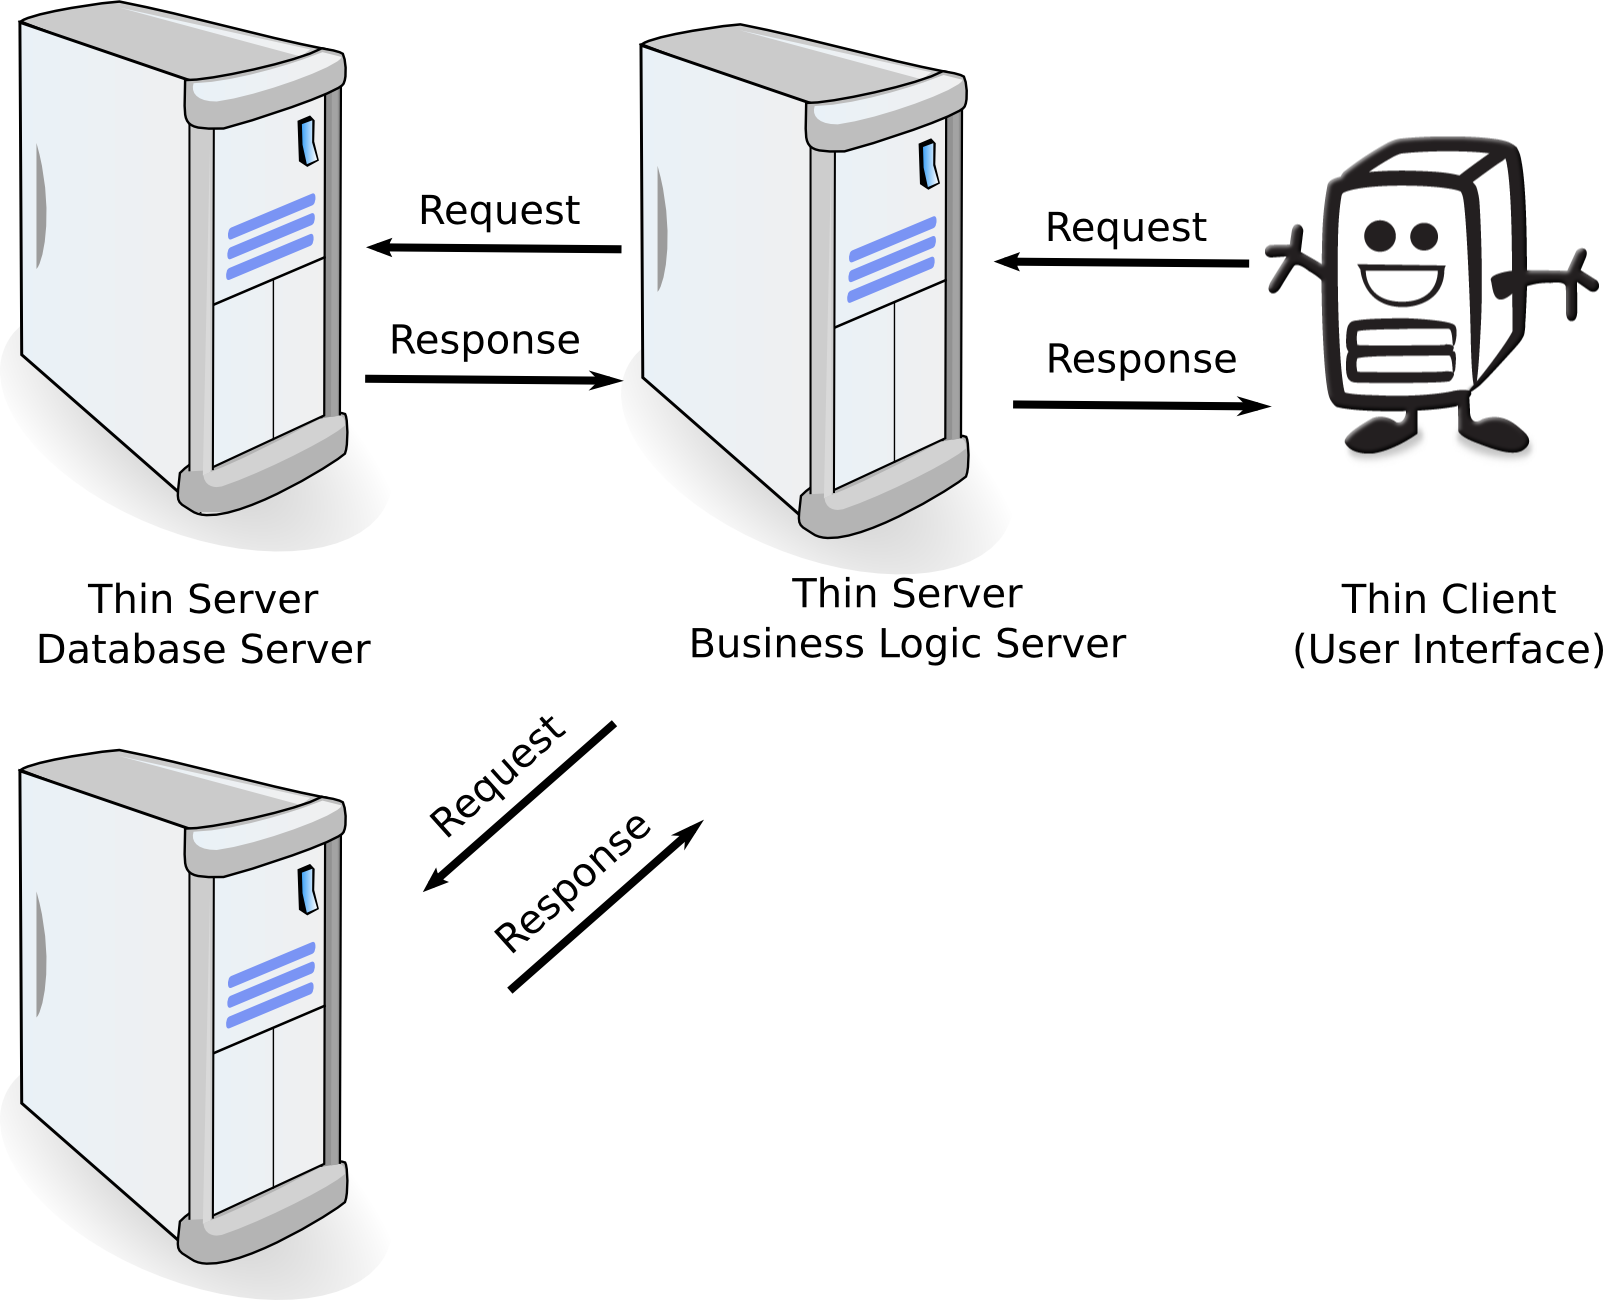
\includegraphics[scale=.3, max size={\textwidth}{\textheight}]{M13}
\caption{Three Tier Architecture First Implementation}
\label{M13}
\end{center}
\end{figure}

Figure \ref{M14} presented in page \pageref{M14} presents another N-Tier implementation which replicates business logic servers. Scalability can force such a solution. Business logic servers can be connected to each other or not based on application requirements.

\begin{figure}
\begin{center}
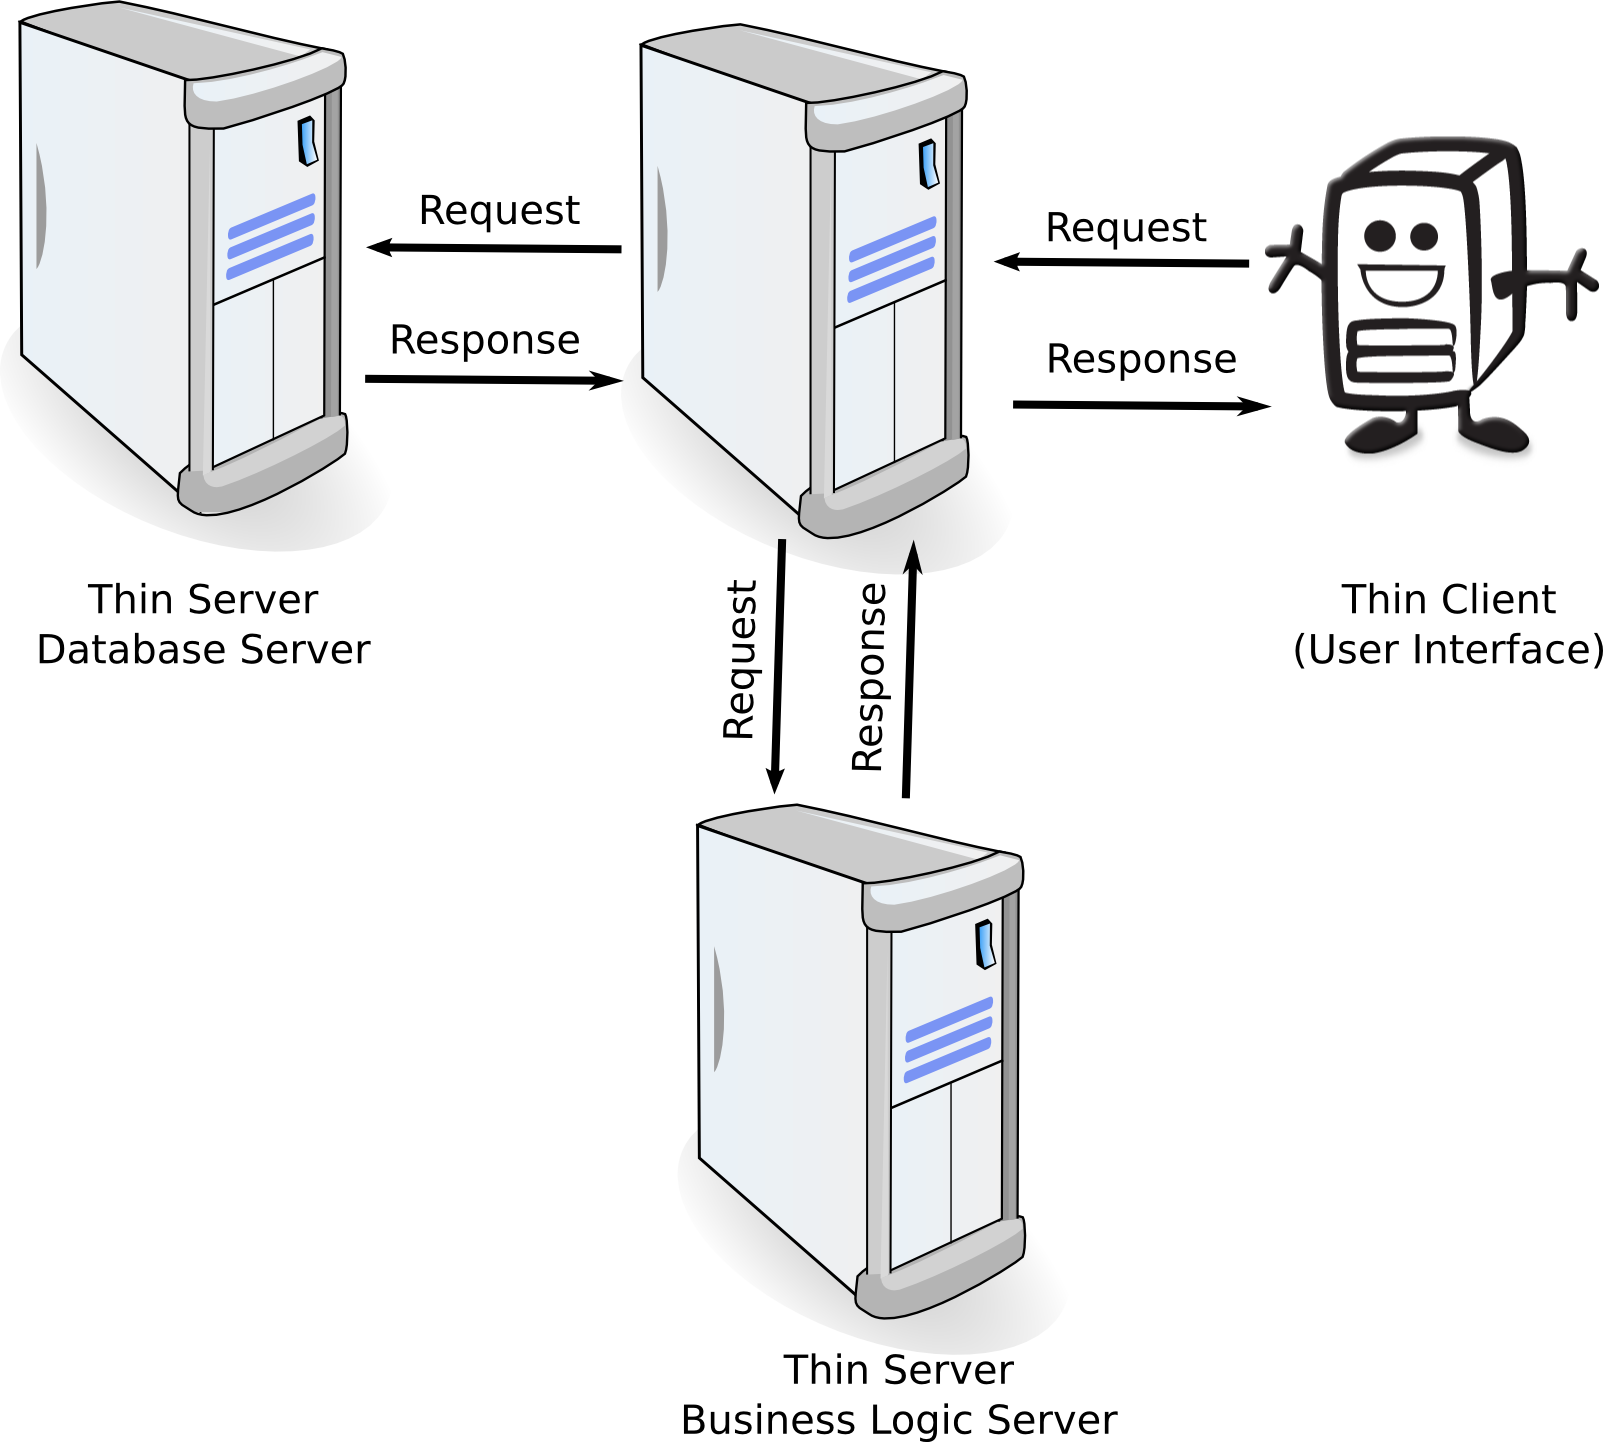
\includegraphics[scale=.3, max size={\textwidth}{\textheight}]{M14}
\caption{Three Tier Architecture Second Implementation}
\label{M14}
\end{center}
\end{figure}

Figure \ref{M15} presented in page \pageref{M15} presents the third N-Tier implementation where business logic and \gls{DB} servers are replicated. Large scaled institutions require this type of architectures to face increasing requirements. N-Tier Architecture serves integration by forcing enterprises to implement standard software at each tier. Even if different software is implemented, by connecting each tier to the other, enterprises overcome integration problems. N-Tier has been widely accepted in today's organizations as the standard architecture. Unfortunately, N-Tier architecture does not define what tier should include, how tiers should connect to each other, thus, architectural decisions still needs to be taken by software architect. Table \ref{MT4} shows driving and restraining forces on adopting wide standard software as an integration solution \cite{M25, M26, M27}. Unfortunately, this integration technique is not well suited for process level integration. Figure \ref{EnterpriseSoftware} presented in page \pageref{EnterpriseSoftware} presents another view of enterprise software pitfalls.

\begin{figure}
\begin{center}
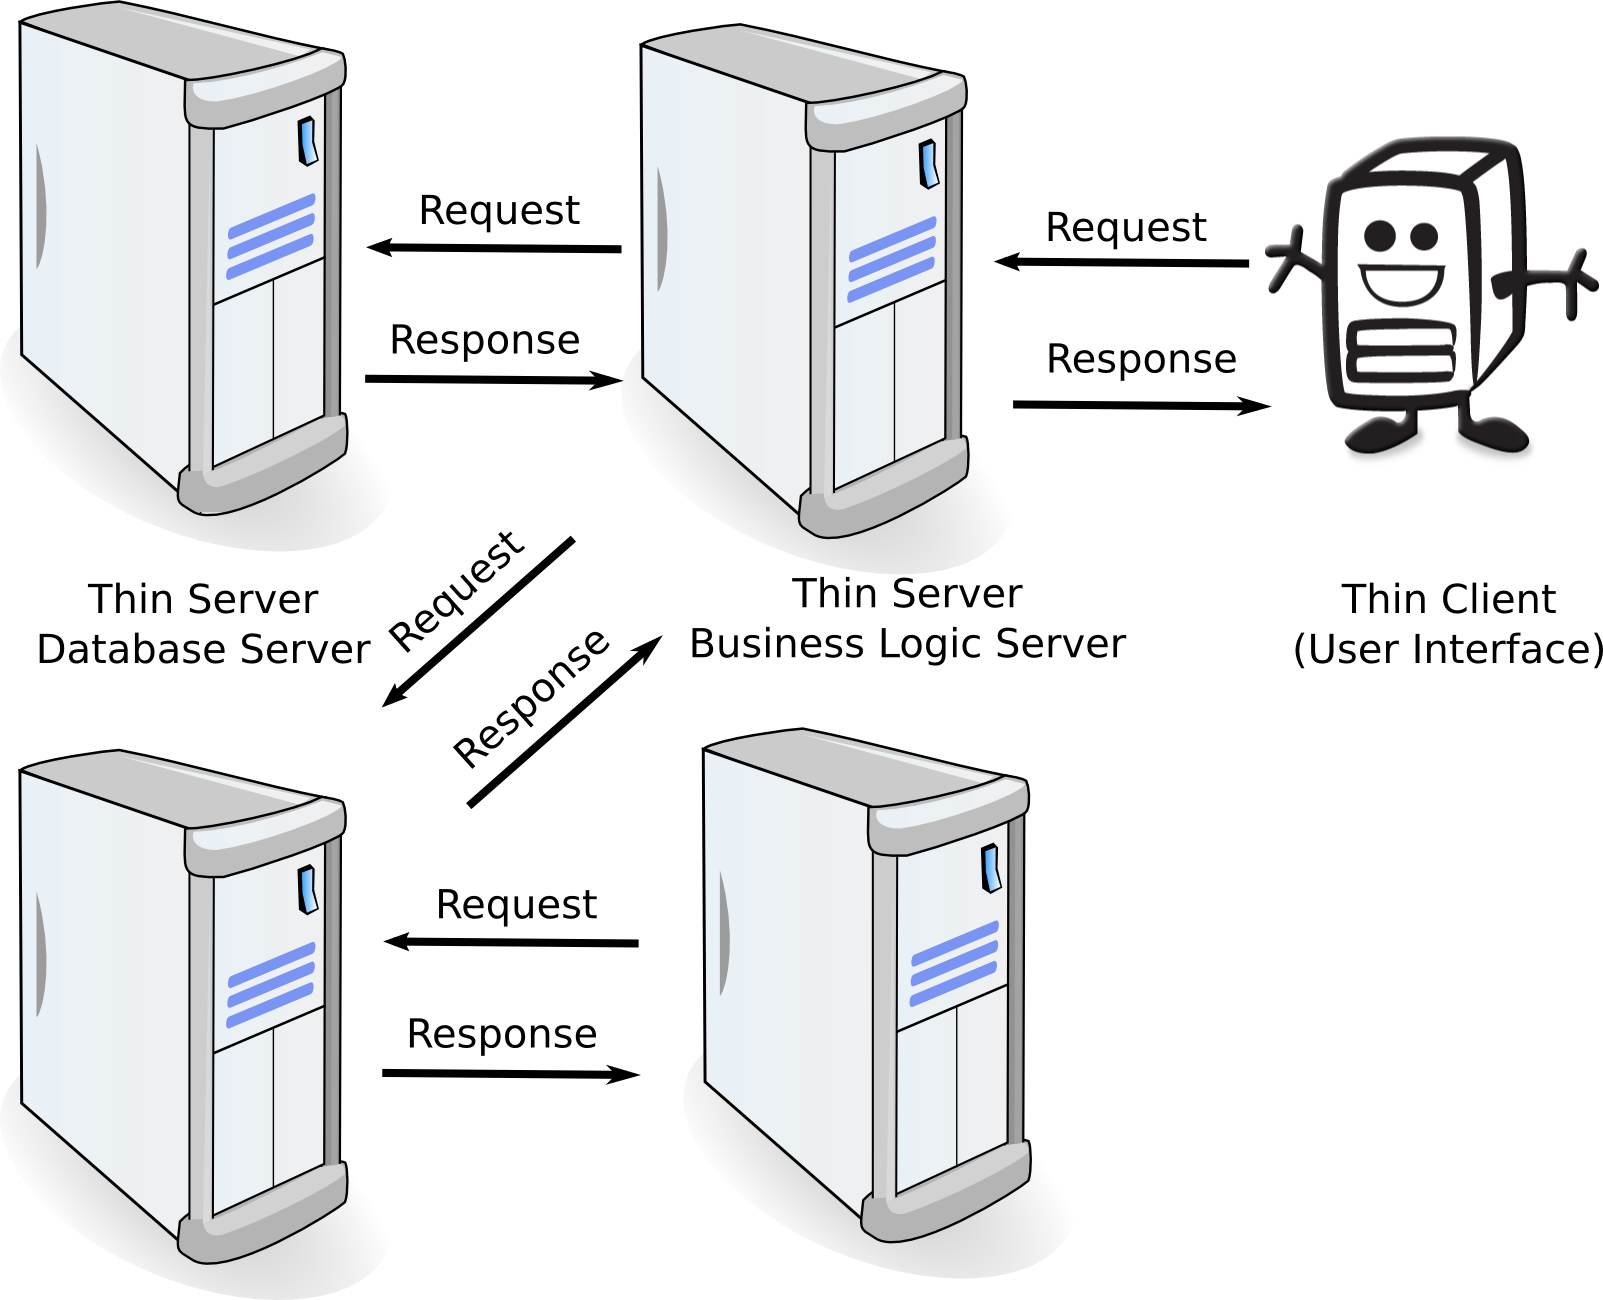
\includegraphics[scale=.3, max size={\textwidth}{\textheight}]{M15}
\caption{Three Tier Architecture Third Implementation}
\label{M15}
\end{center}
\end{figure}

\begin{table}
\begin{center}
\caption{Adopting Standard Enterprise Software Pitfalls}
\begin{tabularx}{\textwidth}{|X|X|}
\hline Driving Forces & Restraining Forces \\
\hline Easier access to enterprise wide data & Mergers and acquisitions \\
\hline Reduced development time & Departments have different needs\\
\hline Reduced maintenance costs & Dependence on different software\\
\hline & Conversion to new software\\
\hline
\end{tabularx}
\end{center}
\label{MT4}
\end{table}

\begin{figure}
\begin{center}
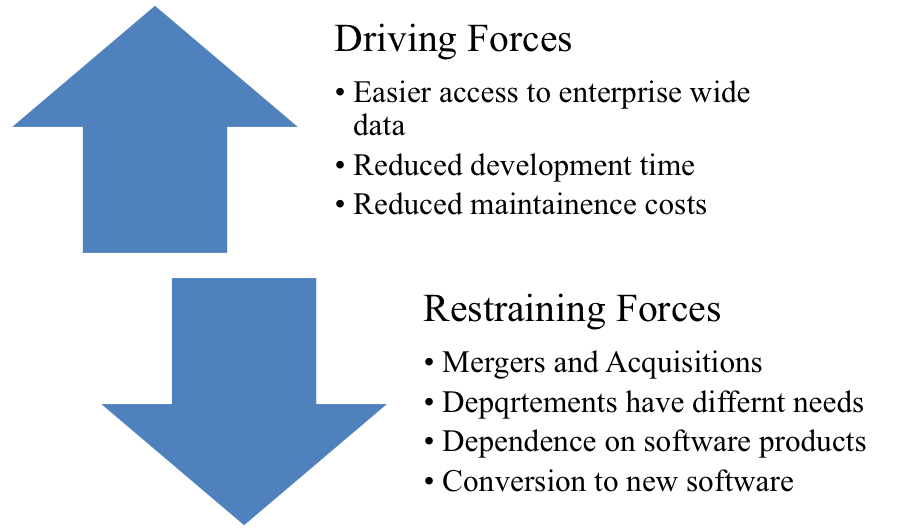
\includegraphics[scale=1, max size={\textwidth}{\textheight}]{EnterpriseSoftware}
\caption{Adopting Standard Enterprise Software Pitfalls}
\label{EnterpriseSoftware}
\end{center}
\end{figure}

\subsubsection{Middleware Integration Technique}
Middleware integration facilitates communication between applications in order to exchange data and business logic. This communication is either: Point-To-Point, or Multi-Applications.
\begin{itemize}
\item \textbf{Point To Point Middleware:} Point To Point refers to direct connection and communication between two applications. This direct communication can be presented by two methods: Adapters, and Remote Procedure Calls (\gls{RPC}s).
\begin{itemize}
\item Application Adapters: In this case, a special purpose adapter is presented to integrate two applications and provide communication and exchange of data among them. Examples of adapters are presented in [51]. This adapter is capable of transforming data syntax and semantics, and managing communication among connected application. Special adapters are presented for each application.
\item \gls{RPC}: an \gls{RPC} allows execution of program logic on a remote system by calling local routine. This calling is done via special message between client and server \footnote{In this case, machine that initiated \gls{RPC} is considered Client, while the machine that holds code to be invoked and executed by reception of \gls{RPC} is Server.}.
\end{itemize}
\item \textbf{Multi-Applications Middleware}: The components in a distributed system may be implemented in different programming languages and may execute on completely different types of processor. Models of data, information representation, and protocols for communication may all be different. A distributed system therefore requires software that can manage these diverse parts, and ensure that they can communicate and exchange data.
The term ‘middleware’ is used to refer to this software—it sits in the middle between the distributed components of the system. Middleware is normally implemented as a set of libraries, which are installed on each distributed computer, plus a run-time system to manage communications. Middleware is general-purpose software that is usually bought off the shelf rather than written specially by application developers. Examples of middleware include software for managing communications with databases, transaction managers, data converters, and communication controllers. Multi-Applications middleware relies heavily on messages in order to hide complexity of communication between systems. It is not acceptable to provide adapters for the whole system; instead, a middleware is required to integrate applications within the system \cite{M36}. Exchanging messages enabled integration on software level. Table \ref{MT5} presented in page \pageref{MT5} depicts driving and restraining forces of adopting message routing integration technique. Software architectures supported different implementations for integrating applications via exchanging messages. Those architectures include: Message Broker, Message Bus, and Broker. Figure \ref{MessageRouting} presented in page \pageref{MessageRouting} depicts another view of adopting message routing pitfalls.
\begin{table}
\begin{center}
\caption{Adopting Message Routing Pitfalls}
\begin{tabularx}{\textwidth}{|X|X|}
\hline Driving Forces & Restraining Forces \\
\hline Consistent enterprise wide data & Costs of development \\
\hline Reduced development time & Different semantics in data sources\\
\hline Reduced maintenance costs & Semantic translation\\
\hline Minimal effect on systems & Lack of industry standard definitions\\
\hline & Deciding what data to route \\
\hline & Delays getting data updates distributed \\
\hline & Data quality issues\\
\hline & Brittleness of fixed record exchange \\
\hline
\end{tabularx}
\end{center}
\label{MT5}
\end{table}

\begin{figure}
\begin{center}
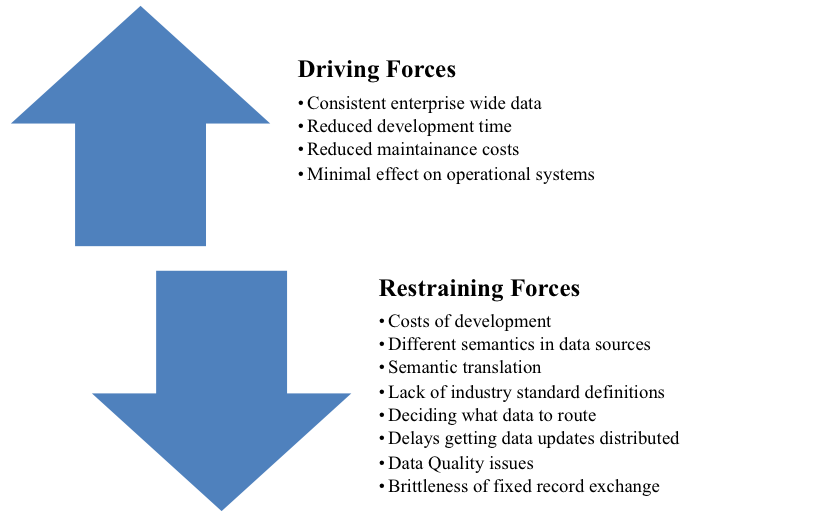
\includegraphics[scale=1.6, max size={\textwidth}{\textheight}]{MessageRouting}
\caption{Adopting Message Routing Pitfalls}
\label{MessageRouting}
\end{center}
\end{figure}



\begin{itemize}
\item Message Bus: Message bus architecture connects all applications through the logical component known as Message Bus [28]. Message bus is responsible for delivering messages to destined applications. Sending application has no responsibility of direct connection with destined application. Sending application needs to prepare the message in the message bus agreed format, and delivers it to the message bus. Figure \ref{M16} presented in page \pageref{M16} depicts how message bus architecture works. There are three options for subscribing the application to the Message Bus \cite{M52}:
\begin{itemize}
\item List-Based Publish/Subscribe: There are managed lists for subscribers. All subscribers receive certain messages when they are sent to the bus.
\item Broadcast-Based Publish/Subscribe: Messages are sent to the all connected applications.
\item Content-Based Publish/Subscribe: it enables Message Bus to investigate message contents to determine recipient of the message.
\end{itemize}
Limitations include that message bus can expose only one interface. In order for an application to be part of the architecture, it should implement the message bus interface, use the message bus messages type, and registers itself to the message bus. Performance issues are also a potential problem; poor application partitioning can create excessively high volumes of messages, and some use cases can be impacted through high network latency \cite{M53}. One of middleware integration techniques implementation that utilizes message bus is \gls{CORBA}. \gls{CORBA}: is the acronym for Common Object Request Broker Architecture, OMG's open, vendor-independent architecture and infrastructure that computer applications use to work together over networks \cite{M54}. \gls{CORBA} applications are composed of objects. \gls{CORBA} creates a distributed objects infrastructure which makes activating and accessing remote objects transparent \cite{M55}. Legacy application is wrapped in code with \gls{CORBA} interfaces and opened up to clients on the network. Systems wrapped with \gls{CORBA} can be integrated under \gls{CORBA} architecture. Table \ref{MT6} presented in page \pageref{MT6} depicts driving and restraining forces of adopting \gls{CORBA} as an integration technique implementation. Figure \ref{MessageRouting} presented in page  Figure \ref{CORBA} presented in page \pageref{CORBA} depicts another view of adopting message CORBA pitfalls.
\begin{figure}
\begin{center}
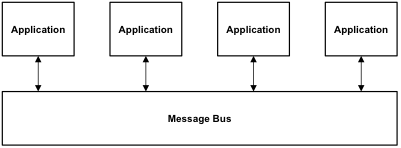
\includegraphics[scale=1, max size={\textwidth}{\textheight}]{M16}
\caption{Message Bus Architecture}
\label{M16}
\end{center}
\end{figure}

\begin{table}
\begin{center}
\caption{Adopting Message CORBA Pitfalls}
\begin{tabularx}{\textwidth}{|X|X|}
\hline Driving Forces & Restraining Forces \\
\hline Interoperable networked applications & Different semantics in data sources \\
\hline Reduced development time & Semantic translations\\
\hline Reduced maintenance costs & Lack of industry standard definitions\\
\hline & Lack of CORBA/DCOM product support \\
\hline & Perceived CORBA/DCOM complexity \\
\hline & Effect on operational systems of data requests\\
\hline & Merges and acquisitions\\
\hline
\end{tabularx}
\end{center}
\label{MT6}
\end{table}

\begin{figure}
\begin{center}
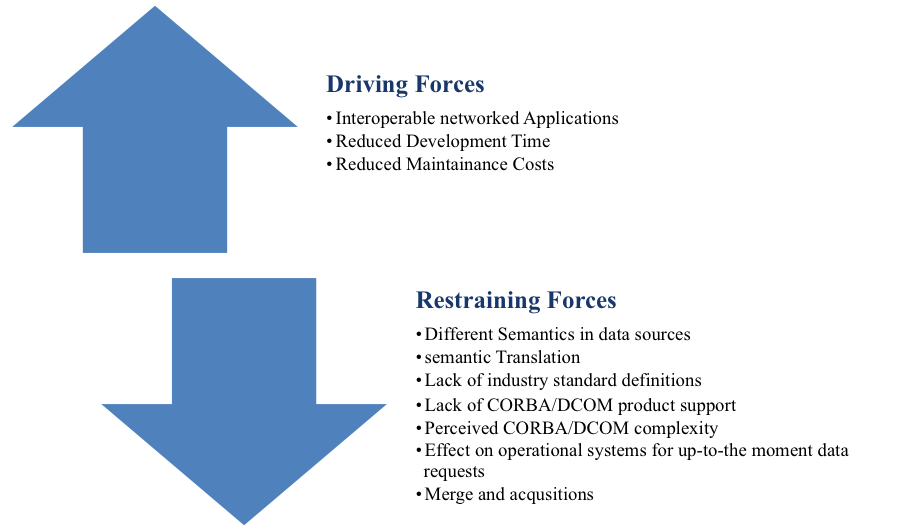
\includegraphics[scale=1, max size={\textwidth}{\textheight}]{CORBA}
\caption{Adopting Message CORBA Pitfalls}
\label{CORBA}
\end{center}
\end{figure}


\item Message Broker: The message broker can expose different interfaces to the collaborating applications, and it can translate messages between these interfaces \cite{M26}. Message broker does not enforce a common interface on the applications, thus handles shortages of Message Bus. Figure \ref{M17} presented in page \pageref{M17} depicts Message Broker architecture. Subscribing options are the same as mentioned in Message Bus architecture. Commercially, Message Broker is referred to as Message Oriented Middleware (MOM). One commercial implementation of MOM is Microsoft BizTalk Server \cite{M56}. Software Architectures that support Message Broker includes: Broker ‘\gls{SOA}’.\index{Service Oriented Architecture}
\item \gls{SOA}: Servers can register and deregister with the broker. If a server fails, it will be automatically (after a timeout) unregistered by the broker. Broker handles user requests by providing user capability to find different service providers, pick the most suitable one, and utilizes its service \cite{M10}. The client requests a specific service. It formats its request in a specific format and sends it to its broker. The broker then selects the most suitable server to process the request. When the link between the client and the server is set up, they may start communicating directly, freeing the broker. Figure \ref{M18} presented in page \pageref{M18} depicts broker architecture mechanism of action. \gls{CORBA} was attempted to satisfy Broker architecture requirements, unfortunately \gls{CORBA} itself has shortages that inhibited it from being the standard integration solution. \gls{SOA} is the most suitable architecture to integrate organizations on process level. \gls{SOA} integration is the strongest integration provided to organizations \cite{M33}. With this importance for \gls{SOA}, \gls{CORBA} limitations were addressed among software vendors and industry standards creators. Web services were presented as the industry solution to overcome \gls{CORBA} limitations. Table \ref{MT7} presented in page \pageref{MT7} depicts driving and restraining forces of adopting Web services as an integration solution. Figure \ref{Webservices} presented in page \pageref{Webservices} depicts another view of adopting Web services pitfalls. With those driving forces mentioned for adopting Web services, and with the fact that \gls{SOA} being the only software architecture capable on providing a process level integration, combining both Web services and \gls{SOA} is almost a must. Most software capabilities will be provided and consumed as services. When the service is abstracted from the implementation it is possible to consider various alternative options for delivery and collaboration models [96]. 
\end{itemize}
\end{itemize}
\index{Service Oriented Architecture}
\begin{figure}
\begin{center}
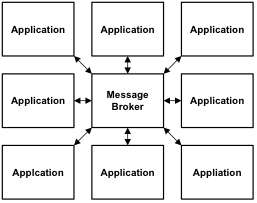
\includegraphics[scale=1, max size={\textwidth}{\textheight}]{M17}
\caption{Message Broker Architecture}
\label{M17}
\end{center}
\end{figure}

\begin{figure}
\begin{center}
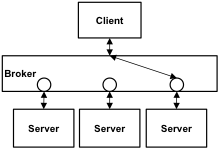
\includegraphics[scale=1, max size={\textwidth}{\textheight}]{M18}
\caption{Broker Architecture}
\label{M18}
\end{center}
\end{figure}

\begin{table}
\begin{center}
\caption{Adopting Web services Pitfalls}
\begin{tabularx}{\textwidth}{|X|X|}
\hline Driving Forces & Restraining Forces \\
\hline Interoperable networked applications & Different semantics in data sources \\
\hline Emerging industry wide standards & Effect on operational systems and data requests\\
\hline Support of Web services in products & \\
\hline Easier exchange of data & \\
\hline Reduced brittleness using tags & \\
\hline Reduced development time & \\
\hline Availability of external services & \\
\hline Availability of training and tools & \\
\hline Mergers and acquisitions & \\
\hline Semantic translation & \\
\hline
\end{tabularx}
\end{center}
\label{MT7}
\end{table}

\begin{figure}
\begin{center}
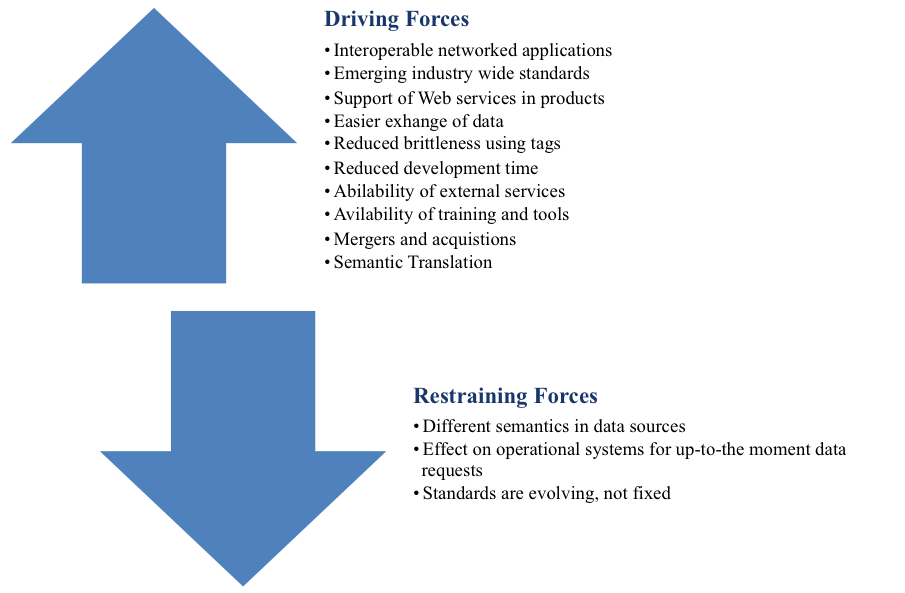
\includegraphics[scale=1, max size={\textwidth}{\textheight}]{Webservices}
\caption{Adopting Web services Pitfalls}
\label{Webservices}
\end{center}
\end{figure}


\begin{figure}
\begin{center}
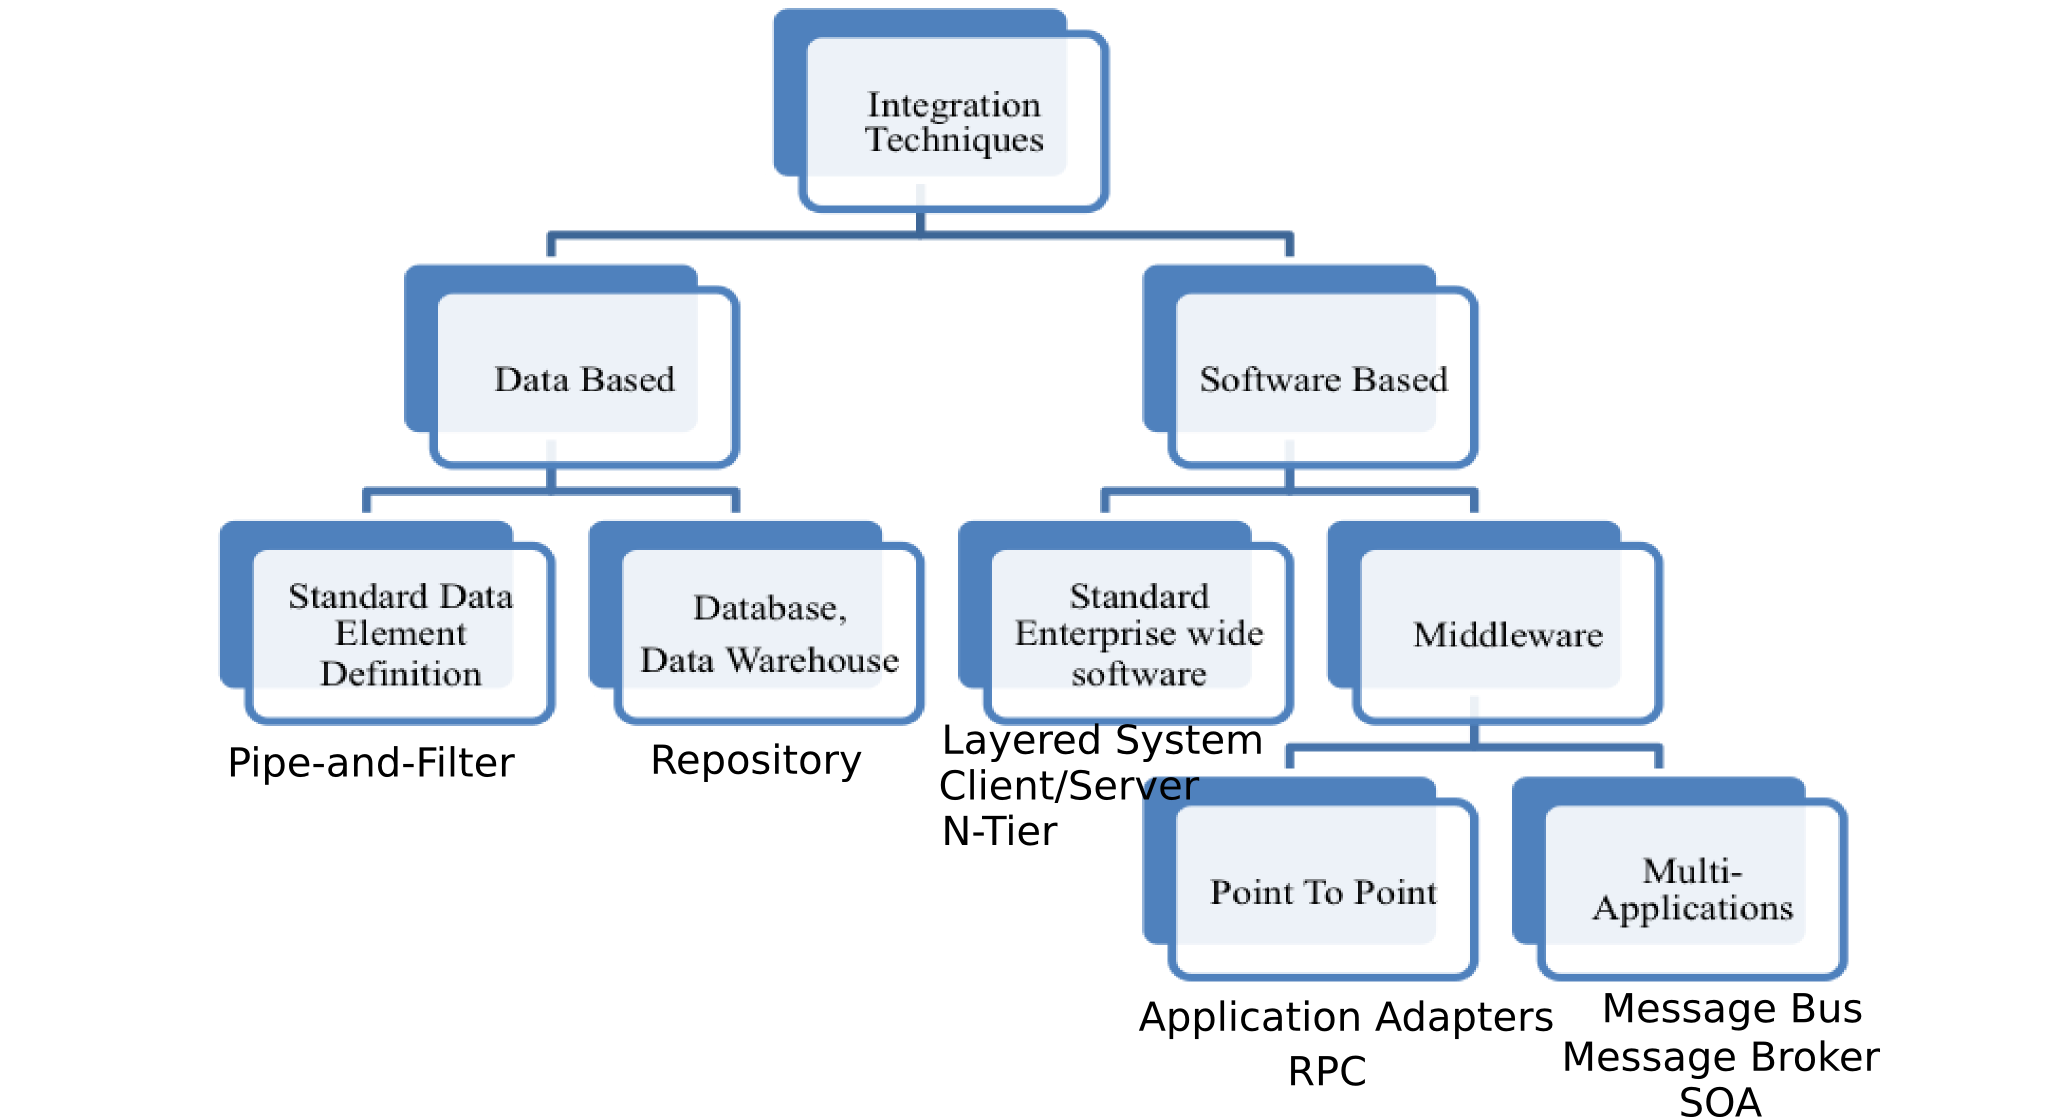
\includegraphics[scale=.35, angle=90, max size={\textwidth}{\textheight}]{M19}
\caption{Integration Techniques and Software Architectures}
\label{M19}
\end{center}
\end{figure}

\section{SOA Selected Topics}
\subsection{Relationship Between EA and SOA}
\index{Service Oriented Architecture}
\gls{SOA} can be applied to different levels of scope: from the enterprise level to individual project level. \gls{SOA} is integral to successful \gls{EA}, and for some organizations it renews the value of EA. A service portfolio is one of the primary linkages of \gls{SOA} to EA as enterprise architects play a major role in advancing the use and awareness across the enterprise of the service portfolio. The service portfolio is an enterprise asset, and enterprise architects must play a governance role in the use of services, vertically and horizontally in the enterprise. An architectural review board that includes enterprise architects will govern the service portfolio as an enterprise asset. EA is an architectural discipline that merges strategic business and IT objectives with opportunities for change and governs the resulting change initiatives. \gls{SOA} represents a strategic business and IT objective that EA helps govern across multiple project instances. EA uses \gls{SOA} principles and assets (e.g., service portfolio and \gls{SOA} reference models) to integrate with business architecture, information architecture, application architectures, and infrastructure architectures. EA has an enterprise-wide focus and addresses both \gls{SOA} and non-\gls{SOA} aspects of the enterprise.\index{Enterprise Architecture}\index{Service Oriented Architecture}
\subsection{Services Identification Methods}
Services are optimally identified using three complementary techniques that provide a balance between tactical imperatives and strategic vision:
\begin{itemize}
\item Goal service modeling looks at business opportunities, strategy, and business goals to both confirm and validate that candidate services have been identified, which fulfill goals and enable the business strategy.
\item Domain decomposition focuses on business process modeling, rules, information, and potential variability of services.
\item Asset analysis addresses the reality that businesses have accumulated legacy systems and applications that must be integrated, enhanced, or leveraged. This bottom-up approach looks at the existing application portfolio and other assets that can be used in identifying candidates for service exposure. In contrast, goal service modeling combines the top-down (domain decomposition) and bottom-up (asset analysis) approaches and pulls them together into alignment.
\end{itemize}

\subsection{CBA}
\gls{CBA} is a software architecture that is based on components. A component is a software object, meant to interact with other components, encapsulating certain functionality or a set of functionality. A component has a clearly defined interface and conforms to a prescribed behavior common to all components within an architecture \cite{SOAvsCBA}. A component model is probably used for the developing and executing of components. This model defines a framework, which defines structural requirements for connection- and composition options as well as behavior-oriented requirements for collaboration options to the components. Beyond that a component model provides an infrastructure which implements frequently used mechanism like persistence, message-exchange, security  and versioning. The idea is to build exchangeable software units through  clearly defined interfaces. Different manufactures offer platforms like DCOM, JavaBeans, Enterprise JavaBeans, and CORBA. 
There is no clear dividing line between \gls{SOA} and Component Based Architecture. In principle \gls{SOA} is the enhancement of Components: The individual services are single components, which can be linked to gain new business logic, new services or a new component. The big difference is the connection between and the possibilities of offering single services for third parties. For example, EJBs (especially Session Beans) can be designed to offer its business methods like services in a context free way. These services of this EJB can be used by other EJBs or clients. In a big company (or a coalition of parties gaining access to each others EJB’s) single departments could offer their services (in the shape of the business methods of the EJBs) for other departments, so that the same effect could be achieved as with services supporting \gls{SOAP}: The business methods of the EJBs 
represent the activities one department offers. Other departments could use these services for their belongings and perhaps use them in a way the business method wasn't built for. So, this usage of Enterprise JavaBeans could be seen as service oriented too. \index{Service Oriented Architecture}

\subsection{Agile/OOAD and SOA}
Many of the current system development methods focus on making IT more effective, cheaper, or faster, whereas \gls{SOA} methods focus on making the business and IT more effective and faster. \gls{SOA} methods provide prescriptive software engineering guidance by addressing the following:\index{Service Oriented Architecture}
\begin{itemize}
\item They provide guidance on how to identify and develop reusable business services that can be reconfigured to provide new business capability or repurposed to serve different business processes or market opportunities.
\item They focus on how to reduce, using services, the lifetime cost of the application.
\item They reduce system development activities, allowing for an accelerated system development process using services.
\item They allow engineer applications to be built for change.
\end{itemize}
To identify and build reusable, reconfigurable, and flexible services as business assets, you must change existing methods to accommodate the identification, specification, and realization of five primary constructs:
\begin{itemize}
\item Business processes 
\item Services
\item Components
\item Information
\item Rules/policies (and their flows)
\end{itemize}
A business service catalog will be the result, which will grow over time, project by project. Business services should be reused across applications and channels supporting vertical and horizontal business processes. \gls{SOA} methods provide guidance on how to identify, specify, and realize reusable business services.\index{Service Oriented Architecture}

\section{Summary}
\gls{EA} is the framework of business, IT, information, and software architectures. Software architecture design is an important step within system design because software architectures should satisfy non-functional as it satisfies functional system requirements. Non-functional requirements like integration, interoperability, and agility can be satisfied by architectural design, if considered. Software architecture satisfaction to integration; as one of the non-functional requirements, is used in this chapter as an indicator to the software architecture of non-functional requirements satisfaction. 
The most common Software architectures are mapped to presented integration techniques; highlighting architectures driving and restraining forces, and its satisfaction level to system non-functional requirements. Figure \ref{M19} presented in page \pageref{M19} summarizes the integration techniques and different software architectures presented as an enabler of each technique. Each one of the presented software architecture has its driving and restraining forces which presents strengths and weaknesses of each one. Web services based \gls{SOA} achieved the maximum driving forces and satisfied almost all non-functional requirements addressed in the comparative study.\index{Enterprise Architecture}\index{Service Oriented Architecture}

\section{Review Questions}
\begin{enumerate}
\item What are Enterprise Architecture Dimensions?
\item Discuss the importance of \gls{SW} Architecture.
\item What are the advantages of Distributed \gls{SW} Approaches?
\item List, and describe in brief the most common \gls{SW} architecture patterns.
\item What are the main SW architectures integration techniques?
\item What are the advantages and disadvantages of each of the following techniques in \gls{SW} integration:
\begin{enumerate}
\item Standard Data Element Definition
\item Middleware Integration Technique
\item Standard Enterprise Wide Software
\item Middleware
\end{enumerate}
\item What is the relationship between \gls{EA} and \gls{SOA}?
\item What is CBA?
\end{enumerate}

\section{Exercises and Labs}
In Labs, you shall be getting familiar with Java programming language, as it is the programming language we will be using to build, deploy, and consume different online Webservices and \gls{SOA} systems presented in this book.

\chapter{Service Oriented Architecture}
\label{SOA}
\section{Introduction}
A web service is an instance of a more general notion of a service, which is defined as:
“an act or performance offered by one party to another. Although the process may be tied to a physical product, the performance is essentially intangible and does not normally result in ownership of any of the factors of production”.
The essence of a service, therefore, is that the provision of the service is independent of the application using the service. Service providers can develop specialized services and offer these to a range of service users from different organizations.
\gls{SOA} are a way of developing distributed systems where the system components are stand-alone services, executing on geographically distributed computers. Standard \gls{XML}-based protocols, such as \gls{SOAP} and \gls{WSDL}, have been designed to support service communication and information exchange. Consequently, services are platform and implementation-language independent. Software systems can be constructed by composing local services and external services from different providers, with seamless interaction between the services in the system.
This chapter presents different topics related to \gls{SOA}, including: \gls{SOA} advantages, technologies, different methods of implementation, examples of \gls{IS} based on \gls{SOA}, and concludes with an important concept, that is \gls{ESB}.\index{Service Oriented Architecture}

\section{SOA}
\gls{SOA} is defined as the policies, practices, frameworks that enable application functionality to be provided and consumed as sets of services published at a granularity relevant to the service consumer. Services can be invoked, published and discovered, and are abstracted away from the implementation using a single, standards based form of interface [98 - 101]. \index{Service Oriented Architecture}
\subsection{SOA Advantages}\index{Service Oriented Architecture}
\gls{SOA} advantages are categorized into implementation, and organizational benefits. 
\subsubsection{Implementation Benefits}
Implementation benefits satisfy the loose coupling objective. Using a resource only via its published service and not by directly addressing the implementation gives system capabilities of [102]:
\begin{itemize}
\item Changes to the implementation by the service provider should not affect the service consumer. Services are exposed via standard interfaces and are thought about as black boxes that changes within it do not affect consumers.
\item Service consumer could choose an alternative instance of the same service type without modifying requesting application. As long as new service implements the same interface, theoretically there are no problems.
\item Service consumer and service provider do not have to implement same technologies for implementation, interface, or integration when Web services are used.
\end{itemize}
\subsubsection{Organizational / Business Benefits}
Businesses are dealing with two fundamental concerns: the ability to change quickly (agility), and the need to reduce costs [103]. Business must adapt quickly to internal factors such as acquisitions and restructuring, or external factors like competitive forces and customer requirements to remain competitive. Cost-effective, flexible IT infrastructure is needed to support the business. \gls{SOA} can realize several benefits to help organizations succeed. Organizational/Business benefits of adopting \gls{SOA} are:\index{Service Oriented Architecture}
\begin{itemize}
\item Leverage existing assets: by wrapping existing software applications as services instead or rebuilding new solutions from scratch.
\item Easier to integrate: integration on service level in order to satisfy business processes integration presents the highest integration technique that solved many problems as depicted in chapter three.
\item More responsive and faster time-to-adapt (Agility): the ability to compose new services out of existing ones provides a distinct advantage to an organization that has to be agile to respond to demanding business needs. Leveraging existing components and services reduces the time needed to go through the software development life cycle leading to rapid development of new business services and allows an organization to respond quickly to changes. \gls{SOA} provides the flexibility and responsiveness that is critical to businesses agility.
\item Reduce cost and increase reuse: with core business service exposed in a loosely coupled manner, they can be more easily used and combined based on business needs. This means less duplication of resources, more potential for reuse, and lower costs.\index{Service Oriented Architecture}
\end{itemize}
\section{SOA Technologies}
\index{Service Oriented Architecture}
\gls{SOA} implementations include: Software Agents, and Web services.
\subsection{Software Agents}
Software Agent is a computer system that is situated in some environment and is capable of autonomous actions in this environment in order to meet its design objectives [104,105]. 
Different \gls{SOA} implementations using different software agents are presented in [106 – 110]. \gls{SOA} implementation via mobile agents technology can be found in [108]. The main idea is about having one or more software agents perform certain task(s), those tasks can be exposed as services that compose \gls{SOA}.
Software agents have many classification criteria. Agents can be classified as either Desktop, Internet, or Intranet agents according to their action environment [111]. Many internet related agents can be classified into subcategories as presented in [112]. \gls{IA}s can be classified into Simple reflex agents, Model-based reflex agents, Goal-based agents, and Utility-based agents [113]. Agents can be also classified by application types, and by characteristics [114]. \index{Service Oriented Architecture}
Software Agents have characteristics that make them suitable to perform complex functionality. Characteristics include: Autonomy, Interactivity, Reactivity, Proactivity, Intelligence, and Mobility [114]. Agent is autonomous; it is capable of acting on its own. An agent is goal oriented, collaborative, and flexible, so, it must be autonomous. Agents are designed to interact with other agents, humans, or software programs (Interactivity). Instead of making a single agent conduct several tasks, additional agents can be created to handle un-delegated task. Agents perceive environment via preceptors [113] and respond to changes (Reactivity). Agents do not just act in response to their environment, but agents are able to exhibit goal-directed behavior by taking an initiative (proactive). Agent may need mobility to work on different machines. An agent with this capability is called mobile agent, it can transport itself across different system architectures and platforms, and is far more flexible than those that cannot. Many electronic commerce agents are mobile [114]. Mobile agent is an executing program that can migrate during execution from machine to machine in a heterogeneous network [110].
\subsubsection{Multi-Agent System}
Multi-Agent Systems (MASs) are becoming increasingly important: as a scientific discipline, as a software engineering paradigm, and as a commercially viable and innovative technology [115].
A Multi Agent is any system that contains [116]:
\begin{itemize}
\item Two or more agents;
\item At least one autonomous agent; and
\item At least one relationship between two agents where one satisfies goal of the other.
\end{itemize}
Many Multi-Agent frameworks have been presented. Some of Multi-Agent frameworks proposed from 2005 till now include works presented in [117 – 122].
\gls{MAS} characteristics are [123]:
\begin{itemize}
\item Each agent has incomplete capabilities to solve problems.
\item There is no global system control.
\item Data is decentralized.
\item Computation is asynchronous.
\end{itemize}
\subsubsection{Common MAS Architectures}
Agents can be organized in different \gls{MAS} architectures. \gls{MAS} architectures include: flat, fixed hierarchy, Subsumption, and Modular [124].
\begin{itemize}
\item Flat \gls{MAS} Architecture: Agent are directly contact all other agents. The system is either closed, so all agents know the location of all other agents, or open, which requires agent location mechanism. Agent location mechanism can be one of message based architectures. Figure \ref{SOA1} presented in page \pageref{SOA1} depicts Flat \gls{MAS} Architecture. 

\begin{figure}
\begin{center}
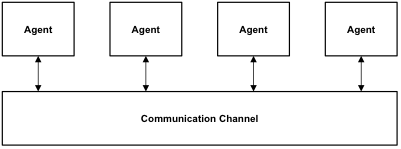
\includegraphics[scale=1, max size={\textwidth}{\textheight}]{SOA1}
\caption{Flat \gls{MAS} Architecture}
\label{SOA1}
\end{center}
\end{figure}

\item Fixed Hierarchy \gls{MAS} Architecture: Agents communicate only to agents directly above or below them in the hierarchy. Hierarchy is fixed leading to defects in systems scalability. Figure \ref{SOA2} presented in page \pageref{SOA2} depicts hierarchical \gls{MAS} architecture.

\begin{figure}
\begin{center}
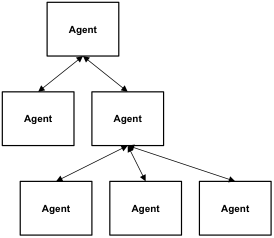
\includegraphics[scale=1, max size={\textwidth}{\textheight}]{SOA2}
\caption{Hierarchical \gls{MAS} Architecture}
\label{SOA2}
\end{center}
\end{figure}

\item Subsumption \gls{MAS} Architecture: Agent can contain other agents. Highly performance and wide scalability is the main advantage of subsumption architecture. Figure \ref{SOA3} presented in page \pageref{SOA3} shows subsumption \gls{MAS} architecture.

\begin{figure}
\begin{center}
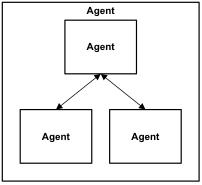
\includegraphics[scale=1, max size={\textwidth}{\textheight}]{SOA3}
\caption{Subsumption \gls{MAS} Architecture}
\label{SOA3}
\end{center}
\end{figure}

\item Modular \gls{MAS} Architecture: Agents are grouped in modules as presented in figure \ref{SOA4} presented in page \pageref{SOA4}. Communication takes place between agents composing the module, and agents of different modules. Each module is specified with one or more task(s). Presenting systems as collection of modules facilitated problem solving.

\begin{figure}
\begin{center}
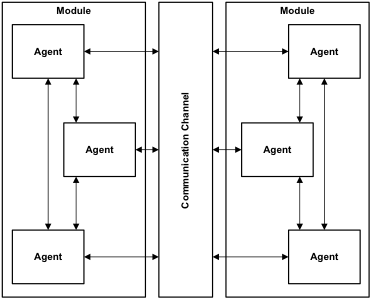
\includegraphics[scale=1, max size={\textwidth}{\textheight}]{SOA4}
\caption{Modular \gls{MAS} Architecture}
\label{SOA4}
\end{center}
\end{figure}

\end{itemize}
Multi-Agent architecture standards were attempted in order to force \gls{MAS} standardization and global integration. Knowledge Query and Manipulation Language (\gls{KQML}) was presented in order to support knowledge sharing among agents [125]. Knowledge Interchange Format (\gls{KIF}) is a computer-oriented language for the interchange of knowledge among disparate programs [126]. The OMG group proposed a reference model as an attempt to standardize the development of agent technologies [127]. \gls{KAoS} is described as "an open distributed architecture for software agents.'' The \gls{KAoS} architecture describes agent implementations, and elaborates on the interactive dynamics of agent-to-agent messaging communication by using conversation policies [128]. The Foundation for Intelligent Physical Agents (\gls{FIPA}) is a multi-disciplinary IEEE standardizing group pursuing the standardization of agent technology. \gls{FIPA}'s approach to \gls{MAS} development is based on a "minimal framework for the management of agents in an open environment'' [129]. Unfortunately, as a result for all the standardization effort, there were no universally accepted commercially supported standard yet.
\subsection{Webservices}
Web services are not just an integration solution. Web services technology is currently the major implementation of \gls{SOA} [130]. All service models are specific to the WS-Coordination specification and related protocols [99]. Web services adoption by organizations solved many problems. Web services is a general framework that expedites the sharing of heterogeneous data and software resources dispersed on the internet. The standard-based resource sharing and platform-neutral characteristics of web services have motivated many organizations to apply the technology in diverse areas, such as \gls{SCM}, virtual enterprise, homeland defense, e-government, and e-business [131]. Software agents can consume Web services as presented in [132].\index{Service Oriented Architecture}
\section{Webservices Technology}
Web services are applications that use standard transports, encoding, and protocols to exchange information [133]. A Web service is a software system designed to support interoperable machine-to-machine interaction over a network. Web service has an interface described in a format that machines can process (specifically \gls{WSDL}), Other systems interact with the Web service in a manner prescribed by its description using \gls{SOAP} messages, typically conveyed using \gls{HTTP} with \gls{XML} serialization in conjunction with other Web-related standards [134].
\subsection{Webservices Architecture}
Web service technology is based on open technologies; this provides broad interoperability among different vendor solutions [103]. Figure \ref{SOA5} presented in page \pageref{SOA5} shows the basic Web services architecture, that consists of specifications (\gls{SOAP}, \gls{WSDL}, and \gls{UDDI}) that support the interaction of a Web service requester with a Web service provider and the potential discovery of the Web service description [135]. The provider typically publishes a \gls{WSDL} description of its Web service, and the requester accesses the description using a \gls{UDDI} or other type of registry, and requests the execution of the provider's service by sending a \gls{SOAP} message to it.
\begin{figure}
\begin{center}
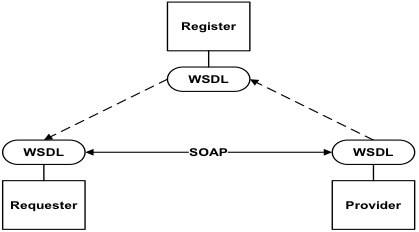
\includegraphics[scale=1, max size={\textwidth}{\textheight}]{SOA5}
\caption{Basic Webservices' Architecture}
\label{SOA5}
\end{center}
\end{figure}

Web service protocols cover all aspects of \gls{SOA}s, from the basic mechanisms for service information exchange (\gls{SOAP}) to programming language standards (WS-BPEL). These standards are all based on \gls{XML}, a human and machine-readable notation that allows the definition of structured data where text is tagged with a meaningful identifier. \gls{XML} has a range of supporting technologies, such as XSD for schema definition, which are used to extend and manipulate \gls{XML} descriptions. Erl (2004) provides a good summary of \gls{XML} technologies and their role in web services.\index{Service Oriented Architecture}
Briefly, the key standards for web \gls{SOA}s are as follows:
\begin{enumerate}
\item \gls{SOAP} This is a message interchange standard that supports the communication between services. It defines the essential and optional components of messages passed between services.
\item \gls{WSDL} is a standard for service interface definition. It sets out how the service operations (operation names, parameters, and their types) and service bindings should be defined.
\item WS-BPEL This is a standard for a workflow language that is used to define process programs involving several different services.
A service discovery standard, \gls{UDDI}, was also proposed but this has not been widely adopted. The \gls{UDDI}  standard defines the components of a service specification, which may be used to discover the existence of a service. These include information about the service provider, the services provided, the location of the \gls{WSDL} description of the service interface, and information about business relationships. The intention was that this standard would allow companies to set up registries with \gls{UDDI} descriptions defining the services that they offered.
\end{enumerate}

\subsection{Webservices Key Features}
Some of Web services key features are [103]:
\begin{itemize}
\item Self-contained: On the client side, a programming language with \gls{XML} and \gls{HTTP} client support is the only requirement. On the server side, a Web server and a servlet engine are required.
\item Self-describing: format and content of request and response messages (loosely coupled application integration) is what only matters. Messages are descriptive, not instructive.
\item Modular: Web services are a technology for deploying and providing access to business functions over the Web; J2EE, \gls{CORBA}, and other standards are technologies for implementing Web services.
\item Web published, located, and invoked: by applying the previously mentioned standards \gls{SOAP}, \gls{XML}, \gls{WSDL}, and \gls{UDDI}, Web services can be published, located, and invoked via internet.
\item Language independent: interaction between a service provider and a service consumer is designed to be completely platform and language independent. Interaction requires a \gls{WSDL} document to define the interface and describe the service, along with a network protocol (usually \gls{HTTP}). 
\item Interoperable: Because service provider and service consumer do not share same platforms or languages; only communicate via standard protocols, interoperability is achieved.
\item Inherently open and standards based: \gls{XML}, \gls{SOAP}, \gls{WSDL} and \gls{HTTP} are the technical foundation for Web services. A large part of the Web service technology has been built using open source projects. 
\item Dynamic: dynamic e-business can become a reality using Web services because, with \gls{UDDI} and \gls{WSDL}, the Web service description and discovery can be automated.
\item Composable: Web services can be aggregated to complex ones.
\end{itemize}
\subsection{Webservices Advantages}
Web services advantages arise from Web services key features. Web services were designed to satisfy all software requirements arose over the years, and avoid all drawbacks of previous technologies. Web services advantages include [133,136, 137, 138, 139]:
\begin{itemize}
\item Interoperability: Software interoperability is the capability to communicate, execute programs, or transfer data among various functional units in a manner that requires the user to have little or no knowledge of the unique characteristics of those units. Web services are interoperable.
\item Language agnostic: Web services are neither based on a programming language nor on a programming data model. Any Programming language can be used to implement Web services.
\item Relatively simple: Web services are simple to build, expose, and consume because they are:
\begin{itemize}
\item Based on Web technologies: so, they are scalable, and easily to control security features.
\item Do not necessarily require a huge framework in memory: A small amount of code could expose a service as a Web Service, besides Web services can be used easily in today's Web Interface. 
\end{itemize}
\item Loosely coupled applications: applications based on Web services are loosely coupled applications by default. Loose coupling is a design goal that describes a resilient relationship between two or more applications, systems, or organizations with some kind of exchange relationship [140]. In Web services, exchange relationship is established via request/response messages.
\item Support of software industry leaders: Hundreds of IT vendors have participated in the Web services standardization process under the sponsorship of the World Wide Web Consortium (\gls{W3C}), Organization for the Advancement of Structured Information Standards (OASIS) and Web Services Interoperability Organization (WS-I).  IT vendors include, not only: Microsoft, Oracle, bea, SAP, IBM, and Sun..
\item Integration with the World Wide Web: Web services tended to integrate with World Wide Web from the very first beginning in order to use internet as the infrastructure. Internet integration provides the most advantage of adopting Web services within applications.
\end{itemize}

\subsection{Enhanced Standards}
A number of companies, such as Microsoft, set up \gls{UDDI} registries in the early years of the 21st century but these have now all closed. Improvements in search engine technology have made them redundant. Service discovery using a standard search engine to search for appropriately commented \gls{WSDL} descriptions is now the preferred approach for discovering external services.
The principal \gls{SOA} standards are supported by a range of supporting standards that focus on more specialized aspects of \gls{SOA}. There are a very large number of supporting standards because they are intended to support \gls{SOA} in different types of enterprise application. Some examples of these standards include the following:\index{Service Oriented Architecture}
\begin{enumerate}
\item WS-Reliable Messaging, a standard for message exchange that ensures messages will be delivered once and once only.
\item WS-Security, a set of standards supporting web service security including standards that specify the definition of security policies and standards that cover the use of digital signatures.
\item WS-Addressing, which defines how address information should be represented in a \gls{SOAP} message.
\item WS-Transactions, which defines how transactions across distributed services should be coordinated.
\end{enumerate}
Current web services standards have been criticized as being ‘heavyweight’ standards that are over-general and inefficient. Implementing these standards requires a considerable amount of processing to create, transmit, and interpret the associated \gls{XML} messages. For this reason, some organizations, such as Amazon, use a simpler, more efficient approach to service communication using so-called RESTful services.

\subsection{RESTful Webservice}
The set of web services protocols that have been developed support a very general model of web services and have taken into account important enterprise issues such as security, reliability and transactions. They allow services from different providers to be dynamically linking and executed.

However, an inevitable consequence of this generality is that there is significant processing overhead in interpreting the \gls{XML} documents that are exchanged by web services. This can mean that the performance of service-oriented systems is reduced. This has led to alternative approaches to service implementation which use simpler protocols and which are usable in situations where the generality offered by 'big' web services is not required.

REST (REpresentational State Transfer) is an architectural style based on transferring representations of resources from a server to a client. It is the style that underlies the web as a whole and has been used as a much simpler method than \gls{SOAP}/\gls{WSDL} for implementing web services \cite{SWE9}.
A RESTful web service is identified by its URI (Universal Resource identifier) and communicates using the HTML protocol. It responds to HTML methods GET, PUT, POST, and DELETE and returns a resource representation to the client. Simplistically, POST means create, GET means read, PUT means update, and DELETE means delete.
RESTFul services involve a lower overhead than so-called ‘big web services’ and are used by many organizations implementing service-based systems that do not rely on externally provided services.

So-called RESTful web services follow the REST (REpresentational State Transfer) architectural style, with all communications based on the simple \gls{HTTP} protocol. Services are modeled as resources (e.g. a parts catalogue) and respond to \gls{HTTP} methods GET, POST, PUT and DELETE. The service is addressed using its URI (Universal Resource Identifier.

The information exchanged by RESTful services is the resource representation which may be \gls{XML}, but, in principle, other representations such as JSON (Javascript Object Notation) may also be exchanged.

The \gls{HTTP} methods are usually interpreted as \cite{RESTful}:
\begin{itemize}
\item POST=Create
\item GET = Read
\item PUT = Update or Create
\item DELETE = Delete
\end{itemize}
The key benefit of RESTful services is that they are simpler and more efficient than 'Big' web services. The amount of processing overhead is reduced, which is particularly important for simple services than implement small increments of functionality.

\gls{SOAP} and REST are not incompatible and it is possible for web services providers to offer both \gls{SOAP} and REST service interfaces. Major providers such as Amazon offer both and their experience is that the REST interface is often preferred by developers.

\section{An in-car Information System}
\gls{SOA}s are loosely coupled architectures where service bindings can change during execution. This means that a different, but equivalent version of the service may be executed at different times. Some systems will be solely built using web services and others will mix web services with locally developed components. To illustrate how applications that use a mixture of services and components may be organized, consider the following scenario:
An in-car \gls{IS} provides drivers with information on weather, road traffic conditions, local information, and so forth  \cite{SWE9}. This is linked to the car radio so that information is delivered as a signal on a specific radio channel. The car is equipped with GPS receiver to discover its position and, based on that position, the system accesses a range of information services. Information may then be delivered in the driver’s specified language.
Figure \ref{SOAincar} presented in page \pageref{SOAincar} illustrates a possible organization for such a system. The in-car software includes five modules. These handle communications with the driver, with a GPS receiver that reports the car’s position and with the car radio. The Transmitter and Receiver modules handle all communications with external services.\index{Service Oriented Architecture}
The car communicates with an external mobile information service that aggregates information from a range of other services, providing information on weather, traffic information, and local facilities. Different providers in different places offer these services, and the in-car system uses a discovery service to locate appropriate information services and bind to them. The discovery service is also used by the mobile information service to bind to the appropriate weather, traffic, and facilities services. Services exchange \gls{SOAP} messages that include GPS position information used by the services to select the appropriate information. The aggregated information is then sent to the car through a service that translates that information into the driver’s preferred language.
\begin{figure}
\begin{center}
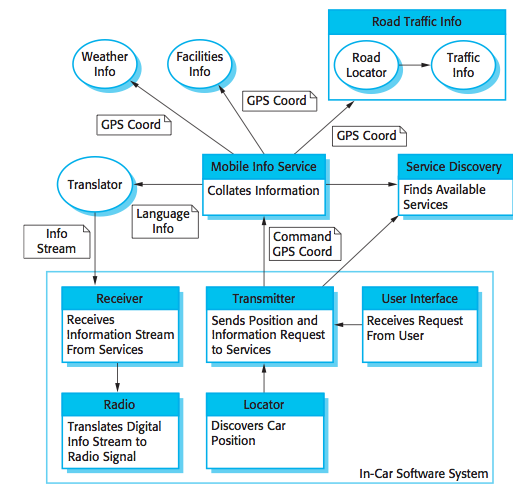
\includegraphics[scale=.8, max size={\textwidth}{\textheight}]{SOAincar}
\caption{Service-based in-car \gls{IS} \cite{SWE9}}
\label{SOAincar}
\end{center}
\end{figure}


\section{Webservices as SOA enabler}
\index{Service Oriented Architecture}
Web services are relatively new technology that have received wide acceptance as an important implementation of \gls{SOA} [103]. Web services is not \gls{SOA}, and \gls{SOA} is not Web services. It is important to differentiate between Web services; as a technology, and \gls{SOA} as a design pattern. Web services enabled the maximum advantages of \gls{SOA}, this is mainly why Web services is the main implementation and enabler of \gls{SOA}. \gls{SOA} presents systems as collection of services to be published, and consumed when required. When exposed services are Web services, system gains the advantage of Web services standardization, like interoperability. But still systems need to be studied carefully, and analyzed intensively to determine services will be exposed, suitable services interfaces, and design the required databases. \gls{SOA} is not about exposing and consuming Web services to facilitate interoperability or integration or other requirements, but it is rather the science, art, and practice of building loosely coupled fine granular services to form applications.

\section{Enterprise Service Bus}
\gls{ESB} provides a comprehensive, scalable way to connect a large number of applications without the need for each pair of applications to make a direct connection. Such a direct connection between two applications is called a point-to-point connection. Note that even in the case of Web Services, the connection between the service consumer application and the service provider application is “point to point.” The point-to-point connection approach does not scale well because the number of applications involved in the integration increase; therefore, this integration approach is not suitable for a large enterprise where a large number of applications need to be integrated.

\subsection{ESB}
\gls{ESB} can be defined in two contexts: design and run-time. As a design-time context, \gls{ESB} is an architectural pattern that has multiple motivations:
\begin{itemize}
\item Supports large numbers of service interactions in a manageable way
\item Provides support for advanced service interaction capability, such as transactions, store and forward, infrastructure services, security, quality of service, and so on
\item Supports a variety of interaction styles such as synchronous request/response, messaging, publish/subscribe, and events
\item Provides a robust, manageable, distributed integration infrastructure consistent with the principles of \gls{SOA}
\item Supports service routing and substitution, protocol transformations, and other message processing
\item Supports both Web Services and traditional \gls{EAI} communication standards and technologies
\end{itemize}
The ESB pattern can be implemented in one or more of the following hybrids:
\begin{itemize}
\item \gls{EAI} technology
\item Messaging technology
\item Technology rebranded or classified as an ESB product 
\item “Gateway” technology
\item Appliance technology
\item Bespoke
\end{itemize}
The \gls{ESB} mediates characteristics of interactions between service requestors and service providers. The ESB enables the substitution of service providers or implementations transparent to service requesters. The ESB supports a variety of means to attach requesters and providers, and it allows intermediary services to be sequenced between requesters and providers. The \gls{ESB} may provide a broad set of capabilities dependent on business needs and implementation in several areas, including network communications, integration, security, message processing, quality of service, and service management.
\subsection{ESB vs. Integration Technology}
An ESB is a connectivity infrastructure for integrating applications and services, in contrast to \gls{EAI}, which focuses on the integration of applications. ESB infrastructure differs from \gls{EAI} in the following aspects:
\begin{itemize}
\item ESB infrastructure is more than integration because it performs routing of messages between services, converts transport protocols between consumers and providers, transforms message formats between requesters and providers, and distributes
business events from disparate sources. Although \gls{EAI} solutions can address all of these aspects, integration technologies are usually much more narrowly focused. ESB handles a variety of interaction patterns, including events.
\item ESB requires management such that the status of a business transaction can be assessed. Has the transaction completed? How long did it take? Did the process step complete? Although the ESB will not be the only technology to assist in business activity management, it will be a part.
\item ESB product technologies will be federated such that various technologies (e.g., gateways and appliances) can be used to fulfill a single purpose and provide a single interface to applications. Heterogeneous platforms can be supported allowing different ESB technologies to operate as a single logical ESB.
\end{itemize}

\subsection{ESB Functionality}
Business-and IT-level events are used by service-level automation to enforce the policies associated with the business services they host. A service bus can be used to collect, aggregate, and evaluate those events for presentation to business process participants in business activity management scenarios. The ESB provides a broad set of capabilities dependent on scenarios:
\begin{itemize}
\item Communications: Routing, addressing, protocol, publish/ subscribe interactions, asynchronous interactions, event handling, and other features.
\item Service Interaction: Interface definition, \gls{SOA}P, REST, and other features
\item Integration: \gls{DB}, legacy, and middleware connectivity; service aggregation, application server connectivity, protocol transformation, and other features
\item Quality of Service: Transactions and delivery assurance, and other features
\item Security: Authentication, authorization, non-repudiation, confidentiality, standards support, and other features
\item Service level: Performance, throughput, availability, scalability, and other features
\item Message Processing: Message and data transformations, intermediaries, content-based routing, and other features
\item Management and Autonomic: Service provisioning and registration, logging, metering, monitoring, system management, and other features
\item Appliances: Parsing, compression, routing, and other features
\item Infrastructure Intelligence: Business rules, policy-driven behavior, pattern recognition, and other features
\end{itemize}

\subsection{BizTalk Server}
Microsoft BizTalk Server uses adapter technology to connect disparate entities and enable the integration of data, events, processes, and services. An entity may be an application, department, or even an altogether different organization that needed to be able to share information with. A software adapter is typically used when we need to establish communication between two components that do not natively collaborate. BizTalk Server adapters are built with a common framework which results in system integration done through configuration, not coding. Traditionally, BizTalk Server has solved problems in three areas. First, BizTalk Server acts as an \gls{EAI} server that connects applications that are natively incapable of talking to each other. The applications may have incompatible platforms, data structure formats, or security models. For example, when a new employee is hired, the employee data in the human resources application needs to be sent to the payroll application so that the new employee receives his/her paycheck on time. Nothing prevents you from writing the code necessary to connect these disparate applications with a point-to-point solution. Many organizations choose to insert a communication broker between these applications. Some of the benefits that you would realize from such an architectural choice include:
\begin{itemize}
\item Loose coupling of applications where one does not have a physical dependency on the other
\item Durable infrastructure that can guarantee delivery, and queue messages during destination system downtime
\item Centralized management of system integration endpoints
\item Message flow control such as in-order delivery
\item Insight into cross-functional business processes through business activity monitoring
\end{itemize}
BizTalk Server solves a second problem by filling the role of business-to-business (B2B) broker that facilitates communication across different organizations. BizTalk supports B2B scenarios by offering Internet-friendly adapters, industry-standard EDI message schema, and robust support for both channel- and message-based security.
The third broad area that BizTalk Server excels in is Business Process Automation (BPA). BPA is all about taking historically manual workflow procedures and turning them into executable processes. For example, consider the organization that typically receives a new order via email and the sales agent manually checks inventory levels prior to inserting the order into the Fulfillment System. If inventory is too low, then the sales agent has to initiate an order with their supplier and watch out for the response so that the Inventory System can be updated. 

\section{SOA Selected Topics}
\subsection{SOA service vs. Webservice}
\gls{SOA} services can be realized as web services, but not all web services are equal to \gls{SOA} services. Web services represent the use of both a published standard and a set of technologies for invocation and interoperability. \gls{SOA} services are services that fulfill a key step or activity of a business process and can be described as business services and are often exposed as web services.
We can distinguish between \gls{SOA} service and Webservice in design time, and runtime.
\begin{itemize}
\item In design, we identify and specify a service that provides the design, or we identify and specify interfaces that include method specifications. The combination of the definition of the method and the interface at design time is what we refer to as a service from an \gls{SOA} perspective. Use cases can be used to capture the functional requirements for a service.
\item In runtime, In an \gls{SOA}, business processes, activities, and workflow are broken down into constituent functional elements called services. They can be accessed and used directly by applications, or they can be mixed and matched with other services to create new business capabilities. Business services or \gls{SOA} services are reusable business capabilities. Examples in banking include open account or change address. For transportation, it might be get reservation or hold reservation, and with loan processing, get loan, apply for loan, and update address are examples of business services.
\end{itemize}
\subsection{SOA vs. DCE and CORBA}
The difference between \gls{SOA} and earlier approaches, such as \gls{DCE} or \gls{CORBA}, has a lot to do with standardization. This was initially brought about through the use of Web services and Web services standards. \gls{WSDL}, \gls{SOAP}, and other Web services standards enable the industry to converge around a common infrastructure model for runtime. Different vendors would have different implementations, but they would generally conform to the base models. The Web Services Interoperability Organization (WS-I) is an example of an effort to pull things together so that different vendor implementations are consistent and compliant to the degree possible. Web services, unlike earlier approaches, built upon existing and deployed infrastructure as it took advantage of the Internet, resulting in less cost for adoption and reduced risk.
Agreed upon versus \textit{defacto} standards is a huge difference between \gls{SOA} and earlier approaches. Web services standards have been the genesis of \gls{SOA}, and Web services are more language independent than object-oriented technology integration approaches, which are often language specific (e.g., Java, C, or Smalltalk). \gls{XML} is language neutral and renders naturally into languages of choice: COBOL, C++, Java, or others. \gls{XML} and Web services standards, such as \gls{WSDL}, have improved flexibility than approaches such as \gls{CORBA} or \gls{RPC} found in \gls{DCE}, where changes and additions to the data structures often resulted in breakages of the code that used such structures. In contrast, \gls{XML} does not use offsets, and it is therefore possible to reorder or add data elements without a break in older versions. Web services also use one type space for interfaces, and that type is \gls{XML}. The other approaches use one type for databases (e.g., SQL), another for in-flight messages (e.g., Internet Inter-Orb Protocol, IIOP), and another Interface Definition Language (IDL; e.g., CORBA). One approach versus three creates an easier-to-use developer toolkit and application programming interface (API) set, and it makes the code base less brittle and easier to change. Contracts that provide a valid sequence of interaction with a service and policies that govern the nonfunctional characteristics of a service have augmented the notion of the interface found in earlier approaches.
One of the most important advances that \gls{SOA} provides is that the set of services that are required by organizations and captured in the service portfolio provides a business language between business and IT to discuss fulfillment of business needs. A service portfolio is governed as an enterprise asset and used by business and IT stakeholders. This represents a big change from CORBA and \gls{RPC}, which are something IT uses. \gls{SOA} and services provide much more than programmatic notions; they provide services at a granularity that the business understands and can use.

\subsection{SOA vs. CBA}
The differences between a service-oriented approach and a component-oriented approach to distributed systems architectures are \cite{SOAvsCBA-1}:
\begin{enumerate}
\item Services can be offered by any service provider inside or outside of an organization. Assuming these conform to certain standards (discussed below), organizations can create applications by integrating services from a range of providers. For example, a manufacturing company can link directly to services provided by its suppliers.
\item The service provider makes information about the service public so that any authorized user can use the service. The service provider and the service user do not need to negotiate about what the service does before it can be incorporated in an application program.
\item Applications can delay the binding of services until they are deployed or until execution. Therefore, an application using a stock price service (say) could dynamically change service providers while the system was executing.
\item Opportunistic construction of new services is possible. A service provider may recognize new services that can be created by linking existing services in innovative ways.
\item Service users can pay for services according to their use rather than their provision. Therefore, instead of buying an expensive component that is rarely used, the application writer can use an external service that will be paid for only when required.
\item Applications can be made smaller (which is important if they are to be embedded in other devices) because they can implement exception handling as external services.
\item Applications can be reactive and adapt their operation according to their environment by binding to different services as their environment changes.
\end{enumerate}

\subsection{WSDL vs. REST}
\gls{SOA} is an architectural style, and that the use of Web services is only one way to implement or realize this architectural style. In fact, there may be a set of different implementations of a service portfolio. Suppose, for instance, that the service portfolio has 100 services; 50 of them may be implemented using Web services, and the rest may be implemented using a combination of Representation State Transfer (REST) and Simple Object Access Protocol (\gls{SOAP}). Or, an architectural decision can be made to use other Java or .NET mechanisms that do not use REST or \gls{SOAP}. \gls{SOA} does not constrain a solution to using Web services, \gls{SOAP}, or REST. However, using Web services is a best practice, and using \gls{WSDL} is the fundamental aspect of what makes a Web service not \gls{SOAP} or REST. There are different patterns for \gls{SOA} implementation patterns. Not all of them promote \gls{SOA} best practices. Pattern 1 is a tightly coupled interaction, which does not use a Services Layer but may use a service interface in the operational system. In this pattern, it’s unlikely that \gls{SOAP} or REST is used, and most likely a proprietary messaging interface is the transport of choice. In pattern 2, a service component is used with a service interface but no Services Layer is in place. In pattern 3, a Services Layer is present, but the service maintains state in its interactions with the service component and Operational Systems Layer. In pattern 4, a packaged solution provides a service interface and most likely makes REST or \gls{SOAP} options available. In pattern 5, a business state machine might be in use directly interacting with service interfaces. In pattern 6, a Business Process Layer and Services Layer are leveraged. The primary reason for illustrating the various \gls{SOA} interaction patterns is to illustrate that there is no right or wrong choice when picking \gls{SOAP} or REST. Instead, choices may be architecturally weak or strong based on the interaction pattern needed, the quality of service (QoS) attributes that must be achieved, the examination of any constraints imposed by existing operational systems, and the determination of where the greater flexibility lies. One can then make an architectural choice: \gls{SOAP}, REST, or another interaction. The use of \gls{SOAP} often is equated as using Web services when in fact Web services can also be REST-based Web services. In \gls{SOA} adoption, the interaction patterns are architectural decisions along with whether to use \gls{SOAP}, REST, or other service.

\subsection{Fundamental Types of Services}
There are three fundamental types of service that may be identified \cite{BS58}:
\begin{enumerate}
\item Utility services These are services that implement some general functionality that may be used by different business processes. An example of a utility service is a currency conversion service that can be accessed to compute the conversion of one currency (e.g., dollars) to another (e.g., euros).
\item Business services These are services that are associated with a specific business function. An example of a business function in a university would be the registration of students for a course.
\item Coordination or process services These are services that support a more general business process which usually involves different actors and activities. An example of a coordination service in a company is an ordering service that allows orders to be placed with suppliers, goods accepted, and payments made.
\end{enumerate}

\subsection{REST}
REST is an architectural style that uses the analogy of the state transition diagram and maps that to an application having a set of resources that are connected by state transitions or links. A network of nodes such as the World Wide Web provides an ability to click a link and be transferred to the resource for that link. For example, if you are on a Web page that is a representation of a resource, you are then considered to be in a particular state when you are on that Web page. By clicking a link within that initial Web page that represents the current state, you convey the intent to transition to another Web page, which is really a resource representation of the next state. Thus, a network of states and transitions is traversed by selecting the appropriate link to the appropriate resource. This resource representation puts you, accessing the resource, into a particular state. When you click a link on that page, you get a representation of another resource. When you continue to access various resources by following the links, you keep changing state. This is essentially what is meant by REST.
\subsection{Web services vs. REST}
There are three main differences between Web services and REST:
\begin{itemize}
\item Service oriented versus resource oriented. With Web services, you are requesting a service (and so this is service oriented). With REST, however, you are implying you are looking for a specific type of resource (and so this is considered to be resource oriented).
\item Use of \gls{HTTP}. REST typically uses \gls{HTTP} as the transport, whereas \gls{SOAP} has no restriction on the use of a particular transport. Many people use REST-style interactions using \gls{HTTP}.
\item Quality of service. When you use REST, all the QoS parameters must be provided by the transport itself. In Web services, a significant number of specifications must be written to support QoS options, using the WS-*set of standards.
\end{itemize}

\section{Summary}
A web service is an instance of a more general notion of a service, which is defined as:
“an act or performance offered by one party to another. Although the process may be tied to a physical product, the performance is essentially intangible and does not normally result in ownership of any of the factors of production”. The essence of a service, therefore, is that the provision of the service is independent of the application using the service. Service providers can develop specialized services and offer these to a range of service users from different organizations. \gls{SOA} are a way of developing distributed systems where the system components are stand-alone services, executing on geographically distributed computers. Standard \gls{XML}-based protocols, such as \gls{SOAP} and \gls{WSDL}, have been designed to support service communication and information exchange. Consequently, services are platform and implementation-language independent. Software systems can be constructed by composing local services and external services from different providers, with seamless interaction between the services in the system. This chapter presented different topics related to \gls{SOA}, including: \gls{SOA} advantages, technologies, different methods of implementation, examples of \gls{IS} based on \gls{SOA}, and concluded with an important concept, that is \gls{ESB}.

\section{Review Questions}
\begin{enumerate}
\item What is \gls{SOA}?
\item What are \gls{SOA} advantages?
\item What are \gls{SOA} main technologies?
\item What is Webservice?
\item What are Webservices advantages?
\item What is Webservice Enhanced Standards?
\item What is \gls{ESB}?
\item What is REST?
\item What are the fundamental types of Services?
\end{enumerate}

\section{Exercises and Labs}
In Labs, you shall be getting familiar with Java programming language, as it is the programming language we will be using to build, deploy, and consume different online Webservices and \gls{SOA} systems presented in this book.


\chapter{BPM and SOA}
\label{BPMandSOA}
\section{Introduction}
Business Agility is a relatively new paradigm painted as a solution for maintaining competitive advantage during times of uncertainty and turbulence in the business environment \cite{BS01}. Business improvement approaches, such as Total Quality Management (TQM), Business Process Reengineering (BPR), and Workflow Management Systems (WfMS) failed to satisfy business agility requirements due to different reasons. Three approaches realized the need for \gls{BPM} \cite{BS02}. Business process is a series of inter-related activities that cross functional enterprise boundaries with individual inputs and outputs \cite{BS03, BS04}. \gls{BPM} is a systematic, structured approach to analyze, improve, control, and manage processes \cite{BS02}. \gls{BPMS} is an \gls{EIS} that supports designing, administrating, and improving the business processes \cite{BS05}. \gls{EIS}s suffer from lack of agility and inefficiency \cite{BS06}. \index{Enterprise Information System} Lack of agility refers to enterprises inability to match business requirements, especially new ones, onto current IT infrastructure and \gls{IS}s architecture. Inefficiency refers to the \gls{IS}s development process that costs too much when compared to the actual output. \gls{SOA} as a design pattern presents IT infrastructure and \gls{IS}s architecture as loosely coupled, fine granular services that can address business requirements once they are presented either by adding new services or modifying existing ones. \gls{SOA} also addresses enterprises information systems inefficiency by enhancing reusability, thus theoretically, shortening \gls{IS}s development time and effort required. Two main approaches for designing and implementing \gls{SOA} based \gls{IS}s are software agent based \gls{SOA}, and Web services based \gls{SOA}. Both approaches are presented in this chapter.

This chapter goes as follows: section two presents business agility principles, and framework. Section three presents business process aspect of business agility, and the need for \gls{BPMS}. Section four presents \gls{SOA} as the solution to technical agility as one of business agility aspects. Section five presents the proposed model aligning \gls{BPMS} and \gls{SOA} highlighting potential enterprises’ benefits and advantages of this align regarding business agility.  

\section{Business Agility}
Business agility is a concept that extends adaptability and flexibility to include speed and scalability \citep{W28}. Adaptability is the opportunity for \gls{EIS} adaptation to different specified environments without applying other actions or means than provided for this purpose. \index{Enterprise Information System} Flexibility is the ability of an \gls{EIS} to respond to potential internal or external changes affecting its value delivery, in a timely and cost effective manner \citep{M38}. Scalability refers to the ease with which an \gls{EIS} can be modified to fit the problem area. Anarchic scalability defines the need for architectural elements to continue operating when they are subjected to an anticipated load, or when given malformed or maliciously constructed data, since they may be communicating with elements outside enterprises control \citep{EV05}. Business Agility is the term applied to an organization's ability to react to unanticipated market change, defining informed rapid transformation of organizational process and product \citep{BS10}. Business Agility is the ability to sense change and opportunity in the marketplace, respond quickly, and execute successfully. Business agility is the sustained ability to sense and respond to change after change, executing well, occasionally inflicting change on competitors, yielding market leading returns \citep{BS11}. Agile enterprise is the enterprise capable of responding quickly to changes \citep{BS12}.

Business agility is a promising strategy in times of change and uncertainty \citep{W28}. Enterprises must increasingly be organized, managed, and executed in ways that allow them to effectively sense and respond to unpredictable events in their environment. Enterprises must demonstrate agility in order to stay competitive \citep{BS13}. Business change is inevitable, and whatever organizational framework is developed, it needs to be flexible to change \citep{W27, BS15}.

\subsection{Business Agility Principles}
Business agility principles can be extracted from different approaches of adaptive organizations \cite{BS16}. Adaptive organizations are organizations that get affected by the social characteristics of its participants as well as the varied pressures imposed by its environment \cite{BS17}. There are many approaches for adaptive organizations, like Haeckel’s approach. Business agility principles include \cite{BS16,BS18}:
\begin{enumerate}
\item Agile enterprise entities must address four main agility characteristics:
\begin{itemize}
\item Cooperate to enhance competitiveness.
\item Enrich the customer.
\item Master change and uncertainty.
\item Leverage the impact of people and information.
\end{itemize}
\item Traditional \gls{EIS}s that work well in stable predictable environment is replaced with adapted \gls{EIS} with specific governance mechanism. \index{Enterprise Information System}
\item Translation of enterprise mission and practices into information that can be communicated and interpreted.
\item Each business process should have dimensions that manage its relationship with other different enterprise entities.
\item Enterprise needs to implement business process lifecycle on different levels. Business process lifecycle is one of \gls{BPM} promises about business process processing. Business process lifecycle phases include: model, design, simulate, execute, monitor, and optimize \cite{BS19}.
\item Enterprise needs to implement mechanisms for business process learning on different levels. Everyone in the enterprise should have access to the same business processes repository. The repository is used to support quality, definition of information requirements, and \gls{BPM} modeling \cite{BS20}.
\end{enumerate}

\subsection{Business Agility Framework}
Business agility means fast reaction to change and the ability to rapidly implement changes. Business agility needs to be holistic in scope \cite{W27}. Figure \ref{BS1} presented in page \pageref{BS1} presents business agility framework core components. Business agility consists of three interoperable components: Human, Business Process, and Technical agility. Humans are assumed to be agile in management and operations for the enterprise to be agile. Human agility is the main enabler of business agility. Business process agility has gone long road till it reached \gls{BPM} \cite{BS19}. \gls{BPMS} is the \gls{EIS} that realizes \gls{BPM}. Technical agility, that addresses IT infrastructure and \gls{IS}s architecture, can make use of \gls{SOA}. Aligning \gls{BPMS} and \gls{SOA} can enhance business agility. \index{Enterprise Information System}

\begin{figure}
\begin{center}
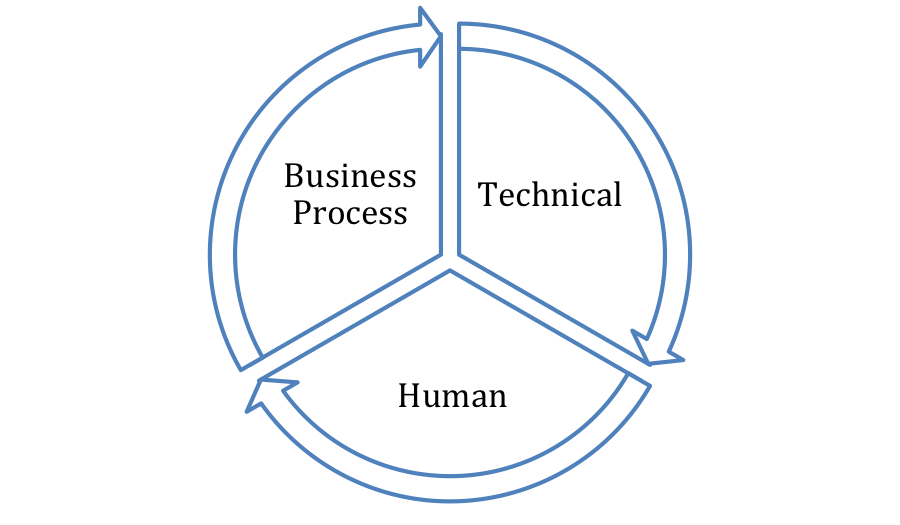
\includegraphics[scale=1, max size={\textwidth}{\textheight}]{BS1}
\caption{Business Agility Framework Components}
\label{BS1}
\end{center}
\end{figure}

\section{Business Process Agility}
\gls{BPM} (\gls{BPM}) is the key to business agility \cite{BS19}. Business process is a series of inter-related activities that cross functional enterprise boundaries with individual inputs and outputs \cite{BS03,BS04}. Business processes are either operational or supporting \cite{BS21}. Operational business processes are associated with the way enterprise develop strategies, invent, market and sell products or services. Support processes include the provision of Human Resource Management (HRM) activities, \gls{IS}s infrastructure, and finance and asset management. \gls{BPM}, as one of business improvement approaches, has a number of predecessors that include TQM, BPR, and WfMS. \gls{BPM} predecessors have realized the need for process management \cite{BS02}.

\subsection{TQM}
\gls{TQM} wave as a business improvement approach has risen at the late 1980s \cite{BS19}. TQM is a management approach for an organization, centered on quality, based on the participation of all its members and aiming at long-term success through customer satisfaction, and benefits to all members of the organization and to society \cite{BS22}. Unfortunately, quality is neither easily defined nor measured. TQM does not have a firm measure by which progress can be monitored. Quality must be converted into something more tangible to be measured, but this does not take place with TQM. Further, TQM does not introduce a clear path to follow.

\subsection{BPR}
\gls{BPR} as a business improvement approach has emerged in the early 1990s \cite{BS06}. BPR promised deliver of dramatic business improvements in a relatively short period of time by completely reinventing existing business processes that is, starting from scratch with new, optimized ways of doing business throwing out the old, encrusted, inefficient procedures of the past \cite{BS06,BS19}.   Unfortunately BPR involved lot of manual work, failed to provide agility or support ongoing change, could not adequately represent the full complexity of processes due to dependence on computer systems, and provided process discovery and design only in team meetings.

\subsection{WfMS and BPR}
\gls{WfMS} and \gls{ERP} promised Chief Executive Officer (CEO) the most flexible IT and providing enterprises requirements via software packages. Unfortunately, software packages were not flexible, installation could take months/years, subsequent applications couldn't be configured to meet all business requirements, business users were enforced to add components. Business process mapping Tools were added to ERPs, and WfMSs promising to produce documentation about the way company works, and to assist review and refinement of business process descriptions, but business process mapping tools could not carry business process models to execution, used proprietary formats and incompatible notations, focused mainly on modeling input-output activities and dataflow, with no focusing on collaborative activity aspect or processes complexity.

\subsection{BPM}
\gls{BPM} is the art of understanding, codifying, automating, and improving the way a company does business \cite{BS04}. \gls{BPM} is a systematic, structured approach to analyze, improve, control, and manage processes \cite{BS02}. \gls{BPM} promises that Processes viewed by human as information and machines as executable code, Process design precedes both from top down - at the level of business strategy and business process design - and bottom up - at the level of leveraging existing IT systems, Process design is reflected directly in the IT infrastructure, leverage existing investments by connecting databases, legacy systems and package solutions into flexible end-to-end business processes. \gls{BPM} introduces the concept of 'process processing' and stresses that this concept is not limited to the automatic execution of digital process models, but 'encompasses the discovery, design, and deployment of business processes, as well as the executive, administrative, and supervisory control over them to ensure that they remain compliant with business objectives' \cite{BS06,BS23}.

\subsection{BPMS}
\gls{BPMS} enables enterprises to realize \gls{BPM} initiatives \cite{BS05}. \gls{BPMS} is a revolutionary \gls{IS} that supports designing, administrating, and improving the business processes systematically. \gls{BPMS} is applied to create, execute, and optimize the business process model that powers the life cycle of each business process instance \cite{BS24}. \gls{BPMS} can be used to manage people-to-people, machine-to-machine, machine-to-people, and people-to-machine interactions \cite{BS25}.
\subsubsection{BPMS Key Features}
\gls{BPMS} will bring all the benefits of integration, flexibility, end-to-end visibility and control to the whole extended enterprise. \gls{BPMS} key features include:
\begin{itemize}
\item \gls{BPMS} integrates and orchestrates other IT systems: \gls{BPMS} will connect existing communication systems together, convey the required messages from one business entity to another, and ensure that the supply chain constituents stay aligned, with the system putting all of these interactions in the context of a whole process.
\item \gls{BPMS} connects and integrates existing databases, legacy systems, and package solutions into flexible end-to-end business processes.
\item Allows processes to be shared across \gls{BPMS} and across business boundaries: the use of a standard language for describing all aspects of a process will allow the same model to be deployed on several different systems.
\end{itemize}

\section{Technical Agility}
Technical agility refers to the ability to quickly change the type and flow of information within an organization within enterprise. Technical agility parameters are IT infrastructure, and \gls{IS} architecture. IT advance has not yet satisfied business requirements due to improper \gls{IS}s architectures. \gls{SOA} addresses technical agility requirements by presenting composability, modularity, and loose coupling concepts as services that wrap underlying IT infrastructure, databases, and legacy systems and present them via standard interface. There is a need to stabilize IT infrastructure rather than developing new ones \cite{W28} and \gls{SOA} enables this stabilization. Enterprises should balance IT to become better positioned and more agile [26]. Services are the building Blocks of an agile enterprise \cite{W30}. 

\gls{W3C} defines Service as ‘A Component capable of performing a task’. Service is ‘A vehicle by which a consumer’s need or want is satisfied according to a negotiated contract (implied or explicit) which includes Service Agreement, Function Offered and so on’ \cite{BS28}. \gls{SOA} is the design pattern that utilizes services concept to achieve architectural advantages. \gls{W3C} defines \gls{SOA} as ‘A set of components which can be invoked, and whose interface descriptions can be published and discovered’. This definition can be expanded to include the science, art and practice of building applications [29]. \gls{SOA} is defined as ‘The policies, practices, frameworks that enable application functionality to be provided and consumed as sets of services published at a granularity relevant to the service consumer. Services can be invoked, published and discovered, and are abstracted away from the implementation using a single, standards based form of interface’ \cite{BS28}. 

IT Benefits of adopting \gls{SOA} include \gls{EIS}s capabilities of \cite{BS30,BS31}: \index{Enterprise Information System}
\begin{itemize}
\item Avoid effect(s) of service provider change of implementation as a result of using standard interface.
\item Choose alternative instance of same service type without modifying requesting \gls{IS}.
\item Implement different technologies than partners. Implementation of standard interface enables integration and interoperability.
\item Increase services exposed in a loosely coupled manner, so \gls{IS}s can easily combine existing services, and new ones based on business needs. This means less duplication of resources and more potential for reuse.
\item Leverage existing legacy applications by wrapping them with standard interface.
\end{itemize}

\subsection{SW Agents as SOA implementation}
Different \gls{SOA} implementations using different software agents and mobile agents were presented \cite{BS13, BS32, BS33, BS34, R43}. One or more agent can perform a certain task; tasks can be thought as services that compose \gls{SOA}. Unfortunately, certain limitations inhibited software agents from being the widely accepted \gls{SOA} implementation. Software Agent is a computer system that is situated in some environment and is capable of autonomous actions in this environment in order to meet its design objectives \cite{BS36, BS37}. 

Software Agents have characteristics that make them suitable to perform complex functionality. Characteristics include: Autonomy, Interactivity, Reactivity, Proactivity, Intelligence, and Mobility \cite{MNAS02}. Agent is autonomous; it is capable of acting on its own. An agent is goal oriented, collaborative, and flexible, so, it must be autonomous. Agents are designed to interact with other agents, humans, or software programs (Interactivity). Instead of making a single agent conduct several tasks, additional agents can be created to handle un-delegated task. Agents perceive environment via preceptors \cite{BS39} and respond to changes (Reactivity). Agents do not just act in response to their environment, but agents are able to exhibit goal-directed behavior by taking an initiative (proactive). Agent may need mobility to work on different machines. An agent with this capability is called mobile agent, it can transport itself across different system architectures and platforms, and is far more flexible than those that cannot. Many electronic commerce agents are mobile \cite{MNAS02,BS40}. Mobile agent is an executing program that can migrate during execution from machine to machine in a heterogeneous network \cite{BS37}.

Multi-Agent Systems (MASs) are becoming increasingly important: as a scientific discipline, as a software engineering paradigm, and as a commercially viable and innovative technology \cite{BS41}. A Multi Agent is any system that contains \cite{BS42}:
\begin{itemize}
\item Two or more agents;
\item At least one autonomous agent; and
\item At least one relationship between two agents where one satisfies goal of the other.
\end{itemize}
Some of Multi-Agent frameworks proposed from 2005 till now include work presented in \cite{BS43, BS44, BS45, BS46, BS47, BS48}. Multi-Agent architecture standards were attempted in order to force \gls{MAS} global integration \cite{BS49}. Knowledge Query and Manipulation Language (\gls{KQML}) was presented in order to support knowledge sharing among agents \cite{BS50}. Knowledge Interchange Format (\gls{KIF}) is a computer-oriented language for the interchange of knowledge among disparate programs developed by the Advanced Research Projects Agency (\gls{ARPA}) sponsored Knowledge Sharing Effort \cite{R41}. The OMG group proposed a reference model as an attempt to standardize the development of agent technologies \cite{R42}. Knowledgeable Agent-oriented System (\gls{KAoS}) is described as "an open distributed architecture for software agents.'' The \gls{KAoS} architecture describes agent implementations (starting from the notion of a simple generic agent, to role-oriented agents such as mediators and matchmakers), and elaborates on the interactive dynamics of agent-to-agent messaging communication by using conversation policies [53]. The Foundation for Intelligent Physical Agents (\gls{FIPA}) is a multi-disciplinary IEEE standardizing group pursuing the standardization of agent technology. \gls{FIPA}'s approach to \gls{MAS} development is based on a "minimal framework for the management of agents in an open environment.'' \cite{BS54}. Unfortunately as a result for all the standardization effort, there were no universally accepted commercially supported standard yet. Software agents are not the main \gls{SOA} enabler because:
\begin{itemize}
\item Problems not easily defined into \gls{MAS} organizations
\item Absence of unified framework
\item Security is a very big concern, specially with mobile agents
\item Lack of commercial support
\item Semantic web and Web services presentation (availability) as alternative technologies
\end{itemize}

\subsection{Webservices as SOA enabler}
Web services are applications that use standard transports, encoding, and protocols to exchange information \cite{R52}. A Web service is a software system designed to support interoperable machine-to-machine interaction over a network. \gls{W3C} defines Web service as ‘A software system designed to support interoperable machine-to-machine interaction over a network. It has an interface described in a format that machines can process (specifically \gls{WSDL}), Other systems interact with the Web service in a manner prescribed by its description using \gls{SOAP} messages, typically conveyed using \gls{HTTP} with \gls{XML} serialization in conjunction with other Web-related standards’. Web service can also be defined as ‘A programmatic interface to a capability that is in conformance with Wsnn protocols’ \cite{BS28}. Wsnn protocols are present efforts in the \gls{W3C} and more recently in OASIS to reach a Web service maturity model. Wsnn protocols include \gls{WSDL}, \gls{SOAP}, and \gls{XML} [56]. Web services is a general framework that expedites the sharing of heterogeneous data and software resources dispersed on the internet. The standard-based resource sharing and platform-neutral characteristics of web services have motivated many organizations to apply the technology in diverse areas, such as \gls{SCM}, virtual enterprise, homeland defense, e-government, and e-business \cite{R57}. 
Within \gls{SOA} context, Web services are categorized into utility and application services \cite{BS58}. Utility services address and map business process workflow logic to application services. Web services are stateless, so business workflow logic should be maintained explicitly via utility services. Business process workflow logic can include Web services consumed, Web services will be consumed, and how to handle exceptions. Application services represent services that contain logic derived from a solution or technology platform. Application services present abstraction of system functionality.
Web service that maps business process workflow is called process service, and it is a subcategory of utility service. Process services reside in the orchestration or choreography service layer that is a superior layer to the application services layer. Business process workflow logic is extracted, abstracted, and presented as process services. Business process workflow is easily maintained when presented explicitly as process service than embedded within individual solution components. Orchestration layer expresses a business process that is typically owned by the organization. Choreography layer addresses the realm of collaboration between multiple services from different enterprises.

\section{Utilizing SOA for BPMS}
\gls{BPM} and \gls{BPMS} are nothing new, but the use of technology to manage and improve the execution of business processes is more recent \cite{BS04}. \gls{BPMS} needs to address new enterprises requirements to support business agility. \gls{BPMS} should enable enterprises to present and manage business processes as a new information type. \gls{BPMS} is a necessity for agile enterprises \cite{BS19}.

Technically, \gls{BPMS} is not Web services \cite{BS24}. Utilizing \gls{SOA} for \gls{BPMS} is not about adopting Web services in \gls{BPMS}. Though \gls{BPMS} architecture doesn't have to be \gls{SOA} based, the tremendous advantages of \gls{SOA} direct \gls{BPMS} architecture towards it. \gls{BPMS} interoperability requirements is extremely different than other \gls{EIS}s, because \gls{BPMS} does not just require interactions with other BPMSs; in order to share business processes; but \gls{BPMS} is aimed to interact with different IT infrastructures and \gls{IS}s exposed by different enterprises in order to support business processes. \index{Enterprise Information System} IEEE defines Interoperability as 'the ability of two or more systems or components to exchange information and to use the information that has been exchanged'. According to \gls{ISO/IEC} 2382-01, interoperability is defined as "The capability to communicate, execute programs, or transfer data among various functional units in a manner that requires the user to have little or no knowledge of the unique characteristics of those units". \gls{BPMS}, either \gls{SOA} based or not, lies above \gls{SOA} exposed IT infrastructures and \gls{EIS}s that include databases, legacy systems, packaged solutions. \gls{BPMS} tends to connect and integrate different \gls{EIS}s horizontally rather vertically. Horizontal integration is achieved via integrating business processes. In order to give enterprises flexibility to integrate business processes, their IT infrastructure and \gls{IS}s should be exposed as loosely coupled stateless services that is accessible via standard interface. Business processes based integration presents maximum integration benefits, and is enabled mainly by \gls{SOA} \cite{EV09}.
Figure \ref{BS2} presented in page \pageref{BS2} presents the proposed model for aligning \gls{SOA} and \gls{BPMS}. Proposed model utilizes standards available for mapping \gls{BPM} concepts via \gls{BPMS} into \gls{SOA}, and consists of three layers: Business, Business Services, and Application Services layer. 

\begin{figure}
\begin{center}
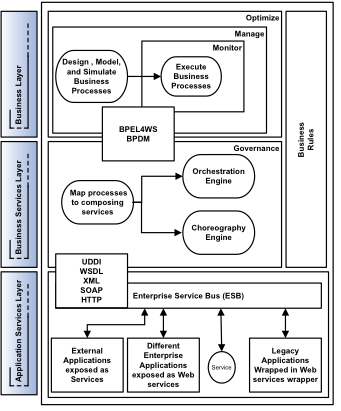
\includegraphics[scale=1, max size={\textwidth}{\textheight}]{BS2}
\caption{Proposed \gls{SOA} and \gls{BPMS} alignment model}
online: http://zoom.it/hIWB
\label{BS2}
\end{center}
\end{figure}

Business layer enables business executives to handle business processes as information, \gls{BPMS} resides in this layer. Business services layer is the layer that maps \gls{BPM} concepts and requirements addressed by \gls{BPMS} into \gls{SOA} based IT infrastructure and \gls{EIS}s. \index{Enterprise Information System} Application Services layer holds the core services ready to be consumed by different BPMSs and shared among enterprises.

\subsection{Business Layer}
Business layer is responsible for supporting business process life cycle. Business process lifecycle consists of five stages: design, model, simulate, monitor, manage, and optimize business processes. Business layer users are either business analysts, or business managers \cite{BS60}. Business analysts create the initial drafts of the business processes, and business managers will manage and monitor those business processes.
Business Process Modeling Notation (\gls{BPMN}) is the standard developed by Business Process Management Initiative (BPMI) to provide a notation that is readily understandable by all business layer users. Utilizing UML to model business processes were presented in \cite{BS61, BS62, BS63, BS64}. \gls{BPMN} provides a number of advantages to modeling business processes over the UML; it offers a more conductive process flow modeling technique, and a solid mathematical foundation to map to business execution languages, whereas UML is not. \gls{BPMN} can map to UML \cite{BS65}. \gls{BPMN} has been intended as a human readable layer that hides the complexity of designing business processes in executable \gls{XML} languages.

Business rules describe the enterprise’s constraints, policies, and rules that apply to in achieving its goals. Business contracts are the constraints, policies, and rules orientation among enterprises. Agile enterprises need to present business rules repositories that can be managed, maintained, and checked against current or new executing business processes and / or services.

For business layer to achieve required functionality, a suitable IT architecture should be presented. IT architecture that utilizes Web services in order to obtain Web services advantages within organizations is presented at the Application Services layer. The connection between business layer and application layer is presented at Business Services Layer.

\subsection{Business Services Layer}
Business services layer holds orchestration and choreography engines under governance mechanisms to map business processes to composing Web services. Orchestration and choreography engines are the mapping enablers of business processes into executable services. Web services are stateless services that can not maintain business logic, operation flow, or user state; so, the need of an orchestration layer to include business logic is addressed. Orchestration and choreography engines maintain business process workflow logic, performance requirements, and system/user state. Business services layer has access to business rules repository.

\gls{BPMN} maps to \gls{BPEL4WS} in order to translate designed business processes into executable orchestration and choreography Web services actions \cite{BS65}. \gls{BPMN} maps to \gls{BPEL} either directly or via \gls{XPDL}. \gls{XPDL} is a format standardized by the Workflow Management Coalition (\gls{WfMC}) to interchange Business Process definitions among different BPMSs. The goal of \gls{XPDL} is to store and exchange the process diagram, to allow one tool to model a process diagram, and another to read the diagram and edit, another to "run" the process model on an \gls{XPDL}-compliant \gls{BPM} engine. \gls{XPDL} is not an executable programming language, but specifically a process design format that literally represents the "drawing" of the process definition. \gls{XPDL} is effectively the serialization of \gls{BPMN}, as well as any non-\gls{BPMN} design method or process model which use in their underlying definition the \gls{XPDL} meta-model. \gls{XPDL} maps to \gls{BPEL4WS}.

\gls{BPEL4WS} allows \gls{BPMS} to transform business processes into executable complex processes by creating and wiring together different activities that can perform Web services invocations, manipulate data, throw faults, or terminate a process. These activities may be nested within structured activities that define how they may be run, such as in sequence, or in parallel, or depending on certain conditions [66]. \gls{BPEL} is an "execution language" designed to provide a definition of Web services orchestration, specifically the underlying sequence of interactions, and flow of data from point-to-point. For this reason, \gls{BPEL} is best suited for straight-through processing or data-flow application integration. New \gls{BPEL} extensions that include BPEL4People and \gls{BPEL} Extension for Sub Processes (BPEL-SPE) are proposed.

A new specification that is expected to be adopted in 2007 is the Business Process Definition Metamodel (BPDM). BPDM is an \gls{XML}-based proposal developed by the Object Management Group (OMG) that will define a set of abstract business process definition elements for specification of executable business processes that execute within an enterprise, and may collaborate between otherwise-independent business processes executing in different business units or enterprises." The specification developed in response to this RFP is expected to achieve, among other things:
\begin{itemize}
\item The ability to integrate process models for workflow management processes, automated business processes, and collaborations between business units.
\item Support for the specification of Web services choreography, describing the collaboration between participating entities and the ability to reconcile the choreography with supporting internal business processes.
\end{itemize}
Governance refers to putting a consistent process in place to make sure there are checks and balances that ensure that the expected results happen. In the case of \gls{SOA}, governance refers to keeping checks and balances between business and IT, between the business and government regulations, and between service and performance \cite{M38}. Governance rules are maintained explicitly in the proposed model to be checked by executing orchestration and governance engines to present flexibility for executing engines and ease manageability of applied rules. The separation of orchestration and choreography engines from business processes and composing services increased enterprise agility because the workflow logic encapsulated by an orchestration and choreography engines can be modified or extended in a central location \cite{BS58}.

\subsection{Application Services Layer}
Application services layer holds applications exposed as services, newly added services, and legacy applications wrapped by standard Web services interface. Services at Application Services layer are set of stateless Web services that perform certain task(s). Business process is the summation of tasks performed by one or more services of application services layer at the sequence maintained by orchestration and choreography engines. Services of Application Services layer are reusable among different business processes, can be integrated in new applications, and can be extended address new business processes.
Legacy systems are computer systems that have been in operation for a long time, and whose functions are too essential to be disrupted by upgrading or integration with another system despite its poor competitiveness. Legacy systems compatibility with modern equivalents has been facilitated via wrapper services. Wrapper service is a type of integration service that encapsulates and exposes logic residing within a legacy system via standard Web services interface to be integrated in the new \gls{SOA} based systems. Utilizing \gls{SOA} for building new applications within enterprises exposes the ease of integration capabilities between new adapted/developed applications and existing applications.
In \gls{SOA}, messages are critical to delivering end-to-end services. Messages must be guaranteed a quick and correct delivery. To enhance messages transportation between services, \gls{SOA} can use an enterprise service bus (ESB). ESB is the Infrastructure software that makes reusable business services widely available to users, applications, business processes, and other services [67]. ESB is a special layer that runs on top of the network that provides a guaranteed messaging service for the most important messages on the network, including the messages that the components of \gls{SOA} continuously exchange. Adopting ESB in \gls{SOA} solutions is not a must, but a recommended best practice.


\section{SOA Selected Topics}
\subsection{Business Stackholders and SOA}
Companies that need customizable solutions or use IT for competitive value, companies seeking to leverage IT capabilities for business advantage, these are companies that should care about \gls{SOA}. Business stakeholders should care about \gls{SOA} adoption if a business wants to be more responsive to their markets, increase market share, and improve customer loyalty, anything that represents a business outcome where IT can make a difference. Many of these benefits cannot be realized without a synergistic relationship between business and IT, which requires that stakeholders in business and IT understand enough about \gls{SOA} to help make its promised benefits a reality. Although IT has a larger role in \gls{SOA} adoption, active business participation will be necessary to achieve strategic goals and ensuing \gls{SOA} benefits. Reasons include, not only:
\begin{itemize}
\item Pursuing business or IT transformation initiatives
\item Seeking faster time to value from IT
\item Transforming or modernizing strategic applications
\item Attempting to lower the lifetime cost of applications or infrastructure
\item Pursuing reuse as a goal to bring products or capabilities to the market faster
\item Looking for greater flexibility in strategic applications
\item Increasing revenue
\item Reducing business process cycles
\item Reducing time and costs for systems integration
\end{itemize}
\subsection{SOA ROI}
Early \gls{SOA} adopters have not focused on measuring \gls{ROI} for \gls{SOA} because bigger, more-profound forces are impacting decisions:
\begin{itemize}
\item how to change the ratio of IT spend so that more is spent on innovation rather than costs
\item how to make strategic applications more flexible
\item how to deliver faster value to the business
\item how to be more responsive to their customers and markets
\item and how to improve business performance.
\end{itemize}
Without \gls{SOA} the long-term cost of the IT solution to the business will be higher. There are several reasons for non-\gls{SOA} solutions having a higher cost, with the most prevalent being that non-\gls{SOA}s don’t have flexibility built in. \gls{SOA} reduces the lifetime cost of an IT solution, and this is a key \gls{ROI} metric. Several studies by vendors, analyst firms, and third parties consistently show that when asked, surveyed, or evaluated, 100\% of clients who have successful \gls{SOA} adoptions report and show improved flexibility, another key ROI metric.
\subsection{Measuring SOA Effectiveness}
Measuring the effectiveness of \gls{SOA} starts with identifying specific value propositions and assigning a suitable metric for assessing and tracking. When looking at effectiveness, the following value propositions are viable and potential metrics:
\begin{itemize}
\item \textbf{Improve IT’s ability to respond to the businesses needs:} Metrics: Reduced calendar time to deploy new solutions, increase in types of changes business stakeholders (non-IT) can make, opportunity value related to faster time to market
\item \textbf{Speed up delivery time:} Metrics: Reduced hours or \% of development schedule, reduced test cycles or time
\item \textbf{Improve flexibility of applications}: Metrics: \% reduction in life cycle time from concept to production, elapsed days a functional type changes (e.g., regulatory rules) can be deployed into production, number of changes that business users can make or deploy, speed of moving through test environments
\item \textbf{Improve flexibility of business processes}: Metrics: Number of processes that can be reconfigured, number of services being used, number of standard business processes.
\end{itemize}
Measuring the efficiency of \gls{SOA} also begins with identifying value propositions and assigning metrics. Efficiency measurements, like effectiveness metrics, require organizations to baseline data so that improvements can be measured and tracked. Common efficiency value propositions include the following:
\begin{itemize}
\item \textbf{Reduce the lifetime cost of applications}: Metrics: Reduction in resources for maintaining code; reduction in cost for fixing code-related problems in production; reduction in number of defects, number of services being created, number of services being created with a single consumer
\item \textbf{Reduce cost of integration}: Metrics: Number of application using shared \gls{SOA} infrastructure, integration cost avoided or reduced by production- deployed infrastructure, reduced cost of building interfaces and infrastructure to support application integration
\item \textbf{Improve productivity}: Metrics: Person days required to build a service, cost to build a service, project delivery times are shortening, number of projects being delivered, improvements in time to market for new capabilities
\item \textbf{Reuse of \gls{SOA} assets}: Metrics: Number of services with multiple consumers, number of services being consumed, service reuse ratios
\item \textbf{Support long-term sunset strategy for applications}: Metrics: Number of common functions from multiple applications converted to services
\end{itemize}
\subsection{SOA Governance Effectiveness}
For most organizations, when there is a failure to achieve any of the following, a red flag should be raised as to the effectiveness of \gls{SOA} governance:
\begin{itemize}
\item Reduce the time to deploy business functions or changes to existing functions
\item Reuse \gls{SOA} assets by other projects or lines of business
\item Improve flexibility of applications
\item Utilize ESB to reduce costs
\item Reduce maintenance costs
\item Achieve development savings in new development of shared services
\end{itemize}
\subsection{Design and Run time SOA Governance}
Design time governance includes the definition of policies and proper life cycle associated with a service as it is designed, tested, implemented, monitored, and registered in the service registry. Design-time governance provides a full life cycle view of a service from inception to deployment to retirement. Design-time governance uses registry and repository tools to track service design, management, policies, and any artifacts associated with the service. Such artifacts might include a test report demonstrating that a service successfully passed certain quality-assurance tests. Design-time governance includes design tools to facilitate the modeling and creation of services, deployment tools addressing service implementation, and test tools. Runtime governance uses the operational policies to monitor the runtime execution of the services against the policy criteria defined and against operational requirements such as service level agreements. Runtime governance practices address managing the quality of a service such that a service is known in the context of its application flow or business transactions. 

\section{Summary}
Business Agility is a relatively new paradigm painted as a solution for maintaining competitive advantage during times of uncertainty and turbulence in the business environment. Business agility consists of three interoperable components: Human, Business Process, and Technical agility. Human are the initiators and maintainers of enterprises agility. Business Process agility can be maintained by applying \gls{BPM} concepts. \gls{BPM} concepts are achieved via \gls{BPMS}. Technical agility has gained new perspectives by adapting \gls{SOA} for \gls{EIS}s. \index{Enterprise Information System} \gls{SOA} based applications are being heralded as the only viable way to overcome the complexities involved in supporting agile enterprises. Business agility principles are satisfied via utilizing \gls{SOA} for \gls{BPMS} by providing the capability of:
\begin{itemize}
\item Translating enterprise mission and practices into information that can be communicated and interpreted. This translation is addressed by presenting the business rules as an external standalone repository that reflects enterprises constraints, policies, and practices. Business rules guides interactivity relations among enterprises.   
\item Replacing traditional \gls{EIS} with adapted one with specific governance mechanism. Governance mechanisms are exploited explicitly in the presented over executable service via orchestration and governance engines.
\item Providing dimensions for each business process that manage its relationship with other different enterprise entities. Business processes are presented in the model as new information type that has an external repository and management, and monitoring activities.
\item Implementing business process lifecycle on different levels. Business process lifecycle is one of \gls{BPM} promises about business process processing. Business process lifecycle phases include: model, design, simulate, execute, monitor, and optimization.
\end{itemize}

\section{Review Questions}
\begin{enumerate}
\item What is Business Agility?
\item What are Business Agility Principles?
\item Define each of the following:
\begin{enumerate}
\item \gls{TQM}
\item \gls{BPR}
\item \gls{WfMS}
\item \gls{BPM}
\item \gls{BPMS}
\end{enumerate}
\item How can we measure SOA effectiveness?
\item How can we measure SOA governance effectiveness?
\end{enumerate}

\section{Exercises and Labs}
In Labs, you shall be getting familiar with Java programming language, as it is the programming language we will be using to build, deploy, and consume different online Webservices and \gls{SOA} systems presented in this book.


\chapter{Integrating UMIS and LMS}
e-Learning is the "learning" process revolution enabled by new technologies that, hopefully, will present an effective and efficient learning process that doesn't exist today. \gls{LMS}s are responsible for "learning" activities, while university management information systems (\gls{UMIS}s) are responsible for handling University managerial activities.
Sociotechnical systems recognized many years ago that organizations functioned most effectively when their social and technological networks were compatible \cite{UMIS55}. This is the case exactly with e-Learning systems. \gls{LMS}s can't provide the managerial functions needed to support universities, and \gls{UMIS}s don't support the "learning" process. Both systems have to integrate and operate together to support educational institutions and e-Learning.

In my attempt to clarify this confusion, I thought about surveying a prototypical e-Learning model and presenting one of the \gls{UMIS} models, casting them side-by-side to help clarify the confusion by highlighting their differences. My goal is to make this piece of research available to students and e-Learning researchers, so we can together overcome this confusion and start focusing on the "learning" process as the main asset of "e-Learning."

\section{Introduction}
When you type "e-Learning" into a search engine, you find the word has been widely used to refer to computer-based systems that do not necessarily maintain the objective of "learning."

Researchers believe that one of the goals of introducing e-Learning was to revolutionize the learning process, either by facilitating many of the challenges that face instructors and learners daily, or by presenting opportunities that might have not existed before.

Evaluating e-Learning is a wide and tough research field that needs more work. Some e-Learning researchers believe that utilizing technology within the learning process has not to date achieved many objectives because requirements were not addressed correctly and clearly. Too often, the learning process and its main activities were neglected for the sake of introducing and focusing only on the technological aspects. The same group believes that one road to a solution is to start by addressing effective future e-Learning requirements, current e-Learning shortcomings, and today's technological limitations. Others, such as the University of Phoenix believe that online learning has achieved quite a bit of success and diffusion.

\section{Learning Models}
e-Learning can be thought of as the learning process created by interaction with digitally delivered content, services, and support \cite{UMIS10, UMIS14, MNAS05}. It involves intensive use of information and communication technology to serve, facilitate, and revolutionize the learning process \cite{EV02, R02, R01, R03, UMIS52}.

Figure \ref{Ms1} presented in page \pageref{Ms1} shows three main learning models that we have come to recognize over the years \cite{EV02, R02, R03, UMIS52}.
\begin{figure}
\begin{center}
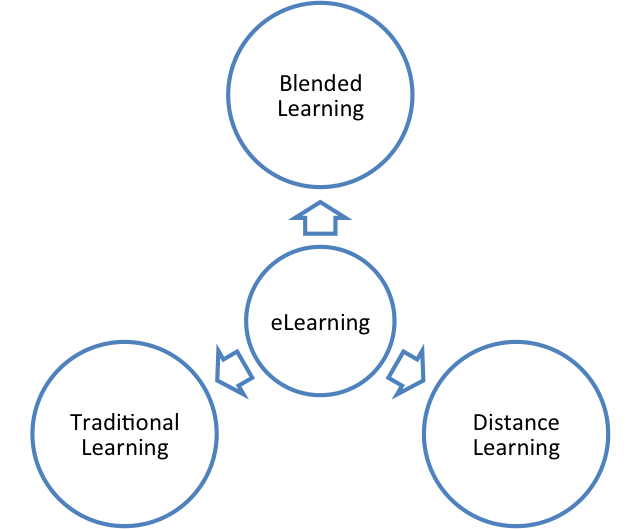
\includegraphics[scale=1, max size={\textwidth}{\textheight}]{Ms1}
\end{center}\caption{Learning Models}
\label{Ms1}
\end{figure}

\begin{enumerate}
\item \textbf{Traditional learning:} In traditional learning, students head to a school, college, or other physical space in which to learn. Information and communication technology can enhance the learning process, but is not necessarily included. For example, data show and presentations can be thought of as an implementation of e-Learning within a traditional learning institution [26].
\item \textbf{Distance learning} In distance learning, an instructor and students are separated by time, location, or both. Education or training courses are delivered to remote locations via synchronous or asynchronous means of instruction \cite{UMIS11}. Distance education does not preclude the use of the traditional classroom \cite{UMIS32}.
\item \textbf{Blended learning} Blended learning combines multiple models to learning. For example, students in a traditional class can be assigned both print-based and online materials \cite{UMIS52}.
\end{enumerate}

\section{UMIS}
e-Learning tends to revolutionize and manage the learning process \cite{UMIS04}, not only to manage universities. Ignoring the learning process while designing and developing e-Learning systems leads to \gls{MIS}, which are important in managing educational institutions activities and help educational institutions achieve a mature level of automation, but are not themselves learning-focused systems.

Managing universities activities requires a university management information system. \gls{UMIS} refers broadly to a computer-based system "collection of hardware, software, people, data, and information" that provides managers with the tools for organizing, evaluating, and efficiently running their departments \cite{UMIS33, UMIS54}.

Examples of \gls{UMIS} components include a student information system (SIS), a library information system, a faculty information system, and a finance system, as illustrated in Figure \ref{Ms2} presented in page \pageref{Ms2}. Below, I present each component in brief detail, listing the reasons they can't be considered part of an e-Learning system.
\begin{figure}
\begin{center}
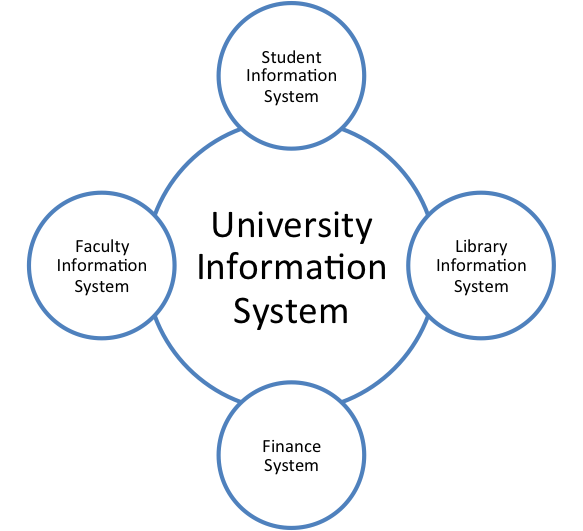
\includegraphics[scale=1, max size={\textwidth}{\textheight}]{Ms2}
\end{center}\caption{Prototypical University Management Information System}
\label{Ms2}
\end{figure}

\subsection{Student IS} 
Student Information System (SIS) is the \gls{IS} responsible for managing students' data at the university. A typical student record in the SIS might includes the student's ID, social security number, name, age, gender, address, email, username, password, date of birth, faculty, university status, and department \cite{UMIS47}.

SIS by itself is not an e-Learning system because personal data that it provides and manages differs in nature than data required for education \cite{EV01}. For example, the SIS should not be able to provide things like detailed records of what the student has already learned (at the level of learning object, rather than a module or program), or a profile of his or her learning preferences, or a development portfolio of transferable skills. On the other hand, a learning portfolio might actually include a history of the student's interaction with tutors, peers, and other significant learning conversations.

This kind of data is intended to be used to force the learning process to be a learner-oriented by adapting the system to fit the learner's needs, characteristics, and capabilities. Unfortunately, SIS does not serve this purpose, and does not handle such data \footnote{The informative model is the model that forces one way of information transformation from instructor to learner, no matter what the personal differences are, whereas the learner-oriented model modifies the system to fit the individual based on personal data.}.

\subsection{Library IS}
Library information systems are responsible for managing and automating libraries within faculties and/or universities. Automated libraries contain material in digitized form \cite{UMIS39}. The \gls{DB} records in these libraries reflect the managerial tasks performed by librarians in order to effectively manage the libraries. A typical record will include ISBN, name, authors, keywords, and data like section, a list of all books, a list of available books, a list of borrowed books, who is borrowing, when the books are due to return, and so forth.

Automated library information systems do not in and of themselves serve the learning process and thus are not on their own considering e-Learning systems. Learners should be able to access fully available digital libraries as part of the learning process.

\subsection{Faculty IS}
Faculty information systems manage and automate managerial activities related to instructors, employees, courses, and the intersections between them. A typical faculty information system \gls{DB} record includes 1) faculty data: ID, name, departments, courses data; 2) course information: course id, name, description, instructors; and 3) faculty personal data: ID, social security number, name, age, gender, address, email, username, password, date of birth, year, department; and 4) employee data, which is the same as the instructor's data but with customized data about one's job \cite{UMIS47}.

A faculty information system's main goal is to organize faculty and university managerial activities; the learning process is not part of the main objective and therefore it is not, on its own, considered e-Learning. The system's capabilities are to generate courses reports, for example, that includes course managerial issues.

\subsection{Finance System}
A finance system manages financial issues related to any organization, even if this organization is a faculty or university. However, I believe financial issues of the educational institution doesn't have anything to do with e-Learning at all. Though e-Learning systems might encompass some financial issues of selling courses, that doesn't entitle the e-Learning system to include a complete set of a university's financial system.

\subsection{UMIS Role}
\gls{UMIS} achieved success over the years and proved efficiency and effectiveness within educational institutions. \gls{UMIS} is required for any successful e-Learning implementation in the three learning models, but with constraints about the role it should play. \gls{UMIS} manages educational institutions, and more attention should be paid to the learning process with the presence of \gls{UMIS} \cite{UMIS31}.

\section{Prototypical e-Learning}
Researchers have tried to define a prototypical e-Learning system over the years, resulting in different points of views, not to mention a variety of terms acronyms. Each term reflects its presenter's point of view and what system features must be present. Some of these terms are:
\begin{itemize}
\item adaptive teaching system \cite{UMIS41}
\item assessment management system \cite{UMIS50}
\item authoring system \cite{UMIS03}
\item CAI: computer assisted instruction \cite{UMIS21, UMIS24}
\item CAPA: computer assisted personalized approach \cite{UMIS51}
\item CBT: computer-based training
\item CIT: computer-information-television \cite{UMIS44}
\item collaborative learning \cite{UMIS20}
\item computer managed learning system \cite{UMIS07}
\item computer assisted learning \cite{UMIS07}
\item \gls{CMS} \cite{UMIS34}
\item courseware authoring tool \cite{UMIS02}
\item distance education \cite{UMIS09, UMIS23}
\item electronic courses \cite{UMIS28}
\item enterprise \gls{CMS} \cite{UMIS30}
\item online courses \cite{UMIS28}
\item integrated student information system \cite{UMIS56}
\item LCMS: learning content management systems \cite{UMIS53}
\item \gls{LMS}: \gls{LMS}
\item interactive learning environment \cite{UMIS17}
\item integrated learning system \cite{UMIS08}
\item PLE: personal learning environment
\item telecast \cite{UMIS27}
\item virtual college \cite{UMIS28}
\item virtual conference \cite{UMIS01}
\item virtual classroom \cite{UMIS19}
\item virtual university \cite{UMIS37}
\item VLE: virtual learning environment \cite{EV01}
\item WBT: web based training \cite{UMIS53}
\item web-based interactive course \cite{UMIS25}
\end{itemize}
By studying all these terms, it's clear that there is some confusion regarding which tools, features, and concepts each includes in its definition. In attempt to organize those acronyms, extract features, and tools, clarify concepts—and keeping in mind that the learning process is the main concern—Figure \ref{Ms3} presented in page \pageref{Ms3} shows one way to categorize them together.
\begin{figure}
\begin{center}
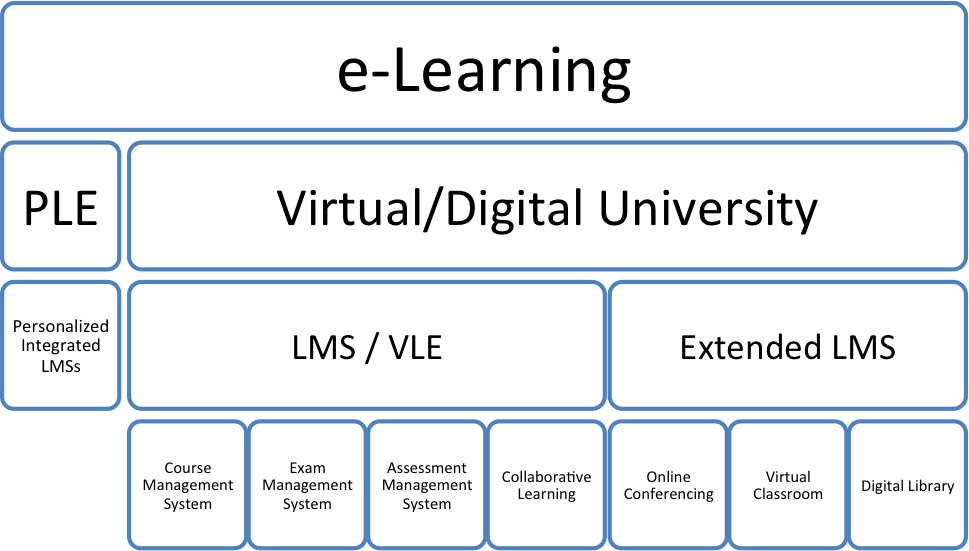
\includegraphics[scale=.8, max size={\textwidth}{\textheight}]{Ms3}
\end{center}\caption{As an umbrella term, "e-Learning" covers many features.}
\label{Ms3}
\end{figure}
e-Learning implements technology that enables virtual/digital university, and/or personal learning environments. A virtual or digital university is a university that implements online \gls{LMS}s or \gls{VLE}s and provides tools for virtual college. e-Learning is the main concept that includes enabler technologies implementation for both virtual/digital university and personal learning environments (PLE). [\gls{LMS} and \gls{VLE} reflect the same implementation of the same concept. \gls{LMS} is widely used in the U.S. and was presented in 1980, while \gls{VLE} is used in U.K. and was presented in 1983 \cite{UMIS09}.]

PLE represents a new trend in e-Learning that claims student's right to use only one gateway to be able to access different \gls{LMS}s provided by different universities. Those different \gls{LMS}s should be personalized and integrated within this gateway and be able to interchange educational student data and information, so provide students with portability between different systems.

Universities and colleges are digitized by implementing ICT. The maximum extent of digital university is the virtual university, where the whole learning process is managed and maintained digitally. \gls{LMS}, \gls{VLE}, and extended \gls{LMS} are the main implementation of e-Learning today.

\section{LMS and VLE}
\gls{LMS} and \gls{VLE} are more or less interchangeable, and \gls{LMS} is used to refer to both. \gls{LMS} is the software that automates the administration of training. The \gls{LMS} registers users, tracks courses in a catalog, records data from learners, and provides reports to management.

An \gls{LMS} is typically designed to handle courses by multiple publishers and providers. It usually doesn't include its own authoring capabilities. Instead, it focuses on managing courses created by a variety of other sources \cite{UMIS10, UMIS14}. Britain and Liber give an example of atypical \gls{LMS} \cite{EV01}.

\gls{LMS} features can be categorized into four main separate systems as depicted in Figure \ref{Ms4} presented in page \pageref{Ms4}. Those four systems are concerned with courses, exams, assessments, and collaborative features. \gls{LMS} can be thought of as the integration of four separate systems, each presenting specific functionalities via specific tools. Figure \ref{Ms5} presented in page \pageref{Ms5} depicts the most common features that should be available in each of those four separate systems.
\begin{figure}
\begin{center}
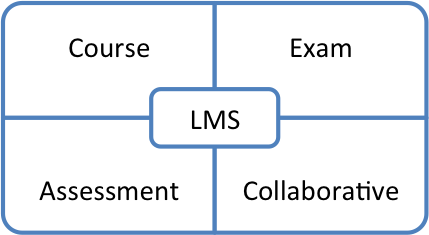
\includegraphics[scale=1, max size={\textwidth}{\textheight}]{Ms4}
\end{center}\caption{The Main \gls{LMS} Functionalities}
\label{Ms4}
\end{figure}

\begin{figure}
\begin{center}
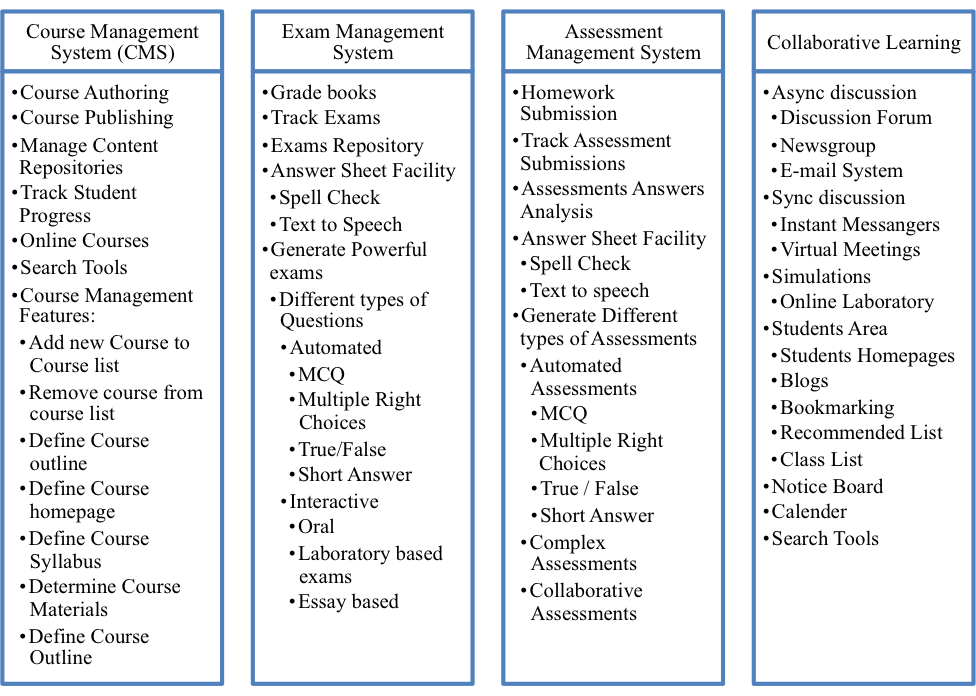
\includegraphics[scale=1, angle=90, max size={\textwidth}{\textheight}]{Ms5}
\end{center}\caption{\gls{LMS}s offer a long list of component functionality.}
\label{Ms5}
\end{figure}

\subsection{Extended LMS}
Extended \gls{LMS}s include added functionality that doesn't necessarily provide e-Learning per se, such as communication tools and digital libraries. Communication tools, such as support for online conferencing and chat, enable or enhances communication among instructors and students and support the existence of a virtual community.

\subsubsection{Online conferencing}
Providing conference capabilities over the internet is known as online conferencing, and it can be take three different forms:
\begin{enumerate}
\item Data conferencing \cite{UMIS43}, or sharing data interactively among several users in different locations. Data conferencing is made up of virtual whiteboards and application-sharing software, which are often used in conjunction with an audio or video connection. A whiteboard is the electronic equivalent of a chalkboard or flip chart, and participants at different locations can simultaneously write and draw on an on-screen notepad visible to all the participants. Application-sharing software is the same as remote control software, in which multiple participants can interactively work in an application that is loaded on only one user's machine. Application "viewing" is similar to application "sharing" except that only one person can manipulate what's visible.
\item Audio conferencing usually takes place when there are three or more people who are geographically dispersed. It is provided by a conference function in a multi-line telephone, or by the telephone companies in some countries, or via VOIP \cite{UMIS42}.
\item Video conferencing is a real-time video session between two or more users or between two or more locations. Videoconferencing may comprise any number of end points \cite{UMIS44}.
\end{enumerate}
\subsubsection{Virtual Classroom}
A virtual classroom is the online learning space where students and instructors interact \cite{UMIS32}. Virtual classrooms provide unique online features \cite{UMIS16} such as:
\begin{itemize}
\item chat
\item discussion: chat between more than two participants, which can be made public or private
\item question and answer: individual participants may ask questions, and instructors may provide public or private answers
\item whiteboard
\item group browser: displaying the same screen to a geographically dispersed group
\item break-out sessions, which allow a subset of learners to use a private chat area within the virtual classroom.
\end{itemize}
\subsubsection{Digital Library}
Digital libraries are libraries that contain electronic materials \cite{UMIS39}. Digital libraries' implementations might include digital data from academic institutions, public libraries, government agencies, and museums \cite{UMIS40}.

Digital libraries play an important role in the learning process due to the tremendous amount of data available to any of the \gls{LMS} components anytime, and anywhere. My faculty is working currently on a project to digitize graduation projects or final works as a main source of information to fresh students and as a mean to communicate back and forth between instructors and students. This digital library will be available online so readers can review books authored by faculty instructors (if they approve, of course), and review graduation projects ideas, concepts, and documentation. Hopefully this project will enhance students' graduation projects by giving them a digital library of their colleges' work, and enhancing knowledge-sharing and collaboration among faculty.

\section{UMIS OR LMS}
Universities require both \gls{UMIS} and \gls{LMS} for efficiency and effectiveness. Neither \gls{UMIS} nor \gls{LMS} can replace the other. University managerial requirements are addressed by \gls{UMIS}, and learning process requirements are addressed by \gls{LMS}. Universities need both!

Open-source \gls{LMS}s are ones for which the source code is available. Free \gls{LMS}s can be downloaded and offer unlimited use, but do not typically provide source code. Commercial \gls{LMS}s are another option and typically come with tech support. By surveying \gls{LMS}s, it is clear to find that most \gls{LMS}s implement same features as depicted in prototypical \gls{LMS}s as the one depicted in "Supporting Education and Research—A higher education committee"(from Joint Information Systems Committee). Table \ref{MsT1} lists the most important Open Source, Commercial, and Free \gls{LMS}s.

\begin{table}
\begin{center}
\caption{Examples of Currently Available \gls{LMS}s}
\begin{tabularx}{\textwidth}{|X|X|X|}
\hline Open-Source	& Commercial & Free \\
\hline .LRN & BlackBoard & KnowEdge eLearning Suite \\
\hline COSE & Desire2Learn & \\
\hline LON-CAPA & IntaLearn & \\
\hline moodle & WebMentor & \\
\hline ATutor & Janison Toolbox & \\
\hline Claroline & Unicon Academus & \\
\hline Eledge & BSCW & \\
\hline KEWL & Colloquia & \\
\hline ILIAS &  eCollege AU+ & \\
\hline MimerDesk & Internet Campus Solution & \\
\hline SAKAI & IBM Lotus & \\
\hline OLAT & Centra & \\
\hline  & The Learning Manager & \\
\hline  & Angel & \\
\hline
\end{tabularx}
\end{center}
\label{MsT1}
\end{table}

One of the international initiatives that provides information to learning institutions on investing in and using information technology infrastructure is e-Framework for Education and Research. Its primary goal is to facilitate technical interoperability within and across education and research communities through improved strategic planning and implementation.

e-Framework's techniques are not intended to be applied immediately; rather, the initiative promotes a journey that takes steps and stages to achieve interoperability goals.

Socio-technical systems recognized many years ago that organizations functioned most effectively when their social and technological networks were compatible. \gls{LMS}s are responsible for learning activities while \gls{UMIS}s are responsible for handling University managerial activities.

But both \gls{UMIS}s and \gls{LMS}s have to integrate and operate together to support educational institutions and e-Learning.

\section{IBM Lotus}
IBM Lotus is one of the leading \gls{LMS}s that implements too many complicated features at a high level [81,82]. IBM Lotus is one of \gls{LMS} dominants [83]. Figure \ref{Ms6} presented in page \pageref{Ms6} presents a detailed Lotus architecture and list of functions that are performed by Lotus components.
IBM Lotus is AICC certified since 1997 [82]. By studying Lotus preview [84] and architecture [85], it becomes clear that it is not applicable to satisfy all the educational institutions requirements within one \gls{LMS} no matter what efforts are attempted by companies. Concerning Lotus as one of \gls{LMS} leaders, neither the presence of 11 servers nor letting down some of the functionalities is acceptable. Issues like scalability, interoperability, and integration have been mainly serious issues for current available commercial \gls{LMS}s that forced many educational institutions towards in-house \gls{LMS} development and implementation to satisfy educational institutions special requirements.
\begin{figure}
\begin{center}
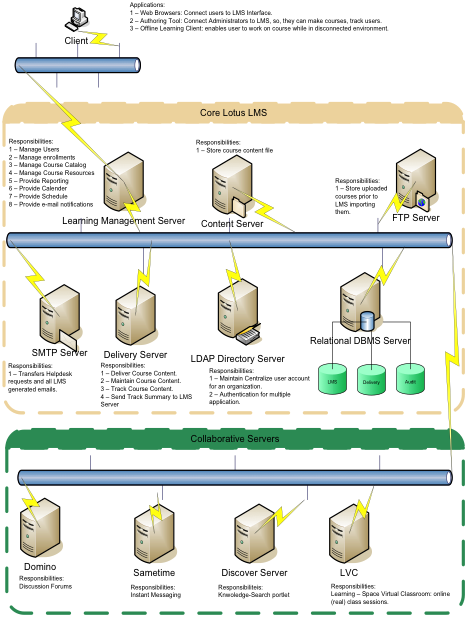
\includegraphics[scale=.9, max size={\textwidth}{\textheight}]{Ms6}
\caption{Detailed IBM Lotus Architecture}
online: http://zoom.it/TYkM
\end{center}
\label{Ms6}
\end{figure}

\section{Evaluation of Current LMSs}
Research is an academic activity that comprises defining and refining the problems, formulating hypothesis or suggested solutions, collecting, organizing, and evaluating data, making deductions and reaching conclusions, and at last carefully testing the conclusions to determine whether they fit the formulating hypothesis [86]. Evaluation is a main step of scientific research that enables in concluding and reporting research results, efficiency, effectiveness, and goals achievement. Evaluation utilizes many of the same methodologies used in traditional scientific and social research, but because evaluation takes place within a political and organizational context, it requires group skills, management ability, political dexterity, sensitivity to multiple stakeholders and other skills that scientific and social research in general does not rely on as much [87]. Evaluation-is the collection and analysis of information by various methodological strategies to determine the relevance, progress, efficiency, effectiveness, and impact of programs activities [88, 89, 90]. Evaluating \gls{LMS} is not like evaluating any software system, because \gls{LMS} should address pedagogical aspects, beside architectural and managerial aspects as depicted in figure \ref{Ms7} presented in page \pageref{Ms7}. 
\begin{figure}
\begin{center}
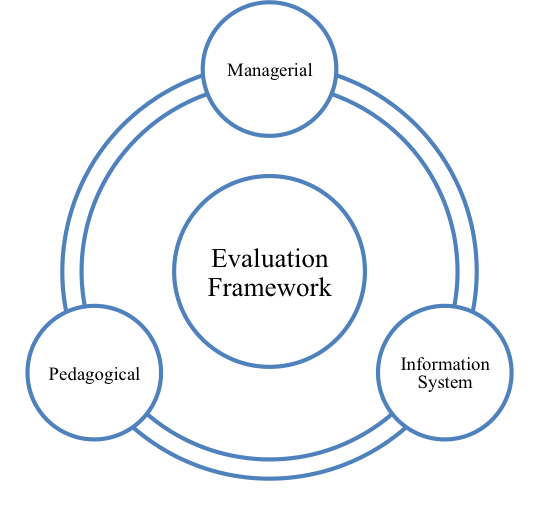
\includegraphics[scale=.9, max size={\textwidth}{\textheight}]{Ms7}
\end{center}\caption{\gls{LMS} Evaluation Framework}
\label{Ms7}
\end{figure}

\subsection{Managerial Evaluation}
Total Cost of Ownership (TCO), among other methodologies like Cost-Benefit Analysis (CBA), is widely used as an analytical and justification tool for software assessment, replacement, and acquisition projects. Unfortunately, TCO analysis is time-consuming to complete based on assumptions, and sometimes hard to quantify. TCO evaluation of a Financial Information Systems is available in [91]. Same TCO managerial evaluation model can be applied from the managerial perspective to \gls{LMS}. Managerial \gls{LMS} Evaluation is out of scope.
\subsection{Pedagogical Evaluation}
Pedagogically, \gls{LMS} shall enable universities and educational institutions to provide educational services in an easy, effective, and efficient manner. \gls{LMS} providers and evaluators must be aware of pedagogical effects that will affect instructors and students. Current \gls{LMS}s do not provide the required pedagogical effects \cite{UMIS07}. One of the reasons is technology limitations. If technologies applied in \gls{LMS} will not enhance learning process then pedagogically it is not a necessity and unfortunately this is the case today.
\subsection{IS Evaluation}
One of the most important models to be used in evaluating \gls{IS}s is the one presented by the standard ISO-IEC 9126. Figure \ref{Ms8} presented in page \pageref{Ms8} presents other architectural parameters that can be used in evaluating \gls{IS}. Presented parameters has not been addressed by ISO-IEC 9126 Standard, but still can be used by \gls{IS}s evaluators. It is evaluators’ responsibilities to determine the most valuable architectural aspects to be considered in the evaluation process. Another architectural evaluation model that deserves mention and well consideration is the one presented in [92].

\begin{figure}
\begin{center}
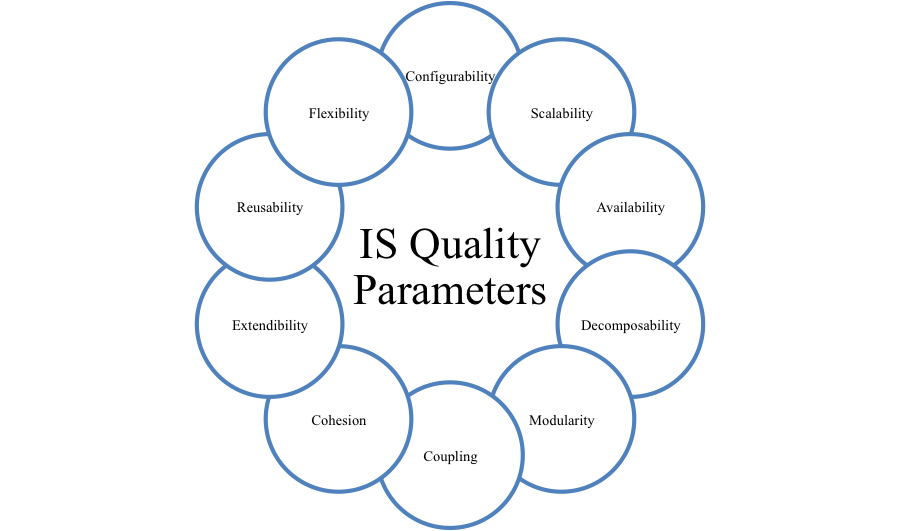
\includegraphics[scale=.9, max size={\textwidth}{\textheight}]{Ms8}
\end{center}\caption{Non-ISO Addressed IS Quality Parameters}
\label{Ms8}
\end{figure}

The study of most well known \gls{LMS}s; including Lotus, has lead to the realization of the reality that there are many shortages of current \gls{LMS}s affecting e-Learning in educational institutions This part tends to present some of the shortages addressed through evaluations of current \gls{LMS}s. Some of the addressed deficiencies are: Integration, Agility, Scalability, Extensibility, Flexibility, Interoperability, and Redundancy.
\subsubsection{Integration}
e-Learning solutions are clearly a combination of two main categories of applications: \gls{LMS} and \gls{UMIS}. As presented in figure \ref{Ms9} presented in page \pageref{Ms9}, there are four integration challenges:
\begin{figure}
\begin{center}
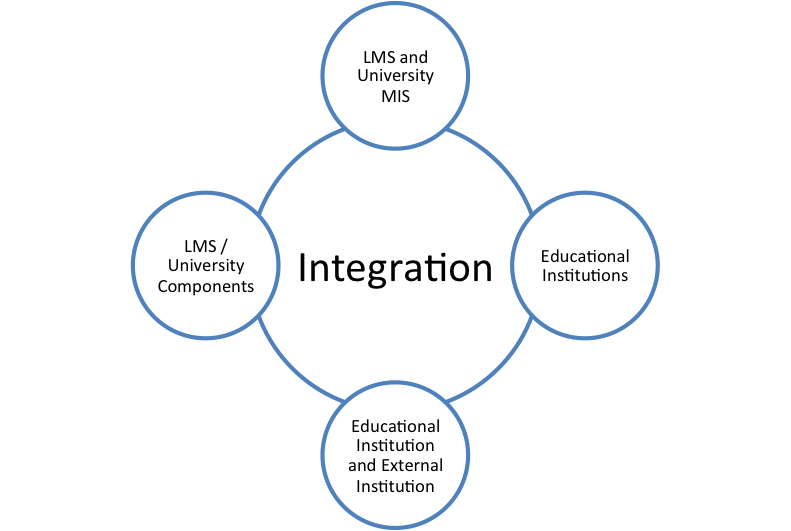
\includegraphics[scale=.9, max size={\textwidth}{\textheight}]{Ms9}
\end{center}\caption{University Integration Challenges}
\label{Ms9}
\end{figure}
\begin{enumerate}
\item \textbf{Category components integration:} Composing applications might come from different software vendors, legacy applications that have been running for a long time needs to be integrated with new applications, and new software applications might be installed. Existing applications might stand in the way of installing new applications due to integration problems.
\item \textbf{\gls{UMIS} and \gls{LMS} integration:} \gls{UMIS} advances \gls{LMS}s by decades \cite{UMIS19}. \gls{UMIS} achieved stability levels that most major educational institutions are running the same \gls{UMIS} for almost a decade with no noticeable problems. \gls{LMS} is the new concept that needs to be added to educational institutions, and it has to integrate with long time running \gls{UMIS}. Due to differences in nature of design objectives between \gls{UMIS} and \gls{LMS}, integration issue should be addressed clearly. There will be new features that university will be able to provide incase full integration of \gls{UMIS} and \gls{LMS} took place. The capability of presenting individualized assessments that can be generated by integrating SIS; which will include two profiles for student; a managerial profile, and an educational profile; and the assessment management system should be addressed. 
The capability of presenting individualized learning plans by integrating \gls{CMS} and SIS that holds the learning profile should be addressed. Personalized courses will be generated based on learner history profile. It is not acceptable by learning experts to fix time and change amount to be learned, instead, amount to be learned should be fixed and personalized. Such individualizations enable PLE.
\item \textbf{Integrate different \gls{LMS}s:} It is hard to find an educational institution that implements only one \gls{LMS} because educational institutions requirements are hardly met by one \gls{LMS} \cite{UMIS07}. Different \gls{LMS}s, either within the same educational institutions or over different ones needs to be integrated. Integration over courses level as provided by utilizing SCORM and AICC is not the typical solution of integration problems, because educational institutions need to share more than courses.
\item \textbf{Integrate educational institution and external institutions:} Educational institutions are not isolated islands that work alone, but they are part of the society. Educational institutions need to be integrated with all other governmental institutions. Tasks like generating a report with all current certain grade students, or students that are qualified for certain task because they have attended certain courses should be easily executed. Querying the educational institutions databases should be available efficiently. Student’s data shall be available to give the student ability to transfer his data between educational institutions as required.
\end{enumerate}

\subsubsection{Agility}
From certain perspective, educational institutions are organizations, just like any other organizations. Organizations need agility, and so do educational intuitions. Agility is the ability to sense change and opportunity, respond quickly, and execute successfully. Educational institutions need to reflect governmental new or modified rules on current \gls{UMIS}, overcome merge and acquisitions challenges, and provide new and customized services based on new added system features. An example of new customized services that should be presented when new system features are added is collaborative assignment. Collaborative assignment can be provided by the system after installing new collaborative tools. If the system were not built with agility in mind, new features adding or existing features editing becomes almost impossible, limiting the system from adapting and presenting new functionalities.

\subsubsection{Scalability}
System should expand and contract its resource pool easily to accommodate to heavier loads. Client – Server based \gls{LMS}s can not scale to support large number of components, or interactions among components, within an active configuration [92]. Most today’s \gls{LMS}s are Client – Server based \cite{UMIS41}. Scalability needs to be addressed to offer educational institutions with the \gls{LMS} solutions that satisfy the increasing requirements.

\subsubsection{Extensibility}
Extensibility is the ability to add functionality to a system. Dynamic extensibility implies that functionality can be added to a deployed system without impacting the rest of the system [92]. That implies not only adding new features to existing \gls{LMS} without the need to install the new version, but also adding customized functionalities required by the educational institution. Unfortunately, current \gls{LMS}s are released periodically to provide new functionality, with the need to install the new version every time. Besides, most commercial \gls{LMS} are categorized according to functions available by each product level, without guarantee on what are exactly the actions required to be taken to make the move to the next level incase required.

\subsubsection{Flexibility}
Flexibility is the ability of a system to respond to potential internal or external changes affecting its value delivery, in a timely and cost effective manner. The ability to change or to be changed according to circumstances is not by default provided by Client – Server architectural based \gls{LMS}s, and unfortunately most \gls{LMS}s are Client – Server based \cite{UMIS41}. Changes include addition/loss of servers, and types of services provided by the system.

\subsubsection{Interoperability}
Interoperability is the capability to communicate, execute programs, or transfer data among various functional units in a manner that requires the user to have little or no knowledge of the unique characteristics of those units [93]. Interoperability is concerned with processes require the system to communicate with external systems to accomplish tasks. Educational institutions need to interact with external systems to achieve tasks successfully. Interoperability between \gls{LMS} and external systems needs to be addressed and enabled. Current commercial \gls{LMS} architectures and used protocols are not provided with \gls{LMS}. A standard interface to \gls{LMS} functionality is required.

\subsubsection{Redundancy}
Redundancy refers to the unmanaged, uncontrolled, and unwanted more than single time occurrences of either data or functionality.

\paragraph{Data Redundancy} refers to existence of the same piece of data in more than one place. Data is said to be in consistent state when all data redundancy are controlled. Data redundancy should be controlled for insert, update, and delete queries. Figure \ref{Ms10} presented in page \pageref{Ms10} depicts an example of uncontrolled data redundancy that causes inconsistent data and system state. SIS, \gls{CMS}, assessment, exam, and finance information systems need student Data, unfortunately with different formats and different types. Questions like which system should manage this data? Shall every system manage its own data? Shall the system take the risk of having a redundant data? Need to be answered.
\begin{figure}
\begin{center}
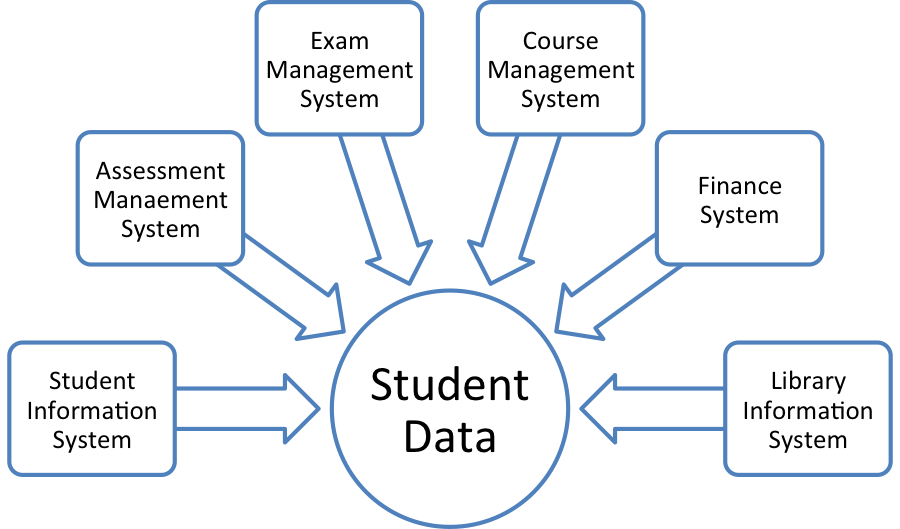
\includegraphics[scale=1, max size={\textwidth}{\textheight}]{Ms10}
\end{center}\caption{Redundant Student Data}
\label{Ms10}
\end{figure}
\paragraph{Functionality Redundancy}: Functionality overlapping and redundancy is clear from the literature review. Functionality redundancy comes from the attempt of \gls{LMS} software vendors to increase the tasks performed by \gls{LMS} to include functions that are not part of it. Redundancy is accepted only if it is managed. 

\section{Selected Topics}
\subsection{SOA and Service Modeling}
Because \gls{SOA} projects vary in size and scope, not all \gls{SOA} projects require service modeling. \gls{SOA} projects whose goals include engineering business applications that are built to change, leveraging and reusing business services, reducing the lifetime costs of an application, or using \gls{SOA} to accelerate time to value require the identification, specification, and realization of services. These \gls{SOA} projects require service modeling. Service modeling produces a categorized list of services, business functionality, and capabilities required by the business. This list can be described as a service portfolio.
\subsection{Applications and Composite Services}
Composite services are not applications but services that invoke other services. The invocation is independent and without knowledge by the consumer that other services are being invoked.
\subsection{BPM and Applications}
\gls{BPM} is a management discipline focused on the following:
\begin{itemize}
\item Aligning business process performance and the results with strategic objectives and business goals
\item Understanding and documenting business processes so that they may be consistently executed
\item Measuring, monitoring, and controlling process performance, including key inputs and outputs
\item Actively designing and improving business processes to meet or exceed the expectations of customers while achieving business goals (e.g., cost and revenue)
\end{itemize}
\gls{BPM} solutions vary from a focus on human-centric business processes, to document and content-focus processes, to structure and system-oriented processes. A business process can be represented as collaboration between components.

\section{Summary}
This chapter presented the \gls{IS}s utilized by educational institutions. They are \gls{UMIS} and \gls{LMS}. \gls{UMIS} serve educational institutions to automate managerial tasks, and \gls{LMS} provides the required functionalities to automate the learning process. Educational institutions need both \gls{UMIS} and \gls{LMS} to satisfy e-Learning and enhance the learning process. Both \gls{UMIS} and \gls{LMS} are composed of collection of task specific applications. Educational institutions; and as a result the learning process, can be enhanced by enhancing the \gls{IS} that serves them. Shortages of current \gls{LMS} are evaluated in order to find solutions that serve educational institutions to better address information, learning, and functionality requirements.
\gls{SOA} (\gls{SOA}) is one of the software architectures that satisfy most of the non-functional requirements addressed by \gls{IS}s. \gls{SOA} principles need to be presented and studied in order to utilize \gls{SOA} for \gls{UMIS} and \gls{LMS} to overcome current \gls{LMS} shortages, limitations, and deficiencies. \gls{SOA} as a design pattern is expected to solve many of the current \gls{IS} problems by easing integration, interoperability, and agility.
The idea of this thesis is to adopt \gls{SOA} in e-Learning via presenting \gls{UMIS} and \gls{LMS} based on \gls{SOA}, and evaluate the proposed components to determine the efficiency of \gls{SOA}. Evaluating \gls{LMS} is not limited by evaluating the architectural style of the system, it shall be expanded to include pedagogical and managerial aspects too.

\section{Review Questions}
\begin{enumerate}
\item What are the main components of \gls{UMIS}?
\item What is the difference between \gls{LMS} and \gls{VLE}?
\item What is Extended \gls{LMS}?
\item What are the perspectives of evaluating \gls{LMS}?
\end{enumerate}

\section{Exercises and Labs}
In Labs, you shall be getting familiar with Java programming language, as it is the programming language we will be using to build, deploy, and consume different online Webservices and \gls{SOA} systems presented in this book.

\chapter{LMS from Monolithic to Services}
\label{LMSFromMonolothicToServices}
\section{Introduction}
e-Learning can be thought of as the learning process created by interaction with digitally delivered content, services, and support. e-Learning involves intensive usage of Information and Communication Technology (ICT) to serve, facilitate, and revolutionize learning process \cite{R01, R02, R03}. Learning methods include traditional learning “face-to-face”, distance learning “complete asynchronous time and place learning delivery; mainly online”, and blended learning “learning that combines instruction lead learning with online learning activities leading to reduced classroom contact hours”. Blended learning has the potential to increase student learning while lowering attend rates compared to equivalent fully online courses \cite{R04}. Blended learning is the learning paradigm that attempts to optimize both traditional learning and distance learning advantages, potentials, and benefits while eliminating both learning paradigms shortages and challenges. Nowadays blended learning is commonly referred to as e-Learning. When compared to traditional learning paradigm, blended learning is found to be consistent with the values of traditional learning paradigm adopted in almost all higher education learning institutions for decades, and has the proven potential to enhance both the effectiveness and efficiency of meaningful learning experiences \cite{R05}.

\gls{LMS} (\gls{LMS}) is the software that automates the administration of education. \gls{LMS} registers students, tracks courses in a catalogue, records data from learners, and provides reports to management. \gls{LMS} is typically designed to handle courses by multiple publishers and providers. It usually doesn’t include its own authoring capabilities; instead it focuses on managing courses created by a variety of other learning resources. Sandy Britain and Oleg Liber present a prototypical \gls{LMS} in \cite{EV01}. Because learning models can be classified into traditional, distance, and blended learning paradigms; universities and educational institutions can also be classified into three classes that map to each learning paradigm. However, nowadays technology and the great advancement in recent Web 2.0 and informal learning methods allowed the existence of completed education programs and courses to be presented online. So, university model can be either Online University “full distance learning model”, Campus University “the one that supports either the traditional or blended learning paradigm”. Campus Universities used to have managerial aspects that can’t be neglected and need to be addressed to enable universities to achieve their goals effectively. University Management Information Systems (\gls{UMIS}) is the software \gls{IS} responsible for managing universities. \gls{UMIS} advances \gls{LMS} with decades. \gls{UMIS} has achieved mature level of well formed business and performance requirements adoption, and usage. Unlike \gls{LMS}; which is the newly introduced \gls{IS} to universities when compared to \gls{UMIS}. \gls{UMIS} and \gls{LMS} needs to be integrated to enable universities present effective and efficient learning.

Architecture is about providing balance in the face of conflicting concerns. Software entities, architectures, have gotten more complex as we have progressed from monolithic to client/server to network-centric architectures and now to \gls{SOA}. Architectural evolution continues to move toward agility and hence the attention and interest in \gls{SOA}. At the heart of every new shift in architecture sits a practically or theoretically compelling concept that brings the paradigm forward. Client/server introduced the distributed application architecture that portioned workloads between service providers and service consumers referred to as clients. Network-centric architectures introduced the Internet as a paradigm shift. Now with \gls{SOA}, services are the architectural game changer, moving the architecture to greater agility.

\section{Problem Definition}
Current Blended Learning Model Paradigm faces many challenges. Those challenges are mainly pedagogical. No one can deny that today’s technologies advances by decades technologies used in teaching and education less than decade ago. However, a number of recent articles have commented that science education is no better today than it was fifty years ago. \gls{NAEP} shows that in most areas today’s students are achieving at about the same levels as students tested in 1971 \cite{R07}. e-Learning researchers know very well that this problem is not caused by technology; because as mentioned before technology has advanced greatly. This pedagogical issue is the result of:
\begin{itemize}
\item The attempt to use whatever technology currently available or becomes available in the near future without pedagogically considering student or the learning process.
\item Allowing technology to stand against the learning process, because no matter what advancement we have achieved, technology is still limiting our dreams (because we still dream about things that we can’t yet achieve technologically), and this situation takes place with e-Learning nowadays.
\item The poor evaluation that is available for many of the innovations. Most of the required evaluations are either inadequate or doesn’t exist at all.
\end{itemize}
Alfred Bork et al. argue that some of the reasons why technology has not led to improvements in learning globally are \cite{R07}:
\begin{itemize}
\item Grabbing Onto Each New Technology: The belief that each new technology will enhance learning needs more arguments about efficiency than just belief.
\item Failure to Continue Successful Development: funders often prefer to look for something new rather than follow up on successful approaches because they want to make a mark by being in the forefront. Funders want to make a statement, and following up on someone else’s work doesn’t provide them with the credit or “name” they desire.
\end{itemize}
Pedagogically, most training methods and technologies produce, at best, “trained novices”. That is, they introduce facts and concepts to students, present them with relatively simple questions to test this new knowledge, and provide them with a few opportunities to practice using this knowledge in exercise or scenarios. However, becoming proficient requires extensive proactive solving realistically complex problems in wide range situations, combined with coaching and feedback from managers, more experienced peers, or other types of experts \cite{R08}.
Most evaluations of today’s presented technologies in the learning model focus on technology aspects of the solution while ignoring the pedagogical aspect; almost at all. The result of using technology, particularly computers, in learning has so far not been impressive. A variety of studies and opinions have questioned the use of technology to improve learning. Although it has been many years since computers have begun to be used in learning environments, there is little improvement in learning, with or without technology. Although the use of technology in learning shows no significant difference, that is, computer learning is no better than traditional instruction, learners have been provided with the convenience of any time, any place learning. Students’ understand and retention improves when students learn by experience. Technologies such as collaboration, interactivity, modelling, simulations, virtual reality interfaces, and gaming will help students experience the skill being taught, but they have not helped students that far yet \cite{R07}. Besides, students lack of awareness of different e-Learning technologies stand up against the presentation of effective e-Learning model.

We started coding in objects after procedural programming and structured design had evolved. Object-oriented programming gave way to the need to design using objects, and then a plethora of object-oriented analysis and design methods and techniques ensued: Rumbaugh, Jacobson, Coad, Wirfs-Brock, and others. Eventually, patterns evolved that took smaller units of programming and built micro architectures that were dubbed design patterns. One of the programming notions that developed into a best practice in object orientation was “program to interfaces, not to implementations.” This separation of concerns allowed greater underlying flexibility in development: both at design time (classification and class associations) and runtime (polymorphism).
With the evolution of objects came the need to group them into larger-grained entities and to build larger-grained components. Component-based development, and later component-based design, created larger structures that were more closely mapped to business intent and needs. When Web services—with the promise of looser coupling and greater standardization than the Common Object Request Broker Architecture (CORBA) or \gls{DCE} came to the forefront and promised to make distributed computing more accessible, programmers started to build remote procedure calls with \gls{XML}-based objects. As the momentum grew, Web services architecture gave way to \gls{SOA}.

\section{Proposed Solution}
Adaptive learning for students with many different backgrounds, learning styles, and interest is almost a must. Educational psychologists by and large agree that students differ greatly in the ways they learn and very few teachers or professors can adapt learning to each student in the typical large classes, the costs associated with delivering different instruction for varied learning styles is prohibitive \cite{R07}. Benjamin Bloom (1984) showed twenty-five years ago, as reported in his 2 sigma paper, that almost all students can learn to the mastery level, given the right learning environment \cite{R09}. In Bloom’s experiments, the most successful learning strategy was tutoring. Adaptive e-Learning that is supported with intelligent techniques and methods is one of the ways to support personalized e-Learning, and so authors believe that it will be the way to solve many of the limitations and today’s e-Learning challenges. Authors will review the different adaptive and intelligent e-Learning systems proposed over a long e-Learning research era, highlighting the maturity of adaptive and intelligent features and the e-Learning researchers attempt to introduce services based e-Learning systems in order to overcome many of the e-Learning challenges, like reusability, scalability, integration, and interoperability. Finally, authors will conclude with the need to present a new learning model that attempts to use the best of what was presented before, and avoid all the challenges and mistakes. Though authors believe there’s no single unified learning model can be the only right model, hopefully this work will be a step towards a better learning model supported with the appropriate technologies.

\section{Adaptive e-Learning Systems}
Computer-based learning systems are criticized by many researchers for their limited ranges and adaptability of teaching actions compared to rich tactics and strategies employed by human expert teachers \cite{R10}. Many universities in the developing countries, started to adopt e-Learning by modifying their network infrastructure, establishing new labs, providing internet connection, and purchasing different tools for creating e-Learning courses and using different \gls{LMS}s. However, these modifications and supplement were not enough to ensure successful e-Learning outcomes because other important elements for e-Learning success were missing such as flexibility of the system, adaptability towards students needs, reusability of learning objects, interoperability between different \gls{LMS}s, effective and official design of e-content \cite{R11}.
Adaptive e-Learning systems would be a good solution for better e-Learning. The absolute majority of Web-enhanced courses rely on \gls{LMS} because they are powerful integrated systems that support a number of teachers and students needs. Though \gls{LMS}s look surprising, indeed for every function that a typical \gls{LMS} perform there is an Adaptive Web Based Educational System (AWBES) that can do it much better \cite{R12}. Adaptivity is the ability to modify e-Learning lessons using different parameters and a set of predefined rules. Researchers differentiate slightly between adaptivity and adaptability by thinking about adaptability as the possibility for learners to personalize an e-Learning lesson by themselves. These two approaches go from machine centred (adaptivity) to learner centred (adaptability). In practice, it is quiet difficult to isolate one from the other due to their close relationship \cite{R13,R14}. Adaptive e-Learning is often meant to be new or in an early development stage \cite{R10}. Christian Gutl defines adaptive e-Learning systems as an environment of software modules, which comprises a set of features for adaptivity and adaptability \cite{R15}. Important factors for adapting to student needs and desires include \cite{R07}:
\begin{itemize}
\item Each Student Should Move at a Unique Pace: Given all the variations between student backgrounds, interests, and abilities, it is highly desirable to allow each student move at a unique pace in the learning units.
\item Adaptation Should be Very Frequent: Changes based on occasional exams are inadequate. Learning activities should adapt to each student on a moment-by-moment basis. Students should feel that the adaptive program is responding to them as individuals. 
\item Each Student Should Be Successful in Learning: a major advantage of adaptive variable placing is that the students can continue to learn in a given area until they have learned the material. We know from Bloom’s research that almost all learners can succeed and achieve mastery, but some learners need more time and more practice than others.
\item When Something Is Successfully Learned, the Learner Should Move On: Often in classroom learning, after a student has learned something, the class continues working on the topic, boring the student. This will not occur in a fully adaptive learning environment.
\item No One Should Be Taught Something S/he Already knows: By assuring learner competencies, avoiding unneeded instruction, and moving each student forward when ready, we expect to achieve a major reduction of learning time, but this cannot be verified empirically until we have a full range of computer-based adaptive learning units.
\end{itemize}
The provision of static learning material will not meet the requirements of the users. Adaptive 
e-Learning enables personalizing learning process to individual learners via adapting some parameters; like identifying, analyzing and monitoring relevant aspects of instructions, such as different velocities, paths, or strategies of learning can be personalized. Performance improvements within the learning process can be gained via adaptive e-Learning systems \cite{R15}. Adaptation and personalization will improve the learning process, therefore, a paradigm shift from the consumption of static learning contents to well tailor and highly personalized learning sessions is needed.
\subsection{Adaptive e-Learning Approaches}
Four main approaches which are used to give a historical overview of adaptive e-Learning can be identified \cite{R10}:
\begin{itemize}
\item Macro-Adaptive Approach: Addresses adaptation of instructions on a macro-level by allowing different alternatives in selecting a few main components such as learning objectives, levels of detail, delivery system, etc. In this approach, instructional alternatives are selected mostly on basis of the student’s learning goals, general abilities, and achievement levels in the curriculum structure. 
\item Aptitude-Treatment Interaction (ATI) Approach: This approach treats adaptation of instructional strategies to specific student’s characteristics. This strategy proposes different types of instructions or even different media types for different students. The most important classes of learner characteristics can be summarized with the following ones: intellectual abilities, cognitive styles, learning styles, prior knowledge, anxiety, achievement motivation, and self-efficiency. One aspect of the ATI approach is the user’s control over the learning process according to the abilities of the students by giving them full or partial control over the style of the instruction or the way through the course. Level of control can be one of three levels: complete independence, partial control within a given task scenario, and fixed tasks with control of pace.
\item Micro-Adaptive Approach: Addresses adaptation of instructions on a micro-level by diagnosing the student’s specific learning needs during instruction and providing instructional prescriptions for these needs.  Researchers have attempted to establish micro-adaptive instructional models using on-task rather than pre-task 
measures.  Monitoring the user’s behaviour and performance, such as response errors, 
response latencies, emotional states, etc. can be used for optimizing instructional treatments and sequences on a very refined scale \cite{R15}. 
\item Constructivistic-Collaborative Approach: Follows the constructivist pedagogical approach. An important element of this approach is the usage of collaborative technologies which are considered often on essential component of e-Learning.  Adaptive system enables learning by focusing on how knowledge is learned and should consider the context, learning activities, cognitive structures of the content, and the time extension. Some new adaptive e-Learning systems take account of students’ motivational factors combining the instructional plan with a “motivational” plan.
\end{itemize}
Over the last decades, various types of adaptation systems and possible areas for their applicability have been identified, thus leading to the emergence of specialized research fields, like \gls{AEHS}, Computer Aided Instruction (CAI), Computer Managed Instruction (CMI), Recommender Systems, \gls{ITS}, Personalized Systems of Instruction (PSI), and many others. Adaptive multimedia systems as an improved learning environment is well documented in the research work of Christian Gutl et al. \cite{R15}.

\subsection{AEHS Overview}
Brusiolvsky thinks about Adaptive Hypermedia Systems as systems that refer to all hypertext and hypermedia systems which reflect some features of the user in the user model and apply this model to adapt various visible aspects of the system to the user. In other words, the system should satisfy three criteria: it should be a hypertext or hypermedia system; it should have a user model; it should be able to adapt the hypermedia using this model \cite{R14}.
\subsubsection{Application Areas of AEHS}
Educational Hypermedia Systems are the most popular area for adaptive hypermedia research,  hence come the term \gls{AEHS} (\gls{AEHS}) and incorporates applications like:
\begin{itemize}
\item Adaptive Textbooks: Adaptive Textbooks use history-based, knowledge-based and prerequisite-based adaptive annotation of links to suggest to the individual user an appropriate path through a learning space by adapting the navigation links \cite{R16}. Adaptive textbooks can help students learn faster and better \cite{R12}.
\item Adaptive Quizzes: Quizzes and Tests are assembled by the system from a pool of questions using student and domain models that are manipulated with automated reasoning machines. Such forms of evaluation are adaptive in a per-question basis. Also it would be desirable to have the questions themselves be adaptive \cite{R17}.
\item Adaptive Class Monitoring: Class Monitoring tools are important to give the teacher much better chances to notice the students lagging behind \cite{R12}. Adaptive Teaching Systems can help instructors adapt lectures and educational contents to fit students.
\item Adaptive Collaboration Support: Intended to capture adaptive support in learning processes that involve communication between multiple persons (and, therefore, social interaction), and potentially, collaboration towards common objectives. Adaptive techniques can be used in this direction to facilitate the communication/collaboration process, ensure a good match between collaborators, and other activities \cite{R18}. Adaptive Collaboration Support can enforce the power of collaborative learning \cite{R12}.
\end{itemize}
\subsubsection{Modeling the User}
Three categories of user related data can be defined and modeled in \gls{AEHS} \cite{R14,R19}:
\begin{itemize}
\item User Data: Refers to information about personal/characteristics of the user. User features that can be stored in \gls{AEHS} include knowledge, goals/tasks, background, hyperspace experience, preferences, interests and individual traits, and cognitive and learning styles.
\item Usage Data: is related to information on the user's interactive behaviour that cannot be resolved to user characteristics. This category include data like: selective actions of the user (clicking on links, scrolling and enlarging operations for hypermedia objects, audio control operations), temporal viewing behaviour rating (users are required to explicitly rate objects, links, WebPages), and purchases and purchase-related actions.
\item Environment Data: comprises aspects of the user environment that are not related to the users themselves. This kind of adaptation has evolved due to Web-based systems. Adaptation decisions may depend on spatial-temporal location of the user, the user platform (such as hardware, software, equipment - computer, PDA, cell phone, digital TV), and network.
\end{itemize}
\subsubsection{Adaptation Taxonomy}
In 1996 Brusilovsky developed a taxonomy providing a way to segment adaptive research into two categories, which was labelled “adaptive presentation and adaptive navigation support” \cite{R20}. Figure \ref{AHT} presented in page \pageref{AHT} shows an updated taxonomy of adaptive hypermedia technologies \cite{R21}. This taxonomy has been illustrated and studied by many researchers \cite{R14,R22}. Whereas the adaptive presentation changes the content presented in the documents, the adaptive navigation support changes the structure of links between the documents and how this navigation structure is presented to the user. 
\begin{figure}
\includegraphics[scale=.8, angle=90, max size={\textwidth}{\textheight}]{AHT*}
\caption{Updated Taxonomy of Adaptive Hypermedia Technologies}
\label{AHT}
\end{figure}

\subsubsection{Adaptive Presentation}
The goal of adaptive presentation is to adapt the content of a hypermedia page to the user’s goals, knowledge and other information stored in the user model. This area concerns the selection and composition of information fragments to be later presented to the user. For example, the system may decide to provide additional explanations as well as to hide content from a novice user, while an expert user in the domain will receive more specific and more detailed information. In a hypermedia system the content of a “page” may not only be text, but it may also contain various items of other media types. The main benefit of the adaptive presentation is that it tries to reduce the amount of presented information to the most relevant information for a particular user, solving the information overload problem of the classic hypermedia systems.
\begin{itemize}
\item Adaptive Multimedia Presentation: the selection of different multimedia fragments (in practice this technique also includes the adaptation of multimedia content, just as the generation of shortened versions, but currently most examples of adaptive multimedia simply select between prefabricated content).
\item Adaptation of Modality: choice among different types of media to present to the user, related to the same content; e.g., for a video we can have full video, still image, text description, or use of them in parallel.
\item Adaptive Text Presentation
\begin{itemize}
\item Natural Language Adaptation: Natural language adaptation cannot be classified further at the moment. Many natural language generation systems do, in fact, make use of fragments (and even paragraphs) of canned text, but distinction here is made between those systems that use natural language technology as a foundation and those that do not. Refinement of this distinction might be needed at a later stage.
\item Canned Text Adaptation: This term includes fragment processing, such as:
\begin{itemize}
\item Inserting / Removing Fragments:  Information related to a concept is broken into several fragments of text (or multimedia content). With each fragment a condition is associated on elements of the user model. When information related to a concept is presented, the system selects only those fragments for which the condition is true. This technique can be used to implement the methods of additional, prerequisite and comparative explanations.
\item Altering Fragments: Can be used for the implementation of the explanation variants method. The \gls{AEHS} stores several variants of the same information fragment, and selects the variant to display based on the user model. For example, each variant is created for different group of users such as beginner, intermediate, and expert.
\item Stretch Text:  Fragments are embedded in a webpage and initially shown or hidden from the user depending on conditions on user model data. \gls{AEHS} can show or hide these fragments also upon explicit user requests. This technique is useful for implementing additional, prerequisite or comparative explanations, but less for explanation variants and not all for sorting.
\item Sorting fragments: This technique is used for the sorting method and presents a set of fragments to the user, ordered from the most relevant to the least relevant according to some criteria based on user’s goal, background, knowledge, etc.
\item Dimming fragments: Used to dim, shade or deemphasize (in some way) a fragment to indicate that it is not (or at least less) relevant for the user.
\end{itemize}
\end{itemize}
\end{itemize}
\subsubsection{Adaptive Navigation Support}
Adaptive Navigation Support modifies or augments the existing set of hyperlinks shown to the user to aid them in finding relevant information with the goal to help users find their way through hyperspace by adapting link presentation and functionality to the goals, knowledge, and other characteristics of an individual user. The goal is to guide the user towards relevant and interesting information and to advise the user not to follow navigation paths that lead to irrelevant information. The main benefit of the adaptive navigation support is that it simplifies the rich link structure and solves the “lost in hyperspace” problem while maintaining the navigation freedom that is typical of hypermedia systems. Adaptive navigation support contains several different techniques that can be used individually or combined to provide navigational support:
\begin{itemize}
\item Direct guidance: \gls{AEHS} outlines visually one of the links on the page showing that this is the best link to follow or generates an additional dynamic link which is connected to the recommended “next” page to visit.
\item Adaptive Link Sorting: \gls{AEHS} uses sorting mechanisms; like ordering links from most relevant to lowest relevant to recommend links to users.
\item Adaptive Link Hiding/Disabling/Removing: \gls{AEHS} tries to prevent the user from following links that are not relevant at the moment. There are several ways to achieve this goal. A link can be hidden by changing the color of the anchors to that of normal text or removing the anchor. Also, link functionality can be disabled and so the link is removed.
\item Adaptive Link Annotation: \gls{AEHS} augments the links with some form of comment, which can tell the user more about relevance of the nodes behind the annotated links. These annotations are usually provided in the form of visual cues such as icons, font colors, sizes, and types.
\item Adaptive Link Generation: \gls{AEHS} may discover new useful links between pages and add them by using previous navigation (by an individual user or a user group) or page similarity to add links.
\item Map Adaptation: This technique consists of a combination of the other techniques, the only difference being that it is applied to a graphical visualization of the navigation structure. The map is usually presented in a separate frame or window.
\end{itemize}

\subsubsection{AIEHS Overview}
Enhancing \gls{AEHS} with methods and techniques from \gls{ITS} creates the \gls{AIEHS}. \gls{ITS} form an advanced generation of Computer-Aided Instruction (CAI) systems with their ability to provide a user-adapted presentation of the teaching material. ITSs have been developed and evaluated for many years in the field of artificial intelligence in education. The emergence of WWW increased the usefulness of such systems. Web-based learning systems should be more intelligent through adoption of artificial intelligence techniques \cite{R01}. Intelligent e-Learning systems include utilizing artificial intelligence techniques, such as decision making, machine learning, planning, scheduling, and cognitive science in e-Learning platforms \cite{R23}. The objective of intelligent e-Learning systems, as is typically conceived, is to provide highly structured lessons that are to a large extent under automated control. Within this framework, the intelligence of the system often appears in the form of adaptive, sequencing or personalization of the course material, adaptive guidance for navigation, or interactive problem solving support. The most interesting opportunities to develop intelligent functionality are related to facilitating collaboration rather than adapting the learning material \cite{R24}. There has never been a clear distinction between intelligent and adaptive e-Learning systems. AI techniques have been widely used to support adaptive e-Learning features. Christopher Paul Bailey presents an agent-based framework to support adaptive hypermedia \cite{R25}.

\subsection{Adaptive e-Learning Applications' Examples}
N. Matar et al. presented what they called “adaptive e-Learning system” to address different adaptive features of e-Learning \cite{R11}. N. Matar et al. argued that the proposed system can help universities; especially newly established ones come over limitations and shortages by presenting a global course repository. Despite the obstacles that can come against such a solution; starting from the required infrastructure and ending with the instructors’ choice to refuse submitting the learning material they have created, centralization as a solution is not the most suitable solution anymore. A. M. Riad and Haitham A. El-Ghareeb argues that shareability among different \gls{LMS}s is the solution to unlock course repositories and presented a \gls{SOA} based \gls{CMS} that integrates different \gls{LMS}s \cite{EV09}. Besides, N. Matar et al. talked about the ‘Unified Adaptive e-Learning System’ as the proper solution to adaptive e-Learning implementation ignoring the fact that adaptive e-Learning solutions doesn’t come in the ‘one solution fits all scenarios’. Adaptive e-Learning solutions differ from different cultures, and different learning scenarios. Instead of attempting to unify adaptive e-Learning, integrating different adaptive e-Learning modules together to establish an adaptive upon request e-Learning solution is the best solution.

\section{Intelligent e-Learning Systems}
Artificial Intelligence (AI) utilizes programming algorithms to simulate thought processes and reasoning that produce behaviour similar to humans. A successful implementation of AI could be tested using a Turing Test approach, in which a human interacts with an interface that could have either a human or computer on the other end. The test is considered successful if the human is unable to determine whether there is a computer or a human on the other end. The applications of AI within e-Learning can produce the potential of creating realistic environments with which students can interact. The student essentially would interact with the \gls{IA}s which in turn perceive changes in the simulated environment. The \gls{IA}s would then communicate perceived changes in the environment back to the student who then makes decisions based upon their own perceptions of the environment \cite{R27}. 
Current learning technologies can help create trained novices more efficiently, but they are really not up to the job of creating true experts. For example, multimedia Computer Based Training (CBT) systems are good at presenting information and then testing factual recall using multiple choice or fill-in-the blank questions. However, traditional CBT systems are incapable of providing intelligent, individualized coaching, performance assessment, and feedback students need to acquire broad and deep expertise \cite{R08}.
Employing the state-of-the-art artificial intelligence (AI) technology in current e-Learning systems can bring personalized, adaptive, and intelligent services to both students and educators. Although we have seen more and more successful applications of AI in e-Learning, most of them have not yet been expanded to or adopted in widely used e-Learning systems, especially open-source \gls{LMS}s (\gls{LMS}) such as \gls{moodle}, Sakai and so on. This observation takes us to the analysis and discussion of the current work in both \gls{LMS} and applied AI. The findings include that current intelligent \gls{LMS} systems are still in their early stage, while AI applications need to handle some problems or to be modified before applying them into the \gls{LMS} systems, and AI technology also needs to be brought to open source communities \cite{R28}.

\subsection{Evolution of AI in e-Learning}
Koschman views the evolution of Computer Based Instruction (CBI) as a series of paradigmatic shifts in the field of Instructional Technology. According to Koschman, the initial CBI paradigm, entitled Computer-Assisted Instruction (CAI) emerged in 1960 with the release of Coursewriter I \cite{R29}. Koschman argues that the next paradigm shift \gls{ITS} was founded by members of the AI community who had migrated to the educational community. Their motivation was as follow:
“Research in AI is founded upon the conjecture that cognition is, in some sense, a computational process than can be studied through the construction of “intelligent” systems that serve as functional models of the otherwise inaccessible processes of the human mind. If machines can be programmed to display intelligent behaviour, there is no reason, at least in principle, that systems could not be designed to assume the role of a skilled teacher. Since one-on-one tutoring is commonly considered the gold standard against which other methods of instruction are measured, the paradigm is founded on the proposition that education could be globally improved by providing every student with a personal (albeit machine-based) tutor” \cite{R29}.

\subsection{AI Methods and Techniques}
AI methods and techniques enable computer programs and software applications to think and act intelligently and rationally. To achieve this goal, AI utilizes methods and techniques, like: Neural Networks, Genetic Algorithms, Reinforcement Learning, and Fuzzy Logic.

\subsubsection{Neural Networks}
Neural Networks do not rely on ruled-based programming for their performance. Instead, neural networks use learning algorithms to “tune” outputs to inputs. The technology finds use in situations in which rules are not explicitly available, and in which “tuning” inputs to outputs is easier than analyzing the internal reasoning process. Currently, \gls{DM} uses neural networks to analyze the large volumes of data \cite{R30}. J.E. Villaverde et al. presents a feed-forward neural network to recognize automatically the learning styles of individual students according to the actions that he or she has performed in an e-Learning environment \cite{R31}.

\subsubsection{Genetic Algorithms}
Genetic Algorithm is the population containing a number of trial solutions each of which is evaluated to yield fitness and a new generation is created from the better of them. The process is continued through a number of generations with the aim that the population should evolve to contain an acceptable solution. Mu-Jung Huang et al. presents an approach to adaptive e-Learning based system that utilizes Computerized Adaptive Testing to identify the learner applicability for a learning topic, and then the Genetic Algorithm and Case-Based Reasoning (CBR) are employed to construct an optimal learning path for each learner. Mu-Jung Huang et al. presented a genetic-based curriculum sequencing approach that will generate a personalized curriculum sequencing \cite{R32}. Anna Hovakimyan et al. presents another Genetic Algorithm based e-Learning system that is based on so called “teaching-scenario” and capable of creating the appropriate sequence of the teaching resources from the set of all possible teaching resources based on quantity and quality \cite{R33}.

\subsubsection{Fuzzy Logic}
Fuzzy set theory provides a formalism in which the conventional binary logic based on choices "yes" and "no" is replaced with a continuum of possibilities that effectively embody the alternative "maybe". Formally, the characteristic function of set X defined by f(x) =1 for all x in X and f(x)=0 for all x not in X is replaced by the membership function. J. Vrettaros et al. presents a fuzzy logic based correction tool that can be utilized in e-Learning systems. Test correction tool utilizes fuzzy logic rules in classifying students based on their answers and rigidity of correction levels \cite{R34}. Y. Chen uses feedback and fuzzy self-organizing map to improve adaptive e-Learning model via continuously updating teaching material by tracking learner grades and achievement level \cite{R35}. K. K. Loo presents genetic algorithm utilization in SmartTutor that can identify the weaknesses of a learner in an e-course and advice the learner how to do revision efficiently \cite{R36}.

\subsubsection{SW Agents as AI Implementation}
Software Agent is a program that performs some information gathering or processing task in the background. Typically, an agent is given a very small and well-defined task \cite{MNAS02}. Software Agent is a physical or virtual entity which:
\begin{itemize}
\item Is capable of acting in an environment.
\item Can communicate directly with other agents. 
\item Is driven by a set of tendencies (in the form of individual objectives or of a satisfaction/survival function which it tries to optimize). 
\item Possesses resources of its own. 
\item Is capable of perceiving its environment (but to a limited extent). 
\item Has only a partial representation of its environment (and perhaps none at all). 
\item Possesses skills and can offer services. 
\item May be able to reproduce itself. 
\item Its behavior tends towards satisfying its objectives, taking account of the resources and skills available to it and depending on its perception, its representation and the communications it receives.
\end{itemize}
\subsubsection{SW Agents Characteristics}
Agents are capable of acting, not just reasoning. Actions affect the environment which, in turn, affects future decisions of agents. The main attributes and characteristics of Software Agents are \cite{MNAS02}:
\begin{itemize}
\item Autonomy: A key property of agents is autonomy. They are, at least to some extent, independent. They are not entirely pre-programmed but can make decisions based on information from their environment or other agents. agents have capabilities of task selection, prioritization, goal-directed behavior, decision-making without human intervention
\item Mobility: Although this property is optional, it certainly characterizes some agent systems. It is interesting to note that in the natural world, agent intelligence is always associated with agent mobility (animals). Other living things (plants) have no intelligence.
\item Persistency: code is not executed on demand but runs continuously and decides for itself when it should perform some activity.
\item Social ability: agents are able to engage other components through some sort of communication and coordination; they may collaborate on a task.
\item Reactivity: agents perceive the context in which they operate and react to it appropriately.
\end{itemize}
An agent is an encapsulated computer system that is situated in some environment and that is capable of flexible, autonomous action in that environment in order to meet its design objectives. Software Agents are \cite{R38}: 
\begin{itemize}
\item Clearly identifiable problem-solving entities with well defined boundaries and interfaces. 
\item Situated (embedded) in a particular environment; they receive inputs related to the state of their environment and they act on the environment through effectors.
\item Designed to fulfill a specific purpose; they have particular objectives (goals) to achieve. 
\item Autonomous; they have control both over their internal state and over their behavior. 
\item Capable of exhibiting flexible problem solving behavior in pursuit of their design objectives; they need to be both reactive (able to respond in timely fashion to changes that occur in their environment) and active (able to act in anticipation of future goals). 
\end{itemize}

\subsubsection{Intelligent SW Agents}
\gls{IA} is a software agent that exhibits some form of artificial intelligence. While the working of software agents used for operator assistance or \gls{DM} (sometimes referred to as bots), are often based on fixed pre-programmed rules, "intelligent" implies the ability to adapt and learn.
\begin{itemize}
\item Ability to Adapt: Adaptation implies sensing the environment and reconfiguring in response. This can be achieved through the choice of alternative problem-solving-rules or algorithms, or through the discovery of problem solving strategies. Adaptation may also include other aspects of an agent's internal construction, such as recruiting processor or storage resources.
\item Ability to Learn: Learning may proceed through trial-and-error, then it implies a capability of introspection and analysis of behavior and success. Alternatively, learning may proceed by example and generalization, then it implies a capacity to abstract and generalize.
\end{itemize}
In some literature IAs are also referred to as “autonomous \gls{IA}s” \cite{R39}, although autonomy is generally assumed for agents. IA systems should exhibit the following characteristics:
\begin{itemize}
\item learn and improve through interaction with the environment (embodiment)
\item adapt online and in real time
\item learn quickly from large amounts of data
\item accommodate new problem solving rules incrementally
\item have memory based exemplar storage and retrieval capacities
\item have parameters to represent short and long term memory, age, forgetting, etc.
\item be able to analyze itself in terms of behavior, error and success
\end{itemize}

\subsubsection{SW Agents Challenges}
When several agents (inter)act they may form a multi-agent system. Characteristically such agents will not have all data or all methods available to achieve an objective (this can be referred to as "limited viewpoint") and thus will have to collaborate with other agents. Also, there may be little or no global control and thus such systems are sometimes referred to as swarm systems. As with distributed agents, data is decentralized and execution is asynchronous. Earlier, related fields include Distributed Artificial Intelligence (DAI) and Distributed Problem Solving (DPS).
Multi-Agent architecture standards were attempted in order to force \gls{MAS} standardization and global integration. Knowledge Query and Manipulation Language (\gls{KQML}) was presented in order to support knowledge sharing among agents \cite{BS50}. Knowledge Interchange Format (\gls{KIF}) is a computer-oriented language for the interchange of knowledge among disparate programs developed by the \gls{ARPA}-sponsored Knowledge Sharing Effort \cite{R41}. The OMG group proposed a reference model as an attempt to standardize the development of agent technologies \cite{R42}. \gls{KAoS} is described as "an open distributed architecture for software agents.'' The \gls{KAoS} architecture describes agent implementations (starting from the notion of a simple generic agent, to role-oriented agents such as mediators and matchmakers), and elaborates on the interactive dynamics of agent-to-agent messaging communication by using conversation policies \cite{R43}. The Foundation for Intelligent Physical Agents (\gls{FIPA}) is a multi-disciplinary IEEE standardizing group pursuing the standardization of agent technology. \gls{FIPA}'s approach to \gls{MAS} development is based on a "minimal framework for the management of agents in an open environment'' \cite{R44}. Unfortunately, as a result for all the standardization effort, there were no universally accepted commercially supported standard yet.

\subsubsection{SW Agents based e-Learning Systems}
Utilizing Software Agents in e-Learning systems have been known to e-Learning researchers very well. Alfredo Garro  and Luigi Palopoli \cite{R45} proposes an \gls{XML} based Multi-Agent System to support Chief Learning Officers in defining roles, associated competencies and knowledge level required; manage the skill map of the organization; measure human resources competence gaps; support employees in filling their competence gaps as related to their roles; enrich a given courseware or create personalized learning paths according to feedbacks user provides in order to optimize the acquisition of needed competencies; and assist Chief Learning Officers in choosing the most appropriate employee for a given role. A strong well presented utilization of Multi Agent Systems in performing different tasks. 
Using software agents as recommenders to students has been presented by O.R. Zaiane \cite{R46}. Zaiane presented a recommender system in an e-Learning context that tries to "intelligently" recommend actions to a learner based on the actions of previous learners. This recommendation could be an on-line activity such as doing an exercise, reading posted messages on a conferencing system, or running an on-line simulation, or could be simply a web resource. The use of web mining techniques to build such an agent that could recommend on-line learning activities or shortcuts in a course web site based on learners' access history to improve course material navigation as well as assist the online learning process was presented. 

\subsubsection{ITS}
In the early 1970s a few researchers defined a new and ambitious goal for computer-based instruction. They adopted the human tutor as their educational model and sought to apply Artificial Intelligence techniques to realize this model in “intelligent” computer-based instruction \cite{R47}.
\gls{ITS} are complex, integrated systems that apply Artificial Intelligence (AI) techniques to problems of education and training. \gls{ITS} uses Artificial Intelligence techniques to customize instructions according to the student’s needs. ITSs strive to optimize learning of domain concepts and problem solving skills by means of adaptive, individualized coached practice on domain tasks \cite{R48}.
The goal of ITSs would be to engage the students in sustained reasoning activity and to interact with the student based on a deep understanding of the students’ behaviour. If such systems realize even half the impact of human tutors, the payoff for society promised to be substantial \cite{R47}. 
The closest computational analogy to an \gls{ITS} is an \gls{ES}, while the closest educational analogy is a Computer-Assisted Instructional (CAI) system \cite{R49}. \gls{ITS} can be thought of as Intelligent Computer Aided Instruction (ICAI).  \gls{ITS} is an educational software containing an artificial intelligence component. The software tracks students' work, tailoring feedback and hints along the way. By collecting information on a particular student's performance, the software can make inferences about strengths and weaknesses, and can suggest additional work.\index{Knowledge Management System}

\subsubsection{ITS Modules}
\gls{ITS} rely on three types of knowledge, organized in three separate software modules namely Domain, Pedagogical, and Student modules as depicted in figure \ref{ITS} presented in page \pageref{ITS} \cite{R08,R48}.
\begin{itemize}
\item Domain Knowledge Base Module: is the set of questions being taught. Represents subject matter expertise and provides the \gls{ITS} with knowledge of what it is teaching. This module let the \gls{ITS} know what it is teaching.
\item Pedagogical Modules: contains the methods of instruction and how the knowledge should be presented to the student, enables \gls{ITS} to know how to teach, by encoding instructional strategies used by the tutoring system. This module lets the \gls{ITS} know how it is teaching.
\item Student Module: Represents the student’s knowledge, skills, and other attributes that affect how the student should be taught. This module lets the \gls{ITS} know who it’s teaching.
\end{itemize}

\begin{figure}
\begin{center}
\includegraphics[scale=.4, max size={\textwidth}{\textheight}]{ITS}
\end{center}\caption{ITS Block Diagram}
\label{ITS}
\end{figure}

\subsubsection{ITS Limitations and Challenges}
A variety of AI techniques are used to capture how a problem can be solved. Major \gls{ITS} systems capture subject matter expertise in rules. Though rules enables \gls{ITS} to generate problems on the fly, combine and apply rules to solve the problems, assess each learner’s understanding by comparing the software’s reasoning with theirs, and demonstrate the software solutions to the participant’s, B. H. Sreenivasa Sarma and B. Ravindran argues that Rule based \gls{ITS} challenges include \cite{R48}:
\begin{itemize}
\item There are many rules which a system can use to teach efficiently, but which are very difficult to encode.
\item It is difficult to incorporate the knowledge that human teachers use, but cannot express. The machine tutors have a different set of data available than the human tutors, so the knowledge that could improve the tutor’s performance is ignored.
\item Rule-based systems are not adaptive to new student’s behavior.
\end{itemize}
While there has been a sustainable research effort in the application of artificial intelligence to education over the past three decades with some notable success stories, intelligent tutoring has had relatively little impact on education and training in the world. There are several reasons for this lack of penetration \cite{R47}:
\begin{itemize}
\item ITSs are expensive to develop and until relatively recently, the necessary computing power was expensive to deploy.
\item Ontogeny of the field and the consequences for software evaluation. The creative vision of intelligent computer tutors has largely arisen among artificial intelligence researchers rather than education specialists
\end{itemize}

\subsubsection{Examples of ITSs}
Edward R. Sykes and Franya Franek present a Web-Based Architecture of an \gls{ITS} for Remote Students Learning to Program Java that is called JITS \cite{R50}. JITS utilizes an Intelligent Module to define errors at student submitted code. Student code is passed to Java Parser; that checks student code for errors. When errors found, a fuzzy logic based semantic engine is used to define error spots and notify students to correct them, and the process takes place till code is verified. Besides, JITS contextually offers students’ help by giving hints about the proper programming method that shall be used (for example: for loop instead of if-then statement). JITS is a Web-based solution that utilizes distributed architectural components. Most ITSs lack evaluation results; and JITS is one of them. Though JITS utilizes Web based architecture, it is always a challenge to integrate Agents based systems with external systems. It is believed that this integration challenge limits the widespread utilization and usage of software agents in real life world scenarios.

\section{SOA in e-Learning Systems}
\gls{SOA} (\gls{SOA}) is a design pattern that presents IT infrastructure and \gls{IS}s architecture as loosely coupled, fine granular services that can address system requirements once they are presented either by adding new services or modifying existing ones. \gls{SOA} also addresses enterprises information systems’ inefficiency by enhancing reusability, thus theoretically, shortening \gls{IS}s development time and effort required. Besides reusability, interoperability and integration are other main driving forces for adopting \gls{SOA} in e-Learning systems. \gls{W3C} defines Service as ‘A Component capable of performing a task’. Service is ‘A vehicle by which a consumer’s need or want is satisfied according to a negotiated contract (implicit or explicit) which includes Service Agreement, Function Offered and so on’. \gls{SOA} is the design pattern that utilizes services concept to achieve architectural advantages. \gls{W3C} defines \gls{SOA} as ‘A set of components which can be invoked, and whose interface descriptions can be published and discovered’. This definition can be expanded to include the science, art and practice of building applications, so \gls{SOA} can be defined as ‘The policies, practices, frameworks that enable application functionality to be provided and consumed as sets of services published at a granularity relevant to the service consumer. Services can be invoked, published and discovered, and are abstracted away from the implementation using a single, standards based form of interface’ \cite{R51}.

\subsection{Webservices as SOA enabler}
Web services are applications that use standard transports, encodings, and protocols to exchange information \cite{R52}. A Web service is a software system designed to support interoperable machine-to-machine interaction over a network. \gls{W3C} defines Web service as “A software system designed to support interoperable machine-to-machine interaction over a network. It has an interface described in a format that machines can process (specifically \gls{WSDL}), Other systems interact with the Web service in a manner prescribed by its description using \gls{SOAP} messages, typically conveyed using \gls{HTTP} with \gls{XML} serialization in conjunction with other Web-related standards” \cite{R53}. Web service can also be defined as ‘A programmatic interface to a capability that is in conformance with Wsnn protocols’. Wsnn protocols are present efforts in the \gls{W3C} and more recently in OASIS to reach a Web service maturity model. Wsnn protocols include \gls{WSDL}, \gls{SOAP}, and \gls{XML} \cite{R54}. \gls{SOAP} is a lightweight protocol intended for exchanging structured information in a decentralized, distributed environment \cite{R55}. \gls{XML} solves a key technology requirement that appears in many places. By offering a standard, flexible and inherently extensible data format, \gls{XML} significantly reduces the burden of deploying the many technologies needed to ensure the success of Web services \cite{R56}. Web services is a general framework that expedites the sharing of heterogeneous data and software resources dispersed on the internet. The standard-based resource sharing and platform-neutral characteristics of Web services have motivated many organizations to apply the technology in diverse areas, such as \gls{SCM}, virtual enterprise, homeland defence, e-government, and e-business \cite{R57}.

\subsection{SOA and e-Learning Systems}
Many researchers have realized the importance of utilizing \gls{SOA} in e-Learning systems. Integration, interoperability, scalability, and reusability are the main axis that \gls{SOA} based e-Learning researchers attempt to address, solve, and enhance e-Learning systems. Though some researchers ignored the pedagogical features of e-Learning systems, others considered those features as the main motivator of adopting \gls{SOA} in e-Learning.
Declan Daggar \cite{R58} argues that e-Learning is moving from passive to active; because the learner is getting more involved with the learning experience. Besides, technology emerging from the adaptive hypermedia, semantic web, mobility and distributed computing communities are being widely employed in online learning, and steps towards Service-Oriented eLearning platforms needs to be taken. Declan Daggar et al. classifies \gls{LMS}s into three generations: First Generation “Monolithic”, Second Generation “Modular”, Third Generation “Service-Oriented”. First generation focused on presenting learning content without tracking learner activities. Second generation enhanced the learning process but cannot stand handling new technologies, interoperability and integration between evolving systems like third generation shall do. Declan Daggar et al. argues that interoperability needs to be on control basis not just on data basis. Service-Oriented \gls{LMS} technologies include adaptive hypermedia and semantic web. Though Service-Oriented \gls{LMS} standards are still evolving, attempts to address service-oriented \gls{LMS}s are many, and include the abovementioned research project, and many other projects like the ones described in the following sections.

\subsubsection{\gls{moodle} and Webservices}
Al-Ajlan and Zedan \cite{R59} presents a research work that focuses on “assignment” modules based on \gls{moodle}  and the steps to enrich it with Web services. Al-Ajlan and Zedan argues that Web services is important and required in integrating different \gls{moodle}(s) resources; especially assignments, and to provide the capability for more than one instructor to be working on the same course. Instructor can search for the best assignment within different \gls{moodle}(s) instances and retrieve it. Al-Ajlan’s proposed work utilizes PHP based \gls{SOAP} Web services to integrate best with \gls{moodle}. There is no evaluation presented at his research, however it presents a good utilization of UML in describing Web services specifications. Though the research work title includes \gls{SOA}, the common misusage of Web services as \gls{SOA} is clear in this research. Though Web services are main \gls{SOA} enabler, \gls{SOA} is not just Web services.

\subsubsection{Services based e-Learning Systems and Reusability}
One of the good utilization of \gls{SOA} in e-Learning is presented by Moon Ting Su et al. \cite{R60} to address the reusability capabilities provided by \gls{SOA}. Moon Ting Su et al. argues that Instead of building an e-Learning system from scratch, it can be assembled by choosing the required functionalities from a set of Web services related to e-Learning. Moon Ting Su et al. study results in a set of Web services for the e-Learning domain. The description for each of the Web services is as follows:
\begin{itemize}
\item Assessment Web service: This service supports the delivery and scoring of assessment. Lecturers are able to create/edit/delete quiz or assignment, quiz or assignment questions using this service. Students on the other hand are able to take the quiz online at specific time and duration defined by the lecturers. The result of objective-type question will be displayed immediately after the students finish the quiz. Students’ answer for subjective question can be retrieved from the server for marking later.
\item Grading Web service: This service supports grading based on the marks. Marks submitted by lecturers will be graded automatically based on the grading scheme uploaded by the administrator of the e-Learning system. Feedback can be submitted together with the grade.
\item Marking Web service: This service provides the automated marking functionalities for multiple choices assessment. For subjective assessment, the marking scheme is defined using rubrics. Rubric is a guide for assessing a piece of student’s work and aids in achieving consistency in marking.
\item Course Management Web service: This service allows lecturers to manage the courses (uploading, editing and deleting of lecture materials). It also allows the users to manage their favourites’ resources. Users can also search, view and download the learning resources. The searching is done based on the Learning Object Metadata (LOM) metadata elements provided by the creator of the learning resources.
\item Metadata Web service: This service is developed based on LOM standard. It allows users to upload the learning objects together with its metadata. The metadata is useful in managing, searching and locating the learning object.
\item Registration Web service: This service allows administrator of an e-Learning System to create new users, edit and delete the existing user profiles and also delete particular users.
\item Reporting Web service: This service generates the performance report for quiz by using Crystal Report.
\end{itemize}
In the abovementioned study, there are different points of strength and excellence. The main functionalities of typical e-Learning systems are built using Web services. The strength of this approach is reusability and interoperability. Developing a new e-Learning system will involve assembling the required Web services. The e-Learning system can be developed and run on different hardware and software platforms. However, the disadvantage of this approach is if the server that hosts the Web services is off-line, the e-Learning system which depends on these Web services will not be operational. Another important feature of this study is the use of rubrics in guiding the instructor to evaluate subjective assessment. Rubrics improve consistency in the evaluation of students’ work especially when there is a large number of student and multiple instructors are involved in the evaluation. Another good point of the proposed research is the commitment to \gls{ELF}  and e-Learning standards as depicted in the architecture presented at the study.
However and to repeat from almost all services based \gls{LMS}s, \gls{SOA} is not Web services. This chapter presents a bunch of Web services that collectively do not form \gls{SOA} in any manner. Our experience in evaluating \gls{SOA} in e-Learning highlighted that problem. Because we started by building services for every component without \gls{SOA} governance and without defining what are the system features that needs to be exposed as services, we found ourselves building the entire system as services from scratch, and it seems this is the case in this research too. Besides, there is no indication of implementation at all, and so evaluation was not mentioned at all. It is really rare to find evaluation for \gls{SOA} based e-Learning systems. May be because \gls{SOA} adoption in e-Learning systems is new to some extent, or may be because it is really too much easier to present frameworks and architectures than it is to implement them.

\subsubsection{Services based e-Learning Systems and Scalability}
Another \gls{SOA} based framework for e-Learning Systems is presented by Chih-Ping Chu et al. \cite{R61}. Chih-Ping Chu et al. addresses the scalability issues of educational institutions and propose a \gls{SOA} based e-Learning framework to address scalability capabilities of \gls{SOA}. This research handles the educational institutions incapability of maintaining large scalable \gls{LMS}s by grouping \gls{LMS}s services (based on \gls{ADL} Seven services as depicted below) into local and global groups. Local services group which constitutes the “Local \gls{LMS}” are provided and maintained internally while other services can be spread over the internet. \gls{ADL}  modularize \gls{LMS} into seven services: Tracking, Delivery, Learner Profile, Course, Sequencing, Content Management, Testing/Assessment. Chih-Ping Chu et al. argues that tracking and delivery services shall compose local \gls{LMS} while rest of the services can be spread globally. Authors argue that maintaining learning material might exhaust educational institution resources, so Local \gls{LMS} will not store learning material, however it will acquire it from different places.
\gls{LMS} is described as a highly generalized model consisting of seven parts that provide the functionality of learner/learning tracking, content delivery, course import/export and content sequencing:

\begin{itemize}
\item Tracking service: takes a learner request and traces the learning status of the learner. It is the \gls{LMS} entry point for a user to request learning content, and invoke related services, according to that request. It also has the responsibility of tracking the learning process and the learner’s keystrokes or mouse clicks and whether they abort the learning process. 
\item Delivery service: delivers the learning content to the learner. It is better from performance view to keep both tracking and delivery services both on the same server. Besides, static binding between services will enhance the performance of the learning process.
\item Learner Profile service: sharing user profile between different \gls{LMS}s is a goal here (because users can be learning via different \gls{LMS}s). Standardization of learner profiles is important. Authentication between \gls{LMS}s is required before receiving user profiles. 
\item Sequencing service: during the learning processing, selects the appropriate content from either the local content repository or a remote content provider. Remote content providers register their content information with the Register server. In proposed framework, there is no local content repository, and all content is supplied by content providers. The sequencing service retains information about the content provider and learning process, since there is no guarantee that a tracking service will bind with the same sequencing service as the learning progresses. 
\item Course/Content Management service: selects content and provides it to the sequencing service. 
\end{itemize}

Chih-Ping Chu et al. presents a great work from our perspective. Though proposed framework combined content with course services to be almost one service, and though they did not mention Assessment/Test service at all, they still presented a \gls{SOA} based e-Learning framework that included modifications to the Original \gls{ADL} \gls{LMS} model to fit with the research objective.

\subsubsection{Services based e-Learning Systems and Integration}
Zhengfang Xu et al. \cite{R62} propose a Web services oriented framework for e-Learning systems aimed at providing a flexible integration model in which all the learning components and applications are well defined, effectively discovered, and loosely connected through using Web services as the main system component to achieve that objective. However, Zhengfang Xu et al. argues that there is a need for a standard mechanism for supporting complete automation through all aspects of end-to-end learning process that includes finding suitable learning components or learning management services, getting information about their services and invoking their services. Though automation of complete end-to-end learning process might seem to be a goal to achieve, doubts about the effectiveness of such a learning approach is under questions. Arguments that prove the efficiency and effectiveness of pure e-Learning programs are not completely confirmed. There is a need of human tutor to support blended learning (at least at some level of the learning process). This research did not include any details about evaluation of the proposed work. Experience proved to us that \gls{SOA} is not just Web services. Evaluation of utilizing \gls{SOA} in integrating \gls{LMS} and \gls{UMIS} is available in details. Though we don’t completely agree with this research project, however it still confirms the need to present Web services to \gls{LMS}s to gain advantages like flexibility, and accessibility, and overcome challenges like integration and interoperability.
Another \gls{SOA} based e-Learning research project is the one presented by A. M. Riad and H. A. El-Ghareeb \cite{EV09} that presents a \gls{SOA} based \gls{CMS} to address different integration challenges. One of the critical limitations of a newly established educational institution is the lack of available well prepared courses. It is more applicable to use widely available courses that might be higher in quality than preparing new courses. Current \gls{CMS}s do not exploit courses shareability. To address this shortage, a \gls{CMS} is presented to highlight automated discovering and importing of courses maintained and managed by external \gls{CMS}s. Proposed \gls{CMS} architecture utilizes \gls{SOA} as a design pattern to integrate different \gls{CMS}s on service level. Proposed \gls{CMS} consists of two layers: Presentation layer and Service Layer. Presentation layer is responsible for interacting with user either via displaying information or receiving user inputs. Service layer contains core system services. Service layer is divided into three sub layers: orchestration layer, application services layer, and agents layer. Orchestration layer holds business logic required by system processes. Application services layer contains set of stateless services that are capable of performing certain tasks. Agents layer presents the suggested required software agents to serve the overall system. Suggested agents are: Discoverer, Ranker, Tracker, and Analyzer software agents. Integration between software agents and Web services is achieved by utilizing \gls{SOA}. Proposed \gls{CMS} facilitates integration between different \gls{CMS} in order to share resources of educational institutions.
Other \gls{SOA} based e-Learning research projects that concern integration is the one presented by Michel Derntl and Juergen Mangler \cite{R63}. Michel Derntl  and Juergen Mangler  argues that Web services have drawn the attention of learning technology researchers and practitioners, e.g., for decentralized, integrated support of Web-service-based agents, for contract-based provision and discovery of distributed Reusable Learning Object (RLO) repositories, or for enhancing the functionality and interoperability of existing learning technology applications, to mention a few. All of these approaches employ Web services to increase extensibility and flexibility of existing solutions and to foster standards-driven development, dissemination, and usage of desired functionality. They presents an open, standards-based learning technology architecture that uses distributed Web services to support a broad variety of blended learning scenarios and administration asks. This project addresses blended learning where; according to the author, not much projects address efficiently. \gls{SOA} has been adopted in different ways in different e-Learning projects and from different perspectives, and there is much research to be done regarding this point to highlight the advantages and shortages of \gls{SOA} within e-Learning domain.

\subsubsection{Services based e-Learning Systems and Interoperability}
“Scalable Adapter” design pattern constitutes a software architecture that can be used to create interoperability between differently targeted educational tools. The key idea behind the pattern is to add a small “data adapter” to each learning environment. The adapters can then access arbitrary (scalable) parts of the data of “their” learning environment and exchange this data with other adapters. These changes are not costly and usually easy to create since the existing systems do not have to be changed but merely need to be extended. This design pattern is used mainly to provide interoperability features between different e-Learning tools used in educational institutions. Advantages of this design pattern are many and three different case studies presented in this research. However, integrating different applications on data level has never been the appropriate solution for all system integration problems.
Andreas Harrer et al. presented an interoperability approach based on data \cite{R64}. There are driving forces for applying that approach, include: easier exchange of data, reduced development time, and reduced maintenance costs. Architects and programmers do not have to change current already running systems; instead they need to add new adapters that connect systems together. However, connecting systems together via adapters is not “always” the optimum solution. Data based interoperability lacks application logic interoperability and might stand as an obstacle against Business Processes adoption within educational institutions. However, data based interoperability cannot be ignored.
Another \gls{SOA} based interoperability research project is the one presented by A. M. Riad and H. A. El-Ghareeb \cite{EV10}. This research project presents a \gls{SOA} based Assessment Management System (AMS) to address Mobile Assessment as one of the e-Learning activities. Mobile Learning (M-Learning) is an approach to e-Learning that utilizes mobile devices and is strongly recommended to be enabled by \gls{LMS}. Assessment is one of the learning activities that can be achieved electronically and via mobile devices. Mobile assessment refers to the capability of conducting assessments via mobile devices. Mobile assessment relies on external services that are not part of the \gls{LMS}. Providing interoperability between different external systems and services to be virtually part of the educational institution \gls{LMS} is one of integration and interoperability challenges. Authors presented an extension to the \gls{SOA} based \gls{LMS} developed in the faculty of computers and \gls{IS}s at Mansoura University to address mobile assessment. Proposed architecture consists of two layers: Interface layer, and Service layer. Interface layer interacts with instructors, learners, and business managers via human interface (portals), and with external organization services via machine interface (Web services). Service layer contains core \gls{LMS} services and has three sub layers: Orchestration, Application Services, and Agents layer. Orchestration layer holds business logic presented by system processes as executable services. Application Services layer contains set of stateless Web services that are capable of performing certain tasks related to system entities. Agents’ layer presents the suggested required software agents to serve the overall system. Agents’ layer presents Tracker software agent; which is responsible of tracking students’ non-conducted assessments and taking appropriate actions to inform them.
Other interoperability approach that acts on “service basis” is presented by Pedro J. Muñoz-Merino et al. \cite{R66}. Pedro J. Muñoz-Merino et al. highlights the importance of standards and its role in interoperability between different applications. Also, they argue that layering is one of the patterns that are important while considering e-Learning solutions. Also, \gls{LMS}s’ future tendency is to be service-oriented. In this scenario, \gls{LMS}s are based on modular components and they can support different services that do not stick to a specific platform. They envision that the ideal scenario is one in which all the different educational services can be interoperable among different \gls{LMS}s; and in which the entire design of different \gls{LMS} courses can be done off-line (outside of \gls{LMS}s) in an easy way for teachers without high technological knowledge using proper authoring tools’ and next these courses can be imported within the different \gls{LMS}s. Based on \gls{OKI}  architecture depicted in figure \ref{R8} presented in page \pageref{R8}, they present their architecture.

\begin{figure}
\begin{center}
\includegraphics[scale=.4, max size={\textwidth}{\textheight}]{OKI}
\end{center}\caption{OKI Layered Architecture}
\label{R8}
\end{figure}

Infrastructure layer represents the final resources of an institution, such as file systems or databases. The Common Services are services that are used by several educational applications, such as authorization or authentication. The Educational Services are specific educational modules like assessment or Course Management. Finally, the Educational Applications are the applications a user directly interacts with and these educational applications can use the implemented educational and common services. The IMS Abstract Framework architecture is very similar to the defined by \gls{OKI}, and a perfect relationship among layers of both architectures can be established. Both architectures capture the strong importance of \gls{LMS} services. Besides interoperability, Reusability of courses, services, and all other materials is one of the main motivators of researchers to highlight the importance of layering and standards to achieve interoperability and reusability between different distance educational systems.

\subsubsection{Services based e-Learning Systems and XML}
Theodre K. Apostolopulos and Anna Kefala propose an e-Learning framework based on the design and implementation of a middleware \cite{R67}. Authors ought to adopt technologies that are standardized and widely deployed in both e-Learning systems and network infrastructure layers. The general architecture of the e-Learning management scheme is based on the configurable component-based middleware architecture for deploying e-Learning services. Each component has one or more agents, which maintain a local \gls{XML}-based Management Information Base (MIB), and communicate with manager residing at the service or session management component. The agent communicates with the middleware via a light protocol such as \gls{SOAP}.
Another research project that utilizes \gls{XML} in e-Learning is the one presented by Wan-Jen-Chang et al. \cite{R68}. Wan-Jen Chang et al. proposed an e-Learning platform with the required functions to provide information to everyone in anytime and at anywhere. The three functionalities are: 
\begin{itemize}
\item Learning contents presented by vision (i.e., Web browser) and voice (i.e., voice device, phone, cell phone) to provide learners who are less technology-literacy and visually disabled to join learning. 
\item KMLS associates with collaborative learning (i.e., learning communities) to transform tacit knowledge into explicit knowledge by consultation, assessment, discussion and sharing experiences. 
\item The subject of life education is everyone needs to face and to develop unrestrained by age, gender, and avocation. 
\end{itemize}
Utilizing Voice\gls{XML} to support Voice User Interface (VUI) was a powerful idea and the integration presented between different system components via \gls{XML} utilization was a good contribution.

\subsubsection{Comments on Services based e-Learning Systems}
\gls{SOA} utilization from different researchers’ perspectives leads to different \gls{SOA} based e-Learning systems architectures. From full \gls{SOA} functionalities architectures to just Web services enabled architectures are available by different researchers. \gls{SOA} based e-Learning systems frameworks are available; without much evaluation and further analysis of points of strength and weaknesses. Architectures that tend to support fully automated learning process and architectures that tend to support blended learning are available. \gls{SOA} based systems that support point-to-point integration and interoperability, and architectures that support Middleware based integration and interoperability also exist. Each approach has its own points of strength and points of weakness. Point-to-point integration enhances performance. On the other hand, middleware based architectures are more flexible, scalable, and fault tolerant. Evaluation of utilizing \gls{SOA} in e-Learning systems need to be more studied to highlight advantages and shortages of utilizing \gls{SOA} in e-Learning, and still \gls{SOA} based architectures vary a lot from a research project to another.

\section{Summary}
In 2003, Charles A. Shoniregun, and Sarah-Jane Gray \cite{R69} wondered if e-Learning is a risk or a future, and it is believed that e-Learning is an important part of the future that depends on how e-Learning researchers and application designers will present to support and enhance. By surveying e-Learning research activities in the last decade, it is clear that e-Learning has been presented to everyone, and challenges have moved to a next step: the step of efficiency and effectiveness. Either e-Learning has achieved the required results or has not yet, that only means e-Learning researchers are facing new challenges. Adaptive e-Learning is one of the proposed solutions to exploit the unlimited advantages of e-Learning. Tutoring is a solution to learning limitations and challenges and \gls{ITS} have been a reputation research subject \cite{R70}. e-Learning can present fined adaptive e-Learning solutions supported by the intelligent methods and techniques presented over long time of research. Services based learning systems represent the third generation of learning systems that supports integration, interoperability, and scalability. Services based \gls{LMS}s are recommended in order to fulfil e-Learning systems architectural requirements. Adaptive e-Learning that is supported by intelligent techniques is the proposed solution to present efficient and effective learning. To the knowledge of the authors, there is no article have been found to merge adaptive and intelligent techniques with \gls{SOA} in the subject of e-Learning. As a result, we were concerned with our activity to fill this gap.
\section{Selected Topics}
\subsection{Deploying Services in the Cloud}
The “cloud” refers to a virtual infrastructure in which dynamically scalable, virtualized resources are provided as a service over the Internet. With cloud computing, organizations choose between renting an application, process, service, or infrastructure or completely outsourcing one or more of these aspects to a cloud provider.
Loose coupling is a key litmus test for services being deployed in a cloud. That is, the optimal scenario for moving services to a cloud is when one can bundle five fundamental elements of \gls{SOA} and deploy them as an independent unit. These five elements are a set of services, components, processes, data, and rules that are closely aligned with one another and are collectively more loosely coupled and less dependent on other groups of services, components, processes, data, and rules. One of the key principles and value propositions of \gls{SOA} is its geographic independence. This geographic autonomy implies that the services clustered together are not in themselves bound to a data center or geographic location. Instead, they can indeed be deployed within a cloud that may span multiple smaller cloud structures, starting from inside a private cloud and moving into a public cloud and hybrid cloud architecture to suit security, performance, and scalability requirements and service-level requirements or agreements. Cloud computing provides new architectural deployment options for services.
The adoption of services requires increased thinking about security, and the use of cloud services further increases the risk of having non-secured services. The Cloud Security Alliance (CSA) has created a controls matrix to address the security risks by a cloud provider. Services in the cloud must be secured.
\subsection{Cloud Computing as SOA Infrastructure}
Cloud computing is Internet-based computing where resources such as software, storage, services, applications, and development tools are shared. The intersection between cloud computing and \gls{SOA} lies in what resources that live in a cloud are suitable for sharing in the infrastructure.
A main characteristic of a cloud environment is that it provides elasticity and dynamic capacity on request. Many of the capabilities of a cloud environment are expressed in terms of infrastructure-level services (e.g., platform as a service, infrastructure as a service, application as a service, or even business processes as services). These infrastructure-level services create an optimal deployment environment or operating environment for your infrastructure or subsets of your infrastructure.
Technologies and vendors can be identified who provide an \gls{SOA} runtime in the cloud. This is augmented with appropriate security
estrictions and access restrictions that occurs when multiple organizations run their applications in the same cloud. Some organizations may choose to implement private clouds. Private clouds are often used to describe a cloud environment contained within the firewall of an enterprise, contrasted to a public cloud accessible outside the organizations firewall.
Using the cloud as a run-time environment for \gls{SOA} is increasingly an option as service-level characteristics such as security and agreements are provided. These will motivate more corporations to consider running parts of their runtime infrastructure in a cloud environment (whether private, public, or a hybrid). Cloud computing is a deployment architecture, whereas \gls{SOA} is an architectural style. Cloud uses the principles of \gls{SOA} to build services that will be deployed in the \gls{SOA} infrastructure. Elasticity is a unique feature of the cloud that can be viewed as the amount of strain the cloud infrastructure can withstand while either expanding or contracting to meet the demands placed on it. These aspects of cloud computing, along with other provided attributes such as partitioning and separation of concerns, are attractive infrastructure features for service consumers and service providers. A key attribute for \gls{SOA} and its ecosystem is to promote change as business demands changes, and leveraging cloud functionalities may allow organization to change \gls{SOA} infrastructure faster. Security continues to be the biggest impediment to using cloud services, which is not ameliorated with \gls{SOA}.

\section{Review Questions}
\begin{enumerate}
\item What are the limitations of current \gls{LMS}s?
\item What are Adaptive e-Learning Systems?
\item What is \gls{AEHS}? What are its main features?
\item What is Intelligent e-Learning Systems?
\item How can we utilize \gls{SOA} in e-Learning Systems?
\item How can Cloud Computing be related to \gls{SOA}?
\end{enumerate}

\section{Exercises and Labs}
In Labs, you shall be getting familiar with Java programming language, as it is the programming language we will be using to build, deploy, and consume different online Webservices and \gls{SOA} systems presented in this book.


\chapter{Course Management Systems}
\label{CMS}
\section{Introduction}
This chapter presents the proposed \gls{CMS}. Proposed \gls{CMS} facilitates integration among different \gls{CMS}s. An automated course search, import, and deposit process is presented. This automated process requires governance of business rules. Business rules might be limiting system efficiency, so they must be monitored and modified when needed. Manage business rules process is presented to achieve this goal. Utilizing \gls{SOA} to integrate Web services and software agents in \gls{CMS}s highlighted the unlimited advantages of Web services and its capabilities to facilitate software agents’ integration within systems.
\section{CMS Analysis}
Proposed \gls{CMS} addresses two processes namely Search and Manage Rules as depicted in the use case diagram at figure \ref{CMS1} presented in page \pageref{CMS1}. Search process enables instructor and \gls{CMS} to search for courses within course repositories managed and maintained by internal and external \gls{CMS}s, import, and display those courses. There are managerial issues that should be addressed to enable this process. Managerial issues are managed at Manage Rules process.

\begin{figure}
\begin{center}
\includegraphics[scale=1, max size={\textwidth}{\textheight}]{CMS1}
\end{center}\caption{\gls{CMS} Usecase}
\label{CMS1}
\end{figure}

\section{Proposed CMS Architecture}
Figure \ref{CMS2} presented in page \pageref{CMS2} depicts the proposed \gls{CMS} architecture that enables automation of courses integration. From architectural perspective, proposed system consists of two main layers that present its frame: Presentation layer, and Service layer.

\begin{figure}
\begin{center}
\includegraphics[scale=.8, angle=90, max size={\textwidth}{\textheight}]{CMS2}
\caption{Proposed \gls{CMS} Architecture}
Online: http://zoom.it/e7X3
\end{center}
\label{CMS2}
\end{figure}


\subsection{Presentation Layer}

It is the layer that presents user interface. System’s scope is limited to instructors and business managers. Those are the end users of the system. Display service is the service that is responsible for preparing dynamic output prepared to users, calling the suitable web page to display data. More than web page is prepared to address different functionalities. Display service passes suitable set of data to appropriate pages, and acquires input from users incase there are. Separation of interface design and implementation from business logic has proven many advantages.

\subsection{Service Layer}

Service layer consists of three sub layers: Orchestration Layer, Application Services Layer, and Agents Layer.
\begin{itemize}
\item \textbf{Orchestration Layer:} Orchestration layer manages interaction details required to ensure that service operations are executed in a specific sequence. Sequences are determined based on processes supported by system. Orchestras within this layer are: Course Manager, Rules Manager, Exception Manager, Financial Manager, Mail Manager, Faculties Manager, Instructor’s Manager, and Feedback Manager.
\item \textbf{Application Services Layer:} Application Services are set of stateless services perform certain. Process is the summation of tasks performed by one or more application services layer in the sequence that is maintained at orchestration layer services. Services of Application Services Layer are: Discover/Recommend Display, Check Capability, Import, Insert Rule, Pay, Raise Exception, Manage Rules, Send Mail, Manage Courses, Search Process Exception Manager, Manage Rules Exception Manager, Manage Faculties, Manage Instructors, and Manage Feedback.
\item \textbf{Agents’ Layer}: Specific task agents are required to serve system. Software agents are always the optimum solution for track and analysis tasks. Software agents are: Discoverer Agent, Ranker Agent, Analyzer Agent, and Tracker.
\begin{itemize}
\item Discoverer: It is the software agent that is responsible for preparing list of external course providers and indexing metadata about courses.
\item Ranker: It is the software agent that is responsible for ranking different system’s components based on ranking rules. System components that should be ranked are: Universities, Faculties, Instructors, and Courses.
\item Tracker: Proposed \gls{CMS} depends heavily on instructor’s feedbacks to enhance system’s performance.
\item Analyzer: Analyzer is the software agent that is responsible for analyzing previously stored failed imports by detecting the most cause of failed imports and suggesting new conditions to decrease such problem. Suggested rules are inserted temporarily in the suggested rules \gls{DB}, waiting for the approval/denial of business manager.
\gls{CMS} is one of the \gls{LMS} components that is interested in automating the activities related to courses discovery, downloading, and tracking.
\end{itemize}
\end{itemize}

\section{Processes Analysis}
\subsection{Search Process Analysis}
Search process is initiated by Instructor, managed and maintained by Course Manager. Figure \ref{CMS3} presented in page \pageref{CMS3} depicts analysis of Search process. Highlighted shapes present activities performed by course manager. Other shapes present non-course manager activities. Non-course manager activities are presented within the architecture as stand alone services that are called explicitly by course manager.

\begin{figure}
\begin{center}
\includegraphics[scale=1, max size={\textwidth}{\textheight}]{CMS3}
\caption{Search Process Analysis}
Online: http://zoom.it/P5fE
\end{center}
\label{CMS3}
\end{figure}

\subsection{Manage Rules Process Analysis}
Manage Rules process is initiated by Business Manager, managed and maintained by Rules Manager as shown in figure 4.11. Highlighted shapes present activities performed by rules manager. Other shapes present non-rules manager activities. Non-rules manager activities are presented within the architecture as stand alone services that are called explicitly by rules manager.
\begin{figure}
\begin{center}
\includegraphics[scale=1, max size={\textwidth}{\textheight}]{CMS4}
\caption{Manage Rules Process Analysis}
Online: http://zoom.it/IXdN
\end{center}
\label{CMS4}
\end{figure}

\section{SW Agents Analysis}
This part presents the design process of the four software agents highlighted in the \gls{CMS}. The four software agents are: Discoverer, Ranker, Tracker, and Analyzer.
\subsection{Discoverer Agent Analysis}
It is the software agent that is responsible for preparing list of external course providers and indexing metadata about courses. Discoverer agent makes use of standard \gls{SOAP}/\gls{XML} based Web services that integrates internal and external applications [1]. Discoverer software agent integrates internally with exposed Web services like Course manager in order to insert data and metadata about courses. Figure \ref{CMS5} presented in page \pageref{CMS5} depicts Discoverer software agent architecture. There are three main interfaces for Discoverer agent: Internal interface, external interface, and human interface. Discoverer software agent integrates externally with educational institutions exposed Web services in order to initiate and maintain an internal catalog of external courses providers and courses. Web services technologies enabled integration flexibility and maintainability [1]. Internal interface presents integrating Discoverer software agent with \gls{CMS}’s Web services on service level. Discoverer needs to consume Manage Courses service in order to update courses \gls{DB}. Discoverer is not directly inserting data into courses \gls{DB}. All operations have to be done through Manage Courses Web service in order to obtain service level integration benefits. Human interface is required to enable instructor and business manager insert data about courses and courses’ providers. Programmer interface is required to inform Discoverer about available external Web services. \gls{UDDI} provides a platform-independent way of describing services, discovering businesses, and integrating business services using the Internet [30].

\begin{figure}
\begin{center}
\includegraphics[scale=1, max size={\textwidth}{\textheight}]{CMS5}
\caption{Discoverer Agent Architecture}
Online: http://zoom.it/apLcP
\end{center}
\label{CMS5}
\end{figure}

\subsection{Ranker Agent Analysis}
It is the software agent that is responsible for ranking different system’s components based on ranking rules. System components that should be ranked are: Universities, Faculties, Instructors, and Courses. Different formulas used to rank each of them. Ranker agent integrates internally with the proposed system on service level via system’s exposed Web services. Ranker agent consumes suitable Web services to insert, update, retrieve, or delete items that to be rank. Figure \ref{CMS6} presented in page \pageref{CMS6} depicts a Course Ranker process design. Course Ranker consumes two services in the early phase of running, and another two services as depicted.
\begin{figure}
\begin{center}
\includegraphics[scale=1, max size={\textwidth}{\textheight}]{CMS6}
\end{center}\caption{Course Ranking Process Analysis}
\label{CMS6}
\end{figure}

\subsection{Tracker Agent Analysis}
Proposed \gls{CMS} depends heavily on instructor’s feedbacks to enhance system’s performance. Figure \ref{CMS7} presented in page \pageref{CMS7} depicts of tracking instructor’s feedback of imported courses process design. 
\begin{figure}
\begin{center}
\includegraphics[scale=1, max size={\textwidth}{\textheight}]{CMS7}
\end{center}\caption{Imported Courses Tracker Process Analysis}
\label{CMS7}
\end{figure}

\subsection{Analyzer Agent Analysis}
Analyzer is the software agent that is responsible for analyzing previously stored failed imports by detecting the most cause of failed imports and suggesting new conditions to decrease such problem. Suggested rules are inserted temporarily in the suggested rules \gls{DB}, waiting for the approval/denial of business manager. Analysis of failed imports tend mainly to increase system overall performance by adapting system to meet/exceed instructor’s expectations. Figure \ref{CMS8} presented in page \pageref{CMS8} depicts Analyzer agent process analysis.
\begin{figure}
\begin{center}
\includegraphics[scale=1, max size={\textwidth}{\textheight}]{CMS8}
\caption{Analyzer Agent Process Analysis}
Online: http://zoom.it/GPed
\end{center}
\label{CMS8}
\end{figure}

\section{Design of CMS}
\gls{CMS} design include design details of the Search, Manage Rules Process Design, and designing the software agents. Each process design includes defining composing services and designing each of them.
\subsection{Search Process Design}
Figure \ref{CMS9} presented in page \pageref{CMS9} depicts Search process design. Search process utilizes more than one service. Services that are utilized by Search process are: Discover/Recommend Display, Check Capability, Manage Courses, and Import.
\begin{figure}
\begin{center}
\includegraphics[scale=1, max size={\textwidth}{\textheight}]{CMS9}
\caption{Search Process Design}
Online: http://zoom.it/SCFK
\end{center}
\label{CMS9}
\end{figure}

\subsubsection{Discover/Recommend Service}
It is the service that is responsible for searching internal and external list of ranked courses to prepare a list of ranked courses that satisfies user query. Recommend is the service responsible for ranking results prepared by Discover service by relevance of its keywords and user query keywords. Detailed design for Discover/Recommend activities is depicted in figure \ref{CMS9} presented in page \pageref{CMS9} under Discover/Recommend side title. Figure \ref{CMS10} presented in page \pageref{CMS10} depicts tables required by Discover/Recommend to achieve tasks. Courses-External-Ranked, and Courses-Internal-Ranked are the tables required by Discover to prepare list of courses. Keywords table is the table required by Recommend to rank list by relevance to user’s keywords.
\begin{figure}
\begin{center}
\includegraphics[scale=1, max size={\textwidth}{\textheight}]{CMS10}
\end{center}\caption{Tables of Discover/Recommend Service}
\label{CMS10}
\end{figure}
\subsubsection{Display Service}
It is the service that is responsible for preparing data that will be displayed, passing this data to the proper page at presentation layer, and acquiring input from end user. Display service manages different kinds of data. Those data include:
\begin{itemize}
\item Display list of courses: at presentation layer, there should be a display course page that is waiting for the dataset that will be passed by course manager.
\item Display Notification message: about rules, there should be a display rules page that is waiting for the dataset that will be passed by course manager.
\end{itemize}
Display service takes input from instructor and business manager. Example of instructor input is Course-ID. Example of Business Manager Input is Rules-Approved. Figure \ref{CMS9} presented in page \pageref{CMS9} depicts detailed activities performed by Display service to support Search process.
\subsubsection{Check Capability Service}
It determines either the course satisfies organizational rules or not, by doing so, it actually determines if course can be imported or not. Rules not only include financial issues; like limits provided for each instructor, but they also reflect pedagogical aspects of the educational institution. Educational institutions must guarantee certain pedagogical level of courses. Check Capability Service requires \gls{DB} tables depicted in figure \ref{CMS11} presented in page \pageref{CMS11}.
\begin{figure}
\begin{center}
\includegraphics[scale=1, max size={\textwidth}{\textheight}]{CMS11}
\end{center}\caption{Tables of Check Capability Service}
\label{CMS11}
\end{figure}

\subsubsection{Import Service}
It consumes other services to achieve the required task, which is download course file and update \gls{DB}. In order to update \gls{DB}, import service calls Manage Course appropriate services. Download Course It is the functionality that holds programming logic that is responsible for downloading the course file into FTP server.

\subsubsection{Manage Courses Service}
Manage Courses refer to the capability to implement basic databases operations upon certain entity. Basic \gls{DB} operations are: insert, update, and delete [29]. As courses are the entity of interest to search process, add, remove, and update operations should be supported. Courses are classified into three categories: Internal, External, and Imported. Internal courses refer to courses developed by institution’s instructors. External courses refer to courses that are available in other educational institutions and have not been imported yet. Imported courses refer to downloaded courses form external sources. Internal and External courses are ranked in different tables. Manage Course Service is capable of performing basic \gls{DB} operations on those different tables. Figure \ref{CMS12} presented in page \pageref{CMS12} depicts required \gls{DB} tables to support basic \gls{DB} activities.
\begin{figure}
\begin{center}
\includegraphics[scale=1, max size={\textwidth}{\textheight}]{CMS12}
\caption{Tables of Manage Course Service}
Online: http://zoom.it/iOIHh
\end{center}
\label{CMS12}
\end{figure}

\subsubsection{Pay Service}
Responsible for depositing money into accounts determined by the transaction. Figure \ref{CMS9} presented in page \pageref{CMS9} depicts detailed activities by Pay service. Pay service should manage transactions carefully by adding transaction entry to transactions table before attempting the process for it to be able to rollback non successful transactions. Figure \ref{CMS13} presented in page \pageref{CMS13} depicts required table to support financial transactions by the Pay service.
\begin{figure}
\begin{center}
\includegraphics[scale=1, max size={\textwidth}{\textheight}]{CMS13}
\end{center}\caption{Table of Pay Service}
\label{CMS13}
\end{figure}

\subsubsection{Raise Exception Search Process Service}
Incase any kind of errors happened during the Search process, a Search Process Exception is raised. Raise Exception Service performs two main functionalities: Adds an entry to Failed Imports table, and adds an entry to Log table. Figure \ref{CMS9} presented in page \pageref{CMS9} depicts activities performed by Raise Exception Search Process Service. Figure \ref{CMS14} presented in page \pageref{CMS14} depicts required tables by Raise Exception Search Process Service.
\begin{figure}
\begin{center}
\includegraphics[scale=1, max size={\textwidth}{\textheight}]{CMS14}
\end{center}\caption{Tables of Raise Exception Search Process Service}
\label{CMS14}
\end{figure}

\subsection{Manage Rules Process Design}
Figure \ref{CMS15} presented in page \pageref{CMS15} depicts Manage Rules Process Design. Manage rules process is initiated by Business Manager and managed by Rules Manager. Manage Rules Process utilizes the following services: Retrieve Suggested Rules, Display, Insert Rule, and Raise Exception.
\begin{figure}
\begin{center}
\includegraphics[scale=1, max size={\textwidth}{\textheight}]{CMS15}
\caption{Manage Rules Process}
Online: http://zoom.it/3GqK
\end{center}
\label{CMS15}
\end{figure}

\subsubsection{Manage Rules Service}
Manage Rules Service supports basic \gls{DB} operations on rules. There are three rule’s categories: Rules, Analysis Rules, and Suggested Rules. Rules table presents rules of educational institution to rank courses and determining applicability of course import. Analysis rules table is the table that holds analysis rules will be used by Analyzer agent to apply them on failed imports, in order to generate suggested rules. Suggested rules table is the table that holds either new rules or edited current rules suggested by Analyzer agent and waiting for approval by Business Manager. Figure 4.23 depicts tables required by Manage Rules Service
\begin{figure}
\begin{center}
\includegraphics[scale=1, max size={\textwidth}{\textheight}]{CMS16}
\end{center}\caption{Tables of Manage Rules Process}
\label{CMS16}
\end{figure}
\subsubsection{Raise Exception Manage Rules Service}
Activities performed by Raise Exception Manage Rules Service are depicted within Figure \ref{CMS9} presented in page \pageref{CMS9}. Raise Exception Manage Rules Service requires only log table in order to add entry. Figure \ref{CMS14} presented in page \pageref{CMS14} includes Log, Events, and Description-Items tables design.

\subsection{Software Agents Design}
This part will cover the design of two of the systems software agents. Those are: Tracker, and Ranker.
\subsubsection{Tracker Agent}
Proposed \gls{CMS} depends heavily on instructor's feedback to enhance system's performance.  In proposed system, tracking focuses mainly on instructors filling their feedback forms. Every instructor imported a course should give her/his feedback for this course. Imported courses feedback tracking requires consumption of three Web services. Figure 4.24 depicts tracking required tables.
\begin{figure}
\begin{center}
\includegraphics[scale=1, max size={\textwidth}{\textheight}]{CMS17}
\end{center}\caption{Imported Courses Tracking Required Table}
\label{CMS17}
\end{figure}
\subsubsection{Ranker Agent}
Course Ranker consumes two services: Retreive Course, and Update Course. Pedagogical and managerial rules are presented with different priorities to reflect system’s interest. Figure \ref{CMS18} presented in page \pageref{CMS18} depicts ranking rules required tables. Ranking is either based on instructor’s feedback, or mathematical formula. Courses, Instructors, and Faculties ranking is based on instructors’ feedback for those different items. Several feedback forms with one to five grading are presented to instructors to evaluate different items. Rank items and inserted values are saved, and Ranker gets average of all those items to present final rank of any of the saved items. Thresholds are presented in different tables to enable Ranker to classify ranked item either accepted ‘ranking value over threshold’ or not accepted ‘ranking value is below threshold’. Universities ranking is presented as a formula that is the average of all faculties composing this university ranks.
\begin{figure}
\begin{center}
\includegraphics[scale=1, max size={\textwidth}{\textheight}]{CMS18}
\end{center}\caption{Tables of Ranker Software Agent}
\label{CMS18}
\end{figure}
\section{Summary}
This chapter presented a proposed \gls{CMS} that facilitates integration among different \gls{CMS}s. An automated course search, import, and deposit process is presented. This automated process requires governance of business rules. Business rules might be limiting system efficiency, so they must be monitored and modified when needed. Manage business rules process was presented to achieve this goal. Utilizing \gls{SOA} to integrate Web services and software agents in \gls{CMS}s highlighted the unlimited advantages of Web services and its capabilities to facilitate software agents integration within systems. \gls{CMS} should be thought of as a collection of stateless Web services. \gls{SOA} provides a fine granularity and modularity that solves many integration problems, but adds complexity to systems design. \gls{SOA} is a design pattern that helped enterprises overcome integration obstacles, and gain agile and interoperable advantages within architectures. Pedagogical, social, and managerial advantages of added processes include:
\begin{itemize}
\item Overcome lack of internal courses.
\item Get use of external, higher pedagogical features courses.
\item Shareability among different educational institutions.
\item Competition increment adds to quality (indirect effect).
\item Increase Return-On-Investment by selling courses. 
\end{itemize}

\section{Review Questions}
\begin{enumerate}
\item What are the main functionality of \gls{CMS}?
\item List the main processes that must be available for \gls{CMS}
\item Design a \gls{CMS} that integrates both \gls{SW} Agents and \gls{SOA}.
\end{enumerate}

\section{Exercises and Labs}
At this moment, you shall be already familiar with JAVA programming language, the basic building blocks of the language, and how to write a simple GUI application that uses JAVA main building blocks. Right now, you are requested to build an application that simulates some of the functionality of \gls{CMS} presented at this chapter.

\chapter{Mobile Devices in LMS}
\label{MobileDevicesInLMS}
\section{Introduction}
Assessment is one of the learning activities that can be achieved electronically and via mobile devices. Assessment Management System (AMS) is part of \gls{LMS} that is responsible for providing, managing, automating, and facilitating the assessment process. Mobile assessment adoption in current \gls{LMS} requires architectural modifications to reflect interoperability characteristics required by mobile supported processes. Mobile Learning (M-Learning) is an approach to e-Learning that utilizes mobile devices and should be enabled by educational institution \gls{LMS}. Unfortunately, M-Learning is not the same at all educational institutions. Mobile assessment refers to the capability of conducting assessments via mobile devices. Mobile assessment relies on external services that are not part of the \gls{LMS}.

\section{AMS Analysis}
Mobile assessment utilizes mobile services architecture to deliver interactive messaging automatically. Interactive messaging include sending assessment questions and receiving multiple responses SMSs. Figure \ref{AMS1} presented in page \pageref{AMS1} presents Mobile Services Architecture required to enable learners to interact via mobile SMS with \gls{LMS} that resides in university server. Mobile services architecture can have different implementations. Understanding the mobile service architecture is critical for the design and implementation of \gls{LMS}.

\begin{figure}
\begin{center}
\includegraphics[scale=1, max size={\textwidth}{\textheight}]{AMS1}
\end{center}\caption{Mobile Services Architecture}
\label{AMS1}
\end{figure}

Learner is connected to her/his mobile service provider via cell or smart phones. Mobile operators implement one or more SMS centers. Those are centers that manage sending and receiving of SMSs. University needs a mediator in the way to SMS center. Mediator lies in the middle between mobile operators and \gls{LMS}. Mediator connects directly to different SMS centers using Short-Message Peer-to-Peer (SMPP) protocol. SMPP is a telecommunication industry protocol for exchanging SMS messages between SMS peer entities such as SMS center. It is often used to allow third parties to submit messages in bulk. SMPP has been designed to offer services for various cellular networks such as GSM, CDMA, and TDMA. Mediator is connected directly the University server over the Internet, via standard Web services. Mediator receives and sends SMSs and exposes two Web service that give \gls{LMS} the capability to access SMSs received, and to send SMSs. Via \gls{SOAP} request, university can receive SMSs aimed to it, and via \gls{SOAP} response, university can send new SMSs. University \gls{LMS} should manage sessions with different users, utilizes data within SMSs in managing learners profiles. \gls{LMS} shall maintain a record of all sent and received SMSs for managerial, financial, and educational issues. Proposed extended \gls{LMS} addresses a new added process namely Take Mobile Assessment as depicted in the use case diagram at figure \ref{AMS2} presented in page \pageref{AMS2}. Figure \ref{AMS3} presented in page\pageref{AMS3} presents AMS entities.

\begin{figure}
\begin{center}
\includegraphics[scale=1, max size={\textwidth}{\textheight}]{AMS2}
\end{center}\caption{AMS Use Case}
\label{AMS2}
\end{figure}

\begin{figure}
\begin{center}
\includegraphics[scale=1, max size={\textwidth}{\textheight}]{AMS3}
\end{center}\caption{AMS Entities}
\label{AMS3}
\end{figure}

\subsection{Proposed AMS Architecture}
Proposed architecture as presented in figure \ref{AMS4} presented in page \pageref{AMS4} consists of two layers: Interface layer, and Service layer. Interface layer interacts with instructors, learners, and business managers via human interface, that is portals, and with external organization services via machine interface, that is Web services. Service layer contains core \gls{LMS} services and has three sub layers: Orchestration, Application Services, and Agents layer. Orchestration layer holds business logic presented by system processes as executable services. Business logic refers to different activities that can include Web services invocations, data manipulation, exception handling, and process termination. Application Services layer contains set of stateless Web services that are capable of performing certain tasks related to system entities. System entities reflect distinguishable objects within system that should be reflected in the \gls{LMS}, like instructors, courses, and assessments. Web services are stateless because they can not maintain business logic, operation flow, or user state. Agents layer presents the suggested required software agents to serve the overall system. Agents layer presents Tracker software agent that keep track of learner assessments due dates.

\begin{figure}
\begin{center}
\includegraphics[scale=.9, angle=90, max size={\textwidth}{\textheight}]{AMS4}
\caption{Proposed AMS Architecture}
Online: http://zoom.it/jiNG
\end{center}
\label{AMS4}
\end{figure}


\subsection{Take Assessment Process Analysis}
Figure \ref{AMS5} presented in page \pageref{AMS5} presents Take Mobile Assessment process analysis. Take Mobile Assessment process is initiated by learner, managed and maintained by Assessment Manager, and Session Manager. Assessment Manager and Session Manager are both Orchestration layer services. Managing and maintaining take mobile assessment process refers to keeping track of assessment items retrieved, validating learner's answers, handling exceptions, and maintaining actions sequence and Web services invocations. Figure \ref{AMS5} presented in page \pageref{AMS5} implicitly defines \gls{LMS} boundary for take mobile assessment process. Out of \gls{LMS} scope refers to activities fall outside \gls{LMS} boundary and can not be maintained, neither controlled by \gls{LMS}. Activities related to mobile operators and mediators are out of \gls{LMS} boundary. \gls{LMS} scope activities are handled, maintained, and controlled by \gls{LMS}. Take Mobile Assessment process begins for \gls{LMS} once it retrieves SMS that is aimed for assessment. Take Mobile Assessment process is an example of processes that contain activities outside organizational boundaries. 
\begin{figure}
\begin{center}
\includegraphics[scale=1, max size={\textwidth}{\textheight}]{AMS5}
\end{center}\caption{Take Mobile Assessment Analysis}
\label{AMS5}
\end{figure}
 
 \subsection{Tracker Agent}
The role of software agents in tracking users’ activities has been widely known and accepted. Figure \ref{AMS6} presented in page \pageref{AMS6} illustrates analysis of tracking process. Tracking process is initiated and performed by tracker agent and aims to track learners missing assessments and take some action to remind students with due dates of assessments. Tracking process consumes five Web services: Read Learner Data, Read Course Data, Read Assessment Data, Send Mail, and Send SMS. 
\begin{figure}
\begin{center}
\includegraphics[scale=1, max size={\textwidth}{\textheight}]{AMS6}
\end{center}\caption{Tracking Process Analysis}
\label{AMS6}
\end{figure}

\section{AMS Design}
AMS design task includes automating the new added process, and designing the required software agent. Automating take mobile assessment process includes partitioning the process into reusable services, designing services, and designing \gls{DB} tables required to support each service.
\subsection{Take Mobile Assessment Process Design}
Figure \ref{AMS7} presented in page \pageref{AMS7} presents Take Mobile Assessment Process design. Take Mobile Assessment Process is managed and maintained by assessment manager, and session manager. Take mobile assessment process utilizes Web services namely: Manage SMS, Manage Learner, Session Manager, Manage Assessment Items, Manage Session, and Insert Exception. \gls{LMS} services can be reused to serve different processes. Design of Manage SMS, Manage Learner, Manage Assessments, Manage Assessment Items, Manage Sessions, and Session Manager Services are presented in details. 
\begin{figure}
\begin{center}
\includegraphics[scale=1, max size={\textwidth}{\textheight}]{AMS7}
\caption{Take Mobile Assessment Process Design}
Online: http://zoom.it/gdPO
\end{center}
\label{AMS7}
\end{figure}

\subsubsection{Manage SMS Service Design}
Manage SMS presents a collection of services that include Retrieve SMS, Send SMS, Insert SMS, and Delete SMS. Retrieve and Send SMS are two services that map mediator exposed Web services. \gls{LMS} maps exposed mediator’s Send and Receive SMSs Web services into internal Retrieve and Send SMS. When \gls{LMS} invokes both services, it is actually invoking Mediator’s Send and Receive SMS services. This mapping is tended to act as an isolation layer to enable changing mediator upon need. Insert SMS keeps a log of all received and sent SMSs. \gls{LMS} maintains a record of all sent and received SMSs for managerial, financial, and educational issues. Records can be used to calculate fees to be paid for mediator monthly according to usage statistics. Figure \ref{AMS8} presented in page \pageref{AMS8} shows the required \gls{DB} table for Insert SMS service that is invoked every time a SMS is sent or received. Delete SMS utilizes the same \gls{DB} table and is invoked periodically to clear SMS record from too old SMSs based on date and time basis. 
\begin{figure}
\begin{center}
\includegraphics[scale=1, max size={\textwidth}{\textheight}]{AMS8}
\end{center}\caption{Table of Insert SMS Service}
\label{AMS8}
\end{figure}

\subsubsection{Manage Learner Service Design}
Manage Learner encapsulates the three primary \gls{DB} operations insert, update, and delete. Learners’ data and profiles are maintained and updated based on attended assessments. Figure \ref{AMS9} presented in page \pageref{AMS9} presents required \gls{DB} tables to maintain learners’ data and profile. Course-Assessments table holds assessments of each course. Learner-Courses table holds courses attended by each learner. Learner-Assessments table holds assessments attended by learner, and related data like student score for this assessment, date, and time student attended the assessment. Assessment dates are stored, so \gls{LMS} can determine learners missing assessments to be inserted in missing-assessments table. Learner-Missing-Asse table holds assessments that learners should have attended but they did not. Learner-Missing-Asse is used by tracker agent to remind students of missing assessments.
\begin{figure}
\begin{center}
\includegraphics[scale=1, max size={\textwidth}{\textheight}]{AMS9}
\end{center}\caption{Tables of Manage Learner Services}
\label{AMS9}
\end{figure}

\subsubsection{Manage Assessments Service Design }
Figure \ref{AMS10} presented in page \pageref{AMS10} shows required \gls{DB} tables to store and manage assessments. Manage assessments service is concerned with the three main \gls{DB} operations insert, update, and delete assessments themselves, not assessment items. Assessments should contain variant difficulty levels of assessment items. Assessments are categorized according to difficulty level into easy, medium, and difficult. Instructor is responsible for categorizing difficulty level of each assessment from educational perspective. An automated assessment categorization can be achieved via calculating percentage of difficult, medium, and easy assessment items composing the assessment. 
\begin{figure}
\begin{center}
\includegraphics[scale=1, max size={\textwidth}{\textheight}]{AMS10}
\end{center}\caption{Tables of Manage Assessments Services}
\label{AMS10}
\end{figure}

\subsubsection{Manage Assessment Items Service Design}
Assessment items are the main factor of assessments to either achieve required goals or not. Assessment items need to be well prepared to enable assessment efficiency. Assessment items are stored and managed separately to form an assessment items repository. Assessment items repository enable sharing assessment items among different assessments to overcome interference of topics among courses and to enrich assessment items bank. Sharing assessment items among assessments is done under instructors’ supervision. MCQs, True/False, and Complete the missing word are examples of applicable mobile assessment items. From assessment items difficulty point of view, \gls{LMS} has three classes: easy, medium, and hard. Assessment item difficulty level is determined by instructor either while inserting or updating assessment item. Figure \ref{AMS11} presented in page \pageref{AMS11} depicts the required \gls{DB} tables for manage assessment items service.
\begin{figure}
\begin{center}
\includegraphics[scale=1, max size={\textwidth}{\textheight}]{AMS11}
\end{center}\caption{Manage Assessment Items Services}
\label{AMS11}
\end{figure}

\subsubsection{Session Manager Service Design}
Session refers to the period of time in which the same user interacts with the system. Mobile user interacts with the system via multiple discrete responses. Web services are stateless, and sessions are needed to enable stateless protocols to track user interaction with the system. In \gls{LMS}, Session refers to the period of time the learner is identified by the system as in the middle of a process. Session managers maintain users’ interactivity data temporarily in the \gls{DB}. Session Manager Service holds the business logic required to enable the supported processes. Temporary \gls{DB} accesses are left to manage session service. Session manager activities include recognizing either the learner is in the middle of an assessment or attempting to a new one, and then invoking the suitable Web services based on user state. Some of the Web services session manager invokes are add session, update session, update learner profile, and send SMS.  

\subsubsection{Manage Session Service Design }
Manage session service is responsible for performing the three main \gls{DB} operations insert, update, and delete sessions. Figure \ref{AMS12} presented in page \pageref{AMS12} shows the required tables for manage session services. Session data include a unique session ID that becomes available for reuse when session ends, Learner ID that reflects the learner unique ID stored for each learner, learner mobile number, and score of the learner in the assessment. Score increases when learner correctly answer assessment item. Another \gls{DB} table is required to keep track of assessment items sent to the learner during the session, so sending of repeated assessment items is avoided. 
\begin{figure}
\begin{center}
\includegraphics[scale=1, max size={\textwidth}{\textheight}]{AMS12}
\end{center}\caption{Tables of Manage Session Services}
\label{AMS12}
\end{figure}

\subsubsection{Manage Exception }
Exceptions refer to non-ordinary flow of events or actions. Well defined \gls{IS}s should address and handle exceptions carefully. Feed forward \gls{IS}s needs to keep record of exceptions took place to be analyzed. Software agents can perform analysis functions on recorded exceptions. Figure \ref{AMS13} presented in page \pageref{AMS13} depicts the \gls{DB} table required to keep exception log. Exception log is available for business manager and system administrator to maintain system state. Figure \ref{AMS14} presented in page \pageref{AMS14} shows the overall implemented Assessment Management System \gls{DB} tables.
\begin{figure}
\begin{center}
\includegraphics[scale=1, max size={\textwidth}{\textheight}]{AMS13}
\end{center}\caption{Table of Insert Exception Service}
\label{AMS13}
\end{figure}

\begin{figure}
\begin{center}
\includegraphics[scale=1, max size={\textwidth}{\textheight}]{AMS14}
\caption{Overview of AMS Database Tables}
Online: http://zoom.it/whne
\end{center}
\label{AMS14}
\end{figure}

\subsection{Tracker Agent }
Tracking process consumes five Web services: Read Learner Data, Read Course Data, Read Assessment Data, Send Mail, and Send SMS. Figure \ref{AMS15} presented in page \pageref{AMS15} presents the \gls{DB} table required for tracker to keep track of current submitted learners warnings, and the maximum number of allowed warnings. Tracker agent gets information about the learner missing assessments by utilizing the manage learner.
\begin{figure}
\begin{center}
\includegraphics[scale=1, max size={\textwidth}{\textheight}]{AMS15}
\end{center}\caption{Table of Tracker Agent}
\label{AMS15}
\end{figure}

\subsection{AMS Classes}
Figure \ref{AMS16} presented in page \pageref{AMS16} presents Services layer SMS Manager class diagram. Figure \ref{AMS17} presented in page \pageref{AMS17} depicts Assessment Management System class diagram,
\begin{figure}
\begin{center}
\includegraphics[scale=1, max size={\textwidth}{\textheight}]{AMS16-1}
\includegraphics[scale=1, max size={\textwidth}{\textheight}]{AMS16-2}
\end{center}\caption{Service Layer and SMS Manager Class Diagram}
\label{AMS16}
\end{figure}

\begin{figure}
\begin{center}
\includegraphics[scale=1, max size={\textwidth}{\textheight}]{AMS17}
\caption{AMS Class Diagram}
Online: http://zoom.it/PbTm
\end{center}
\label{AMS17}
\end{figure}


\subsection{Mobile Simulator Interface Design}
Figure \ref{AMS18} presented in page \pageref{AMS18} shows the mobile simulator interface available via the portal to test the AMS mobile functionality.
\begin{figure}
\begin{center}
\includegraphics[scale=1, max size={\textwidth}{\textheight}]{AMS18}
\end{center}\caption{Mobile Simulator}
\label{AMS18}
\end{figure}

\section{Learner interaction with LMS}
Take Mobile Assessment process relies on the sequence of SMSs learner sends and receives with the \gls{LMS}. Figure \ref{AMS19} presented in page \pageref{AMS19} shows a classical interaction between learner and Assessment Management System during the take mobile assessment process. Highlighted shapes present SMSs sent by learner, and other shapes present SMSs received. Learner sends SMS with assessment ID, receives the first assessment item, responds with the appropriate choice, and finally receives a summary with the result. The receive assessment item and response sent by learner operation is repeated as many times as assessment items for each assessment.
\begin{figure}
\begin{center}
\includegraphics[scale=1, max size={\textwidth}{\textheight}]{AMS19}
\end{center}\caption{Classical Learner – AMS Mobile Interaction}
\label{AMS19}
\end{figure}

\section{Summary}
Assessment is an integral part of the learning process, and a learning activity that can be achieved efficiently via mobile devices. Due to differences in mobile architectures, and as a result of lack of interoperability in current commercial \gls{LMS} with external systems, mobile assessment may find difficulties in implementation. \gls{SOA} as a design pattern addresses non functional requirements like interoperability and integration to achieve systems agility. \gls{SOA} utilizes Web services as main enabler to achieve addressed design goals. Interoperability is a main challenge for systems adopting and interacting with external components that. Interoperability between \gls{LMS} and mobile mediator is achieved via adoption of Web services based \gls{SOA} in \gls{LMS}. \gls{SOA} provides a fine granularity and modularity via standard interface that solves integration and interoperability challenges, but adds complexity to systems design. Pedagogically, mobile assessment is important due to the assessment importance process to the learning process. Mobile assessment facilitated and encouraged learners to attend assessments and enabled distance education by expanding interactivity tools available to learners to include mobile devices. 

\section{Review Questions}
\begin{enumerate}
\item How can we use Mobile devices in e-Learning?
\item What are the main challenges of integrating Mobile Devices in e-Learning?
\item Design a \gls{SOA} based \gls{LMS} that integrates Mobile Devices.
\end{enumerate}

\section{Exercises and Labs}
At this moment, you shall be already familiar with JAVA programming language, the basic building blocks of the language, and how to write a simple GUI application that uses JAVA main building blocsks. Right now, you are requested to build an application that simulates some of the functionalities of M-Learning presented at this chapter.

\chapter{Web 2.0 in LMS}
\label{Web2.0InLMS}
\section{Introduction}
Using ICT in learning has a long history and was handled in different ways and from different points of views over the years. Though most of the time this diversity has led to the most inappropriate understandings and misleading implementations of the concepts, it has also opened the way for different approaches that has been under validation and evaluation over the years. The learning institution in concern for this chapter is the University. The focus of this section will be on \gls{IS}s that were presented over the years to facilitate university activities. Then, the attempts of different learning institutions to utilize web 2.0 technologies will be presented. Current widely spread technologies in learning institutions include utilizing ICT in the learning process mainly for two categories: University Management Information Systems (\gls{UMIS}s), and \gls{LMS}s (\gls{LMS}s). El-Ghareeb (2009) compares systems’ components, scopes, interest, usage, features, and utilization in universities yielding that \cite{W01}:
\begin{itemize}
\item \gls{UMIS}: used in handling and managing managerial aspects of the university. They have almost nothing to do with the pedagogical process. However, their existence is almost a must. \gls{UMIS} exceeds \gls{LMS} by decades and has reached stable levels of well-defined requirements, existence, acceptance, implementation and performance levels. \gls{UMIS} include different sub \gls{IS}s that work to facilitate and manage the activities of different parts of the university as an organization. Examples of those sub \gls{IS}s are: Student Information System (SIS), Library Information System, Faculty Information System and Finance System.
\item \gls{LMS}: used in handling and managing the learning process. \gls{LMS} implements technologies that enable virtual/digital university and/or personal learning environments. \gls{LMS} features can be categorized into four sub systems concerned with courses, exams, assessments and collaborative features. \gls{LMS} can be thought of as the integration of these four sub systems. Each one presents specific functionalities via specific tools. Providing online lectures via videoconferencing and recording capabilities used to be optional in \gls{LMS}s.
\end{itemize}

Both \gls{UMIS} and \gls{LMS} have to integrate and operate together to support educational institutions and e-Learning. One of the international initiatives that provide information to institutions on investing in and using information technology infrastructure is e-Framework “http://www.e-framework.org”. The e-Framework for education and research has been established to help the education and research arenas take advantage of the opportunities offered by the service-oriented approach. The primary goal of the e-Framework is to facilitate technical interoperability within and across education and research through improved strategic planning and implementation processes. The e-Framework is a collaborative effort that recognizes greater coherence in development is needed and thus aims to provide an overview of current development and experiences in services-oriented approaches.

This chapter goes as follows: section 2 presents web 2.0 technologies, examples of current available technologies, statistics about their utilization, and how they changed the internet perception for users. Section 3 highlights the transition from e-Learning to e-Learning 2.0 via utilizing different web 2.0 technologies. Section 4 reviews evaluation of web 2.0 utilization in learning institutions from theory and practice. Section 5 presents real world examples of utilizing web 2.0 technologies in learning institutions and summarizes a comparison between them. Section 6 presents taxonomy of web 2.0 technologies that can be used in learning institutions, highlighting its different classes and components. Section 7 takes a closer look on the future of attended classes based on presented facts and highlighted trends. Section 8 presents future research directions for comprehensive utilizing of web 2.0 technologies and a look on technologies that transitions e-Learning into e-Learning 3.0.

\section{Web 2.0 Technologies}
Ever since group behavior became an important part of mainstream websites, companies have found numerous ways to exploit the behavior of web surfers. Simple uses of web 2.0 ideas include businesses like amazon.com soliciting product rankings from consumers and offering shoppers hints of what others have bought. Moreover, notions of web 2.0 include the many social networking web sites that have tried to profit from the basic human need to connect with others. Facebook, MySpace, Friendster, Tribe, LinkedIn, Spoke, and countless others have looked to profit on connecting teens, communities, professionals and just about any other type of demographic. The web 2.0 phenomenon is more rightly described as a social and behavioral sea change. Instead of serving up static fixed content to web surfers, the web has become an interactive place for people to congregate and do things together virtually. Web 2.0 is about the way people use web 1.0, not about the web itself \cite{W02}. Web 2.0 refers to the social use of the web which allows people to collaborate, to get actively involved in creating content to generate knowledge and to share information online \cite{W03}.

Most instructors are interested in utilizing whatever their hands reach to in enhancing and supporting the learning process. Instructors are surrounded by acronyms that are completely new to them, and there is not enough time to get used to one of the technologies before another becomes available. Figure \ref{Web2-1} presented in page \pageref{Web2-1} highlights instructor distraction between different acronyms that are made available and easy for students to utilize and are under study by e-Learning researchers. All those technologies are available, but there are always some questions that need answers: How to utilize them? What are the efficiency and drawbacks on the learning process and on learners from utilizing them? And are those technologies convenient with the learning institutions policy?

\begin{figure}
\begin{center}
\includegraphics[scale=1, max size={\textwidth}{\textheight}]{Web2-1}
\end{center}\caption{Instructor Challenges between Students and Researchers}
\label{Web2-1}
\end{figure}

Figure \ref{Web2-2} presented in page \pageref{Web2-2} presents a collection of different Web 2.0 implemented technologies that can be utilized in e-Learning 2.0. Presented list is not meant to include all presented examples because they are plenty and the list is updated every day. However, it is meant to include the most accepted and highly deployed implementations of web 2.0 technologies. Those examples gained a huge acceptance and access from online users. This chapter does not tend to present a full coverage and/or a list of highlighted web sites’ users. The following numbers are just for proof of concept. Table \ref{Web2-T1} presented in page \pageref{Web2-T1} presents some facts about web 2.0 online usage statistics based on Google Ad Planner statistics on November 9, 2009. All statistics are in approximate.

\begin{figure}
\begin{center}
\includegraphics[scale=1, max size={\textwidth}{\textheight}]{Web2-2}
\end{center}\caption{e-Learning 2.0 Supportive Technologies Online Implementations}
\label{Web2-2}
\end{figure}

\begin{table}
\begin{center}
\caption{Statistics about Popular Web 2.0 Sites Usage}
%\begin{tabular}{|p{2.5cm}|p{1.5cm}|p{1.5cm}|p{1cm}|p{1.5cm}|p{1.5cm}|p{1cm}|p{1cm}|}
\begin{tabularx}{\textwidth}{|l|X|X|X|X|X|X|X|}
\hline Site & Cookies & Visitors & Reach & Page Views & Total Visits & Avg. Visits & Avg. Time \\
\hline Twitter & 120 M	 & 66 M & 5.2\% & 4.4 B & 600 M & 9 & 12:10 \\
\hline Facebook & 710 M	 & 410 M & 32\%	& 220 B & 10 B &	25 & 23:20\\
\hline MySpace & 190 M	& 99 M	& 7.6\%  & 29 B & 1.1 B & 12 & 21:40 \\
\hline WikiSpaces	 & 3.8 M & 2.2 M & 0.2\%	 & 50 M & 6.7 M & 3.1	& 8:10 \\
\hline LinkedIn & 67 M & 35 M & 2.7\% & 1.7 B & 190 M & 5.5 & 9:50 \\
\hline Blogger	& 66 M	& 42 M	& 3.2\% & 1.7 B & 210 M & 5 & 10:50 \\
\hline MindMeister & 290 K & 170 K & 0\%	& 3.8 M & 760 K & 4.6 & 10:40\\
\hline LiveStream & 1.4 M & 740 K & 0.1\%	 & 15 M & 2.9 M & 3.9 & 12:00\\
\hline Flickr	& 120 M & 65 M & 5.1\% & 3 B & 250 M & 3.8 &	9:00\\
\hline Zoho & 1.5 M & 830 K & 0.1\% & 51 M & 5.6 M & 6.8 & 15:50\\
\hline SlideShare & 16 M & 9.1 M & 0.7\% & 66 M & 21 M & 2.4 & 6:00\\
\hline
\end{tabularx}
\end{center}
\label{Web2-T1}
\end{table}

Google Ad Planner is a free media planning tool that can help identify websites where audience is likely to visit. Table \ref{Web2-T1} presented in page \pageref{Web2-T1} Columns details are:
\begin{itemize}
\item Cookies: approximate number of cookies on a site over a specific month.
\item Visitors: estimated, unduplicated number of people who visit a site over a month.
\item Reach: total estimated number of users you can reach on a specific site.
\item Page Views: total estimated number of times pages on a site have been accessed.
\item Total Visits: estimated number of times a site is accessed by unique visitors.
\item Average Visits Per Visitor: estimated number of times a unique visitor accesses a site over a specific month.
\item Average Time on Site: estimated average amount of time, in seconds, that a unique visitor spends on a site.
\end{itemize}

Total number of users and visits mentioned in table \ref{Web2-T1} presented in page \pageref{Web2-T1} exceeds billions. What really matters most is the Growth Rate of web 2.0 sites. Twitter for example is a phenomenon that shall be closely studied and made use of in different aspects of twitters users’ lives. In December 2008, 11\% of online adults said they used Twitter or another service to update their status online \cite{W04}. In April 2009 study showed that the percent had increased to 19\% of internet users \cite{W05}. Table \ref{Web2-T2} presented in page \pageref{Web2-T2} presents a new survey from Nielsen about the five fastest growing "member community destinations" in the U.S.

\begin{table}
\begin{center}
\caption{Five fastest growing "member destinations" in the U.S}
\begin{tabularx}{\textwidth}{|X|X|X|X|X|}
\hline RANK & Site & Feb 08 & Feb 09 & \% Growth \\
\hline 1 & Twitter.com & 475,000 & 7,038,000 & 1382\% \\
\hline 2 & Zimbio & 809,000 & 2,752,000 & 240\% \\
\hline 3 & Facebook & 20,043,000 & 65,704,000 & 228\% \\
\hline 4 & Multiply & 821,000 & 2,394,000 & 192\% \\
\hline 5 & Wikia & 1,381,000 & 3,758,000 & 172\% \\
\hline
\end{tabularx}
\end{center}
\label{Web2-T2}
\end{table}

Table \ref{Web2-T3} presented in page \pageref{Web2-T3} presents a comparison between the top rated technology tools used in conjunction with education from students’ perspective, and the same tools utilization in teaching from instructors’ perspective based on data from the 2009 21st Century Campus Report \cite{W06}. There is a huge gap that hopefully will be addressed by different web 2.0 utilization models. Though both use web 2.0 technologies outside the class, instructors and students still rely on traditional methods to communicate with each other.

\begin{table}
\begin{center}
\caption{Technology conjunction by Students/Instructors}
\begin{tabularx}{\textwidth}{|l|X|X|}
\hline Technology & Students & Instructors \\
\hline Social Networking and Sites	& 52\%	& 14\% \\
\hline Web Applications & 31\% & 12\% \\
\hline iPod / MP3 player	& 31\%	& 8\% \\
\hline Wikis	& 28\%	& 11\% \\
\hline
\end{tabularx}
\end{center}
\label{Web2-T3}
\end{table}

\section{e-Learning 2.0 via Web 2.0}
The web 2.0 effect on e-Learning is transitioning it into e-Learning 2.0. e-Learning witnesses now the middle era that is characterized by the presence of “informal learning”, and that is preparing it for e-Learning 3.0. e-Learning 3.0 is characterized by utilization of semantic web or what is called web 3.0 and 3D virtualization that will play a significant role in this transition in the near future as depicted in figure \ref{Web2-3} presented in page \ref{Web2-3}. A closer look on e-Learning 3.0 will be presented in future research directions section of this chapter.

\begin{figure}
\begin{center}
\includegraphics[scale=1, max size={\textwidth}{\textheight}]{Web2-3}
\end{center}\caption{e-Learning Transitions}
\label{Web2-3}
\end{figure}

While the focus in e-Learning was on presenting \gls{IS}s that manages the abovementioned activities and tasks in section 1, the change in the internet that is enabled by web 2.0 technologies reflected directly on the learning process. e-Learning 2.0 presents opportunities for instructors to utilize new technologies and overcome challenges and limitations of current learning process, get students in the middle of the learning process, embed technologies that today students live within the learning process hopefully reaching a life-long learning model that seamlessly integrates with students lives. It has been remarkably noticed there are boundaries between what students utilize during learning and what they utilize during spending time on the internet. e-Learning 2.0 tends to enhance the learning process, make use of informal learning opportunity, and present a model of “life-long learning” via a bulkhead removal. Figure \ref{Web2-4} presented in page \pageref{Web2-4} shows the transition from e-Learning to e-Learning 2.0 in information sources. In e-Learning, the instructor was the main source of information for students. He/she was responsible for preparing the learning materials, defining learning plan and other learning activities. Though this fact still applies to e-Learning 2.0, instructors shall not ignore the fact that students have different sources of information. Figure \ref{Web2-5} presented in page \pageref{Web2-5} highlights the transition from e-Learning into e-Learning 2.0 by presenting a new informal feedback method. Students might feel more comfortable in responding to instructors and communicating over informal feedback channels more than they do in the formal feedback environment. Instructors can make use of this comfort in conducting informal assessments that help instructors get a closer look and feel of their students. Figure \ref{Web2-6} presented in page \pageref{Web2-6} presents one of the transition forms from e-Learning into e-Learning 2.0 from flow of information transition. Students in e-Learning 2.0 play an important role in updating information, not just receiving it. They can participate in updating learning materials based on their perception and understanding of learning topics.

\begin{figure}
\begin{center}
\includegraphics[scale=.5, max size={\textwidth}{\textheight}]{Web2-4}
\end{center}\caption{e-Learning 2.0 Transition in Information Sources}
\label{Web2-4}
\end{figure}

\begin{figure}
\begin{center}
\includegraphics[scale=.5, max size={\textwidth}{\textheight}]{Web2-5}
\end{center}\caption{e-Learning 2.0 Transition in Feedback}
\label{Web2-5}
\end{figure}

\begin{figure}
\begin{center}
\includegraphics[scale=.5, max size={\textwidth}{\textheight}]{Web2-6}
\end{center}\caption{e-Learning 2.0 Transition in Information Flow}
\label{Web2-6}
\end{figure}

\section{Web 2.0 in Learning Institutions}
Web 2.0 research in e-Learning is a research point of interest. Collaboration, semantic web, ontologies, Web services, \gls{SOA} and many other technologies have been presented, utilized and evaluated within the learning domain. This section presents different research papers, implementation practices and case studies of adopting web 2.0 technologies in learning institutions. Web 2.0 platforms are seen to have an emerging role to transform teaching and learning \cite{W07}. One of the research papers that address different scenarios for utilizing web 2.0 technologies in e-Learning is the one presented in \cite{W03}. Some possibilities and examples of using web 2.0 technologies as a support for preparing and collecting didactic materials, evaluating and analyzing the progress made by students, putting together informative and formative presentations, time management, planning the timetable and the calendar of activities, developing projects in collaboration, digital storytelling, students’ e-portfolios, and others were rendered. Rendered web 2.0 technologies include: blogging, micro blogging, wikis, photo/slides sharing, video sharing, syndication of content through RSS, social bookmarking, social networking, and other tools. Advantages and challenges of utilizing web 2.0 technologies in the learning process, and the need to invent pedagogy 2.0 that goes a long with e-Learning 2.0 enabled by web 2.0 technologies’ utilization in the learning process were addressed.
One of the available online guides for implementing web 2.0 in e-Learning is the one presented by Downes \cite{W08}. This article presents ten things to do via different technologies to make the maximum benefits out of web 2.0. Learning activities include: podcasting, video casting, blogging, slide sharing, Goggling, and commenting on others' posts and activities, socializing via facebook, and other activities.

The three main players in the learning process need to co-operate to adopt and implement web 2.0 technologies in the learning process. They are: learning institution’s management, instructor, and student. Learning institution’s management presented by Chief Information Officers (CIOs) give high priority for advanced learning features provided by new technology trends. Agee et al. state that teaching and learning with technology is ranked \#5 this year, moving up from \#9 in the 2008 survey as the top priority of CIOs \cite{W09}. CIOs have become crucial to instructional units because they provide leadership in evaluating and supporting the teaching technologies that underlie multiple forms of distributed learning. A growing proportion of learning takes place outside the traditional boundaries of the classroom facilitated by applications such as social networks and technologies that support a culture in which everyone creates and shares. CIOs are being asked to provide technological directions for cultural transformations such as information fluency that involve library faculty, department faculty, technology specialists and students as co-creators of knowledge. Finding the proper balance between systemic and ad hoc technologies will be fundamental for IT leaders as they respond to a student generation that prefers less passive and more agile learning. These instructional modalities will foster transformational innovations such as the need for e-portfolios in a reflective, contextual, authentic and active learning environment.

On the other hand, Ajjan and Hartshorne assess faculty’s staff members’ awareness of the benefits of web 2.0 to supplement in class learning and better understand of faculty’s decisions to adopt these tools. Findings indicated that while some faculty members feel that some web 2.0 technologies could improve student’s learning, their interaction with faculty and with other peers, their writing abilities and their satisfaction with the course; few choose to use them in the classroom \cite{W10}. Additional results indicated that faculty’s attitude and their perceived behavioral control are strong indicators of their intention to use web 2.0. The results highlight that while a somewhat considerable proportion of the faculty felt that selected web 2.0 technologies would likely provide their students with many benefits, only few chose to use it. The lack of experience with most web 2.0 technologies examined in this study could drive faculty members to avoid their adoption although they realize that this adoption would provide their students with many important benefits.

Küfi and Özgür present an elaboration on the effectiveness of the most recent web based tools from the student perspective \cite{W11}. The present study aimed to develop a comprehensive insight into two hundred freshman students’ perceptions regarding the use of an interactive web environment in English communication courses offered by the department of General Education at Eastern Mediterranean University. Utilized web 2.0 technologies include: wiki and moodle. Though utilized technologies are really so simple, they achieved the required objectives and provided students with the suitable environment to create their own interactive web environment for their classes. The analysis of data shows that the majority of students is positive about the use of an interactive web environment and finds its use beneficial for their learning. Based on the research results, 50\% of students enjoyed learning English by using wiki/moodle, and 52.5\% of them agree that the interactive web environment created for English course helped them to improve their English.

\section{Examples of Web 2.0 in Learning}
Utilizing web 2.0 technologies in learning institutions is a hot topic and a brand new field that depends mainly on each learning institution’s capabilities, infrastructure, instructors’ and students’ readiness and acceptance of applying those technologies. Real world examples are important in showing what others have achieved, how they achieved it and learning from their watches.  Section \ref{Web2CompaisonSummary} presented in page \pageref{Web2CompaisonSummary} presents summary and comparison between 5 presented real world examples highlighting utilized technology, technology providers, output of utilizing those technologies and impact on students.

An example of adopting community platform for educators is the one presented by 
College of Liberal and Professional Studies at the University of Pennsylvania “http://www.sas.upenn.edu/lps/”. College sought a platform that would provide a more engaging and participatory environment. Its online courses based on the two utilized open source modules utilized in the College: moodle for managing learning activities, and drupal that is the content management system. GoingOn “http://www.goingon.com” is building a platform for a University of Pennsylvania psychology course in the institution's continuing-education program. The psychology department had graduates who had become psychologists who wanted to learn more to improve their professional practice, as well as learners who wanted to improve their lives.  Nearly a thousand student took the course, called "foundations of positive psychology." The interface allowed students to form their own "affinity groups" based on topics of particular interest. The entire platform was able to draw student information from moodlerooms, also built on open-source applications \cite{W12}. 

Another example is Epsilen that is an e-Learning platform built around social networking “http://www.epsilen.com”. Epsilen announced a partnership with SunGard Higher Education “http://www.sungardhe.com” to draw on student information in a similar way. Epsilen environment lets faculty members use online material from The New York Times both for assignments and to promote discussion. An example of this utilization was achieved by a professor of international affairs who left his Epsilen group open after the class finished and final grades were posted. Months later, there was a spike in online activity and discussions. Students were watching the olympics and had started discussing the athletic competition in the context of the international politics issues raised during the class \cite{W13}. Epsilen partners list include Bowling Green State University, and Ohio University.

Utilizing collaborative digital information tracking in Universities is facilitated by iParadigms “http://www.iparadigms.com” that is one of the leaders in the field of textual intellectual property protection. iParadigms has announced an update for its peer review Web service named PeerMark to include collaborative features \cite{W14}. iParadigms lets instructors create and manage assignments in which students read and provide comments on each others' work. Faculty use a web interface to set up assignments, provide structured guidance and monitor the results with minimal effort. Students upload, review and comment on each other's papers, prompted by instructor-supplied questions and guidelines. iParadigms list of users is available at $http://www.iparadigms.com/
our_users.html$.

ConnectYard “http://www.connectyard.com” which builds education-related applications has developed a widget that can be added to a \gls{CMS} for delivering queries to the user via social networking sites and other means. QuickConnect widget works with blackboard, moodle, sakai and other \gls{LMS} platforms, according to the company. Students post homework and study questions via an HTML form on the QuickConnect widget. Those questions are then delivered to other class members via their preferred method. Both students and instructors have the option of replying to questions via facebook, twitter, text message, or e-mail. All responses are then added to the discussion thread within the \gls{CMS} for other students and instructors to view and respond to. Threaded discussions can be forwarded to other classes and groups to expand the conversation.

Purdue University in West Lafayette, Indiana, USA “http://www.purdue.edu/”  has recently brought social networking to the classroom \cite{W15}. Some professors especially those who teach in large lecture halls have come to embrace social networking as an instructional aid via using an application developed on campus. Hotseat “http://www.itap.purdue.edu/tlt/hotseat/” allows students to comment on the class and then enables other participants including professors, students and teaching assistants to view those messages. Students either use their twitter, facebook or MySpace accounts to post the messages or log in to the Hotseat web site to send text messages. The application resides on the web so there is no software for professors or students to install. Hotseat was intended as a way to manage the logistics of teaching a classroom of 100 plus students.Hotseat provides a better way for students to engage the instructor and each other in terms of classroom discussion, and to encourage that type of interaction both in and out of the classroom.

\subsection{Summary and Comparison}
\label{Web2CompaisonSummary}
\begin{enumerate}
\item \textbf{Example 1}
\begin{itemize}
\item \textit{College/University:} College of Liberal and Professional Studies at the University of Pennsylvania
\item \textit{Department / Subject:} Psychology Department, Foundations of Positive Psychology Course
\item \textit{Utilized Technology:} Community Platform for Educators “Community Groups”
\item \textit{Addresses:} Psychologists who wanted to learn more to improve their professional practice, as well as learners who wanted to improve their lives
\item \textit{Affected Students:} Nearly a thousand student took the course, called "Foundations of Positive Psychology
\item \textit{Output:} “Affinity Groups” based on particular interests
\item \textit{Impact:} More engaging and participatory environment its online courses
\item \textit{Technology Provider:} GoingOn
\item \textit{Application Capabilities:} Draw student information from Moodlerooms, also built on open-source applications
\end{itemize}
\item \textbf{Example 2}
\begin{itemize}
\item \textit{College / University:} SunGard Higher Education
\item \textit{Department / Subject:} International Affairs Subject
\item \textit{Utilized Technology:} e-Learning platform that is built around social networking
\item \textit{Addresses:} Current Enrolled Students
\item \textit{Affected Students:} N/A
\item \textit{Output:} Discussing the athletic competition in the context of the international politics issues raised during the class
\item \textit{Impact:} Applying what they have learned in class (months ago) in real-world scenarios “taking what they have learned into action” 
\item \textit{Technology:} Provider	Epsilen
\item \textit{Application Capabilities:} environment lets faculty members use online material from New York Times for assignments and to promote discussion
\end{itemize} 
\item \textbf{Example 3}
\begin{itemize}
\item \textit{College / University:} List of Users is available in Resources Section
\item \textit{Department / Subject:} N/A
\item \textit{Utilized Technology:} Collaborative Digital Information Tracking
\item \textit{Addresses:} Current Enrolled Students
\item \textit{Affected Students:} N/A
\item \textit{Output:} Instructors create and manage assignments in which students read and provide comments on each others' work
\item \textit{Impact:} Students upload, review, and comment on each other's papers, prompted by instructor-supplied questions and guidelines, thus more supervised interaction, engagement, and collaboration
\item \textit{Technology Provider:} iParadigms
\item \textit{Application Capabilities:} Web interface to set up assignments, provide structured guidance, and monitor the results with minimal effort
\end{itemize}
\item \textbf{Example 4}
\begin{itemize}
\item \textit{College / University:} List of Users is available on Web site Home page
\item \textit{Department / Subject:} N/A
\item \textit{Utilized Technology:} Widgets, Social Networking, Text Messaging
\item \textit{Addresses:} Current Enrolled Students
\item \textit{Affected Students:} N/A
\item \textit{Output:} Threaded Discussions that is integrated in \gls{CMS} and updated via Facebook, Twitter, Text Message, or e-mail.
\item \textit{Impact:} More involved students in the learning process, Utilizing Web 2.0 technologies in the learning process
\item \textit{Technology Provider:} ConnectYard
\item \textit{Application Capabilities:} Widget that can be added to a \gls{CMS} for delivering queries to the user via social networking sites and other means
\end{itemize}
\item \textbf{Example 5}
\begin{itemize}
\item \textit{College / University:} Purdue University in West Lafayette, Indiana, USA
\item \textit{Department / Subject:} Courses with Classrooms of 100-plus students
\item \textit{Utilized Technology:} Social Networking
\item \textit{Addresses:} Current Enrolled Students (Traditional, Blended Learning Models)
\item \textit{Affected Students:} N/A
\item \textit{Output:} Comments and Discussions
\item \textit{Impact:} better way for students to engage the instructor and each other in terms of classroom discussion, and to encourage that type of interaction both in and out of the classroom 
\item \textit{Technology Provider:} In-house (application developed on campus). 
\item \textit{Application:} HotSeat
\item \textit{Application Capabilities:} Students can comment on the class via their Twitter, Facebook or MySpace accounts, or send text messages
\end{itemize}
\end{enumerate}

\section{Web 2.0 for Learning Institutions}
Figure \ref{Web2-7} presented in page \pageref{Web2-7} presents taxonomy of web 2.0 technologies. Though some of those technologies were available before the presence of web 2.0, however they are meant to be utilized in different ways that will unleash their capabilities in supporting e-Learning. Web 2.0 technologies will be categorized into: in-lecture, and after-lecture. As the category name indicates: in-lecture technologies will be utilized during the lecture, while after-lecture technologies are presented to enable the new e-Learning trend that is based on what students’ really utilize, not just what learning institutions used to make available to them. Learning process is not simply and easily divided like mentioned here because a certain overlap between in-lecture and after-lecture should be presented to ensure students’ involvement in the learning process, and to provide the most mature learning environment. It is well known that no single model fits all situations, and it is the instructor’s responsibility with the learning institution to evaluate their current situation, judge different technologies and decide what technologies to utilize during the learning process. Besides, though the same technology can be utilized in more than one learning activity, it is important to ensure that this technology is used where it fits. Slight pedagogical differences between in-lecture and after-lecture activities should be considered as presented in table \ref{Web2-T5} presented in page \pageref{Web2-T5}.
\begin{figure}
\begin{center}
\includegraphics[scale=.8, max size={\textwidth}{\textheight}]{Web2-7}
\end{center}\caption{Taxonomy of Adaptive Lecture Technologies}
\label{Web2-7}
\end{figure}

\begin{table}
\begin{center}
\caption{Differences between In-Lecture and After-LectureActivities}
\begin{tabularx}{\textwidth}{|X|X|X|}
\hline Activity & In-Lecture & After-Lecture \\
\hline Polls / Surveys & Informative	 & Summative \\
\hline Interaction from Student to Instructor	& Questions	& Discussions \\
\hline Interaction from Instructor to Student	& Assessment for Learning	& Assessment of Learning \\
\hline Student Activity	& Simple Tasks	 & Assignments\\
\hline
\end{tabularx}
\end{center}
\label{Web2-T5}
\end{table}
Same polls / surveys technology can be used in-lecture or after-lecture, however it must be clear for instructor that when it is used in-lecture, it is used in an informative way to get an idea on student’s following, understanding of the topics and their satisfaction with the learning flow, topics, content and any other instructor’s points of interest. However, when the same polls / surveys technology used after-lecture, it is used to give a summative feedback on the learning experience took place during the previous lecture/session. That means, informative knowledge can affect the lecture flow immediately while summative knowledge affects the next time activity. They both differ in nature and importance and can be achieved via same technology.

\section{In-Lecture Web 2.0}
It is important to consider three lecture aspects: basic required functionalities, real-time data, and mobility. Basic required functionalities will be provided via the standard web application, due to high requirements that is still hard to provide over mobile devices. Real-time data plays an important role in monitoring students’ status, performance and satisfaction during lecture. Mobility shall be considered, facilitated and managed effectively. Mobile devices include mobile phones, smart phones, PDAs and any other handheld devices.

\subsection{Web Application}
Technically, web applications are applications that reside on a web server that is accessible over computer networks via a simple user client that is mainly web browser, and requires no user installations. From user experience, web applications are the most desirable user applications because they take the entire load off the user and provide all the required functionalities. Learning institutions have been using web applications in the learning process for a while. El-Ghareeb presents a list of open source, free and commercial \gls{LMS}s \cite{W01}. Utilizing the following technologies within a pedagogical aspect yields wider effect on the learning process. Different Web application technologies that can be utilized include:
\begin{itemize}
\item Polls / Surveys: they are important in the learning process because they give instructors a suitable start point to begin at and an indicator on students’ performance during lecture. Instructors can use polls/surveys capabilities to check how many students have prepared for the lecture, have background on the topic to be discussed, interested in learning the current topic and many other criteria that affects the lecture path. Polls/surveys are easily integrated in the learning process from technical point of view, and they produce a high value in the learning process from the pedagogical aspect. They give the lecture a personalized theme that students can feel based on their feedback and responses.
\item Questions: instructors might permit questions during lecture, or at the end of a lecture’s sections, or at the end of the lecture. This varies based on the instructor’s evaluation of the situation and the point s/he is discussing. Students can submit questions while the instructor is discussing the topic. When instructor feels it is appropriate to take questions, s/he reads submitted questions and starts answering them. Different implementations for questions can be presented in the lecture. One of the models includes presenting an (ask question) application for student to utilize during lecture. Students can submit questions online during lecture, and they immediately appear to instructor. It is instructor’s choice to answer this question immediately or later. Options like making questions viewable by all attendees, and/or identifying who asked the question are controlled by instructor. Another model might give students the capability to digitally raise hands, so they indicate they have a question without the capability for them to post their questions. A third model might make use of available teaching assistants and allows them to handle questions during the lecture, so questions don’t interrupt the lecture flow.
\item Assessments: students’ progress measure in learning new topics is revealed by assessments. Different types, standards of quality, and utilization of assessments are available online. Assessment is used mainly to measure student’s progress and act as a starting point in enhancing the student’s learning experience. Different types of questions are made available via computers. IMS QTI standard “http://www.imsglobal.org/
question/” addresses 11 types of questions that can be presented and handled via computer technologies. 
\item Recording: The 2009 21st Century Campus Report (2009) stated that 61\% of students identified the need for a video or voice recording mechanism for lectures where only 36\% of instructors paid attention to this point [6]. Recording is an activity that produces a digital audio and/or video file that records all lecture activities, and gives students the ability to subscribe to and download via RSS feed to digital devices like an iPod or a desktop computer. A camera needs to be installed in the classroom to record class activities and upload them to the server. 
\item Conferencing: facilitates students’ attendance because they help students overcome challenges that might prevent them from attending sometimes. The 2009 21st Century Campus Report (2009) stated that 70\% of students identified the need for distance learning capabilities to connect students in multiple locations, against only 40\% of instructors who paid attention to this requirement [6]. Students can join the conference from their locations and it is equivalent to attending the lecture. Seamless integration might be required if instructors/learning institution utilize attendance tracking system.
\item Widget / Gadget: they are a piece of reusable code that can be plugged into virtually any website. They have gained popularity because they give different capabilities for internet users like accessing different sites from the same web page. Users don’t have to leave current page to check for their social network sites, update their status, send emails, contact using messengers and do many other activities. One of the largest online Widget/Gadget galleries is the one presented and maintained by iGoogle “http://www.google.com/ig/directory”. Widget / Gadget as a technology that takes the implementation responsibility off the web site owners’ shoulder and still presents the capability to integrate different functionalities from different sites can be utilized as both concept and products in the learning portals.
\end{itemize}
\subsection{Real-Time Web}
Different technologies that enable users to communicate in real-time are available, however utilizing those technologies hasn’t been addressed in the optimum way. Further advanced research on available technologies, and enhancements to them is required. Real-time technologies that can be utilized in-lecture include:
\begin{itemize}
\item Micro Blogging: it is simply about sharing ideas, thoughts, activities, actions and updates in a small number of characters. Twitter is the most famous micro blog available, giving the capability to share whatever user wants to within 140 characters. Micro blogging is a real effective and touching technology. It is an easy way of sharing updates at real time. Students can easily access twitter from lecture and they are intimidating to do so already. It is surprising that twitter users tend to utilize news, so they can consume learning inside lecture as they consume news \cite{W04}.
\item Instant Messaging (IM): is a form of real-time communication between two or more people based on typed text. The text is conveyed via devices connected over a network such as the local institution network, or the internet. IM can be used mainly in the questions activity mentioned in the web application section and of course in many others. IM has taken new shape lately with the presence of converged networks, and the capability of multimedia networks. Voice over IP (VoIP) and multimedia enabled communication devices will revolutionize the way we utilize IM in the near future.
\item Natural Language Processor (NLP): field of computer science and linguistics concerned with the interactions between computers and human natural languages. Natural language generation systems convert information from computer databases into readable human language. Natural language understanding systems convert samples of human language into more formal representations that can be altered and processed to generate useful information based on students’ submitted data. Further research on mining student’s real-time data submitted during lecture can be used in generating useful information about students’ satisfaction with lecture instead of relying on teaching assistants for summarizing and analyzing students’ feedback.
\item Response Systems: allow users to respond with short answers immediately. Response system consists of two parts: the two ways True/False Clicker (TF Clicker) that students can use to answer questions immediately and an administration application that enables instructors to initiate questions and analyzes answers. Figure \ref{Web2-8} presented in page \pageref{Web2-8} presents a block diagram of TF Clicker. Students can respond to open-ended questions with alphanumeric answers by typing in text in a way similar to texting on mobile phone \cite{W16}. Renaissance Learning “http://www.renlearn.com” is one of the leading companies in providing Response Systems.
\end{itemize}

\begin{figure}
\begin{center}
\includegraphics[scale=1, max size={\textwidth}{\textheight}]{Web2-8}
\end{center}\caption{Block Diagram of TF Clicker}
\label{Web2-8}
\end{figure}

\subsection{Mobile Applications}
Utilizing mobile in learning is a wide area of research that is under evaluation, arguments and challenges. Mobile Learning (M-Learning) is an approach to e-Learning that simply utilizes mobile devices, yet it can also be viewed as a quiet different learning experience \cite{W17}. M-Learning has been used as a pre and/or post activity to other types of learning \cite{W18}. Mobile phones are widely popular and made available to almost everyone in the globe and it is only a matter of time till everyone holds a mobile phone. Users can achieve different activities from their mobile phones, like accessing emails, creating and editing documents, attaching and emailing them, updating calendars and many other activities. More than three-quarters (76\%) of twitter users use the internet wirelessly either on a lap top with a wireless connection or via PDA, handheld or cell phone. In comparison, 57\% of those who go online but do not use twitter and 59\% of internet users as a whole connect to the internet wirelessly \cite{W04}. On the other hand, utilizing mobile phones is challenged and limited by mobile computing capabilities, small screen size, low screen resolution, short battery life and other challenges that are still limiting its wide utilization in different life aspects. Riad and El-Ghareeb presented a mobile utilization in the assessment activity as a form of utilizing mobile technologies in the learning process \cite{EV10}. Mobile applications are enabled mainly via:
\begin{itemize}
\item Short Messaging Service (SMS): simplest way of communication using mobile phone. Sending SMS is an activity that includes editing the text message within a predefined number of characters, defining the recipient number and submitting the message. It is possible to force series of interactive SMS exchanges between student and \gls{LMS} to achieve completion of a task or goal. Student will take part and complete the task \cite{W20}. SMS utilization in proposed Adaptive Lecture Model can fit within Polls / Surveys.
\item Smart Clients: provide users with a rich and responsive user interface, the ability to work offline, and a way to take advantage of local hardware and software resources. In addition, they can be designed to run on a broad spectrum of client devices, including tablet PCs, and handheld mobile devices such as pocket PCs and smart phones. Smart clients give users access to information and remote services within a powerful and intuitive client environment and are an effective solution for flexible user-oriented applications and for increasing user productivity and satisfaction. Smart clients share some or all of the following characteristics: make use of local resources, make use of network resources, support occasionally connected users, provide intelligent installation and update and provide client device flexibility \cite{W21}.
\end{itemize}

\section{After Lecture Web 2.0}
After-lecture activities are very important in the learning process. These activities ensure that learning is moving from acquiring, gaining and recalling information to utilizing information in real-life situations and scenarios to become knowledge. Discussions, collaboration and socially utilizing information gained in lectures are important in all fields. From author’s point of view, collaboration tools and social networks are the most important today’s available online tools to integrate the informal learning in the learning process.
\subsection{Collaboration Tools}
Utilizing different collaboration technologies that exist will result in pedagogical effect. Educational collaboration \gls{IS}s are responsible for facilitating collaboration technologies utilization within learning institutions. Collaboration technologies and tools include:
\begin{itemize}
\item Online Editing Tools: wikis, blogs, online documents editing, and mind mapping tools are some of the examples of collaboration tools that can be made available to students and to enrich learning process by motivating learning stakeholders to enrich learning. 
\begin{itemize}
\item Wiki: is simple collaborative editing software application which encourages users to be not only readers, but also content providers and editors \cite{W11}. Wikis have proven gained pedagogical and educational benefits. They encourage collaboration, and enhance writing, editing, discussion and critical skills.
\item Blog: are user journal entries in the form of text, images and links to web content such as websites or other blogs that have a variety of formats and might include the user expressing their opinion about a topic or documenting activities. Blogs are interactive in the sense that other users could provide comments on the information posted by the blog author. Educational applications of blogs include researching, tracking, interpreting and evaluating blogs for political commentary (multiple perspectives), cultural events, business or other news and for examining changes over time \cite{W10}.
\item Mind Mapping Tools: they are important in putting different ideas into work, then start discussions in attempt to get the best out of them, and to relate and organize those ideas. They can be best used in problem solving sessions.
\item Online Documents Editing Tools: they provide different services that enable more than one to edit online documents and see changes immediately. Other complementary services include the ability to upload files from users’ desktops and save them online, editing online files anytime, anywhere without the need to install software other than the web browser, defining who can access those files, storing files securely online, importing and exporting different types of files, publishing those documents online when finished, so students can easily publish online documents that are accessible, enabling readers to leave comments and other features. 
\end{itemize}
\item Online Resources Sharing Tools: online workspaces and web drives for sharing files, maintaining versions, managing and arranging files within virtual folders and storing files online. Complimentary services like bulk files uploading, downloading, file sharing, mailing short links to available online files and other services are provided by multiple online resources sharing service providers.
\begin{itemize}
\item Sky drives / Web drives: different web sites provide the service of uploading files and presenting short links for them to be downloaded later. Though this service has enabled files sharing online, obligations, restrictions and considerations about copyrights must be taken into consideration. The most suitable scenario for students is the Workspaces.
\item Workspaces: store online files to be shared between  students and combines the functionality of online documents editing tools, so students need a web browser and Internet connection to access the online stored files, open and edit them via Web browser anytime and anywhere, so students can easily collaborate and share files in a productive manner.
\end{itemize}
\item Online Collaborative Thinking Enabling Tools: they are important in sharing resources that students feel important to them in formalizing their ideas about some topics. Students might be working in groups in different topics in their graduation projects / lab projects and they might incorporate an online article that they feel the need for the rest to take a look. Social bookmarking services present this ability. Besides, online mind mapping tools are important in finalizing the overall ideas of the project they are working on, the document they are editing, and whatever collaborative activity they are attempting.
\begin{itemize}
\item Social Bookmarking: allow users to store, describe, and share numerous web addresses with others. Users can explore bookmark collections of others by subscribing to their bookmark pages. If users are interested in a site, they could tag it using few words to help others find it easily. Educators could use social bookmarking to facilitate collaborative information discovery. They could create a social bookmarking page to save important pages about a topic. Students could also collaborate on group projects using bookmarking sites, sharing links and uploading resources discovered while educators could follow their students bookmark pages to gain insight on their research \cite{W10}.
\item Mind Mapping Tools: they don’t edit the thing together. They share it for each other and receive comments on it. Generally, they don’t need so much collaboration in editing as it needs in discussion.
\end{itemize}
\item Internet Telephony: it has witnessed a huge advancement in the late years as a result of the widespread of VoIP communication devices that utilize internet communication infrastructure in making phone calls. Students can communicate from PC to PC free of charge using Headsets and a free service provider. Also, they can communicate from PC to phone using headsets and a simple charge for the service provider. Students can use their emails as a “voice mail” and leave each other recorded voice files.
\end{itemize}

\subsection{Social Networks}
Social networks are a social structure of nodes that represent individuals (or organizations) and the relationships between them within a certain domain. Therefore, social networks are usually built based on the strength of relationships and trust between the members "nodes" \cite{W22}. People have been forming themselves into groups without the gratuitous nature of the internet or social software.
\begin{itemize}
\item Groups: they have been a widely spread method to communicate with people that sometimes don’t know each other in a productive way to share ideas and resources via sending emails to one email address that is the group email and the group service provider is responsible for delivering those emails to group subscribers based on their registration features. Registration features specify the details of mails to be delivered, delivery rate, preferred format and other features. Students read the emails, follow and contribute to the conversations they feel most important to them and ignore what they want. Though this is not the most perfect way of collaboration nowadays, groups have helped many students and professionals to communicate in an interactive way.
\item Communities: different types of communities exist. The most related to interest is Community of Practice (CoP). A group of people in an online group with a common interest who share knowledge and expertise. Following a learning course, the participants form a CoP hosted by a leader to share material related to a shared experience or a course, get help on problems that arise and share best practices \cite{W23}.
\item Forums: online information sharing tool that allows students to submit questions and answer each other. A great tool in discussing updated topics and searching within history of answered questions and sharing experiences. Organizing topics under headers is an available option. Forums don’t need immediate responses, so they are an important asynchronous communication form.
\item Social Network Sites: A social networking site is an online place where a user can create a profile and build a personal network that connects him or her to other users. In the past five years, such sites have rocketed from a niche activity into a phenomenon that engages tens of millions of internet users \cite{W24}.
\end{itemize}

\section{Future of Attended Classes}
Attended classes will witness changes as a result of web 2.0 technologies presence and the sake of integrating it into current learning process. For this change to achieve success, it needs to include the entire enterprise to define a broader prospective of University architecture. Enterprise in this case is the University, thus \gls{EA} and university architecture are used interchangeably. \gls{EA} defines the enterprise’s different dimensions, connect between them and present a complete view for the enterprise environment to face the ubiquitous challenges. It has become accepted that there is a clear need for an architectural view of systems \cite{M01}. \gls{EA} dimensions are: Business architecture, Software “Application” architecture, Information Technology (IT) architecture and Information architecture \cite{W26}. \gls{EA} classes utilize each other and build over each other, and there are no clear distinctions between them. Figure \ref{Web2-9} presented in page \pageref{Web2-9} presents the \gls{EA} four dimensions and each dimension role.\index{Enterprise Architecture}

\begin{figure}
\begin{center}
\includegraphics[scale=1, max size={\textwidth}{\textheight}]{Web2-9}
\end{center}\caption{\gls{EA} Dimensions and Roles}
\label{Web2-9}
\end{figure}
\index{Enterprise Architecture}
Adopting web 2.0 technologies in current attended classes requires certain amount of enterprise agility that is provided by utilizing \gls{SOA} within the four enterprise dimensions. Utilizing \gls{SOA} provides educational institutions with both business and technical agility perspectives. Business agility means fast reaction to change and the ability to rapidly implement changes. Business agility needs to be holistic in scope \cite{W27}. Technical agility refers to the ability to quickly change the type and flow of information within an organization within enterprise. Enterprises should balance IT to become better positioned and more agile \cite{W28,W29}. Services are the building Blocks of an agile enterprise \cite{W30}.
Figure \ref{Web2-10} presented in page \pageref{Web2-10} presents a proposed IT architecture to support web 2.0 empowered attended classes. Educational institutions differentiate between different components required to support the learning process and are familiar with some technologies like \gls{UMIS} and \gls{LMS}, however they are newly acquiring real-time communication services in its new informal form. IT architecture includes the following servers list:
\begin{itemize}
\item Firewall: system’s entry point and responsible for providing security functions.
\item Active Directory (LDAP): single log-in point for the entire system. Helps avoid the repeated log-in process between different applications and servers.
\item Collaboration, Assessments, and Assignments: main components of the learning process that are maintained separately to provide greater flexibility and the ability to utilize different technologies.
\item Students Data, Student Preferences, Learning Profiles: main asset of \gls{LMS} that maintains students’ data to be utilized by different applications.
\item Course Specifications and Instructors Data: data about instructors and courses are stored to enable automation of the communications between different components.
\item Real-time and Web 2.0 Communication Server: responsible for providing communications between instructors and students, and students and each other. It also manages online lecture files, desktop, text sharing, other activities and web 2.0 technologies that will be utilized in the informal learning process and informal feedback.
\item Analyzer and Report Generator: responsible for analyzing gathered data and generating reports that are used by instructor to identify the sequence of lecture activities, students’ learning profiles and preferences and feedback activities.
\item Middleware: responsible for managing Quality of Service (QoS) and directing messages between different components of the systems.
\end{itemize}

\begin{figure}
\begin{center}
\includegraphics[scale=1, max size={\textwidth}{\textheight}]{Web2-10}
\end{center}\caption{Proposed Adaptive Online Lecture Model IT Architecture}
\label{Web2-10}
\end{figure}

Cloud computing is an emerging IT technology that will be utilized in different innovative ways in learning institutions. Cloud computing is a large-scale distributed computing paradigm that is driven by economies of scale, in which a pool of abstracted, virtualized, dynamically-scalable, managed computing power, storage, platforms and services are delivered on demand to external customers over the internet \cite{W31}. Cloud computing is a distributed computing paradigm that focuses on providing a wide range of users with distributed access to virtualized hardware and/or software infrastructure over the Internet. Drivers for Cloud computing adoption include: scalability, elasticity, virtualization, cost, mobility and risk reduction \cite{W32}.

\section{Future Research Directions}
Future research directions in e-Learning include research in different technologies that shapes the presence of e-Learning 3.0. Technologies include: web 3D, semantic web, mining social networks, collaborative multimedia authoring, and NLP of real-time applications.
\begin{itemize}
\item Web3D: the next major internet wave \cite{W33}, Web3D will deliver an interactive, immersive experience much richer than the static, text-oriented or even interactive graphical interfaces of today’s web. In the new world of work that web3D will enable; people will be represented visually by avatars that can move in space, communicate with others and interact with objects and information. Yet Web3D won’t leave the old world behind. It will integrate with the Web technologies we use today. Workers will use Web3D to teach and learn, innovate collaboratively, communicate and network, interact with and present information and manage real-world systems.

\item Semantic Web in e-Learning: semantic web is a collection of standards, data structures and software that make the online experience more detailed, intelligent and in some cases, more intense. The goal of the Semantic web is to provide the capacity for computers to understand web content that exists on systems and servers across the internet, ultimately adding value to the content and opening rich new data, information, and knowledge frontiers. The potential of the Semantic web could actually revolutionize the learning experience and help it moving into web 3.0. Web 3.0 entitles better organized and more intelligent use of the knowledge available in the internet that will directly add potential to the learning process and create new learning environments.

\item Mining Social Networks: social networks include billions of terabytes of data, images, videos and many other file types that  we need to analyze closely to come closer to newer generations, know how they utilize emerging technologies, how they think, feel and how they can utilize those technologies in a way that changes their lives to the better.

\item Collaborative Multimedia Authoring: recorded lectures can be enhanced, updated and collaboratively worked on to present a rich multimedia repositories and learning content to students. An example of this collaboration is the one presented via We-Lcome to enable different students that can speak different languages from providing sub-titles in their languages to be added to the recorded lectures, so those lectures become available in different languages.

\item NLP of Real-time Applications Generated Data: imagine an NLP engine that is capable of automatically analyzing students’ feedback and providing both detailed and summary analytical reports about their perception of the lecture, and thoughts about the different activities conducted during that lecture till then. This feature can affect the flow of the lecture in a great manner. Such an engine will not enforce students to submit their updates specifically in a certain format, however it will work on their status updates on twitter, face book and whatever social networks and communication services they are using. This automated NLP is like an automatic analyzer of their thoughts and what goes in their minds about the lecture, so instructors can act fast and 
quickly in response.
\end{itemize}

\section{SOA Selected Topics}
\subsection{WOA and Web 2.0 Effect on SOA}
Web-oriented architecture (WOA), like \gls{SOA}, has varying definitions. Some see WOA as a style of architecture and a substyle of \gls{SOA} for Web-based applications. Others define WOA as the use of the REST style for building Web services using Web technologies like \gls{HTTP} and \gls{XML} documents. Web 2.0 appears to have greater agreement about its definition; and, not as the next version of World Wide Web, but as a platform where software applications are built upon the Web as opposed to upon the desktop. Web 2.0, like WOA, also uses models like REST. Web 2.0 includes mashups and Rich Internet Applications. It’s unlikely we will ever see one way to build applications. WOA and Web 2.0 prescribe approaches for building applications, just as \gls{SOA}. \gls{SOA} focuses on a different problem domain than Web 2.0, WOA, or situational applications. \gls{SOA} has a focus on enterprise applications for many of its value propositions—enterprises where there is a wilderness of heterogeneous systems, a forest of silos, and a vast frontier of proprietary databases and applications. Contrast this to Web-based applications, where standards prevail, hungry consumers are in abundance in the ecosystem, and openness is the law.
Web 2.0 success stories are numerous; after all, designing and implementing Web-based solutions is a lot different from designing enterprise solutions. The widespread adoption of application programming interfaces (APIs), services, and applications from Google, Amazon, eBay, and Twitter make many executives wonder why this cannot be replicated in their enterprise with \gls{SOA}. This leads to inevitable comparisons of Web 2.0, WOA, and \gls{SOA}. Executives wonder why they cannot build enterprise applications at the same speed of many Web-based applications. Of course, this is an apples versus oranges comparison. The adoption of \gls{SOA} is not because organizations want to expose more services, make more APIs available, or offer more interfaces to the Web and its vast consumer base. When the focus is on creating a Web-based ecosystem of consumption, growing, and attracting partners, WOA and Web 2.0 are prudent choices. When the choice is more about making strategic assets of the enterprise more efficient and agile, the problem space changes; \gls{SOA} is the prudent choice with an adoption that addresses more than service exposure.

\section{Summary}
The need for utilizing web 2.0 technologies came from the great demand from students to include technologies they utilize in different life aspects within learning and from the instructors’ desire to enhance the learning process and overcome challenges. Web 2.0 technologies can be used in delivering learning materials, supporting assignments, enhancing assessments experiences and many other learning activities. In this chapter, taxonomy of different web 2.0 technologies was presented. This taxonomy highlights two main classes: in-lecture, and after-lecture. Web 2.0 technologies were mapped to each of those classes highlighting their powers and usage within learning institutions. Innovative real world examples of utilizing web 2.0 technologies in learning institutions were presented highlighting different advantages and challenges. Web 2.0 technologies utilization is a hot research point that has rich future research directions and touches the way learning institutions manage the learning process.

\section{Review Questions}
\begin{enumerate}
\item What is Web 2.0? Give some examples of Web 2.0 technologies.
\item How can we use Web 2.0 in e-Learning?
\item What are the most Web 2.0 tools applicable to use in-lecture?
\item What are the most Web 2.0 tools applicable to use after-lecture?
\item What is \gls{WOA}?
\item What are \gls{WOA} effect on \gls{SOA}?
\end{enumerate}

\section{Exercises and Labs}
At this moment, you shall be already familiar with JAVA programming language, the basic building blocks of the language, and how to write a simple GUI application that uses JAVA main building blocsks. Right now, you are requested to utilize some of the Web 2.0 provided APIs using JAVA Code. Web 2.0 provided online APIs include APIs presented by: Google, facebook, twitter, amazon, flicker, soundcloud, or any other API you can find and use.

\chapter{Evaluation of SOA in e-Learning}
\label{EvaluationOfSOA}
\section{Introduction}
e-Learning has been widely used to refer to computer based systems that not necessarily help main objectives of learning. \gls{UMIS} is not the appropriate solution to support e-Learning; because it is not based on philosophical theories of learning. Also, \gls{LMS} shall not focus intensively on managerial aspects of the university and focus on learning objectives. \gls{LMS} is the software that automates the administration of training, as it registers users, tracks courses in a catalog, records data from learners, and provides reports to management. On the other hand, \gls{UMIS} is the software that automates Students Affairs and Youth departments’ activities in the university. They both complete each other, with the fact that \gls{UMIS} advances \gls{LMS} by decades.

Surveying Open source, free, and commercial \gls{LMS}s yield the fact that \gls{LMS}s tend to present enough managerial activities to the extent that makes them a standalone solution for universities. While Mansoura University has its own in house developed and deployed solution to manage university activities, adopting \gls{LMS} as a replacement is not accepted. A solution to integrating \gls{UMIS} and \gls{LMS} via portals was presented in \cite{EV06}. Though university portals can present a solution to the current situation, it is considered a missing solution because systems are not really integrated on application level but are integrated on user level. So, applications are still isolated islands that need to exchange data between each other. There is a real need of loose coupling in \gls{LMS} and it will be of high importance in the near future \cite{EV07}.

This chapter goes as follow: section two presents a description of the current situation in Mansoura University, concluding with the importance of integrating both \gls{UMIS} and \gls{LMS} as the only suitable solution. Section three presents the evaluation of proposed solution from both \gls{IS} quality parameters and pedagogical point of view. Section four concludes the chapter and presents future work. chapter ends by references.

\section{Current Situation and Solution}
Mansoura University runs its in house developed and deployed \gls{UMIS} for more than a decade right now. \gls{UMIS} has reached a stable and well mature state when compared to the newly introduced \gls{LMS} in the university. To adopt \gls{LMS} functionalities in the University; without making \gls{LMS} and \gls{UMIS} isolated islands, there are three deployment approaches to choose from:
\begin{itemize}
\item Approach One (\gls{LMS} replaces \gls{UMIS}): University will replace its \gls{UMIS} with \gls{LMS} that will perform both educational and managerial functions. Challenges are: \gls{UMIS} has been customized to fit University rules and regulations and it is not easy to let it go simply, importing current data into \gls{LMS} might be a challenge, and there is a risk of system inconvenience especially if \gls{LMS} failed to provide managerial functionalities the way \gls{UMIS} do. Table \ref{App1} presented at page \pageref{App1} highlights advantages and disadvantages of utilizing approach 1 as a solution.

%Table One
\begin{table}
\begin{center}
\caption{Advantages and Disadvantages of Parameterized Queries}
%\begin{tabular}{|p{7cm}|p{7cm}|}
\begin{tabularx}{\textwidth}{|X|X|}
\hline Advantages & Disadvantages \\
\hline Code reusability for different tables, objects, and databases & 	Hard to debug, and error management becomes more unreliable\\
\hline Use variable names in statements that require constants & Temporary tables from the main statement cannot be used, unless they are global\\
\hline Return ROWSETs with a variable number of columns & Algorithm time adds up to the time of dynamic SQL execution\\
\hline Sorting by any column from a table	& Difficulty of maintenance is difficult schema is hard coding in the dynamic code\\
\hline Return ROWSETs with variable column names& Security can be comprised with SQL injection\\
\hline
\end{tabularx}
\end{center}
\label{App1}
\end{table}


\item Approach Two (\gls{UMIS} takes over \gls{LMS}): University will add learning functionalities to current \gls{UMIS}. Though this approach overcomes shortages of previous one but still has some challenges to manage, like time to develop and add the new features while university can make use of advanced features available right now via \gls{LMS} providers, and dealing with emerging standards. Table \ref{App2} presented at page \pageref{App2} highlights advantages and disadvantages of approach two.

%Table Two
\begin{table}
\begin{center}
\caption{Advantages and Disadvantages of Stored Procedures}
%\begin{tabular}{|p{7cm}|p{7cm}|}
\begin{tabularx}{\textwidth}{|X|X|}
\hline Advantages & Disadvantages \\
\hline Improve security of database server	& Slower than equivalent application code\\
\hline Offer a mechanism to abstract data access routines which can improve code maintainability	& Lead to application logic fragmentation between database and application tier\\
\hline Reduce network traffic	& Difficult to debug\\
\hline Implement common routines and make them accessible from multiple applications	& Most object-relational mapping systems cannot seamlessly exploit stored procedures\\
\hline Database centric logic can be isolated	& \\
\hline Improve application portability by moving data logic into stored procedures	& \\
\hline
\end{tabularx}
\end{center}
\label{App2}
\end{table}


\item Approach Three (Integrate \gls{UMIS} and \gls{LMS}): Neither \gls{LMS} will replace \gls{UMIS} nor \gls{UMIS} will take over \gls{LMS}. Both \gls{UMIS} and \gls{LMS} will exist and interoperate to enable university to achieve its managerial and educational tasks in efficient and effective manner. This alternative avoids all challenges presented in alternatives one and two. It avoids replacing \gls{UMIS} risks, and provides flexibility to change \gls{LMS} without affecting \gls{UMIS}, and provides an immediate solution to make use of current available \gls{LMS} functionalities.
\end{itemize}

Approach three presents the most suitable solution to the current situation with technical challenges to integrate different \gls{IS}s side by side while keeping in mind that different \gls{IS}s require different information presentation for the same entity. Student is an example of the entities that require different information presentations. Student data required by \gls{UMIS} differ than student learning profile needed by \gls{LMS} \cite{EV01}. \gls{UMIS} student record includes data like ID, Social Security Number (SSN), name, age, gender, address (street, city, country), email, username, password, Date of Birth (DOB), faculty, year, department while \gls{LMS} student profile include data like a detailed records of what students have already learned at the level of learning objects, a learning preferences profile, and a development portfolio of transferable skills, a history of student interactions with tutors, peers, and other significant learning activities \cite{EV09}. 

\subsection{Current IT Infrastructure}
Figure \ref{EV1} presented in page \pageref{EV1} presents the current scenario in Mansoura University; where users can be classified into \gls{UMIS} users; to handle non-educational activities, and \gls{LMS} users; to handle educational activities. To generate a detailed report of the courses and the learning contents, the user has to go through \gls{UMIS} to generate the courses IDs and \gls{LMS} to acquire the learning content. \gls{UMIS} and \gls{LMS} are isolated islands connected only via users. The assessment experience by Faculty of Computers and Information Sciences in Mansoura University; highlighted many of the challenges exist in the University. Assessment Management System (AMS) team asked students to register explicitly for the AMS; and that is not accepted. A single-student registration is a must to satisfy all learning interactions with the University.

\begin{figure}
\begin{center}
\includegraphics[scale=1, max size={\textwidth}{\textheight}]{EV1}
\end{center}\caption{Current Scenario (Isolated \gls{UMIS} and \gls{LMS} integrated via users)}
\label{EV1}
\end{figure}

\subsection{Proposed IT Modifications}
Figure \ref{EV2} presented in page \pageref{EV2} presents the proposed solution where a Service Layer shall be added in the middle area between \gls{UMIS}, \gls{LMS}, and users. Middle layer facilitates integration between different systems via Web services. Web services are relatively a new technology that have received wide acceptance as an important implementation of \gls{SOA} \cite{EV03}. Middle layer can provide portal(s) to unify users’ interaction with different systems. More information about proposed \gls{CMS} can be found in \cite{EV09} and AMS can be found in \cite{EV10}.

\begin{figure}
\begin{center}
\includegraphics[scale=1, max size={\textwidth}{\textheight}]{EV2}
\end{center}\caption{Presenting a Service Layer between \gls{UMIS}, \gls{LMS}, and Users}
\label{EV2}
\end{figure}

\section{Evaluation of Solution}
Evaluation of proposed solution includes \gls{IS}s, and Pedagogical perspectives. 
\begin{itemize}
\item \gls{IS}s Evaluation: It is evaluator’s responsibility to determine the most valuable architectural aspects to be considered in the evaluation process \cite{EV05}. \gls{IS}s quality parameters evaluated in this chapter are: 
Network Performance, User Perceived Performance, and Functionality. \gls{SOA} enhances system overall security, replace ability, testability, and both hardware and software scalability \cite{EV04}.
\item Pedagogical Evaluation: Pedagogically, \gls{LMS} shall enable universities and educational institutions to provide educational services in an easy, effective, and efficient manner. \gls{LMS} providers and evaluators must be aware of pedagogical effects that will affect instructors and students. Current \gls{LMS}s do not provide the required pedagogical effects \cite{EV02}. One of the reasons is technology limitations. \gls{SOA} helped \gls{LMS} to come over some of the technology limitations.
\end{itemize}

\subsection{IS Evaluation}
From \gls{IS} perspective, quality parameters like performance, integration and interoperability, compliance, security, maintainability, analyzability, decomposability and modularity, testability, portability via replaceability and scalability, simplicity, modifiability, and reusability shall be addressed. A Comparative performance analysis study is presented to test \gls{SOA} based systems user-perceived performance against non-\gls{SOA} based systems.

\subsubsection{Analysis Tools}
More than one analysis tool has been used while evaluating and analyzing proposed architectures performance. Analysis tools include, not only, Firebug; an add-on Firefox. Firebug integrates with Firefox to put a wealth of web development tools while the system developer browses web based systems. Editing, debugging, and monitoring browsed web pages are applicable. Main features of Firebug include the capability to: Inspect and edit HTML, Visualize CSS metrics, Monitor Network activity, Debug and profile JavaScript, measure performance and find bottlenecks fast, Quickly find errors, Explore the DOM, Execute JavaScript on the fly, and Log for JavaScript [20,21].
The most interesting feature of Firebug is the capability to watch the timeline of the web page unfolds. Firebug shows a bar for each file that displays when the file started and stopped loading relative to all the other files. Another interesting feature is Firebug’s capability to Examine \gls{HTTP} Headers that contain important information like the file mime type, web server type, caching directives, and cookie. \gls{HTTP} headers have been used heavily in Services-based Architecture.
Firebug was used heavily in the developing process based on presented functionalities, but in the analysis process it was used mainly to measure the timeline of page unfolds so measure the user perceived performance of the three LIS actitectures.

\subsubsection{Network Performance}
\gls{SOA} based systems relies heavily on messaging. It is clear that \gls{SOA} based applications need to add extra headers to manage requests and responses in standard format. Header can be classified into two Static Header and Dynamic header. Static header is added once for every time the service is invoked while Dynamic header is added for every record contained within request or response message. Network Delay can be calculated using the formula \cite{EV08}

Total Delay = Transmission delay + Propagation delay + Processing delay + Queuing delay Because processing and queuing delays are less than micro seconds, they are ignored and the formula becomes:

Total Delay = Transmission Delay + Propagation Delay Because the amount of transferred data within evaluation lab was static, Propagation delay is static, so the Total Delay becomes the value of Transmission Delay.

Transmission Delay = (M + N – 1) L / R

Where:
\begin{itemize}
\item M =  no. of communication links
\item N = no of packets
\item L = packet size
\item R = Transmission Rate
\end{itemize}

Transmission delay is affected by file size (F). In the previous formula F = N*L.
By analyzing data in the request and response messages, it is noticeable that there are three data categories:
\begin{itemize}
\item Static Header: This header occurs once for each service invocation no matter how many records in the request. There are 463 characters for one of the test headers.
\item Dynamic Header (\gls{XML} Tags): Those tags are the overload of requests and responses. Those tags are named by developer, so they are not static every time, but in the same test message there is 179 characters.
\item Actual Data: Those are the record details to be inserted after invoking the Web service.
\end{itemize}

So, Total extra characters = Static Header + \gls{XML} Tags. So, file size in \gls{SOA} will be:
FSOA = F + SH + RH * R
Where:
\begin{itemize}
\item F = total data size without headers
\item SH = Static Header
\item RH = \gls{XML} tags required to represent a single record
\item R = no of records
\end{itemize}
This formula depicts that added extra headers differs according to the no. of records to be handled, and differs from an application to another (because the header used to represent an author might be different from the one used to represent a book) so network performance differs from an application to another. Figure \ref{EV3} presented in page \pageref{EV3} presents a comparative network analysis between the services based system and non-services based system implemented in this case study. It is the system architect responsibility to decrease the transferred data over the network to the maximum extent (so decrease network delay) because it is noticeable that headers needed by \gls{SOA} cannot be neglected easily.

\begin{figure}
\begin{center}
\includegraphics[scale=1, max size={\textwidth}{\textheight}]{EV3}
\end{center}\caption{Comparative Network Analysis}
\label{EV3}
\end{figure}

\subsubsection{User Perceived Performance}
Web services are the main \gls{SOA} enabler. It is expected that utilizing Web services within an application will affect User Perceived Performance. In order to understand the extent to which Web services affect User Perceived Performance, three different Library Information Systems (LIS) were implemented tested against the same data samples.

The three different LISs are Parameterized Query based LIS, Stored Procedures based LIS, and Services based LIS. While Parameterized Query based LIS SQL statements exist within the web pages and accesses \gls{DB} directly, Stored Procedures LIS highlights the separation between data layer and application layer by the presence of Stored Procedures as a middle layer in-between the portal and the databases. 

The Portal consumes stored procedures to access the databases. The services based LIS presents the services layer in between the portal and \gls{DB} layer to present a standard based interface layer that consumes stored procedures and available for portals.

Arithmetic Mean (Average) is the value obtained by dividing the set of quantities by the number of quantities in the set, so the Arithmetic Mean for each presented architecture regarding each presented process = Total time consumed to perform operation / Total no. of records. Another statistical measure that is used to evaluate the performance of presented architecture is Mode, which is the Most Repeated Value for each operation. 

Figure \ref{EV4} presented in page \pageref{EV4} illustrates statistics of the Insert process for the three implemented LISs. Table \ref{EVT1} presented in page \pageref{EVT1} is a summary of the arithmetic mean and mode for each system. Services based LIS presented the highest arithmetic mean and mode values while Stored Procedure based LIS were the best for the insert operation.

\begin{figure}
\begin{center}
\includegraphics[scale=1, max size={\textwidth}{\textheight}]{EV4}
\end{center}\caption{Insert Performance Measures of the three LIS Architectures}
\label{EV4}
\end{figure}

\begin{table}
\begin{center}
\caption{Insert Operation Measurements Summary}
\begin{tabularx}{\textwidth}{|l|X|X|}
\hline Architecture & Arithmetic Mean & Mode \\
\hline Service Based	& 137.1&100\\
\hline Stored Procedure Based	& 69.2 & 50\\
\hline Parameterized Query Based& 76.2& 70\\
\hline
\end{tabularx}
\end{center}
\label{EVT1}
\end{table}

Figure \ref{EV5} presented in page \pageref{EV5} presents the statistics of the Update operation followed by table \ref{EVT2} presented in page \pageref{EVT2} that displays summary of arithmetic mean and average of the same operation. Services based LIS is the lowest in performance compared to stored procedures and parameterized query based LISs. In the mean while, stored procedures based LIS is the best performance regarding the Update operation.

\begin{figure}
\begin{center}
\includegraphics[scale=1, max size={\textwidth}{\textheight}]{EV5}
\end{center}\caption{Update Performance Measures of the three LIS Architectures}
\label{EV5}
\end{figure}

\begin{table}
\begin{center}
\caption{Update Operation Measurements Summary}
\begin{tabularx}{\textwidth}{|l|X|X|}
\hline Architecture & Arithmetic Mean & Mode \\
\hline Service Based	& 141.2 & 120\\
\hline Stored Procedure Based	& 103 & 80\\
\hline Parameterized Query Based& 109.3 & 70\\
\hline
\end{tabularx}
\end{center}
\label{EVT2}
\end{table}

Figure \ref{EV6} presented in page \pageref{EV6} presents statistics of the Select By ID operation of the three implemented LISs, followed by table \ref{EVT3} presented in page \pageref{EVT3} that summarizes the arithmetic mean and mode. Services based LIS is the highest in ranges. While arithmetic mean and mode depicts that parameterized query based LIS performance is better than the stored procedure based LIS, it is noticed that parameterized query based architecture was highly affected by the amount of data retrieved, and its performance was not within small ranges; not like stored procedure one.

\begin{figure}
\begin{center}
\includegraphics[scale=1, max size={\textwidth}{\textheight}]{EV6}
\end{center}\caption{Select By ID Performance Measures}
\label{EV6}
\end{figure}

\begin{table}
\begin{center}
\caption{Select By ID Operation Measurements Summary}
\begin{tabularx}{\textwidth}{|l|X|X|}
\hline \textbf{Architecture} & \textbf{Arithmetic Mean} & \textbf{Mode} \\
\hline Service Based	& 143 & 110\\
\hline Stored Procedure Based	& 113 & 100\\
\hline Parameterized Query Based& 112.1 & 90\\
\hline
\end{tabularx}
\end{center}
\label{EVT3}
\end{table}

Figure \ref{EV7} presented in page \pageref{EV7} presents the total amount of time required by each of the three LISs to retrieve all data stored in the \gls{DB}, with no filter applied. Stored Procedures based LIS achieved the best time, services based architecture required time to retrieve the stored records exceeded the double time consumed by stored procedure based system, and parameterized query based system performance lies in between.
\begin{figure}
\begin{center}
\includegraphics[scale=1, max size={\textwidth}{\textheight}]{EV7}
\end{center}\caption{Display All Performance Analysis}
\label{EV7}
\end{figure}

From the presented performance analysis and after evaluation of the three LISs, it is clear that the time consumed to perform the same operations using the services based LIS exceeds the time consumed to perform the same operation using either the stored procedure LIS, or the parameterized query one.

\subsubsection{Functionality}
Functionality evaluation focuses on the existence of a set of functions and their specified properties. Functions are those that satisfy stated or implied needs.


\paragraph{Integration and Interoperability}
A slight difference between integration and interoperability exists, where integration means the capability of an application to perform its tasks without the need from other application, but still the fact that results of performing those tasks needs to be shared with other applications. On the other hand, interoperability refers to the application need to communicate with other applications to achieve the task. It is really worth the effort to see that systems can share their effects within a single operation by integrating them on service level, not just on data or application level. Systems can share their effects within a single operation via service level integration. Assessment Management System (AMS) did not have to access Student Affairs \gls{IS} \gls{DB} tables to retrieve and update student table data, instead, it just invoked the UpdateStudent service exposed. AMS includes a Take Assessment Process that needs interoperability between AMS and external systems as presented in chapter \cite{EV10}. Without this interoperability, Mobile assessment would not have taken place at all. \gls{SOA} utilization in the system gave the system capability to expose standard interfaces that act like sockets to be plugged in to connect systems.

\paragraph{Compliance}
Compliance refers to the software adherence to application related standards of conventions or regulations in laws and similar prescriptions. Proposed SOA based system implemented the abstraction and separation of layer concerns. Orchestration and application services layer were separated to achieve the compliance goal. It was clear in the Assessment Management System when the learner had to take an assessment within 24 hours; this simple data was stored explicitly in the database and managed by the Manage Assessment service. When the system needs to change the period of which the student can take the assessment, changes are not made to the application, neither at application services layer, nor at orchestras.

\paragraph{Security}
Security refers to software ability to prevent unauthorized access, whether accidental or deliberate, to programs or data. Classical \gls{SOA}; by default; utilizes certain security hints that enhance the overall system security, they include:
\begin{itemize}
\item The first step for security is to hide the existence of the service from the attackers, and this can happen easily via SOA. Middleware can be placed in the middle between consumer and the service, this middleware guides the request to the service while protecting it from attacks.
\item Webservices make use of the enhancements performed by Web services manufacturers (Microsoft and IBM for example). Webservices 2.0 and Web Services Enhancements (WSE) are examples of by default acquired advantages of implementing Web services overtime.
\item Web services act as an isolating layer of database; there is no direct access to the database available, and operations are stated within the service. The service requestor does not even need to have an account on the database. 
\end{itemize}

\paragraph{Maintainability}
Maintainability refers to the ease and speed with which systems can be understood and modified.

\subparagraph{Analyzability, Decomposability, and Modularity}
Analyzability is the effort needed for diagnosis of deficiencies or causes of failures or for identification of parts to be modified. Decomposability is the process of breaking down a system into its smaller components. These components may themselves be systems (subsystems) and can be broken down into their components as well. This decomposition results in smaller and less complex pieces that are easier to understand than larger, complicated pieces. Decomposing a system allows analyst to focus on one part of the system, making it easier to think of how to modify that one part independent of the entire system Modularity is a direct result of decomposability. It refers to dividing the system into chunks or modules of a relatively uniform size. Modules can represent a system simply, making it easier to understand and easier to redesign and rebuild. Composing systems into stand alone services makes it more analyzable, because it gets decomposable and modular. SOA based applications are easier to determine areas of failure.

\subparagraph{Testability}
Software testing is the process used to measure the quality of developed software. Usually, quality is constrained to such topics as correctness, completeness, security, but can also include more technical requirements as described under the ISO standard ISO 9126, such as capability, reliability, efficiency, portability, maintainability, compatibility, and usability. Testing is a process of technical investigation, performed on behalf of stakeholders, that is intended to reveal quality-related information about the product with respect to the context in which it is intended to operate. This includes, but is not limited to, the process of executing a program or application with the intent of finding errors. Levels of Testing:
\begin{itemize}
\item Unit Testing: tests the minimal software component, or module. Each unit (basic component) of the software is tested to verify that the detailed design for the unit has been correctly implemented. In an Object-oriented environment, this is usually at the class level, and the minimal unit tests include the constructors and destructors.
The minimal software component or module is: Service. Each service can be easily tested by itself to assure it performs the required functionality. \gls{WSDL} provides a standard interface that enables service test even without the need to write a testing application. Applying SOA saves time of testing so, there can be completely new systems build without the need to apply unit testing, because they utilize previously tested services.
\item Functional Testing: tests at any level (class, module, interface, or system) for proper functionality as defined in the specification. 
Functional test needs to be applied to units and system level. By applying functionality test to services via easy by default designed services based unit test, it is clear that the available unit test facilitated the functional testing.
\item Integration Testing: exposes defects in the interfaces and interaction between integrated components (modules). Progressively larger groups of tested software components corresponding to elements of the architectural design are integrated and tested until the software works as a system.
Because proposed SOA based system utilizes Web services as the main SOA enabler, and because Web services utilizes standard protocols set, integration shortages and limitations were overcome. Integration requirements are not hard to design, implement, and tested incase it is based on Web services based SOA. Integration has turned to be the art of connecting the proper communication points to each other within systems.
\end{itemize}
\paragraph{Portability}
Portability is the ability of software to be transferred from one environment to another.
\subparagraph{Replaceability}
It is the opportunity and effort using the software in the place of specified other software in the environment of that software. One of the main advantages of SOA is that it enables replaceability of services utilized from outside incase that the new utilized services maintain the same service interface. It will take just changing the address URI to the new address to utilize the new service.
\paragraph{Scalability}
Scalability is the ease with which a system or component can be modified to fit the problem area. Anarchic Scalability refers to the need for architectural elements to continue operating when they are subjected to an anticipated load, or when given malformed or maliciously constructed data, since they may be communicating with elements outside their organizational control. The architecture must be amenable to mechanisms that enhance scalability. Scalability can be achieved via hardware, or software, or both.
\subparagraph{Hardware Scalability}
\begin{itemize}
\item Modify Hardware Requirements: Highly rated requested services can be separated on stand alone servers specialized for those services in order to scale the overall system. If this option is not applicable, the servers that hold the highly rated requested services can get hardware upgrades faster than the rest of the system, so the overall system performance can be enhanced.
\item Load Balancing: Scalability can be achieved by Load Balancing Servers. Load Balancing Servers are the servers responsible for balancing loads between multiple servers hold the same required services. Figure \ref{ClassicalSOA} presented at page \pageref{ClassicalSOA} depicts the classical Web service consumption scenario that is the one without a load balancing server as depicted in figure \ref{LoadBalancedSOA} presented at page \pageref{LoadBalancedSOA}. In figure \ref{LoadBalancedSOA}, the load balancing server is responsible for balancing the requests between the two application servers that hold the same service.
\end{itemize}
 
\begin{figure}
\begin{center}
\includegraphics[scale=1, max size={\textwidth}{\textheight}]{ClassicalSOA}
\caption{Classical Web service Consumption Scenario}
\label{ClassicalSOA}
\end{center}
\end{figure}
 
\begin{figure}
\begin{center}
\includegraphics[scale=1, max size={\textwidth}{\textheight}]{LoadBalancedSOA}
\caption{Load Balanced Web service Consumption Scenario}
\label{LoadBalancedSOA}
\end{center}
\end{figure}

\subparagraph{Software Scalability}
\begin{itemize}
\item System modularity: enables it to be enhanced service by service so the system lifecycle is enhanced on the software scalability level. Services that highly rated requested can be enhanced, and optimized, so the overall system will be enhanced.
\item Web services based SOA: is immune to malicious software attacks because exchanged messages between requestors and services providers do not hold code to be executed, it only holds \gls{XML} based data. Messages are not instructive, they are directive.
\end{itemize}

\paragraph{Simplicity}
The primary means by which architectural styles induce simplicity is by applying the principle of separation of concerns to the allocation of functionality within components.
Separation of concerns into layers is what enables SOA to be simple. Layers enable the system to be understandable and less complex because by checking in which layer the service exists gives a general overview of the type of this service functionality.
\paragraph{Modifiability}
Modifiability is about the ease with which a change can be made to application architecture. A particular concern of network-based systems is dynamic modifiability, where the modification is made to a deployed application without stopping and restarting the entire system. Even if it were possible to build software system that perfectly matches the requirements of its users, those requirements will change over time just as society changes over time.
\subparagraph{Extensibility}
Extensibility was tested in the proposed architecture by adding functionalities to the system that required adding new services that did not exist in the first place. Because services are loosely coupled, they can be added and consumed without affecting any other services. New added services can utilize existing services, consume databases and stored procedures, wrap legacy systems, and any functionality required without affecting the existing system.
\subparagraph{Reusability}
Reusability is a property of application architecture if its components, connectors, or data elements can be reused, without modification, in other applications. It the practice that a segment of source code can be used again to add new functionalities with slight or no modification. IEEE 90 defines it as the degree to which a software module or other work product can be used in more than one computing program or software system. Reusable module and classes reduce implementation time, increase the likelihood that prior testing and use has eliminated bugs and localizes code modification when a change in implementation is required.
Reusability is achieved in the proposed architecture on two levels: Internal and External. Internal reusability refers to the application capability to use the same implemented functionality more than one time without modification. This happened for example with the Update functionality, where it consumed Delete and Insert functions. Besides, functions were not written every time from the start, on the other hand, they were recalled from the implemented service. External Reusability refers to the external systems that consumed the exposed internal services to achieve functionalities.

\subsection{Pedagogical Evaluation}
While integrating \gls{UMIS} and \gls{LMS} needed the \gls{SOA} based system, pedagogical aspects are affected indirectly. No matter how mature \gls{LMS}s become, there are more functionalities to be added.
\begin{itemize}
\item \gls{LMS} was not affected; from the pedagogical point of view, by adopting \gls{SOA}. \gls{SOA} adoption facilitated integration of software agents within new proposed systems. Software agents have played; and still, important roles in e-Learning. Integrating software agents with Web services was presented successfully in proposed \gls{CMS} \cite{EV10} and Assessment Management System \cite{EV10}.
\item Mobile assessment refers to the capability of conducting assessments via mobile devices. Mobile assessment relies on external services that are not part of the \gls{LMS}. Integrating different external systems and services to be virtually part of the educational institution \gls{LMS} is one of integration challenges. Mobile Learning (M-Learning) is an approach to e-Learning that simply utilizes mobile devices, yet it can also be viewed as a quiet different learning experience. It is possible to force series of interactive SMS exchanges between learner and \gls{LMS} to achieve completion of a task or goal. Learner will take part, and complete the task. M-learning has been used as a pre and/or post activity to other types of learning. Assessment for learning can be thought as one of the post learning activity that can be achieved via mobile phones. Mobile Learning was successfully implemented and the main enabler was \gls{SOA} adoption.
\item Unlocking Course Repositories via Automating the Discovery, Downloading, and Paying of Shared Courses was one of the pedagogical advantages gained by adopting \gls{SOA} \cite{EV09}. One of the critical limitations of a newly established educational institution is the lack of available well prepared courses. It is more applicable to use widely available courses that might be higher in quality than preparing new courses. Current \gls{CMS}s do not exploit courses shareability. A \gls{SOA} based \gls{CMS} is proposed to highlight automated discovering and importing of courses maintained and managed by external \gls{CMS}s. Educational institutions can increase Return-On-Investment (ROI) by selling courses.
\item Digital Library contents are available to all \gls{LMS} components to utilize, search within, and enrich the learning activity with valuable contents without the need to adopt new systems. \gls{SOA} facilitated the integration between \gls{LMS} components and Digital Library solution.
\end{itemize}


\section{SOA Selected Topics}

\subsection{SOA Governance}
\gls{SOA} involves people, process and technology, is cross-functional involving lines of business and IT. \gls{SOA} governance extends all aspects of governance present in organizations necessary for creating specific outcomes (e.g., faster time to market for new products) using \gls{SOA}. Governance activities focus on the outcomes an organization desires to effect via \gls{SOA} adoption. For example, \gls{EA} might establish IT principles, standards, and a common infrastructure, any or all of which might need changes (optimize) after \gls{SOA} adoption. Such changes might include standardizing on an enterprise service bus and a registry.
Investment processes for provisioning new applications and the prioritization process for those investments are examples of process changes that might occur upon the adoption of \gls{SOA} because existing processes would need to accommodate the provisioning and sharing of services, not just applications or systems. The approach currently used by business and IT stakeholders for prioritizing spending for the next calendar year would change as a result of \gls{SOA} adoption as organizations begin to adopt a shared-services approach in addition to their current practices related to applications. Organizations that have adopted COBIT (Control Objectives for Information and related Technology), which is an IT governance framework and toolset, or ITIL (Information Technology Infrastructure Library), which is a set of practices for IT service management, might make adjustments to accommodate specific \gls{SOA} adoption goals in their organization. For example, ITIL provides an excellent list of practices that are largely IT focused. With \gls{SOA} adoption, it would be useful to have business metrics captured reflecting whether the business process has met key performance indicators, or whether business and IT alignment is progressing according to defined metrics.\index{Enterprise Architecture}
\subsection{Need of SOA Governance}
Organizations with effective \gls{EA} perform four governance processes and they use these same processes with the adoption of \gls{SOA}:
\begin{itemize}
\item \textbf{A vitality process} maintains the applicability and currency of the architecture reflecting the business and IT direction and strategy. Architectural principles are often used to guide the vitality process. \gls{SOA} adoption adds new architectural principles such as, “Service models will be used to capture the enterprise portfolio of shared services.”
\item \textbf{A compliance process} reviews and approves or rejects the design of a solution. This process can be performed at various points throughout the business and project life cycle. \gls{EA} teams will review \gls{SOA} artifacts for compliance to \gls{SOA} reference architecture or standards as an example.\index{Enterprise Architecture}
\item \textbf{A communication process} educates and communicates the architecture across the organization. This includes ensuring easy access to and consumption of architectural information and assets. Implementing \gls{SOA} requires communication decks, white papers and training materials be updated to reflect \gls{SOA} adoption at the enterprise level. This includes standards, architectural guidance, reference architecture and refinements to any architectural building blocks necessary for \gls{SOA}.
itm \textbf{An exception and appeals process} allows projects to appeal the noncompliance of a solution or design decision or investment with the board and perhaps be granted an exception. Project teams will need to make architectural decisions that in some cases may conflict with an architectural standard. The EA team will listen and grant exceptions as necessary for projects employing \gls{SOA}. 
\end{itemize}
\gls{SOA} governance uses the exact same governance processes found with effective \gls{EA}. Where effective IT governance is in place, \gls{SOA} governance operates solely to enhance. \index{Enterprise Architecture}
\subsection{Proper Service Granularity}
The proper granularity of a service or a right service or the optimal service is not about deciding on granularity but on identifying services.

\section{Summary}
\gls{SOA} adoption within e-Learning in the form of \gls{UMIS} and \gls{LMS} presented \gls{IS} advantages as well as pedagogical ones. It is clear that there is still more to be discovered and more advantages will become available upon adopting \gls{SOA} in e-Learning. Evaluating \gls{IS} quality parameters highlighted the fact that \gls{SOA} based architectures most fit between \gls{IS}s as an integration facilitator, but when used to build the entire applications, it affects the system performance greatly.

Pedagogically, \gls{SOA} has helped e-Learning achieve more than one goal. One of the critical limitations of a newly established educational institution is the lack of available well prepared courses. It is more applicable to use widely available courses that might be higher in quality than preparing new courses. Current \gls{LMS} do not exploit courses shareability. Proposed \gls{SOA} based \gls{LMS} addressed this shortage, automated discovering and importing of courses maintained and managed by external \gls{LMS}s. Proposed \gls{LMS} facilitates integration between different \gls{LMS}s in order to share resources of educational institutions. \gls{SOA} facilitated integration between software agents that play an important role in educational institutions and Web services; that is the core of proposed \gls{SOA} \gls{LMS}. Also, integrating legacy systems and newly added systems is facilitated by \gls{SOA}. M-Learning is enabled by proposed system. Mobile assessment is one of the M-Learning activities facilitated by proposed \gls{SOA} based system. Mobile assessment relies on external services that are not part of the \gls{LMS}. Integrating different external systems and services to be virtually part of the educational institution \gls{LMS} is one of integration challenges. The capability to integrate the different digital library contents and make it available to different \gls{LMS} components is a clear example of the \gls{SOA} capabilities to integrate different and standalone system components and make them available to each other.

\section{Review Questions}
\begin{enumerate}
\item How can we evaluate \gls{SOA} implementation?
\item Describe one of the scenarios that best suite \gls{SOA} in enterprise integration.
\item How can we define proper \gls{SOA} granularity?
\end{enumerate}

\section{Exercises and Labs}
Right now, you shall be fluent in using JAVA and Webservices. Web 2.0 APIs you have been using are just Webservices. Now, it is time to try to build your own Webservices. Web services are distributed application components that are externally available. You can use them to integrate computer applications that are written in different languages and run on different platforms. Web services are language and platform independent because vendors have agreed on common web service standards.
Several programming models are available to web service developers. These models fall into two categories, both supported by the Netbeans IDE. Follow the tutorials available online:
\begin{enumerate}
\item  Netbeans tutorial titled Webservices Using Java and Netbeans presented at http://netbeans.org/kb/docs/websvc/intro-ws.html
\item Netbeans tutorial titled Getting Started with JAX-WS Web Services presented in http://netbeans.org/kb/docs/websvc/jax-ws.html
\end{enumerate}
to build your own Webservices and to start consuming them. Isn't it interesting that you can build, deploy, and provide your own services to the world?

\chapter{Mobile Information Agents}
\label{MobileInformationAgents}
\section{Introduction}
Agent is a software system that is situated in some environment and is capable of autonomous actions in this environment in order to meet its design objectives. Mobile agent is an executing program that can migrate during execution from machine to machine in a heterogeneous network. Major characteristics of agents are: autonomy, interactivity, reactivity, proactivity, and mobility \cite{BS37, MNAS02,MNAS03}. Autonomy means that agent can make its own decisions. Reactivity means that agent can react to changes in environment. Proactivity means that agent should not wait for changes in the environment to take actions; instead it initiates its actions to start affecting the environment. Interactivity takes place when more than one agent cooperates to achieve certain task that is the summation of all sub tasks performed by all agents involved in the system. Mobility happens when agent can transport itself across different systems architectures and platforms. Information agent is an autonomous computational software entity that has access to one or more heterogeneous and geographically distributed information sources, and which is able to proactively acquire, mediate, and maintain relevant information on behalf of its users or other agents preferably just-in-time \cite{BS37}. Mobile information agent is one of the evolving technologies that proved lot of success though lot of limitations. The employment of mobile agents has been particularly attractive in many applications like query processing within widely distributed heterogeneous environments (for retrieving information among different sites), network management, electronic commerce, mobile learning, and mobile computing \cite{MNAS04, MNAS05, MNAS06, MNAS07, MNAS08}. Retrieving information from distributed \gls{DB} systems is an essential requisite in nowadays distributed systems. Generally, it can be said that information retrieval and data collection are the most important requirements in the information technology. 

Mobile agent systems provide new perspectives for distributed e-commerce applications. Sea-of-Data (SoD) applications are those that need to process huge quantities of distributed data. They present specific restrictions, which make mobile agent systems one of the most feasible technologies to implement them. A Mobile Agent-based Reservation System, MARS, was presented in \cite{MNAS09}. MARS aimed to implement an online reservation system that uses mobile agents to determine what best option for the user is and reserve a ticket based on user preferences. An architecture for implementing a multi-agent system within the context of a learning environment is introduced in \cite{MNAS05}. The system implements website, \gls{DB}, virtual classroom, and agents. \gls{IA}s roles in e-Learning systems were presented. Two approaches for information retrieval based on mobile agents are presented in \cite{MNAS03}. The first approach utilizes the mobility of agent for moving the query to the desired site where the data resided while the second one is based on reduction of the number of migrating agents. Mobile agents have been chosen for their intrinsic properties of autonomy, synchronicity, dynamicity of distribution, and adaptability to available system resources in VM (Virtual museum) by using the internet as the network infrastructure to make available heterogeneous museum information, from pictures, figures and maps to texts, audio and animated images \cite{MNAS06}. Within any information network, users have many short term goals of information retrieval. Short term goals are constituted as finding information in as little time as possible based on a specific query. In recent years, peer-to-peer based information retrieval systems have raised significant interests among computer scientists. A peer-to-peer based information retrieval system consists of a set of nodes connected in a peer-to-peer fashion \cite{MNAS07, MNAS08}. Mobile agents can be used as a component in clustering architecture for routing in mobile ad hoc networks \cite{MNAS10}. This chapter tends to build a \gls{MNAS}, presenting different approaches for \gls{MNAS}, and clarifies differences in performance among them. While doing so, advantages and disadvantages of mobile news agents will be discussed.

\subsection{Importance of Mobile Information Agents}
There are many arguments with mobile information agents that advance them to other technologies.  Mobile information agents are able to travel autonomously through the internet. Such agents enable dynamic load balancing in large scale networks, reduction of data transfer among information servers, and migration of small business logic within medium-range corporate intranets on demand \cite{BS37}. Mobile information agent advantages include that \cite{MNAS02}:
\begin{enumerate}
\item It can invoke operations, retrieving and processing data, locally, eliminating the transfer of intermediate results, so, conserve bandwidth, reduce latencies, and responds to user actions rapidly.
\item It can continue execution even if the link between client and server goes down. This, because it executes on different machine(s) than the one initiated it, so, if the agent is already initiated, and is currently executing at another machine, and the link goes down, user, theoretically, should be able to retrieve results once the link is back. Besides, user gained time of offline processing.
\item It can choose different migration strategies depending on its task and current network conditions. This can be considered as an intelligent aspect of mobile information agents. Though distributed processing environments depend on certain pre-determined route, mobile information agents can be intelligent and overcome this constraint by adapting its execution plan according to task and/or network condition.
\item It allows traditional clients and servers to offload work to each other, and to change who offloads to whom according to the capabilities and current load of the client, server, and network.
\item It can serve in distributed environments. More than one mobile information agent can be initiated at the same time, and task can be subdivided on them. In this case, task becomes the summation of all subtasks that constitutes it. In this case, certain aspects of management should take place.
\end{enumerate}

There has been a renewed interest in mobile agent technology due to the continued exponential growth of Internet applications, the establishment of open standards for these applications, as well as the semantic web developments. Building mobile agent systems is a challenge because few guidelines exist on the topic and also because exhaustive testing is virtually impossible. The many (rather recent) Internet services, applications and technologies (e.g. Web Services and \gls{XML}) are playing a major role in the further exploration of mobile agents as a viable Internet technology \cite{MNAS11}. Mobile agents are programs that can migrate from host to host in a network of computers, at times and to places of their own choice. Unlike applets, both the code and the execution state (heap and stack) move with the agent; unlike processes in process-migration systems, mobile agents move when and where they choose. A mobile-agent programmer, thus, has an option not available to the programmer of a traditional distributed application: to move the code to the data, rather than moving the data to the code. In many situations, moving the code may be faster, if the agent’s state is smaller than the data that would be moved. Or, it may be more reliable, since the application is only vulnerable to network disconnection during the agent transfer, not during the interaction with the resource \cite{MNAS12}.

This chapter presents several approaches for implementing \gls{MNAS}. It is a mobile information agent based system that aims to retrieve news to users. Here comes the name "mobile news agent", because mobile information agent retrieves news to users as an example of sort of information. The organization of this chapter is as follows: In section 2, problem definition is presented. Section 3 includes development framework, components, analysis, design, and implementation of \gls{MNAS}. Section 4 focuses on different approaches that can be used in \gls{MNAS}. Section 5 illustrates measuring performance of each approach in a comparative analysis. Section 6, illustrates the results of comparative analysis. Summary is presented in section 7.

\subsection{Mobile Information Agents in Distributed Systems}
Distributed Environments must provide minimal level of objectives to be flexible and effective. Though mobile information agents are not distributed \gls{DB} systems, the fact that both distributed mobile information agents and distributed \gls{DB} systems share the same concepts can not be ignored. The fundamental principal of a distributed \gls{DB} system is to the user, system should look exactly like a non-distributed system and this implied twelve objectives \cite{M37}. Seven objectives of them will be applied to mobile information agents as distributed system and one more will be adapted to fit the system. Objectives like Fragmentation Independence, Distributed Query Processing, Distributed Transaction Management, \gls{DBMS} independence will not be discussed because they are pure \gls{DBMS} topics. The eight objectives are:
\begin{enumerate}
\item Local autonomy: autonomy should be considered for both mobile information agent, and hosting site. Autonomy is a main characteristic of mobile information agents, and it should be built in by default. Though mobile information agents still can not start themselves, they still take decisions in performing actions autonomously. Mobile information agent decides when, where to move, and how to perform tasks at hosting sites. Mobile information agent is aware of different destinations, and it determines the suitable next destination. Mobile information agent recognizes different hosts’ types, and detects suitable actions to be performed at each host. Autonomy of hosting site lies within host capability to authenticate agents in order to present a system security feature.
\item No reliance on a central site: There should be no central controlling site. Disadvantages of central sites include single point of failure, and bottle neck. Unfortunately this objective has to be broken because mobile information agent needs central sites to serve as distributed processing systems. mobile information agent should be able to clone, that is replicate itself to all destined sites, or spawn, that is generate children to perform subtasks at destined sites, and the sum of all mobile information  agents subtasks satisfies the task. Generating replicas or children requires tracking, and summing subtasks. Tracking and summing can be performed either at client machine, or at a central dedicated server, or at any host.
\item Continuous operation: Mobile information agent's dead end destinations should be carefully managed. Dead ends might result due to communication disorder or site's failure. If a mobile information agent is destined to a dead end, this mobile information agent is lost. Dead ends can be managed either centrally or by all participating servers. Local autonomy property of hosts enable them to decide whether mobile news agent was serialized successfully to the desired host, and keeps trying if not. Parallel processing requires a central manager server to enable management to enforce continuous operation.
\item Location independence: user should not be aware of site's locations and open channels, so the vulnerability to outside attacks might be decreased as much as possible. This objective can be achieved using Server Aliases. Server aliases can be translated centrally or at all participating sites. Server aliases reflects news servers URIs stored in directory server \gls{DB}.
\item Hardware independence: mobile information agent should be able to operate on different hardware platforms. This objective gives the mobile information agent ability to retrieve and process data with no limitations or restrictions. This can be achieved through hardware isolating layer, that is, operating system.
\item Operating system independence: mobile information agent should be able to run on different operating systems. The more operating systems mobile information agent can execute on, the more efficient and flexible the system is. Host independence can provide this objective.
\item Network independence: mobile information agent has to merge smoothly among sites at different networks. Operating Systems, at different levels, provide this functionality. The effect of different networks on mobile information agents is the responsibility of transport, network, and link layer components of network service model. It is not the responsibility of mobile information agent at all, though it is mentioned for the sake of completeness.
\item Host independence: this is the adapted objective to fit mobile \gls{IS}s. Host is the always running application at each site that enables mobile information agent to perform its tasks. Host layer should act as an isolating layer from operating system, moreover, is able to run any received mobile information agent.
\end{enumerate}

\subsection{Problem Definition}

Assume that we have a homogenous distributed \gls{DB} system that includes horizontally fragmented \gls{DB} relations. These relations contain data for news system. User can issue a request for news based on one or more preferred categories. These relations are fragmented among different (n) sites. Relation schema is the following: TB = Project(ID, Category, DateTime, Content). There is a query submitted by a user at client machine requesting "Find the News for Sports and Business categories". A mobile news agent will be initialized at client machine, heads toward directory server to obtain information about news servers and collects news from them and return news to user. \gls{MNAS} can perform this task using more than one approach. To decide which approach to implement, a comparative analysis between different approaches is needed.

\section{Mobile News Agent System}

\subsection{Development Framework}
Any programming language that supports connection and serialization among machines is suitable for building mobile information agents. Mobile agent systems were built using C/C++, Java, and many other programming languages. .Net framework is an emerging Microsoft technology that advanced programming in this century. Microsoft thinks of integration as the solution to lots of problems. Microsoft .net framework was presented in year 2000 to form a framework that enables executing any .net compiled code on any machine that has .net framework installed on it. Examples of those machines are: PDA; personal digital assistants, tablet PCs, smart phones, and computers. Besides, .net framework is not a software developing tool, neither a programming language. .Net framework supports more than 30 programming languages, including Delphi, Visual Java, and Visual C++ \cite{MNAS15}. By using .net framework, mobile information agents make a step toward host independence objective. .Net framework is the isolating layer between different hardware, operating systems, and mobile information agents. .Net framework provides the most efficient programming capabilities. Communication and Serialization of objects among machines can never be made simpler in programming and implementation than they are in .net. Choosing .net framework as the development environment was affected by two other factors: efficiency of Microsoft SQL Server 2005, and seamlessly efficiency of integration between it and .net framework. Microsoft SQL Server 2005 presents new vision for \gls{DB} management systems that worth respect. Finally, .net framework deals with standards efficiently. News should be retrieved to users in a standard format allowing them to display results in a customizable environment. As news will be in the \gls{XML} (eXtensible Markup Language: standard language for information interchange) format, XSL (eXtensible Stylesheet Language: standard language for formatting \gls{XML} data) should be used to display news in the user's browser.
The main goal was not to build a framework for mobile information agents. The goal was to present a step by step method to build a mobile information agent based system that utilizes mobile agents in several approaches, while doing so, advantages, disadvantages, restrictions, and limitations of mobile information agents and the several presented approaches will become clear.

\subsection{MNAS Components}
Figure \ref{MNAS1} presented in page \pageref{MNAS1} depicts \gls{MNAS} architecture. Managing this system efficiently indicates the need to present a central managing server. Though relying on central servers presents problems like lack of efficiency due to single point of failures and bottleneck access, distributed processing management addressed the need of central manager server. This dedicated central management server will be referred to as Directory Server. \gls{MNAS} contains the following components:
\begin{figure}
\begin{center}
\includegraphics[scale=.8, max size={\textwidth}{\textheight}]{MNAS1}
\caption{Mobile News Agent Architecture}
Online: http://zoom.it/ojubN
\end{center}
\label{MNAS1}
\end{figure}
\begin{enumerate}
\item Client machine, which is responsible for:
\begin{itemize}
\item Help users to determine their most interest topics.
\item Initiate mobile news agent.
\item Serialize the initiated mobile news agent to the Directory Server. 
\item Waits for the return of the mobile news agent to display its news content.
\item Serialize mobile news agent to its next destination.
\end{itemize}
\item Directory Server, is the \gls{MNAS} central manager that is responsible for:
\begin{itemize}
\item Authenticate mobile news agent. Authentication here is for machine, not users. Client machines add a username and a password that is authenticated at directory server to check if mobile news agent is initiated by authenticated machine. Another security level can be added at client machine, that allow only authenticated users to initiate mobile news agent. Because \gls{MNAS}'s data is not sensitive, and public, this security level is neglected. 
\item Keep records for all system's News Server and \gls{MNAS} categories of news. Mobile news agents can check those records and compare them to user's preferences to determine the agent route (list of news servers that will be visited). 
\item Prevent dead ends. Directory server keeps records for all news servers and their states. Mobile information agent checks whether news server is available or not. If news server is not available, it is discarded from route. Preventing dead ends enhances \gls{MNAS} reliability.
\item Serialize mobile news agent to its next destination.
\end{itemize}
\item News Server, is the server that holds different news which mobile news agent can search. It does the following:
\begin{itemize}
\item Contain records of different news categories. Different news servers can contain different news. Records are stored in a standard \gls{XML} format, so, they can be handled using XSL and displayed when mobile news agent returns to the client machine.  
\item Serialize mobile news agent to its next destination.
\end{itemize}
\item \gls{DB}, consists of the following tables:
\begin{itemize}
\item Authentication: used to enable directory server to authenticate originating client machine. Each client machine has an id and password, so, directory server can ensure that mobile news agent is initialized from an authorized machine. Authentication = Project(ID, Pwd).
\item Available News Server: contains available online news servers list and news categories on them that can be accessed. AvailableNewsServer = Project(Server URI, Category, Available).
\item News: where news content are available for query by mobile news agent. News = Project(News ID, Category, Content).
\end{itemize}
\end{enumerate}

\subsection{Advantages and Disadvantages of MNAS}
Advantages of \gls{MNAS} are:
\begin{itemize}
\item Offloading information processing from clients to servers.
\item Ability of client to perform in disconnected environment; user initiates mobile news agent and disconnects. It waits till mobile news agent is ready to come back. This point helps user to overcome poor network conditions.
\end{itemize}
Disadvantages of \gls{MNAS} are:
\begin{itemize}
\item Efficient and reliable offloading of information processing enforces high server(s) hardware and software requirements.
\item Enormous amount of transferred data over network in certain approaches affects the overall performance of the system.
\end{itemize}
\subsection{Technologies Used in MNAS}
More than one paradigm can be used to implement mobile news agents. The Two main paradigms are mobile code, and mobile objects.
\begin{itemize}
\item \textbf{Mobile Code:} It is a technology that interprets data transported from one machine to another as code. Mobile code can be implemented in one of two ways: remote evaluation, and code on demand. The difference lies in which party initiates the action. With remote evaluation, machine sends code to another machine to be evaluated there, \gls{DB} query is an example. In code on demand, machine asks for code so it can evaluate it, JAVA Applet is an example. The difficulty to move the code depends on two factors: the portability of the code that is exchanged and the difference between the two platforms that needs to exchange code. Portability means on what other platform the code can run without modification. Many mobile agents solutions tried to take advantage of platform independent code, so, this code can move freely by increasing portability. 
\item \textbf{Mobile Objects:} Objects are defined as computational entities that encapsulate some state, are able to perform actions or methods on this state, and communicate by message passing. Agent can be thought of as an extension of an object, where agent is an object with extended state and behavior. The major difference between agents and objects is that agents have clear intention and goal. Agents embody a stronger notion of autonomy than objects and, in particular, they decide for themselves whether or not to perform an action on request from another agent. While Agent is autonomous, interactive, reactive, and proactive, Object is only completely reactive and passive elements. Thus, usage of mobile agents is more suitable to systems requirements than objects. Mobile Objects are objects that can be programmatically moved among machines, and so, mobile agents will.
\end{itemize}
Figure \ref{MNAS2} presented in page \pageref{MNAS2} uses a modified UML sequence diagram to illustrate serialization technique that is used to move mobile news agent between two hosts: host 1 and host 2. It will be moved between two running hosts that have an open channel between them. There are five steps that take place in serializing mobile news agent between the two hosts:
\begin{enumerate}
\item Host1 started the process by initiating the mobile news agent.
\item Mobile news agent is running, and it finally request to be moved to host2.
\item Host1 starts serializing mobile news agent through the open channel.
\item Host2 de-serializes mobile news agent.
\item After host2 de-serializes mobile news agent, host2 initiates it to continue processing.
\end{enumerate}
In this chapter, \gls{MNAS} depends heavily on serialization. \gls{MNAS} considers mobile information agent as an extended mobile object that will be serialized from one machine to another, and will be executed there; as a mobile code.
\begin{figure}
\begin{center}
\includegraphics[scale=1, max size={\textwidth}{\textheight}]{MNAS2*}
\end{center}\caption{UML Sequence Diagram for Serializing Mobile Objects}
\label{MNAS2}
\end{figure}
\section{Analysis and Design of MNAS}
Logically, a mobile agent executes in a sequence of stage actions. Each stage action consists of potentially multiple operations [9]. Mobile news agent is the main concern in any mobile information based system. Mobile news agent like any object consists of methods and data. Methods that mobile news agent can perform are: Move, Initialize, Directory Server Search, Add News Server, News Server Search, and Add News Content. Figure \ref{MNAS3} presented at page \pageref{MNAS3} shows the steps host follows to serialize mobile news agent to another host when Move method is invoked. Figure \ref{MNAS4} presented in page \pageref{MNAS4} shows what mobile news agent performs after it is de-serialized and Initialize method is invoked by host.
\begin{figure}
\begin{center}
\includegraphics[scale=1, max size={\textwidth}{\textheight}]{MNAS3}
\end{center}\caption{Hosts' Actions upon \gls{MNAS} Move method invocation}
\label{MNAS3}
\end{figure}
\begin{figure}
\begin{center}
\includegraphics[scale=.9, max size={\textwidth}{\textheight}]{MNAS4}
\end{center}\caption{Initialization Actions of Mobile News Agent}
\label{MNAS4}
\end{figure}
In Directory Server Search method, mobile news agent checks directory server \gls{DB} for news servers that match user preferences. In Add News Server method, mobile news agent adds the matching news server URI to mobile news agent News Servers URI list. Mobile news agent invokes this method every time it finds a news server URI holds news contents that matches user preferences. News Server Search method is where mobile news agent searches news servers for news content that matches user preferences. Add News Content is the method that mobile news agent invokes every time it finds news content that matches user preferences. 

Client methods are: Determine Categories, Manage Channel; either Open Channel or Close Channel, Serialize, De-Serialize, Apply XSL Format, Display Results, Host Agent, and Initialize Agent. Client machine needs to Determine Categories that user is most interested in to initiate a mobile news agent to retrieve news matches user categories of interest. Open channel is the method responsible for opening a communication channel with other hosts to be able to serialize/de-serialize a mobile news agent. Close channel takes place after client machine finish serialization/deserialization process. Mobile news agent content is in \gls{XML} format to enforce standardization over contents in all news servers and mobile news agent. Client machine allows users to determine a preferred format to display results. This format is determined in XSL. XSL format is applied to retrieved news and display retrieved news when Display Results method is invoked. Client machines and any host within the \gls{MNAS} have two common methods: Host Agent and Initialize Agent. Host Agent is the always running process that enables host to receive mobile news agent and move it to required hosts. Initialize Agent is the invoked method when an agent arrives. Initialize Agent invokes mobile news agent to continue processing. In this chapter, most of previously mentioned methods will be explained in detail. Figure \ref{MNAS5} presented in page \pageref{MNAS5} shows \gls{MNAS} class diagram of \gls{MNAS} components.

\begin{figure}
\begin{center}
\includegraphics[scale=1, max size={\textwidth}{\textheight}]{MNAS5}
\end{center}\caption{Mobile News Agent's Class Diagrams}
\label{MNAS5}
\end{figure}

Designing \gls{MNAS} requires designing \gls{DB} beside designing \gls{MNAS} components. \gls{DB} design will include directory server and news servers' databases. \gls{MNAS} components include Client, Directory Server, News Server, and Mobile News Agent. \gls{MNAS} design will start by \gls{DB} design. Directory Server's \gls{DB} contains one table that has three columns: Server URI, Category, and Available. Server URI represents the Unified Resource Identifier of the news server. URI consists of news server name concatenated with port number that represents TCP channel that news server is listening to. Category contains different news categories available at that news server. Both ServerURI and Category composes the primary key. Available reflects the state of the news server at certain time. So, if the news server is not available at that time, mobile news agent does not include it. News server's \gls{DB} contains one table that has 4 columns: NewsID, Category, DateTime, and Content. News server manages its news using unique ID which is the primary key.  NewsID is used to prevent duplication of retrieved news to the user. Category, DateTime, and Content represents components of news that is retrieved to user. 

\section{MNAS Methods}
This part describes methods that are available at the system and steps that each method implements.

\subsection{Methods performed by Mobile News Agent}
Mobile agent can perform six methods, they are:
\begin{enumerate}
\item Initialize: After Host initializes Mobile News Agent, it does the following:
\begin{itemize}
\item Check where mobile news is at right now (Directory Server, News Server, Client)
\item Case: Directory Server
\begin{itemize}
\item Read user preferences.
\item Invoke Directory Server Search method.
\item Invoke Add News Server method.
\item Invoke Move method with destination = first news server in queue.
\end{itemize}
\item Case: News Server
\begin{itemize}
\item Read user preferences.
\item Invoke News Server Search method.
\item Invoke Add News Content method.
\item Invoke Move method with destination = next news server or Home if there is no more news servers in queue.
\end{itemize}
\item Case: Home
\begin{itemize}
\item Pass results to Host to display. 
\end{itemize}
\end{itemize}
\item Directory Server Search
It is the method that searches Directory Server for information about News Servers. It consists of the following steps
\begin{itemize}
\item Connect to Directory Server \gls{DB}.
\item Search for news servers URIs records where news servers contain categories that match user preferences and those news servers are available.
\item Invoke Add News Server method for each matching news server.
\end{itemize}
\item Add News Server: It is the method that mobile news agent performs every time it find a news server with content matching one of the user preferences. It goes like following:
\begin{itemize}
\item Check if the News Server to be added exists in queue or not, if yes, read next news server.
\item Add News Server URI to News Servers list of mobile news agent queue.
\end{itemize}
\item News Server Search: It is the method that searches News Server for news that match user preferences. It consists of the following steps:
\begin{itemize}
\item Connect to News Server \gls{DB}.
\item Search for news records where news servers that match user preferences.
\item Invoke Add News method for each matching news record.
\end{itemize}
\item Add News Content: It is the method that mobile news agent performs every time it find news with that match one of the user preferences. It goes like following
\begin{itemize}
\item Check if the News ID to be added exists in queue or not, if yes, read next news server.
\item Add News ID and content to News of mobile news agent.
\end{itemize}
\item Move 
This method was explained previously in details.
\end{enumerate}

\subsection{Methods performed by Hosts}
There are two main methods can be performed by any host within \gls{MNAS}.
\begin{enumerate}
\item Host Agent: Every host has the ability to move mobile news agent to any destination mobile news agent asks for. When mobile news agent invokes host's move method, host performs the following steps
\begin{itemize}
\item Read Destination URI.
\item Initializes a communication channel with destination.
\item Serialize Mobile News Agent.
\item Closes communication channel.
\end{itemize}
\item Initialize Agent: Every host has the ability to initialize the mobile news agent after deserialization process completes and host receives mobile news agent. Initialization process consists of the following steps:
\begin{itemize}
\item Deserialize mobile news agent.
\item Load mobile news agent in memory.
Additionally, client machine performs additional methods, like Display Results.
\item Display Results: It is the method that performed by client machine as a final step to display results of querying \gls{MNAS}.
\begin{itemize}
\item Read news contents from news bag.
\item Display news in web browser according to user preset XSL format.
\end{itemize}
\end{itemize}
\end{enumerate}

\section{Implementation Approaches of MNAS}
\gls{MNAS} can be implemented using several approaches. Three approaches are presented in this chapter:
\begin{enumerate}
\item Single Processing – Holding Data.
\item Single Processing – Delivering Data.
\item Distributed Processing.
\end{enumerate}

\subsection{Approach 1 'Single Processing – Holding Data'}
Single processing refers to the system, not the mobile information agent itself. Mobile information agent can be multithreaded, but it can only be one mobile information agent doing some task at certain time, no cloning or spawning.
Figure \ref{MNAS6} presented in page \pageref{MNAS6} depicts the first approach. Client machine initiates mobile news agent, and then serializes it to the directory server where it accesses information regarding news servers, then directory server serializes mobile information agent to the next server, and so on. 
In this approach, routing algorithm depends on a list of sequential predefined servers identified by Directory Server. Information is carried within the mobile news agent along the route and is sent back to the client after journey ends. Simplicity is the advantage of this approach. Disadvantage is Lack of flexibility. Mobile news agent has a predefined list of news servers, so there are no reactivity to environmental changes, like varying network conditions.
\begin{figure}
\begin{center}
\includegraphics[scale=1, max size={\textwidth}{\textheight}]{MNAS6}
\end{center}\caption{Mobile News Agent – Approach 1}
\label{MNAS6}
\end{figure}

\subsection{Approach 2 'Single Processing – Delivering Data'}
Figure \ref{MNAS7} presented in page \pageref{MNAS7} depicts the second single processing based approach. It is similar to the first one in routing algorithm, but differs in handling retrieved information. This approach forces mobile news agent to send data, once they are obtained to client. This approach has main advantage of decreasing amount of transferred data over network because mobile news agent size does not increase proportionally per increment number of visited servers, thus, increasing performance. However, it does not overcome poor network performance condition, which is one important aspect of using mobile agent technology.
\begin{figure}
\begin{center}
\includegraphics[scale=1, max size={\textwidth}{\textheight}]{MNAS7}
\end{center}\caption{Mobile News Agent – Approach 2}
\label{MNAS7}
\end{figure}

\subsection{Approach 3 'Distributed Processing'}
\gls{MNAS} can perform as distributed processing systems by allowing more than one mobile news agent to execute at one or more hosts at the same time. This objective can achieved by giving the mobile information agent the ability to clone itself; generate replicas, and/or spawn; generate children,  of the mobile information agent to more than one place at the same time, each replica/child executes one or more specific task/subtask, and summation of all tasks/subtasks forms the required task. Mobile information agents can perform as distributed processing systems through more than one scenario. Figure \ref{MNAS8} presented in page \pageref{MNAS8} depicts one of these scenarios where client machine initiates clones and/or children of the mobile information agent at the same time and starts distributing them with specified task(s)/subtask(s) to destinations. Managing this process can be performed either by client or directory server. In this approach, client machine will organize this process. Managerial tasks can take place, like:
\begin{itemize}
\item Subdivide task(s) into subtasks.
\item Assign each child/clone one or more subtask(s).
\item Follow children/clones state.
\item Track children/clones.
\item Track hosts of children/clones.
\end{itemize}
Another approach that is similar to the one depicted in figure \ref{MNAS8} presented in page \pageref{MNAS8} with a slight modification can be introduced. Client machine initiates mobile information agent and moves it to a centralized dedicated server that is responsible for performing the mentioned managerial tasks. This design can be edited to overcome problems of centralized server and make all hosts participating in the system act as servers. Generally, distributed processing increases performance by nearly n times, where n is the number of processing mobile information agents that are performing at one or more servers at the same time.

\begin{figure}
\begin{center}
\includegraphics[scale=.8, max size={\textwidth}{\textheight}]{MNAS8}
\end{center}\caption{Parallel Processing Mobile News Agent}
\label{MNAS8}
\end{figure}

Every approach has its advantages and disadvantages. There is no standard approach that is applicable at all scenarios. It is the system's needs that force using one approach and not others. The depicted approaches are not the only available approaches. Enhancements can be added to the approaches to fit the system. Generally, there can be points of strength and weakness that advances one approach to another, among them:
\begin{itemize}
\item Amount of transferred intermediate results: the less the amount of transferred results, the better the approach.
\item Dependency on central sites:  the less the number of central sites, the better the approach, due to problems of central sites.
\item Where information processing takes place: at central site, at any site, at all sites, or at client. Every trend has its advantages and disadvantages. This point is affected by hardware and network conditions.
\item Whether distributed processing is really needed or not: distributed processing is really complex to implement and manage efficiently. If system requirements can avoid this complexity, it should really do.
\end{itemize}
Comparative analysis between the three approaches is performed in this chapter to illustrate points of strength and weakness of each approach.

\section{Performance Measurements}
Performance needs to be estimated so approaches can be differentiated. Client sends a mobile news agent carrying a query "Find the news for sport and business categories" to the directory server. In approach 1, mobile news agent heads to directory server and query it for news servers URIs that contain news of sports and business categories. Next, mobile news agent moves toward first news server in the list, reads news, and moves to the next news server. Mobile news agent keeps moving while carrying news obtained from all news servers till it reaches final news server so mobile news agent returns home to the client machine. In approach 2, mobile news agent heads to directory server and query it for news servers URIs that contain news of sports and business categories. Next, mobile news agent moves toward first news server. After retrieving news from first news server, mobile news agent heads again to the client to deliver retrieved news. Then, mobile news agent moves to the next news server. Then, returns back to the client machine, and so on. In approach 3, mobile news agent heads to directory server and query it for news servers URIs that contain news of sports and business categories. Client retrieves list of news servers URIs and clones n mobile news agents, where n is the number of matching news servers, and sends those n mobile news agents to their destinations. Results are submitted to the client machine where all processing of intermediate results is performed. In order to decide which approach is the best to execute the query, a cost model is used to estimate the total cost (response time) of each approach. The total time cost is the summation of input/output, CPU (processing) time, and communication time.

\begin{equation}
T_{Total} = T_{I/O} + T_{Processing} + T_{C}
\end{equation}
$T_{I/O}$ and $T_{Processing}$ will be neglected in this study compared to communication time.
Hence, $T_{Total}$  will be equal to $T_{C}$ where
\begin{equation}
T_{Total} = T_{C} = Y + \frac{X}{DBR} 
\end{equation}
Where:
\begin{itemize}
\item $T_{C}$ : Communication time cost (sec.)
\item Y: Communication Initialization Time and Client Processing Time (sec.)
\item DBR: Data Bit Rate (Network Data Transmission speed: bytes/sec.)
\item X: Amount of transmitted data (bytes).
\item X = (Mobile News Agents Transfer) + ( Messages Transfer) + (Tuples Transfer)
\end{itemize}

The Communication time cost is written as \\
TC = time (migrating mobile agents and messages) + time (Total Access Delay) + time (Transferred Tuples)\\
\begin{equation}
TC = C + \frac{S * N}{DBR} + D * N + \frac{T_{n}*T_{S}}{DBR}
\label{eq1}
\end{equation}
Where
\begin{itemize}
\item N: number of servers will be visited
\item S: size of mobile news agent
\item Tn: No. of final results tuples
\item Ts: tuple size
\item D: access delay at each server, and 
\item C: processing time at client machine.
\end{itemize}

Directory Server will be excluded from calculation, because it will be visited by all mobile news agents approaches with same size and same number of times. Tuple size, tuple numbers, and number of visited sites are same at three approaches. For the first approach, size of mobile news agent varies as mobile news agent moves between news servers. Mobile news agent is loaded with the transferred tuples so communication time cost of first approach becomes 
\begin{equation}
TC = \frac{S+(Tn*Ts)}{DBR} + \sum_{i=1}^{N}Di+c
\label{eq2}
\end{equation}

Approach 1 requires N+1 steps to visit N sites and obtain data for using, noticing that S increases everytime mobile news agent leaves a news server, so, equation \ref{eq2} presented in page \pageref{eq2} will be:
\begin{equation}
TC = \frac{(S1 + T_{s1} * T_{n1} ) + (S2 + T_{s2} * T_{n2}) + ... + (Si + T_{si} * T_{ni})}{DBR} + \sum Di + C
\end{equation}
\begin{equation}
T_{C} = \frac{\sum Si + (T_{si} * T_{ni})}{DBR} + \sum Di + C 
\end{equation}
Where \\
S1 = Ts1 * Tn1,  S2 = S1 + Ts*Tn, S3 = S2 + Ts*Tn	and so on. \\
And this arises because mobile news agent size increases every time mobile news agent leaves a news server holding the new data. While in approach 2, mobile news agent delivers news every time to the client, so, mobile news agent size is constant allover the network, but it takes 2N to retrieve news to the client. N mobile news agents holding data and N with no data. So, equation \ref{eq1} presented in page \pageref{eq1} can be modified to become:
\begin{equation}
TC = \frac{N*S + (S + T_{s1}*T_{n1}) + (S + T_{s2} * T_{n2}) + ... + (S + T_{si} * T_{ni})}{DBR} + \sum Di + C * N
\end{equation}
\begin{equation}
Tc = \frac{2N * S + \sum (T_{si} * T_{ni})}{DBR} + \sum Di + C * N
\end{equation}
Where; S is constant and equals original mobile agent size.\\
For the third approach, the Communication time cost of the equation \ref{eq1} presented in page \pageref{eq1} becomes:
\begin{equation}
T_{C} = \frac{(N+1)S + \sum (T_{si} * T_{ni})}{DBR} + MAX(D_{i} + C)
\end{equation}
Where processing is counted one time only, which is the MAX of all processing occurring at the same time.

\section{Comments on Results}
In this study, the effect of mobile agent size, access delay, and increment of DBR on communication time are presented. Comparing three approaches performance with each other helps highlighting advantages and disadvantages of each approach, but it is not the only factor to determine the suitability of an approach. The other factors to determine which approach is the best fit include availability of advanced programmers to build distributed processing systems, different network conditions, amount of data to be retrieved every time, amount of intermediate results, reliability, and security. After testing three approaches in different scenarios, three figures are presented: Figure \ref{MNAS9} presented in page \pageref{MNAS9} shows the effect of increasing mobile news agent size on communication time. It is noticeable that mobile news agent size increases tremendously every time a new news server is visited by mobile news agent in approach 1. Not like approaches 2 and 3, every time mobile news agent leaves news server, mobile news agent delivers acquired news to the client. The client delivery criteria makes mobile news agent almost constant in approaches 2 and 3, and increases proportionally with time in approach 1. Delivering acquired news every time to the client has a main disadvantage as shown in figure \ref{MNAS10} presented in page \pageref{MNAS10}. In approach 2, mobile news agent has to deliver its content to the client after visiting every news server, by calculating total access delay of the system implementing this approach, it is clear that by allowing mobile news agent to visit client every time it acquires new news content, total access delay increase proportionally. Total access delay is the access delay time of client machine multiplied by number of returned mobile news agent and every visited news server machine access delay. Figure \ref{MNAS10} presented in page \pageref{MNAS10} shows that the more times mobile news agent returns to the client, the more total access delay will be. Total access delay of approach 3 is constant because \gls{MNAS} initiates mobile news agents' number equivalent to number of news servers in the system, so, access delay takes place once at all news servers, and access delay is the maximum access delay of any of the access delays taking place at the servers. Figure \ref{MNAS11} presented in page \pageref{MNAS11} shows the effect of increasing data bit rate 'DBR' of the network while retrieving same amount of news from same number of servers. The figure shows that the three approaches performance is getting better by increasing DBR which enables larger amount of data to be transferred over network. Approach1 is the most beneficial approach from increasing DBR due to enormous amount of transferred data over network. From the results we find that identifying the best agent approach depends on the network condition, number of servers, and agent size. The distributed processing approach is the most suitable one in this study. Presence of Directory Server as a central server wrecked \gls{MNAS} reliability because Directory Server failure is a global \gls{MNAS} failure. Influence of News Server being down is controlled by Directory Server. Directory Server determines failed News Servers and mobile news agents are autonomous enough not to move to failed news servers. \gls{MNAS} reliability and availability can be increased by adding Directory Server clustering function.

\begin{figure}
\begin{center}
\includegraphics[scale=1, max size={\textwidth}{\textheight}]{MNAS9}
\end{center}\caption{Effect of Mobile Agent Size on Tc}
\label{MNAS9}
\end{figure}

\begin{figure}
\begin{center}
\includegraphics[scale=1, max size={\textwidth}{\textheight}]{MNAS10}
\end{center}\caption{Effect of Total Access Delay on Tc}
\label{MNAS10}
\end{figure}

\begin{figure}
\begin{center}
\includegraphics[scale=1, max size={\textwidth}{\textheight}]{MNAS11}
\end{center}\caption{Effect of DBR incremental on TC}
\label{MNAS11}
\end{figure}

\section{SOA Selected Topics}
\subsection{Information Services}
There is a category of services for which the creation uses information architecture and where a separation of information from applications and processes occurs. This type of service is referred to as an information service. Information services are a specific type of service that encapsulate the underlying information entities and their data sources. Information services can provide processing, consolidation, partitioning, cleansing, validation, and transformations necessary to fulfill a request to access, update, create, search, or validate information or data. Information services consolidate underlying data entities, accessing multiple and disparate information sources, transforming and consolidating the results into a format acceptable to the requesting party, the consumer.
Information services are often used to address the heterogeneous nature of data sources and the fact that data sources often are replicated across several vertical systems. When presented with these two challenges, information services can be used to eliminate inconsistencies in business processes. Reusable, enterprise information can be viewed as sets of business entities standardized for reuse across the enterprise and used to create standard structures, semantics, and service contracts. The goal is to create a set of services that become the authoritative, unique, and consistent way to access the information.
\subsection{Information Services Classification}
Information services allow the consumer to retrieve information in a variety of formats using generic interfaces that increase the reusability of the service across heterogeneous platforms and vertical systems. Accomplishing this goal generally involves classifying information services as follows:
\begin{itemize}
\item \textbf{Integration services} that are responsible for data cleansing, data transformations, data consolidation, or federating data across multiple data sources to provide a consistent and authoritative data source. Integration services provide a service consumer access to consistent and integrated data that resides in heterogeneous sources. Integration services are most often read-only.
\item \textbf{Data services} handle queries and the typical create, read, update, and delete (CRUD) functions. Data services access structured data as a service.
\item \textbf{Content services} expose federated content, imaging data, archival records, or record management. Content services manage distributed and heterogeneous unstructured information so that a service consumer can access the content seamlessly.
\item \textbf{Master data} services manage and expose trusted master data as services. Master data services provide accurate, consistent, and contextual access to master data from data residing in heterogeneous and inconsistent sources.
\item \textbf{Analytical services} provide insights as data is sourced from demographic data stores, merchandise, contacts, transactions from data warehouses, to create analytical information. Analytical services provide access to analytic data out of raw heterogeneous structured and unstructured data. Analytical services are mostly read-only.
\end{itemize}

\section{Summary}
Mobile information agent technology provides advantages that are hard to find in one technology, but it should be used carefully to avoid complexities and overcome limitations. Mobile agent technology's disadvantages increases a lot if not implemented cautiously. Mobile information agent technology itself is not the advantage, but it is how it is used that gives advantages. Mobile information agent technology fits greatly within situations where the following conditions are true:
\begin{enumerate}
\item Poor network conditions.
\item Enormous amount of intermediate results.
\item Security is a less concern.
\item Unique platform can be forced.
\item Distributed processing is an option.
\end{enumerate}

Incase, one of these conditions does not apply, using mobile information agents might turn to be a disadvantage, because it takes away advantages, and leaves complexity. Mobile Information Agents can be implemented using more than one approach. Approaches are not equivalent, and needs to be considered thoroughly before choosing one to be implemented. The less dataflow in network, the higher performance system gets. Distributed processing is one solution that should be considered due to its high output (n) times like single processing systems, where n is the number of executing mobile information agents.

Future work will include routing optimization of mobile news agent in \gls{MNAS}. Mobile news agent does not have to visit news servers by their order list, instead, mobile news agent can determine its route using an optimization technique. Routing optimization might enhance overall system performance. Also, \gls{MNAS} management should be enhanced to make \gls{MNAS} more manageable, and reliable. What news servers are available now and what content they have is not enough information to manage a mobile agent based system. Future work will include also implementation of the same news agent system using Web services integrated with mobile agents technologies. Web services are an emerging technology that is also usable and platform independable. Web services are the main enabler of \gls{SOA} (\gls{SOA}). Future work will test whether \gls{SOA} can be founded over integrated mobile agent's technology and Web services.

\section{Review Questions}
\begin{enumerate}
\item What are Information Agents?
\item What are Mobile Information Agents?
\item What are the advantages of utilizing Mobile Information Agents?
\item Design a \gls{MNAS} highlighting different approaches, and how we can compare between them.
\end{enumerate}

\section{Exercises and Labs}
Right now, you shall be fluent in using JAVA and Webservices. Web 2.0 APIs you have been using are just Webservices. Now, it is time to try to build your own Webservices. Web services are distributed application components that are externally available. You can use them to integrate computer applications that are written in different languages and run on different platforms. Web services are language and platform independent because vendors have agreed on common web service standards.
Several programming models are available to web service developers. These models fall into two categories, both supported by the Netbeans IDE. Follow the tutorials available online:
\begin{enumerate}
\item  Netbeans tutorial titled Webservices Using Java and Netbeans presented at \url{http://netbeans.org/kb/docs/websvc/intro-ws.html}
\item Netbeans tutorial titled Getting Started with JAX-WS Web Services presented in \url{ http://netbeans.org/kb/docs/websvc/jax-ws.html}:
\end{enumerate}
Build your own Webservices and to start consuming them. Isn't it interesting that you can build, deploy, and provide your own services to the world?

\chapter{Mobiles in Community Services}
\label{Sanay3y}
\section{Introduction}

Mobile phones are efficient communication devices that make life easier. Whether locating a friend or following up with a new contact, mobile phones allow you to connect to people in any part of the world. New mobile-phone models are constantly engineered to meet the needs of consumers and now have multifunctional tools that may be useful in everyday life. Mobile phones' basic function, of course, is to allow talking to another person almost anywhere. Calls can be placed and messages can be received by simply pressing a person's name in contact list, eliminating the need for memorization or a separate address book. The ability of mobile phones to connect to people in other countries helps families and friends who are far from each other to stay in touch. Mobile phone applications extend the functionality of mobile phones. Word and spreadsheet processors are available, and those who may need on-the-go computing may find this a great benefit of mobile phones. Standard mobile phone applications include alarm clocks, calculators and even more, applications that provide web services,  all of which surely help our productivity. This chapter presents one the Mobiles utilization in Community Service, that is Sanay3y "Craft Man".

\subsection{Need for The Project}
Since cellular phone networks have become key tool used by researchers as they try to locate people all over the world for several purposes. This chapter presents an overview on what have been accomplished in the field of creating an iPhone application whose aim is to provides a service that will help many people to have fast and easy access to required data that belongs to other people, in a mutual benefit manner. This project consisted mainly of three phases, the first of which was to design logos and application icons and use them to build an effective user interface in the second phase. The third phase involved writing a web service, which is to be called in the background, while the user is using their mobile phones. 

\subsection{Scope}
In the midst of all the buzz surrounding Apple, iPhone application development trends are beginning to shift towards business use cases, according to a study by iPhoneAppQuotes.com. This project focuses on building a business iPhone App that tends to help many people in Egypt finding work, seeking better jobs, especially those who don't have daily jobs. The project has been divided into four main phases as follows:
\begin{enumerate}
\item Design logo and Application icons: involves designing logos that converge with the site ones and give the same impression, and designing icons that give an appropriate form for the application. 
\item Application building: it entails building the application, which allow the user to add new “Sanay3y” or search about one. The interface was built using the designed logos and icon photos from the first phase build an Interactive      interface.
\item Writing the web services: involves writing  services that will return back with the desired output.
\end{enumerate}

\subsection{Aim}
The overall aim of the project was to build an iPhone application which offers the same service provided by the sanay3y.com website, which is allowing the craftsmen to add their data in an easy access place so that every one can reach it when needed.

\subsection{Objectives}
The main objectives behind this project can be summarized as follows:
\begin{enumerate}
\item Showing all craftsmen currently available data 
\item Provide advanced search about the craftsmen depends on their region or their profession. 
\item Allowing craftsmen or any other one to add craftsmen data. 
\end{enumerate}

\subsection{Integrating Web and Mobile}

Web services are widely used in current web-based business applications, and form the basis of emerging frameworks in Grid computing. Current mobile agent systems implement similar (often proprietary) mechanisms for service description, invocation and discovery. 
Figure\ref{Sanay3y-01} presented in page \pageref{Sanay3y-01} presents the context diagram explaining this operations in our Sanay3y application. Table \ref{Sanay3y-T01} presented in page \pageref{Sanay3y-T01} illustrates symbols used in the figure.

\begin{figure}
\begin{center}
\includegraphics[scale=1, max size={\textwidth}{\textheight}]{Sanay3y-01}
\end{center}\caption{Sanay3y Context Diagram}
\label{Sanay3y-01}
\end{figure}

 \begin{table}
\begin{center}
\caption{Tabular description of the Context Diagram}
\begin{tabularx}{\textwidth}{|l|X|}
\hline \textbf{Symbol} & \textbf{Description} \\
\hline \textbf{Square}& Represents internal data source or data destination \\
\hline \textbf{Vowel} & Indicates an internal intity or transfer mation process\\
\hline \textbf{Line} & A line with an arrow indicates the direction of the flow of data\\
\hline
\end{tabularx}
\end{center}
\label{Sanay3y-T01}
\end{table}

	
\section{Mobile Components}
This section will specify the requirements that customer expects from software to be constructed in sanay3y project, the user interaction with our application, and describes how the application is developed to achieve the desired output. Finally it goes on to review the coding of the basic application functions, leaving details of  how the output looked like to the Application Outcome section.

\subsection{User Requirements}
An important and difficult step of designing a software product is determining what the customer actually wants it to do. This is because often the customer is not able to communicate the entirety of their needs and wants, and the information they provide may also be incomplete, inaccurate and self-conflicting. The responsibility of completely understanding what the customer wants then falls on the providers of the product. Once the required information is completely gathered it is documented in a URD, which is meant to spell out exactly what the software must do .

In our project the customer requirements were to build an iPhone application that allows the user to add new member to the system with no registration policies, make an advanced search about system members depends on their region and profession, and view all the members of the system. Figure \ref{Sanay3y-02} presented in page \pageref{Sanay3y-02} presents the use case diagram of the application which contains the basic user requirements. Table \ref{Sanay3y-T02} presented in page \pageref{Tabular-T02} presents a tabular description of one the use cases presented in the figure.

\begin{figure}
\begin{center}
\includegraphics[scale=1, max size={\textwidth}{\textheight}]{Sanay3y-02}
\end{center}\caption{Sanay3y Use Case}
\label{Sanay3y-02}
\end{figure}

 \begin{table}
\begin{center}
\caption{Tabular description of the ‘Data Transfer’ use case}
\begin{tabularx}{\textwidth}{|l|X|}
\hline \textbf{Actor} & \textbf{User} \\
\hline \textbf{Description} & User may transfer data from the database that the application connected to by the web service, or add data of new craftsman to the database \\
\hline \textbf{Response} & Confirmation that the craftsman data was successfully added\\
\hline \textbf{Comments} & There is no security permission needed for any operation (add or search), it is a public service.\\
\hline
\end{tabularx}
\end{center}
\label{Sanay3y-T02}
\end{table}

\subsection{User Interaction with Sanay3y}

The easiest way for users to interact with any  program is through buttons which has predefined events that can be used to initiate actions. When the user clicks a button at run time, the button raises the click event. When an event occurs, controls run code in response to those events. the code that should run when the user clicks the button can be wrote by creating an event handler. An event handler is a method that executes when an event occurs. When a user clicks a button, the button's click event has an event handler.

Figure \ref{Sanay3y-03} presented in page \pageref{Sanay3y-03} presents activity diagram for the Add Craftman Process in Sanay3y application. In the diagram three activities are identified which are associated with conditions:
\begin{itemize}
\item Send add request by the user.
\item Confirm Adding.
\item View confirmation message that the user was successfully added.
\end{itemize}

After receiving the add request, condition checks are performed to check if the information is complete or not. After the information is confirmed the view confirmation message is performed and that is marked as the termination of the process.

\begin{figure}
\begin{center}
\includegraphics[scale=1, max size={\textwidth}{\textheight}]{Sanay3y-03}
\end{center}\caption{Add Craftman Process Activity diagram}
\label{Sanay3y-03}
\end{figure}

\section{Interface Design}
A good mobile application starts life in the design stage. There are several aspects of the application that are formed at this stage, including among other things, layout, color, sound, content, functionality and maintainability. No reasonable person would start to build a house without designing it first, no reasonable application builders should begin construction without a design either.

Design makes things easier to use or to understand, and also serves as visual representation of your information. With the increasing information overload, our increasingly busy schedules, and plethora of apps and websites coming up everyday, good design can be an important differentiator. In an interview with Fortune Magazine, Steve Jobs said: “Design is the fundamental soul of a human-made creation that ends up expressing itself in successive outer layers of the product.”. When you start out with a beautiful and awe inspiring wireframe or prototype, your expectations about that product and everything associated with it is expected to also be beautiful and awe inspiring. If the initial expectations for a mobile application are low by bad or no design, then bad practices seem to find their way into the code. Figure \ref{Sanay3y-04} presented in page \pageref{Sanay3y-04} presents the main character used in Sanay3y Application. Figure \ref{Sanay3y-05} presented in page \pageref{Sanay3y-05} presents the Sanay3y Application general designs. Figure \ref{Sanay3y-06} presented in page \pageref{Sanay3y-06} presents the Sanay3y Application layout. Figure \ref{Sanay3y-07} presented in page \pageref{Sanay3y-07} presents the Real Application design that maps to previous figures. Figure \ref{Sanay3y-11} presented in page \pageref{Sanay3y-11} presents the User Interaction and the final outcome of the Sanay3y Application.

\begin{figure}
\begin{center}
\includegraphics[scale=1, max size={\textwidth}{\textheight}]{Sanay3y-04}
\end{center}\caption{Main Character in Sanay3y Application}
\label{Sanay3y-04}
\end{figure}

\begin{figure}
\begin{center}
\includegraphics[scale=1, max size={\textwidth}{\textheight}]{Sanay3y-05}
\end{center}\caption{Sanay3y Application General Designs}
\label{Sanay3y-05}
\end{figure}

\begin{figure}
\begin{center}
\includegraphics[scale=1, max size={\textwidth}{\textheight}]{Sanay3y-06}
\end{center}\caption{Sanay3y Application Layout}
\label{Sanay3y-06}
\end{figure}

\begin{figure}
\begin{center}
\includegraphics[scale=1, max size={\textwidth}{\textheight}]{Sanay3y-07}
\end{center}\caption{Real Application Design}
\label{Sanay3y-07}
\end{figure}

\begin{figure}
\begin{center}
\includegraphics[scale=1, max size={\textwidth}{\textheight}]{Sanay3y-11}
\end{center}\caption{Sanay3y Application in Action}
\label{Sanay3y-11}
\end{figure}

\section{Integrating Web and Mobile}
his section describes the importance of integration between web and mobile and presents the integration method used in Sanay3y application. It starts by describing the integration method followed, then goes on to describe the results of this method and finally moves to conclusion.

For the systems analyst, the most difficult job in specifying a system is often that of determining what is part of that system and what is not. Whatever system you develop, no matter how ambitious, no matter how grandiose, it will be part of an even larger system: even if our job were to “design the world,” we would have to recognize that the world is only a part of the solar system, which is part of a small, obscure galaxy, which is (ultimately) part of the universe.

Thus, the first major model that must be developed as a systems analyst is one that does nothing more than define the interfaces between the system and the rest of the universe, that is, the environment. For obvious reasons, this model is known as the environmental model. It models the outside of the system; the model of the inside of the system, known as the behavioral model.

In addition to determining what is inside the system and what is outside the system (which we accomplish by defining the boundary between the system and the environment), it is also critically important to define the interfaces between the system and the environment. We need to know what information comes into the system from the external environment, and we must know what information the system produces as an output to be delivered to the external environment.

Of course, inputs and outputs are not produced at random: no information system gobbles up all available data from the universe, nor does any realistic system spew output at random for consumption by the external environment. The systems we build are rational, purposeful systems; specifically, they produce outputs as a response to an event, or a stimulus, in the environment. Thus, another critical aspect of the environmental model is that of identifying the events occurring in the environment to which the system must respond. Not all events — after all, the environment, in its totality, generates an infinite number of events! We are only concerned with those events which (1) occur in the external environment, and (2) require a response from the system.
Note that the boundary between a system and its environment, as illustrated in Figure \ref{Sanay3y-08} presented in page \pageref{Sanay3y-08} is arbitrary. It may be made by management decree, or as the result of political negotiation, or simply by accident. And it is something that the systems analyst usually has some opportunity to influence.
	
\begin{figure}
\begin{center}
\includegraphics[scale=1, max size={\textwidth}{\textheight}]{Sanay3y-08}
\end{center}\caption{System and Environment Boundary}
\label{Sanay3y-08}
\end{figure}
	
\subsection{Integration}
Application integration is a strategic approach to binding many information systems together. The need to integrate applications has been a requirement since business process automation was presented. Application integration can be one of the following forms: Internal Application Integration, External Application Integration, or Enterprise Application Integration (EAI). Internal application integration techniques integrate organizational applications with each other, while external application integration techniques consider integrating organizational applications with applications outside organizational boundaries. EAI platforms centrally integrate heterogeneous system landscapes on process, method and data level. Internal and External Application Integration present traditional integration levels, where EAI presents recent integration levels. Figure \ref{Sanay3y-09} presented in page \pageref{Sanay3y-09} highlights the proposed Web and Mobile Integration Method for Sanay3y Application.

\begin{figure}
\begin{center}
\includegraphics[scale=1, max size={\textwidth}{\textheight}]{Sanay3y-09}
\end{center}\caption{Proposed Web and Mobile Integration}
\label{Sanay3y-09}
\end{figure}

\subsection{Sanay3y Application Architecture}
From the different many application architectures available, Sanay3y Application utilized the Three-Tier Architecture that is widely used for similar applications. Figure \ref{Sanay3y-10} presented in page \pageref{Sanay3y-10} depicts Sanay3y Application Architecture. Three-Tier Architecture consists of three layers:
\begin{itemize}
\item Presentation Layer: deals with user interactions. Thin clients interface do not contain business logic, just code required to process user input, send requests to the server, and show the results of these requests.
\item Application Layer: processes client requests. It is the actual web application that performs all functionality specific to the web application. However, it does not store the persistent data itself. Whenever it needs data of any importance, it contacts the database server.
\item Database Layer: contains Database and Database Management System (DBMS).
In the second and third tier there can be multiple instances, because of scalability, load-balancing and redundancy. N-tier architecture (with N more than Three) is really Three-Tier architectures in which the middle or bottom tier is split up into new tiers. 
\end{itemize}


\begin{figure}
\begin{center}
\includegraphics[scale=1, max size={\textwidth}{\textheight}]{Sanay3y-10}
\end{center}\caption{Sanay3y Application Architecture}
\label{Sanay3y-10}
\end{figure}

\section{Summary}
The use of Smartphones are increasing day by day. Due to such increase in demand ultimately there is increase in supply. While there is increase in supply we need Mobile Application developers to develop new applications for different mobile platforms. Mobile application development is an emerging as well as relatively lucrative field with many organizations and independent developers plunging in great numbers to make hay while it lasts. It is expected to last as long as man is in love with the hand-held devices that make life so easy and accessible. Today mobile is obviously not seen just as an instrument to make calls. Mobile app development has led to the creation of innumerable innovative and unique applications such as web browsing, email, Internet faxing, games, wireless information services etc.

There are certain elements that are decisive in deciding what kind of a mobile application one should get made: 

\begin{enumerate}
\item Platform: The cellphone application are different for different platforms and one application cannot be made to run on all the platforms. Each of the mobile platforms is quite different and therefore can run certain applications that are developed for a specific technology. We have chosen iPhone for our application because it is widely used, and available. iPhone SDK is a rich SDK that helped us through the development process. 

\item Customer base: Whenever deciding to outsource the requirements of mobile software to a company it is important to determine the kind of audience you are targeting at. The target audience determines to an extent whether it will be a business mobile application or an application that will be used by individual customers. This would help in figuring out the design and technology solutions for the mobile software. Distribution capabilities of Sanay3y App using Apple App Store will help us a lot in reaching diverse customers. Because we have been working with an NGO (Non Governmental Organization), we had the accessibility of reaching thousands of online Sanay3y records that we have integrated and utilized in the project. Targeting iPhone users helped us identifying the requirements of the users, committing to Apple guideleines in developing applications helped us a lot.

\item Pricing and timeframe: It is important to take into account the costing of the mobile app development and the exact time frame for launching the product. Researching your competitors’ products will help in determining the kind of price strategy you should adopt while to get the maximum return on investment it is also pertinent to launch at the right time. Investing our graduation project time and effort in presenting a real life application that is useful for Community Services turned out to be an interesting experience. In conjuction with Sanay3y NGO, we are presenting this application for free to be utilized by all iPhone users.
\end{enumerate}

Presenting same application for different platforms is the next step to take. We need to present this application for BlackBerry, Android Smart Phones. We might present a Tablet edition in case Sanay3y NGO thought about adding new features. Embedding a business model in this application is an important step. Sanay3y NGO were thinking about utilizing Sanay3y Mobile App in raising funds, or directing users for future phone calls.

\appendix
\renewcommand\chaptername{Appendix}
\chapter{Resources}
This chapter includes resources that are complimentary to the information presented in this book, and that are useful for further reading. Resources are divided by sections, based on their categories.
\section{Book Resources}
At the end of the book, I really hope you enjoyed the journey and found the book useful. Kindly accept my apologies if you have found some difficulties in interpreting some of the presented figures. This happens mainly as a result of decreasing images resolution to fit for printing. This has nothing to do with printing quality by the way. An enhanced online version of figures is available online at course page.
\paragraph{Course Page}
http://www.helghareeb.me/publications/books/eaibook
\paragraph{Errata}
Though we have tried heavily to make this book free of errors; and by we I mean the review team that have contributed greatly in debugging this book, I am sure there is no book edited by human that is free of errors. In case you have found any error within the book, kindly email me at:\\
helghareeb@mans.edu.eg\\
and use EAI Book Errata in the email subject. Though it is not for granted, but mostly you will be rewarded with a free edition of this book, or may be another book from my library.

\section{Learning Management Systems}
\begin{itemize}
\item Angel Learning - http://www.angellearning.com
\item ATutor - http://www.atutor.ca
\item Avilar \gls{LMS} - http://www.avilar.com/products/lms.html
\item Basic Support for Cooperative Work - http://bscw.fit.fraunhofer.de
\item Blackboard - http://www.blackboard.com/us/index.aspx
\item Claroline - http://www.claroline.net/index.ph
\item Centra-Saba - http://www.saba.com/centra-saba
\item Colloquia - http://www.colloquia.net
\item COSE: Creation of Study Environments - http://www.staffs.ac.uk/COSE
\item Desire2Learn - http://www.desire2learn.com
\item eCollege - http://www.ecollege.com
\item e-Learning at the University of Western Cape - http://kewl.uwc.ac.za
\item Eledge: open \gls{LMS}, The University of Utah - http://eledge.sourceforge.net
\item ILIAS, Internet Campus Solutions - http://www.ilias.de/ios/index-e.html
\item  Jenzabar - http://www.jenzabar.com
\item IntraLearn: Learning Server - http://www.intralearn.com
\item  Janison - http://www.janison.com.au/janison/default.asp
\item KnowEdge: eLearning Suite - http://www.knowedge.net
\item The Learning Manager - http://www.thelearningmanager.com
\item LON-CAPA - http://www.lon-capa.org
\item \gls{moodle} - http://www.moodle.org
\item Unicon: open source commercial support - http://www.unicon.net
\end{itemize}

%\chapter{Acronyms, Glossary, and Index}
\chapter{Acronyms and Glossary}
%\addcontentsline{toc}{appendix}{Acronyms}
%\newpage
%Print list of acronyms
%\deftranslation[to=German]{Acronyms}{Abkürzungsverzeichnis}
\printglossary[type=\acronymtype,style=long]

%\chapter{Glossary}
%\addcontentsline{toc}{appendix}{Glossary}
\newpage
%\cleardoublepage{}
%Print the glossary
\printglossary[style=altlist]



\bibliographystyle{plain}
%\chapter*{Bibliography}
\bibliography{EAI-Book}
\addcontentsline{toc}{chapter}{Bibliography}

%\chapter*{Index}
\printindex
\addcontentsline{toc}{chapter}{Index}

\end{document}
